\documentclass{uetgraduation}

% --- Các gói hỗ trợ toán học và bảng biểu nâng cao ---
\usepackage{amssymb}
\usepackage{booktabs}
\usepackage{multirow}
\usepackage{tabularx}
\usepackage{array}
\usepackage{longtable}
\usepackage{placeins}

% --- Đồng bộ bộ đếm bảng cho longtable và uetgraduation ---
\makeatletter
\let\c@table\c@a@table
\renewcommand\thetable{\thechapter.\@arabic\c@a@table}
\def\fnum@table{Bảng \thetable}
\let\l@table\l@a@table
\makeatother

% --- Cấu hình liên kết và đánh dấu Bookmarks ---
\usepackage{hyperref}
\hypersetup{
    colorlinks=true,
    linktoc=all,
    linkcolor=black,
    citecolor=blue,
    urlcolor=blue,
    pdfauthor={Nguyễn Anh Sơn},
    pdftitle={Nghiên cứu khung học máy cho dự đoán mức độ triệu chứng trầm cảm từ dữ liệu sinh lý (DepSev-ML)},
    pdfsubject={Báo cáo dự án khoa học},
    pdfkeywords={DepSev-ML, PHQ-9, Machine Learning, NHANES, Depression Severity}
}

\begin{document}

% ==================== THÔNG TIN BÌA VÀ PHỤ BÌA (CHUẨN VNU-UET) ====================
\studentname{Nguyễn Anh Sơn}
\englishstudentname{Nguyen Anh Son}
\title{Nghiên cứu khung học máy cho dự đoán mức độ triệu chứng trầm cảm từ dữ liệu sinh lý (DepSev-ML)}
\documenttype{Báo cáo dự án khoa học}
\major{Khoa học máy tính}
\year{2026}
\supervisor{TS. Vũ Thị Hồng Nhạn}
\englishtitle{A Machine Learning Framework for Depression Severity Prediction from Physiological Data (DepSev-ML)}
\englishdocumenttype{Scientific Research Project Report}
\englishmajor{Computer Science}
\englishsupervisor{Dr. Vu Thi Hong Nhan}

% Khởi tạo các trang bìa chính, bìa phụ tiếng Việt và bìa phụ tiếng Anh
\makecovers

% Bật đánh số trang từ phần Preamble
\pagestyle{plain}

% ==================== PHẦN MỞ ĐẦU (PREAMBLE) ====================
\begin{preamble}{Lời cảm ơn}
Lời mở đầu, em xin gửi lời cảm ơn chân thành và sâu sắc nhất đến TS. Vũ Thị Hồng Nhạn, Cán bộ hướng dẫn khoa học, Trường Đại học Công nghệ -- Đại học Quốc gia Hà Nội. Sự chỉ dẫn tận tình, những định hướng học thuật chuẩn xác, cùng với sự khắt khe về tính liêm chính khoa học và phương pháp luận nghiên cứu từ Cô đã giúp em vượt qua nhiều thử thách để hoàn thành công trình nghiên cứu khoa học này.

Em cũng xin bày tỏ lòng biết ơn chân thành đến các Thầy, Cô giáo tại Khoa Công nghệ Thông tin, Trường Đại học Công nghệ -- Đại học Quốc gia Hà Nội, những người đã truyền dạy cho em nền tảng tri thức vững chắc về khoa học máy tính, học máy và kỹ thuật dữ liệu trong suốt quá trình học tập và nghiên cứu tại trường.

Đồng thời, em xin gửi lời cảm ơn chân thành đến Trung tâm Thống kê Y tế Quốc gia Hoa Kỳ (NCHS) thuộc Trung tâm Kiểm soát và Phòng ngừa Dịch bệnh (CDC) đã công khai bộ dữ liệu Khảo sát Kiểm tra Sức khỏe và Dinh dưỡng Quốc gia (NHANES), tạo tiền đề dữ liệu thực nghiệm quý báu cho đề tài.

Cuối cùng, em xin gửi lời tri ân sâu sắc đến gia đình, người thân và bạn bè -- những người luôn là điểm tựa tinh thần vững chắc, luôn đồng hành, động viên và chia sẻ với em trong suốt thời gian qua.

Mặc dù đã nỗ lực hết mình với tinh thần nghiên cứu nghiêm túc, nhưng do tính chất phức tạp của bài toán dự đoán sức khỏe tâm thần từ dữ liệu sinh lý đa chiều, báo cáo khó tránh khỏi những hạn chế nhất định. Em rất mong nhận được những ý kiến đóng góp quý báu từ quý Thầy, Cô và Hội đồng chuyên môn để nghiên cứu được hoàn thiện hơn nữa.

\vspace{1.5cm}
\begin{flushright}
\textit{Hà Nội, năm 2026}\\[0.2cm]
\textbf{Sinh viên thực hiện}\\[1.5cm]
\textbf{Nguyễn Anh Sơn}
\end{flushright}
\end{preamble}

\begin{preamble}{Lời cam đoan}
Em xin cam đoan rằng công trình nghiên cứu khoa học với đề tài: \textbf{“Nghiên cứu khung học máy cho dự đoán mức độ triệu chứng trầm cảm từ dữ liệu sinh lý (DepSev-ML)”} là kết quả của quá trình nghiên cứu độc lập, nghiêm túc và thực chất bởi em, dưới sự hướng dẫn khoa học của TS. Vũ Thị Hồng Nhạn.

Toàn bộ các số liệu, bảng biểu, đồ thị và kết quả thực nghiệm được trình bày trong báo cáo này đều phản ánh đúng các kết quả thu được từ các thực nghiệm thực tế trên tập dữ liệu NHANES (các chu kỳ 2011--2012, 2013--2014, 2015--2016) và được lưu trữ đầy đủ trong kho mã nguồn của dự án DepSev-ML. Em cam kết tuyệt đối không ngụy tạo số liệu, không thay đổi kết quả để làm đẹp báo cáo và không che giấu những hạn chế của mô hình.

Tất cả các tài liệu tham khảo, lý thuyết, thuật toán và công cụ kế thừa từ các công trình nghiên cứu của các tác giả khác đều đã được trích dẫn nguồn gốc rõ ràng, đầy đủ và minh bạch theo quy chuẩn học thuật quốc tế. Nghiên cứu tuân thủ nghiêm ngặt các quy định về liêm chính học thuật của Trường Đại học Công nghệ -- Đại học Quốc gia Hà Nội.

\vspace{1.5cm}
\begin{flushright}
\textit{Hà Nội, năm 2026}\\[0.2cm]
\textbf{Người cam đoan}\\[1.5cm]
\textbf{Nguyễn Anh Sơn}
\end{flushright}
\end{preamble}

\begin{preamble}{Tóm tắt}
\textbf{Tóm tắt:} Đánh giá mức độ nghiêm trọng của triệu chứng trầm cảm trong các nghiên cứu dịch tễ học hiện nay chủ yếu dựa vào bảng câu hỏi tự điền Patient Health Questionnaire-9 (PHQ-9), vốn phụ thuộc vào tính chủ quan của người tham gia khảo sát. Mặc dù các mô hình học máy nhị phân phân biệt giữa người có và không có triệu chứng đã đạt kết quả khả quan, việc mở rộng bài toán sang dự đoán mức độ đa lớp chi tiết đặt ra nhiều thách thức về mặt mô hình hóa do phân bố dữ liệu mất cân bằng và sự chồng lấn đặc trưng sinh lý giữa các mức độ kế cận.

Báo cáo dự án khoa học này nghiên cứu, thiết kế và đánh giá thực nghiệm khung học máy \textbf{DepSev-ML} (\textit{A Machine Learning Framework for Depression Severity Prediction from Physiological Data}) nhằm tìm hiểu hiệu quả, đặc điểm và sự đánh đổi của các mô hình dự đoán mức độ triệu chứng trầm cảm từ dữ liệu khảo sát cộng đồng NHANES (Hoa Kỳ). Trên tập dữ liệu phát triển gồm 4.045 đối tượng và tập dữ liệu đa chu kỳ gồm 14.581 đối tượng, nghiên cứu được triển khai theo hai hướng thực nghiệm có liên kết chặt chẽ:

(1) \textit{Hướng thứ nhất -- Khảo sát phân loại đa mức PHQ-9 ($T_5$):} Đánh giá có hệ thống 4 thuật toán học máy cơ sở gồm Logistic Regression, Decision Tree, Random Forest và XGBoost. Trong đó, Random Forest được lựa chọn làm mô hình đối chuẩn (baseline) dựa trên sự cân bằng giữa khả năng xử lý phi tuyến và tính ổn định phương sai (Macro-F1 = 0.2755 $\pm$ 0.0270). Nghiên cứu tiến hành phân tích đóng góp đặc trưng lũy tiến ($F_1 \to F_4$), khảo sát biến thiên hiệu năng theo độ chi tiết nhãn ($T_2 \to T_5$), thử nghiệm các mô hình học kết hợp (Ensemble) và mở rộng quy mô dữ liệu đa chu kỳ ($N = 14.581$). Qua đó, nghiên cứu làm rõ vai trò bổ trợ của tiền sử bệnh lý và lối sống/nhân khẩu so với các xét nghiệm máu đơn thuần, đồng thời phân tích hiện tượng chồng lấn phân phối sinh lý ngoại vi giữa các nhóm triệu chứng liền kề.

(2) \textit{Hướng thứ hai -- Khảo sát phân loại phân cấp và thứ bậc ($T_3$):} Từ các đặc điểm ranh giới quan sát được trên $T_5$, nghiên cứu mở rộng khảo sát sang bài toán 3 nhóm ($C_0$: Tối thiểu, $C_1$: Nhẹ, $C_2^+$: Nặng theo quy ước) nhằm so sánh các hướng tiếp cận mô hình hóa khác nhau ($E_0 \to E_7$). Kết quả cho thấy: mô hình phân cấp cứng ($E_2$) đạt Macro-F1 cao nhất trong nhóm khảo sát (0.4586), nhưng bộc lộ đặc điểm sai số một chiều khi có 98 ca nặng bị phân loại nhầm ở giai đoạn đầu; mô hình phân cấp mềm kết hợp lý thuyết quyết định nhạy chi phí Bayes ($E_{6b}$) mang lại cơ chế kiểm soát sai số linh hoạt, giúp giảm 48.33\% số ca nặng bị bỏ sót (từ 120 ca xuống còn 62 ca với ma trận chi phí $M_1$, và 19 ca với $M_2$) đổi lại sự gia tăng có kiểm soát của các ca báo động nhầm; mô hình Ordinal Logistic Regression cân bằng ($E_{7a}$) đạt Balanced Accuracy cao nhất (0.5151) và duy trì độ ổn định tốt qua kiểm định ngoại suy theo thời gian trên tập kiểm tra độc lập NHANES 2015--2016 ($N = 4.888$, Balanced Accuracy = 0.5073).

Nghiên cứu cung cấp bức tranh thực nghiệm toàn diện về sự đánh đổi giữa các độ đo danh nghĩa và thứ bậc, làm rõ tiềm năng cũng như giới hạn của dữ liệu dạng bảng ngoại vi trong sàng lọc sức khỏe tâm thần cộng đồng.

\textbf{Giới hạn nghiên cứu:} Do bản chất dữ liệu khảo sát cắt ngang và các biến số sinh lý ngoại vi chỉ phản ánh tương quan chuyển hóa gián tiếp, các mô hình chưa thể thay thế quy trình chẩn đoán lâm sàng chuyên sâu mà đóng vai trò là công cụ hỗ trợ phân tầng nguy cơ ban đầu trong nghiên cứu dịch tễ học sức khỏe cộng đồng.

\vspace{0.6cm}
\noindent \textit{\textbf{Từ khóa:} Trầm cảm, PHQ-9, Dữ liệu sinh lý, Học máy, Random Forest, Phân loại phân cấp, Phân loại thứ bậc, Quyết định nhạy chi phí, NHANES, DepSev-ML.}
\end{preamble}

\begin{preamble}{Abstract}
\textbf{Abstract:} Assessing the severity of depressive symptoms in epidemiological studies currently relies primarily on the self-reported Patient Health Questionnaire-9 (PHQ-9), which is susceptible to subjective reporting biases and societal stigma. While binary machine learning models distinguishing between symptomatic and non-symptomatic individuals have demonstrated reasonable screening utility, extending the formulation to multi-class severity prediction introduces significant modeling challenges stemming from class imbalance and distributional overlap in peripheral physiological measurements between adjacent clinical tiers.

This scientific research project designs, implements, and empirically evaluates \textbf{DepSev-ML} (\textit{A Machine Learning Framework for Depression Severity Prediction from Physiological Data}), systematically investigating the effectiveness, characteristics, and trade-offs of machine learning models predicting symptom severity from anthropometric measurements, vital signs, routine laboratory biochemistry, lifestyle behaviors, and demographic factors extracted from the National Health and Nutrition Examination Survey (NHANES). Utilizing a development cohort ($N = 4,045$) and a multi-cycle cohort ($N = 14,581$), the research is organized into two interconnected experimental directions:

(1) \textit{First Direction -- Multi-Class PHQ-9 Severity Survey ($T_5$):} Benchmarking four baseline algorithms (Logistic Regression, Decision Tree, Random Forest, and XGBoost), with Random Forest selected as the primary baseline model based on its balance between non-linear expressiveness and variance stability under Nested Cross-Validation (Macro-F1 = 0.2755 $\pm$ 0.0270). The investigation conducts progressive feature ablation ($F_1 \to F_4$), examines performance trends across target granularities ($T_2 \to T_5$), explores ensemble combinations, and scales up sample size across three cycles ($N = 14,581$), demonstrating the complementary contribution of lifestyle and demographic features over routine laboratory tests and analyzing the peripheral physiological overlap between adjacent symptom tiers.

(2) \textit{Second Direction -- Hierarchical and Ordinal Classification Frameworks ($T_3$):} Building upon empirical boundary observations from $T_5$, the research expands its investigation into a structured 3-tier space ($C_0$: Minimal, $C_1$: Mild, $C_2^+$: Severe convention) to evaluate multiple modeling paradigms ($E_0 \to E_7$). Empirical findings reveal distinct trade-offs: hard hierarchical classification ($E_2$) achieves the highest Macro-F1 among evaluated configurations (0.4586) while exhibiting a unidirectional error characteristic with 98 severe cases filtered out at Stage 1; soft hierarchical classification combined with Bayes risk minimization ($E_{6b}$) provides tunable risk control, reducing severe false negatives by 48.33\% (from 120 cases to 62 cases under cost matrix $M_1$, and to 19 cases under $M_2$) with an acceptable trade-off in false alarms; Balanced Ordinal Logistic Regression ($E_{7a}$) achieves the highest Balanced Accuracy (0.5151) and maintains strong stability on an independent temporal test cohort ($N = 4,888$, Balanced Accuracy = 0.5073).

This study provides a comprehensive empirical portrait of nominal versus ordinal metrics and trade-offs, delineating both the utility and boundaries of peripheral tabular data for population-level mental health screening.

\textbf{Research Boundaries:} Given the cross-sectional design of NHANES and the indirect proxy character of peripheral biomarkers, the developed models serve as an initial risk stratification tool in epidemiological research rather than a substitute for specialized psychiatric clinical diagnosis.

\vspace{0.6cm}
\noindent \textit{\textbf{Keywords:} Depression, PHQ-9, Physiological Data, Machine Learning, Random Forest, Hierarchical Classification, Ordinal Classification, Cost-Sensitive Decision, NHANES, DepSev-ML.}
\end{preamble}

% ==================== MỤC LỤC VÀ DANH MỤC DANH SÁCH ====================
\begin{contentlisting}
\tableofcontents
\listoffigures
\listoftables

\begin{contentlistingsection}{Danh mục từ viết tắt}
\setlength{\tabcolsep}{4pt}
\begin{longtable}{p{2.0cm} p{6.4cm} p{6.4cm}}
\toprule
\textbf{Từ viết tắt} & \textbf{Thuật ngữ tiếng Anh} & \textbf{Ý nghĩa tiếng Việt} \\
\midrule
\endfirsthead
\toprule
\textbf{Từ viết tắt} & \textbf{Thuật ngữ tiếng Anh} & \textbf{Ý nghĩa tiếng Việt} \\
\midrule
\endhead
\bottomrule
\endfoot
\textbf{NHANES} & National Health and Nutrition Examination Survey & Khảo sát Sức khỏe và Dinh dưỡng Quốc gia Hoa Kỳ \\
\textbf{PHQ-9}  & Patient Health Questionnaire-9 & Bảng câu hỏi sức khỏe bệnh nhân 9 mục \\
\textbf{CDC}    & Centers for Disease Control and Prevention & Trung tâm Kiểm soát và Phòng ngừa Dịch bệnh Hoa Kỳ \\
\textbf{NCHS}   & National Center for Health Statistics & Trung tâm Thống kê Y tế Quốc gia Hoa Kỳ \\
\textbf{ML}     & Machine Learning & Học máy \\
\textbf{LR}     & Logistic Regression & Thuật toán phân loại Logistic Regression \\
\textbf{DT}     & Decision Tree & Thuật toán phân loại Decision Tree \\
\textbf{RF}     & Random Forest & Thuật toán học kết hợp Random Forest \\
\textbf{XGBoost}& eXtreme Gradient Boosting & Thuật toán phân loại XGBoost \\
\textbf{ANN}    & Artificial Neural Network & Mạng nơ-ron nhân tạo \\
\textbf{CV}     & Cross-Validation & Kiểm định chéo \\
\textbf{OOF}    & Out-Of-Fold & Dự đoán ngoài tập huấn luyện của fold \\
\textbf{MAE}    & Mean Absolute Error & Sai số tuyệt đối trung bình \\
\textbf{QWK}    & Quadratic Weighted Kappa & Hệ số Kappa Cohen trọng số bậc hai \\
\textbf{OLR}    & Ordinal Logistic Regression & Hồi quy Logistic thứ bậc \\
\textbf{CBC}    & Cumulative Binary Classification & Phân loại nhị phân tích lũy \\
\textbf{BMI}    & Body Mass Index & Chỉ số khối cơ thể \\
\textbf{BP}     & Blood Pressure & Huyết áp \\
\textbf{SBP}    & Systolic Blood Pressure & Huyết áp tâm thu \\
\textbf{DBP}    & Diastolic Blood Pressure & Huyết áp tâm trương \\
\textbf{HbA1c}  & Glycohemoglobin & Huyết sắc tố gắn đường (LBXGH) \\
\textbf{HDL}    & High-Density Lipoprotein & Cholesterol tỷ trọng cao \\
\textbf{XAI}    & Explainable Artificial Intelligence & Trí tuệ nhân tạo có thể giải thích \\
\textbf{SHAP}   & SHapley Additive exPlanations & Giá trị giải thích cộng tính Shapley \\
\textbf{TP}     & True Positive & Số ca dương tính dự đoán đúng \\
\textbf{FP}     & False Positive & Số ca dương tính giả (báo động nhầm) \\
\textbf{TN}     & True Negative & Số ca âm tính dự đoán đúng \\
\textbf{FN}     & False Negative & Số ca âm tính giả (bỏ sót bệnh) \\
\textbf{BalAcc} & Balanced Accuracy & Độ chính xác cân bằng \\
\end{longtable}
\end{contentlistingsection}
\end{contentlisting}

% ==================== CÁC CHƯƠNG NỘI DUNG CHÍNH ====================
\chapter{Giới thiệu}
\label{ch:gioi-thieu}

\section{Bối cảnh và vấn đề nghiên cứu}
\label{sec:boi-canh}

Rối loạn trầm cảm (Major Depressive Disorder -- MDD) là một trong những nguyên nhân phổ biến gây suy giảm chất lượng cuộc sống và gia tăng gánh nặng y tế cộng đồng trên quy mô toàn cầu \cite{pratt2014depression}. Theo Tổ chức Y tế Thế giới (WHO), hàng trăm triệu người thuộc nhiều lứa tuổi đang phải đối mặt với các mức độ triệu chứng trầm cảm khác nhau. Không chỉ ảnh hưởng tiêu cực đến sức khỏe tinh thần, năng suất học tập, làm việc và gắn kết gia đình, trầm cảm mức độ nặng còn liên quan mật thiết đến nguy cơ tự tử. Đáng chú ý, nhiều người có triệu chứng ở giai đoạn đầu hoặc mức độ nhẹ thường không nhận biết được tình trạng của mình, hoặc e ngại rào cản tâm lý xã hội (stigma), dẫn đến việc chậm trễ tiếp cận các dịch vụ hỗ trợ y tế.

Trong thực hành lâm sàng và các nghiên cứu dịch tễ học, công cụ phổ biến nhất để sàng lọc và đánh giá mức độ triệu chứng trầm cảm là Thang đo Sức khỏe Bệnh nhân 9 mục (Patient Health Questionnaire-9 -- PHQ-9) do Kroenke và cộng sự phát triển \cite{kroenke2001phq, spitzer1999validation}. PHQ-9 gồm 9 câu hỏi tự điền tương ứng với các tiêu chuẩn triệu chứng trong Sổ tay Chẩn đoán và Thống kê Rối loạn Tâm thần (DSM-IV). Mỗi câu hỏi được tính từ 0 đến 3 điểm, tạo nên tổng điểm dao động từ 0 đến 27 điểm. Trong y văn, thang điểm này thường được chia thành năm khoảng mức độ: Tối thiểu (Minimal, 0--4 điểm), Nhẹ (Mild, 5--9 điểm), Vừa (Moderate, 10--14 điểm), Nặng vừa (Moderately severe, 15--19 điểm) và Nặng (Severe, 20--27 điểm).

Mặc dù PHQ-9 có độ tin cậy sàng lọc cao, phương pháp này vẫn phụ thuộc vào bản chất tự báo cáo (self-reported questionnaire). Người tham gia khảo sát có thể khai báo chưa đầy đủ hoặc không nhất quán do tâm lý chủ quan hay định kiến cá nhân. Vì vậy, việc tìm hiểu khả năng khai thác các chỉ số khách quan từ hồ sơ kiểm tra sức khỏe thể chất và xét nghiệm cận lâm sàng dạng bảng để hỗ trợ sàng lọc mức độ triệu chứng là một hướng nghiên cứu đáng quan tâm trong y tế dự phòng và chăm sóc sức khỏe ban đầu.

Các cuộc điều tra sức khỏe quy mô dân số, tiêu biểu là Khảo sát Sức khỏe và Dinh dưỡng Quốc gia Hoa Kỳ (National Health and Nutrition Examination Survey -- NHANES) do CDC thực hiện định kỳ hai năm một lần \cite{cdc2014nhanes, cdc2016nhanes}, cung cấp nguồn dữ liệu dạng bảng phong phú. NHANES kết hợp phỏng vấn nhân khẩu, thăm khám thể lực và các xét nghiệm sinh hóa máu chuẩn hóa. Một số nghiên cứu y sinh học đã ghi nhận mối liên hệ gián tiếp giữa triệu chứng trầm cảm và các chỉ số chuyển hóa toàn thân, bao gồm phản ứng viêm thể nhẹ, nồng độ lipid máu, huyết áp và chỉ số khối cơ thể (BMI).

Học máy (Machine Learning -- ML) là công cụ phù hợp để tìm kiếm các mối quan hệ phi tuyến giữa các chỉ số sinh lý đa biến. Tuy nhiên, khi áp dụng Machine Learning vào bài toán dự đoán mức độ triệu chứng PHQ-9 trên dữ liệu khảo sát cộng đồng dạng bảng, các mô hình phải đối mặt với ba thách thức kỹ thuật lớn:
\begin{enumerate}
    \item \textbf{Mất cân bằng lớp (Severe Class Imbalance):} Trong quần thể dân cư nói chung, phần lớn người tham gia khảo sát thuộc nhóm triệu chứng tối thiểu ($C_0$, chiếm khoảng 74--76\%), trong khi nhóm có triệu chứng nặng ($C_4$) chỉ chiếm khoảng 1.0--1.3\%. Sự chênh lệch này khiến các mô hình học máy thông thường có xu hướng dự đoán nghiêng về lớp đa số để đạt độ chính xác tổng thể (Accuracy) cao nhưng bỏ sót các ca có triệu chứng thực tế.
    \item \textbf{Chồng lấn phân phối đặc trưng (High Feature Overlap):} Khác với các bệnh lý có chỉ dấu sinh học đặc hiệu trong máu, các chỉ số sinh lý ngoại vi giữa người có triệu chứng tối thiểu và người có triệu chứng nhẹ phân tán rộng và chồng lấn đáng kể. Ranh giới phân tách trong không gian đặc trưng trở nên mờ nhạt, khiến các mô hình phân loại phẳng dễ nhầm lẫn giữa các mức độ kế cận.
    \item \textbf{Suy giảm hiệu năng theo độ chi tiết nhãn (Granularity Degradation):} Phần lớn các công trình trước đây tập trung vào bài toán phân loại nhị phân ($T_2$: Không có triệu chứng vs Có triệu chứng). Khi mở rộng bài toán sang phân loại đa mức ($T_3, T_4, T_5$) để phục vụ phân tầng chi tiết hơn, hiệu năng của các thuật toán học máy giảm rõ rệt.
\end{enumerate}

Xuất phát từ các vấn đề thực tế trên, đề tài \textbf{“Nghiên cứu khung học máy cho dự đoán mức độ triệu chứng trầm cảm từ dữ liệu sinh lý”} được thực hiện nhằm xây dựng, thử nghiệm và đánh giá có hệ thống khung thực nghiệm \textbf{DepSev-ML} (Depression Severity Machine Learning). Nghiên cứu tập trung khảo sát và so sánh nhiều hướng tiếp cận học máy khác nhau trên dữ liệu dạng bảng NHANES, nhằm tìm hiểu hiệu quả, đặc điểm phân loại và sự đánh đổi giữa các chỉ số đánh giá trong dự đoán mức độ triệu chứng trầm cảm. Cần lưu ý rằng, nghiên cứu này không hướng tới việc thay thế bảng câu hỏi PHQ-9 hay đưa ra chẩn đoán lâm sàng tự động thay bác sĩ tâm thần, mà tập trung làm rõ tiềm năng và giới hạn thực nghiệm của các đặc trưng sinh lý ngoại vi trong các bài toán phân loại đa mức.

\section{Phát biểu bài toán}
\label{sec:phat-bieu-bai-toan}

Bài toán nghiên cứu của DepSev-ML được xây dựng dưới dạng bài toán học có giám sát (Supervised Learning) trên dữ liệu dạng bảng.

Cho tập dữ liệu gồm $N$ mẫu quan sát độc lập:
\begin{equation}
    \mathcal{D} = \{(\mathbf{x}_i, s_i)\}_{i=1}^N
\end{equation}
trong đó:
\begin{itemize}
    \item $\mathbf{x}_i \in \mathcal{X} \subseteq \mathbb{R}^d$ là vectơ đặc trưng $d$ chiều của đối tượng thứ $i$, bao gồm các biến số đo lường thể chất (nhân trắc học, huyết áp), xét nghiệm sinh hóa máu, thông tin lối sống (hoạt động thể lực, giấc ngủ, hút thuốc, rượu bia) và nhân khẩu học.
    \item $s_i \in \{0, 1, \dots, 27\}$ là tổng điểm PHQ-9 của đối tượng thứ $i$, được tính bằng tổng của 9 câu hỏi thành phần:
    \begin{equation}
        s_i = \sum_{j=1}^9 \text{DPQ}_{ij}, \quad \text{với } \text{DPQ}_{ij} \in \{0, 1, 2, 3\}
    \end{equation}
\end{itemize}

Nhãn mục tiêu $y_i$ được xác định thông qua ánh xạ lượng giá $\Phi: \{0, \dots, 27\} \to \mathcal{Y}_K$, với $\mathcal{Y}_K = \{0, 1, \dots, K-1\}$ là không gian đầu ra gồm $K$ mức độ rời rạc ($K \in \{2, 3, 4, 5\}$):
\begin{itemize}
    \item \textbf{Thiết lập $T_2$ ($K=2$, Phân loại nhị phân):} $y_i = 0$ nếu $s_i \in [0, 4]$ (Tối thiểu); $y_i = 1$ nếu $s_i \in [5, 27]$ (Có triệu chứng).
    \item \textbf{Thiết lập $T_3$ ($K=3$, Ba nhóm theo quy ước nghiên cứu):} $y_i = 0$ nếu $s_i \in [0, 4]$ ($C_0$: Tối thiểu); $y_i = 1$ nếu $s_i \in [5, 9]$ ($C_1$: Nhẹ); $y_i = 2$ nếu $s_i \in [10, 27]$ ($C_2^+$: Nặng theo quy ước).
    \item \textbf{Thiết lập $T_4$ ($K=4$, Bốn mức độ):} $C_0$ ($0$--$4$), $C_1$ ($5$--$9$), $C_2$ ($10$--$14$), $C_3^+$ ($15$--$27$).
    \item \textbf{Thiết lập $T_5$ ($K=5$, Năm mức độ chuẩn PHQ-9):} $C_0$ (Minimal, $0$--$4$), $C_1$ (Mild, $5$--$9$), $C_2$ (Moderate, $10$--$14$), $C_3$ (Moderately severe, $15$--$19$), và $C_4$ (Severe, $20$--$27$).
\end{itemize}

Mục tiêu là huấn luyện hàm dự đoán $f: \mathcal{X} \to \mathcal{Y}_K$ nhằm tối ưu hóa khả năng nhận diện trên tất cả các lớp. Do dữ liệu mất cân bằng lớp rõ rệt, nghiên cứu ưu tiên hai chỉ số đánh giá chính:
\begin{equation}
    \text{Macro-F1} = \frac{1}{K} \sum_{k=0}^{K-1} \text{F1}_k = \frac{1}{K} \sum_{k=0}^{K-1} \frac{2 \cdot \text{Precision}_k \cdot \text{Recall}_k}{\text{Precision}_k + \text{Recall}_k}
\end{equation}
\begin{equation}
    \text{Balanced Accuracy} = \frac{1}{K} \sum_{k=0}^{K-1} \text{Recall}_k
\end{equation}

Sơ đồ tổng quan về bài toán và luồng xử lý của nghiên cứu được thể hiện trong Hình \ref{fig:problem-formulation}.

\begin{figure}[htbp]{Sơ đồ tổng quan phát biểu bài toán và luồng xử lý của khung học máy DepSev-ML}
\centering
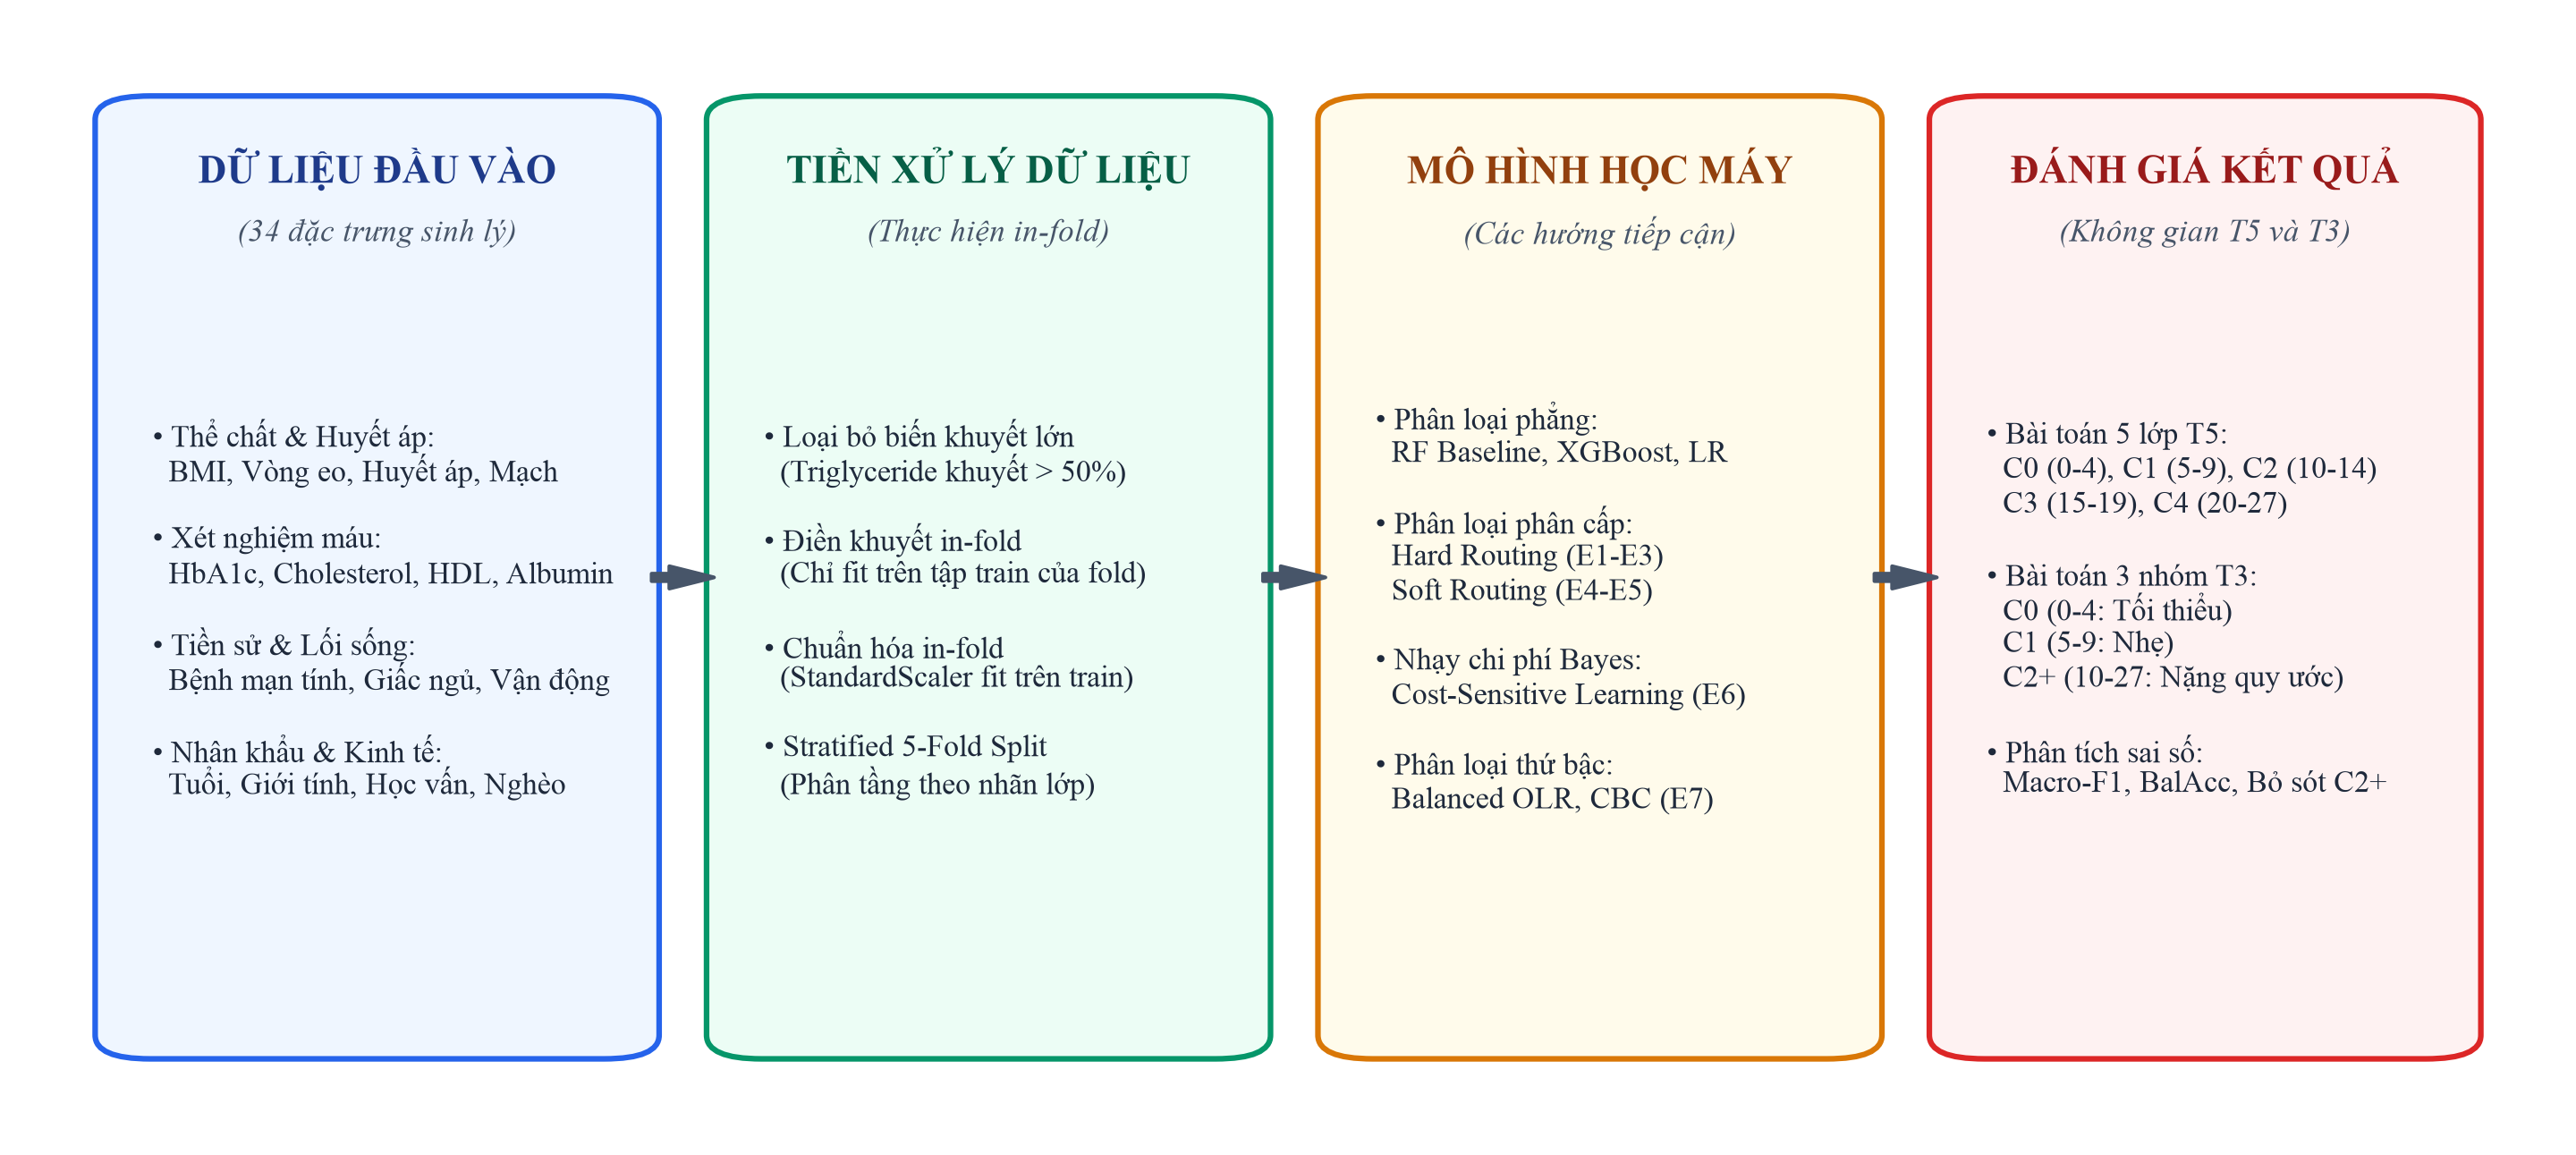
\includegraphics[width=\textwidth]{figures/fig1_problem_formulation.png}
\label{fig:problem-formulation}
\end{figure}
\FloatBarrier

\textbf{Nguyên tắc kiểm soát rò rỉ dữ liệu in-fold (In-Fold Preprocessing):} Để kết quả đánh giá phản ánh đúng khả năng khái quát hóa trên dữ liệu chưa thấy, ma trận đặc trưng đầu vào $\mathbf{X}$ không chứa bất kỳ câu hỏi nào trong 9 mục khảo sát DPQ. Tất cả các bước chuẩn hóa, điền khuyết (imputation) và mã hóa đặc trưng đều được học độc lập trên tập huấn luyện của từng fold kiểm định chéo và áp dụng nhất quán sang tập kiểm tra tương ứng.

\section{Mục tiêu và câu hỏi nghiên cứu}
\label{sec:muc-tieu-va-cau-hoi}

Mục tiêu tổng quát của đề tài là xây dựng một quy trình thực nghiệm học máy rõ ràng, có khả năng tái lập, nhằm khảo sát hiệu năng và giới hạn của việc dự đoán mức độ triệu chứng trầm cảm từ dữ liệu sinh lý NHANES.

Đề tài tập trung trả lời năm câu hỏi nghiên cứu (Research Questions -- RQ):
\begin{itemize}
    \item \textbf{RQ1 (Đóng góp của các nhóm đặc trưng):} Những nhóm đặc trưng nào (trong số nhân trắc, huyết áp, xét nghiệm máu, lối sống và nhân khẩu học) đóng góp nhiều nhất vào khả năng phân loại mức độ PHQ-9, và việc kết hợp các nhóm này có cải thiện hiệu năng so với từng nhóm riêng rẽ không?
    \item \textbf{RQ2 (Xu hướng suy giảm theo độ chi tiết nhãn):} Hiệu năng mô hình thay đổi ra sao khi tăng số lớp từ 2 lên 3, 4 và 5 mức độ? Ranh giới phân lớp nào gây ra mức sụt giảm lớn nhất?
    \item \textbf{RQ3 (Ảnh hưởng của việc tăng quy mô dữ liệu):} Việc mở rộng cỡ mẫu từ một chu kỳ đơn lẻ ($N = 5.054$) lên ba chu kỳ gộp ($N = 14.581$) với các đặc trưng hài hòa có giúp cải thiện hiệu năng ở các mức độ chi tiết hay không?
    \item \textbf{RQ4 (Hiệu quả của phân loại phân cấp hai bước):} Kiến trúc phân loại phân cấp (Hierarchical Classification) trên không gian 3 nhóm ($T_3$) thể hiện ra sao so với phân loại phẳng truyền thống (Flat Classification), và cơ chế định tuyến cứng (Hard Routing) dẫn đến sai số một chiều như thế nào?
    \item \textbf{RQ5 (Vai trò của Soft, Cost-Sensitive và Ordinal Classification):} Việc áp dụng định tuyến mềm (Soft Voting Fusion), lý thuyết quyết định nhạy chi phí Bayes và phân loại thứ bậc (Ordinal Classification) giúp điều chỉnh sự đánh đổi giữa Macro-F1, Balanced Accuracy và số ca nặng bị bỏ sót như thế nào?
\end{itemize}

\section{Phạm vi và giới hạn nghiên cứu}
\label{sec:pham-vi-nghien-cuu}

Các giới hạn nghiên cứu của đề tài bao gồm:
\begin{enumerate}
    \item \textbf{Nguồn dữ liệu:} Nghiên cứu sử dụng dữ liệu khảo sát cắt ngang dạng bảng của NHANES (Hoa Kỳ) các chu kỳ 2011--2012, 2013--2014 và 2015--2016, áp dụng cho người tham gia từ 20 tuổi trở lên có đủ 9 mục khảo sát PHQ-9.
    \item \textbf{Dạng đặc trưng:} Đề tài chỉ sử dụng các đặc trưng sinh lý, cận lâm sàng và nhân khẩu dạng bảng trích xuất từ hồ sơ khám sức khỏe định kỳ. Nghiên cứu \textbf{không sử dụng tín hiệu chuỗi thời gian thô} như điện tâm đồ (ECG) hay điện não đồ (EEG).
    \item \textbf{Mục đích sử dụng:} Đề tài tập trung vào bài toán sàng lọc mức độ triệu chứng tự báo cáo trong nghiên cứu dịch tễ học, \textbf{không phải công cụ chẩn đoán bệnh học lâm sàng}. Kết quả dự đoán không thay thế quy trình thăm khám và đánh giá của bác sĩ tâm thần.
    \item \textbf{Phương pháp học máy:} Nghiên cứu tập trung thử nghiệm và so sánh các kiến trúc mô hình học máy dạng bảng (phẳng, phân cấp, nhạy chi phí và thứ bậc) để tìm hiểu đặc điểm dữ liệu thực tế.
\end{enumerate}

\section{Phương pháp tiếp cận và hai hướng nghiên cứu thực nghiệm}
\label{sec:dong-gop-nghien-cuu}

Nghiên cứu được triển khai theo hai hướng thực nghiệm có mối liên hệ mật thiết với nhau, được minh họa trong Hình \ref{fig:research-progression}.

\begin{figure}[htbp]{Sơ đồ mối liên hệ giữa hai hướng nghiên cứu thực nghiệm trong DepSev-ML}
\centering
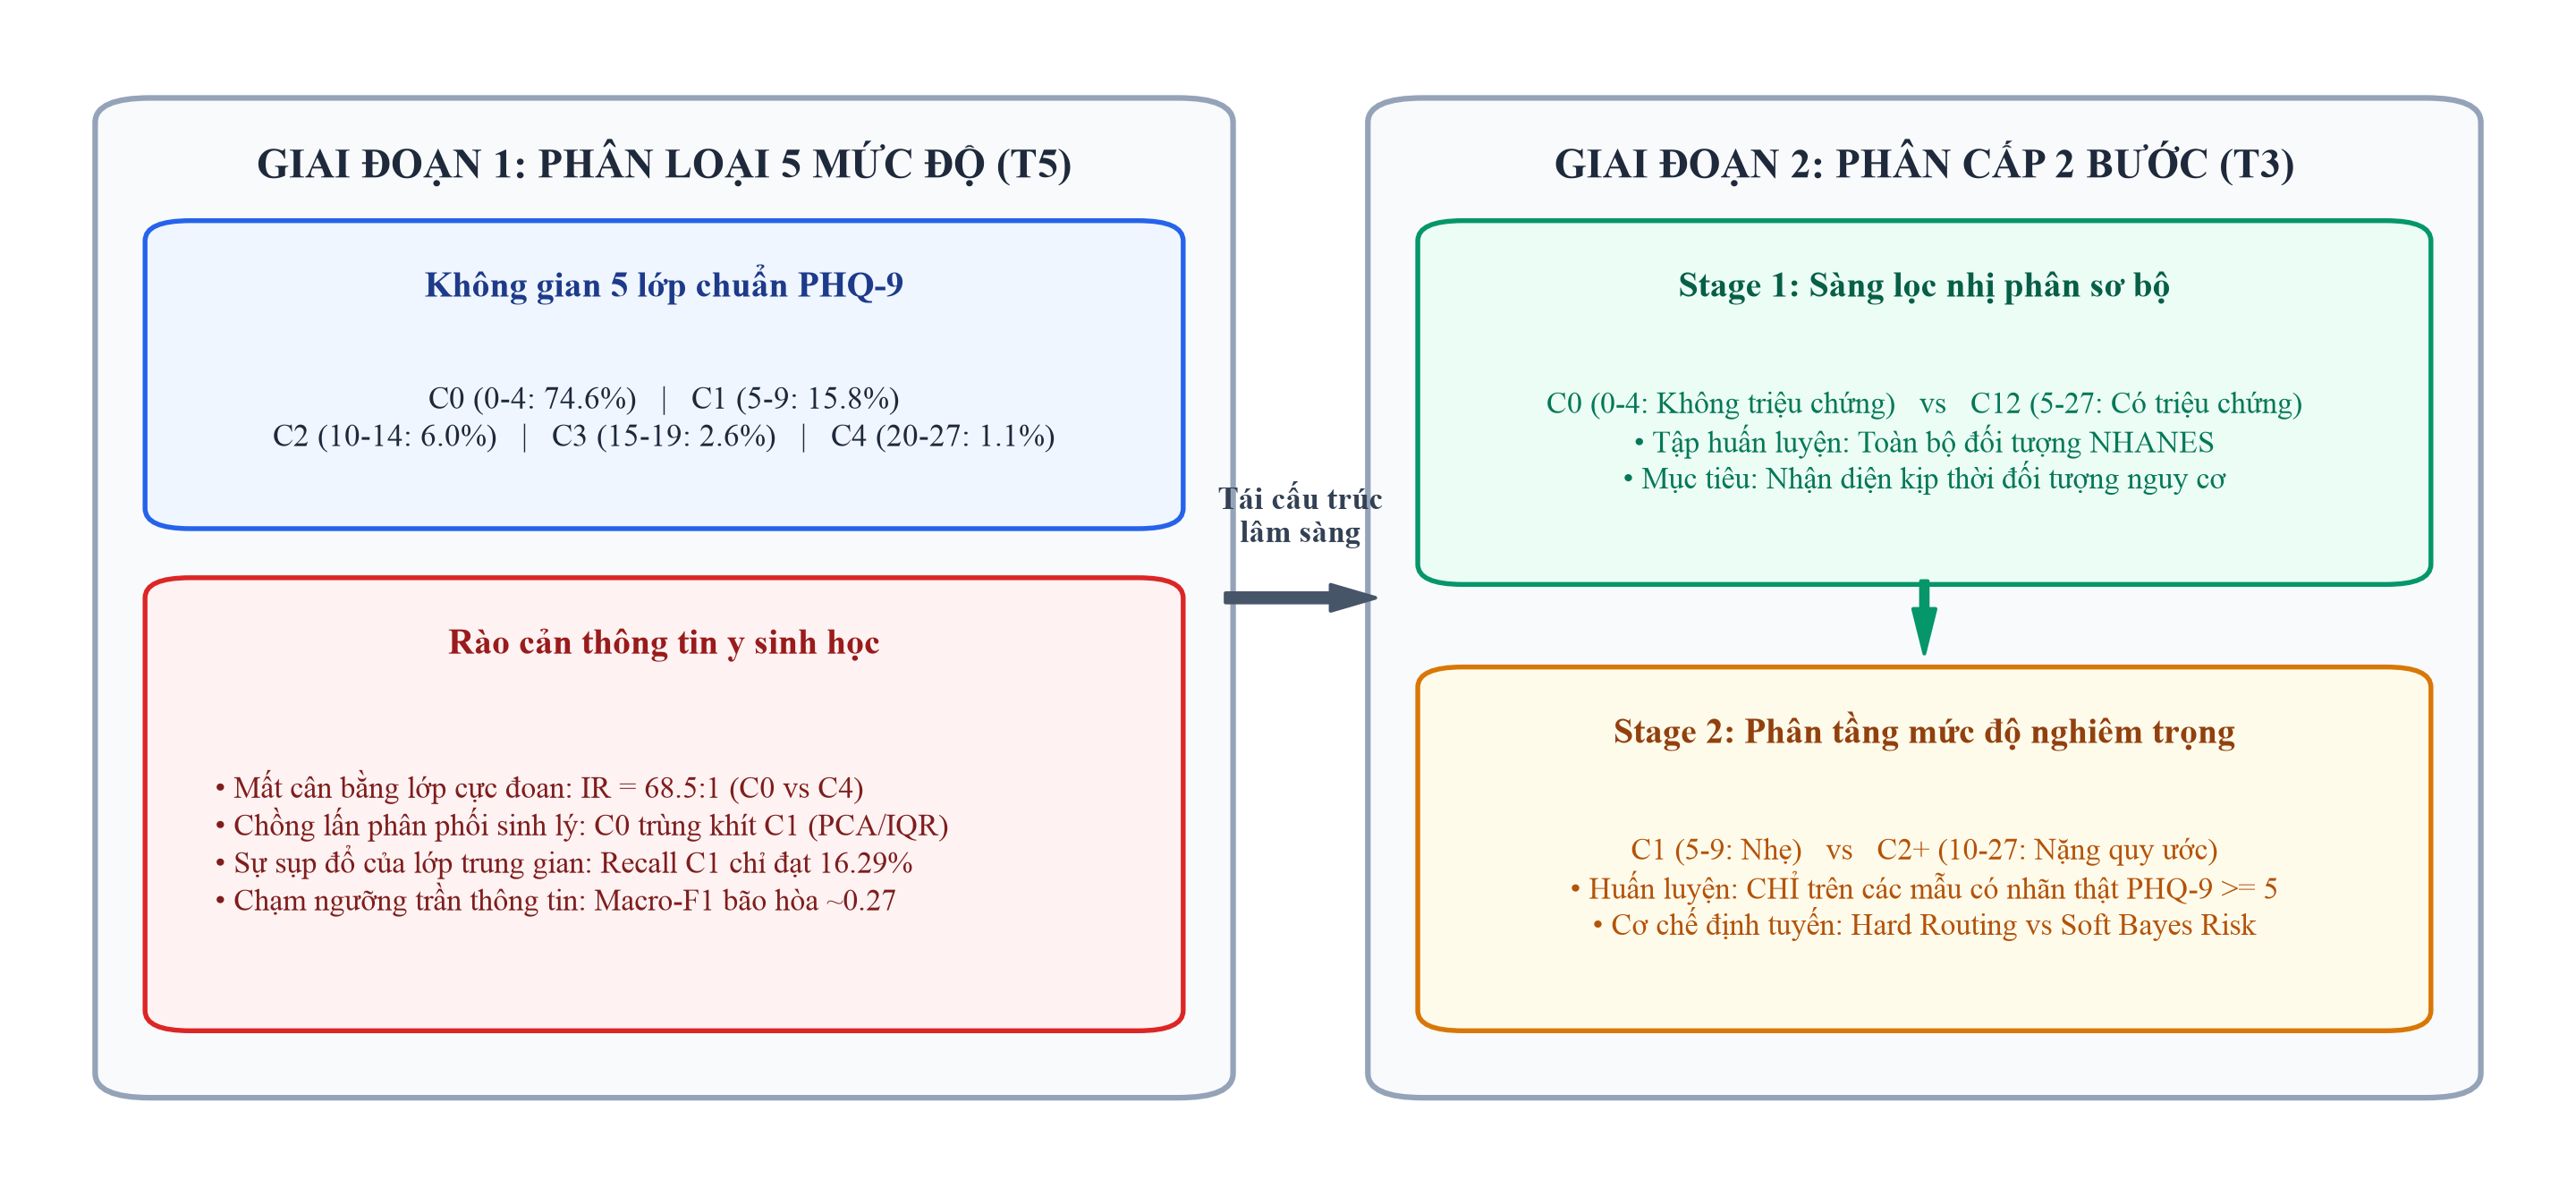
\includegraphics[width=\textwidth]{figures/fig_research_progression_t5_to_t3.png}
\label{fig:research-progression}
\end{figure}
\FloatBarrier

\begin{enumerate}
    \item \textbf{Hướng 1 -- Khảo sát bài toán phân loại đa mức trên không gian 5 mức độ tiêu chuẩn ($T_5$):} 
    Nghiên cứu khảo sát 4 thuật toán học máy phổ biến gồm Logistic Regression, Decision Tree, Random Forest và XGBoost để dự đoán năm mức độ triệu chứng theo thang đo PHQ-9 ($C_0$: $0$--$4$, $C_1$: $5$--$9$, $C_2$: $10$--$14$, $C_3$: $15$--$19$, $C_4$: $20$--$27$). Dựa trên quy trình kiểm định chéo lồng nhau (Nested CV), Random Forest được lựa chọn làm mô hình đối chuẩn (baseline) chính nhờ đạt được sự cân bằng giữa khả năng mô hình hóa phi tuyến và tính ổn định phương sai. Trên không gian $T_5$, nghiên cứu thực hiện đánh giá đóng góp đặc trưng (Feature Ablation $F_1 \to F_4$), khảo sát sự biến thiên hiệu năng theo độ chi tiết nhãn ($T_2 \to T_5$), thử nghiệm các mô hình kết hợp Ensemble và mở rộng cỡ mẫu đa chu kỳ ($N = 14.581$). Các phân tích định lượng (tương quan Spearman, liên hệ Cramer's V và trực quan hóa PCA 2D) giúp làm rõ mức độ chồng lấn phân phối sinh lý ngoại vi giữa các nhóm triệu chứng kế cận, đặc biệt giữa nhóm tối thiểu $C_0$ và nhóm nhẹ $C_1$.
    
    \item \textbf{Hướng 2 -- Khảo sát các hướng tiếp cận phân loại phân cấp và thứ bậc trên không gian 3 nhóm ($T_3$):} 
    Từ các quan sát thực nghiệm về đặc điểm ranh giới trên $T_5$, nghiên cứu mở rộng việc khảo sát sang bài toán 3 nhóm ($C_0$: Tối thiểu, $C_1$: Nhẹ, $C_2^+$: Nặng theo quy ước nghiên cứu, với điểm PHQ-9 $\ge 10$) nhằm so sánh có đối chứng các hướng tiếp cận mô hình hóa khác nhau ($E_0 \to E_7$):
    \begin{itemize}
        \item \textit{Phân loại phẳng đối chuẩn ($E_0$):} Dự đoán trực tiếp trên 3 lớp bằng thuật toán Random Forest.
        \item \textit{Phân loại phân cấp hai giai đoạn định tuyến cứng ($E_1 \to E_3$):} Stage 1 nhận diện người có triệu chứng ($C_0$ vs $C_{12} = C_1 \cup C_2^+$); Stage 2 phân biệt nhẹ ($C_1$) và nặng theo quy ước ($C_2^+$), được huấn luyện \textbf{chỉ trên các mẫu có nhãn thật $\text{PHQ-9} \ge 5$}. Hướng tiếp cận này giúp khảo sát ảnh hưởng của cơ chế định tuyến cứng đối với sai số một chiều.
        \item \textit{Phân loại phân cấp định tuyến mềm kết hợp chi phí Bayes ($E_4 \to E_6$):} Kết hợp phân phối xác suất liên tục qua công thức xác suất toàn phần và áp dụng ma trận chi phí bất đối xứng nhằm điều chỉnh sự đánh đổi giữa việc giảm số ca nặng bị bỏ sót và mức độ báo động nhầm.
        \item \textit{Phân loại thứ bậc ($E_7$):} Khai thác cấu trúc trật tự tự nhiên của các mức độ triệu chứng thông qua mô hình Ordinal Logistic Regression và Phân loại nhị phân tích lũy.
    \end{itemize}
    Cần nhấn mạnh rằng $T_3$ và $T_5$ là hai nhiệm vụ phân loại độc lập với không gian nhãn và mục tiêu ứng dụng khác nhau. Việc khảo sát cả hai bài toán giúp cung cấp cái nhìn toàn diện về đặc tính của dữ liệu sinh lý dạng bảng trong các bài toán dự đoán triệu chứng trầm cảm.
\end{enumerate}

Những đóng góp chính của đề tài bao gồm:
\begin{enumerate}
    \item \textbf{Đánh giá thực nghiệm có kiểm soát về đóng góp của các nhóm đặc trưng:} Xây dựng quy trình đánh giá 4 thuật toán trên các không gian đặc trưng lũy tiến ($F_1 \to F_4$), làm rõ vai trò bổ trợ của tiền sử bệnh lý mạn tính, hành vi lối sống và nhân khẩu học so với các chỉ số cận lâm sàng ngoại vi đơn thuần.
    \item \textbf{Khảo sát và lượng hóa sự thay đổi hiệu năng theo độ chi tiết nhãn:} Khảo sát sự biến thiên hiệu năng từ bài toán nhị phân $T_2$ sang các bài toán đa mức $T_3, T_4, T_5$, kết hợp phân tích tương quan và trực quan hóa PCA để tìm hiểu đặc tính phân bố tại các ranh giới lớp liền kề.
    \item \textbf{Phân tích đặc điểm cơ học và sự đánh đổi của các cấu trúc phân cấp:} Phân tích cơ chế lan truyền sai số trong cấu trúc phân cấp định tuyến cứng ($T_3$); đồng thời khảo sát mô hình phân cấp mềm kết hợp lý thuyết quyết định nhạy chi phí Bayes nhằm định lượng sự đánh đổi giữa giảm thiểu ca nặng bị bỏ sót và tỷ lệ báo động nhầm.
    \item \textbf{Đánh giá hướng tiếp cận thứ bậc và kiểm định ngoại suy theo thời gian:} Khảo sát các mô hình Ordinal Classification nhằm khai thác mối quan hệ thứ bậc tự nhiên của thang đo PHQ-9, đồng thời kiểm tra độ ổn định của mô hình qua giao thức kiểm định ngoại suy trên chu kỳ khảo sát độc lập.
\end{enumerate}

\section{Cấu trúc báo cáo}
\label{sec:bo-cuc-khoa-luan}

Báo cáo dự án nghiên cứu gồm 5 chương:
\begin{itemize}
    \item \textbf{Chương 1: Giới thiệu} -- Trình bày bối cảnh nghiên cứu, phát biểu bài toán, mục tiêu, 5 câu hỏi nghiên cứu, phạm vi và tiến trình thực hiện.
    \item \textbf{Chương 2: Cơ sở lý thuyết và các nghiên cứu liên quan} -- Giới thiệu thang đo PHQ-9, đặc tính mất cân bằng lớp và chồng lấn đặc trưng trong dữ liệu y tế dạng bảng, thuật toán Random Forest và các hướng mô hình hóa (phẳng, phân cấp, thứ bậc).
    \item \textbf{Chương 3: Dữ liệu và phương pháp nghiên cứu} -- Trình bày nguồn dữ liệu NHANES, quy trình tiền xử lý, hệ thống 4 nhóm đặc trưng, các cấu hình mô hình thực nghiệm ($E_0 \to E_7$) và quy trình kiểm định chéo.
    \item \textbf{Chương 4: Thực nghiệm và thảo luận} -- Trình bày chi tiết các kết quả Feature Ablation, tối ưu hóa siêu tham số, phân tích độ chi tiết nhãn, mở rộng đa chu kỳ, so sánh các mô hình $E_0 \to E_7$ và kiểm định theo thời gian.
    \item \textbf{Chương 5: Kết luận và hướng phát triển} -- Tóm tắt các kết quả đạt được, thảo luận các giới hạn của dữ liệu và đề xuất hướng nghiên cứu tiếp theo.
\end{itemize}

\chapter{Cơ sở lý thuyết và các nghiên cứu liên quan}
\label{ch:co-so-ly-thuyet}

Chương này trình bày cơ sở sinh lý học và phương pháp luận học máy cho bài toán dự đoán mức độ triệu chứng trầm cảm từ dữ liệu sinh lý dạng bảng, đồng thời tổng hợp các công trình nghiên cứu tiền nhiệm. Nội dung chương gồm: (1) Cấu trúc thang đo PHQ-9 và các cơ chế sinh học liên quan; (2) Hai đặc thù của dữ liệu y tế dạng bảng gồm mất cân bằng lớp và chồng lấn phân phối đặc trưng; (3) Khảo sát các thuật toán cơ sở và phân tích chi tiết thuật toán Random Forest; (4) Ba hướng tiếp cận mô hình hóa gồm phân loại phẳng, phân loại phân cấp kết hợp lý thuyết quyết định nhạy chi phí Bayes, và phân loại thứ bậc; (5) Tổng hợp các nghiên cứu liên quan.

\section{Thang đo PHQ-9 và cơ sở sinh lý học của triệu chứng trầm cảm}
\label{sec:thang-do-phq9-va-sinh-ly}

\subsection{Cấu trúc thang đo PHQ-9 và phân khoảng mức độ}
\label{subsec:cau-truc-phq9}

Thang đo Sức khỏe Bệnh nhân 9 mục (Patient Health Questionnaire-9 -- PHQ-9) là công cụ sàng lọc tâm thần tự báo cáo được chuẩn hóa, do Kroenke, Spitzer và Williams phát triển \cite{kroenke2001phq, spitzer1999validation}. PHQ-9 gồm 9 câu hỏi phản ánh tần suất xuất hiện các biểu hiện trong vòng hai tuần gần nhất, tương ứng với tiêu chuẩn DSM-IV: (1) Giảm hứng thú hoặc niềm vui trong các hoạt động; (2) Cảm giác buồn bã, chán nản hoặc tuyệt vọng; (3) Rối loạn giấc ngủ; (4) Mệt mỏi, thiếu năng lượng; (5) Thay đổi cảm giác thèm ăn; (6) Cảm giác tự ti hoặc mặc cảm tội lỗi; (7) Giảm khả năng tập trung; (8) Vận động chậm chạp hoặc bồn chồn; (9) Ý nghĩ về cái chết hoặc tự làm hại bản thân.

Mỗi câu hỏi được chấm điểm theo thang Likert 4 mức độ từ 0 đến 3 (0: Hoàn toàn không; 1: Vài ngày; 2: Hơn một nửa số ngày; 3: Gần như mỗi ngày). Tổng điểm số $s = \sum_{j=1}^9 \text{DPQ}_j \in [0, 27]$ được ánh xạ thành 5 khoảng mức độ triệu chứng được minh họa trong Hình \ref{fig:phq9-tiers}.

\begin{figure}[htbp]{Thang đo PHQ-9 (0--27 điểm), 5 khoảng mức độ triệu chứng và ánh xạ sang không gian 3 nhóm $T_3$}
\centering
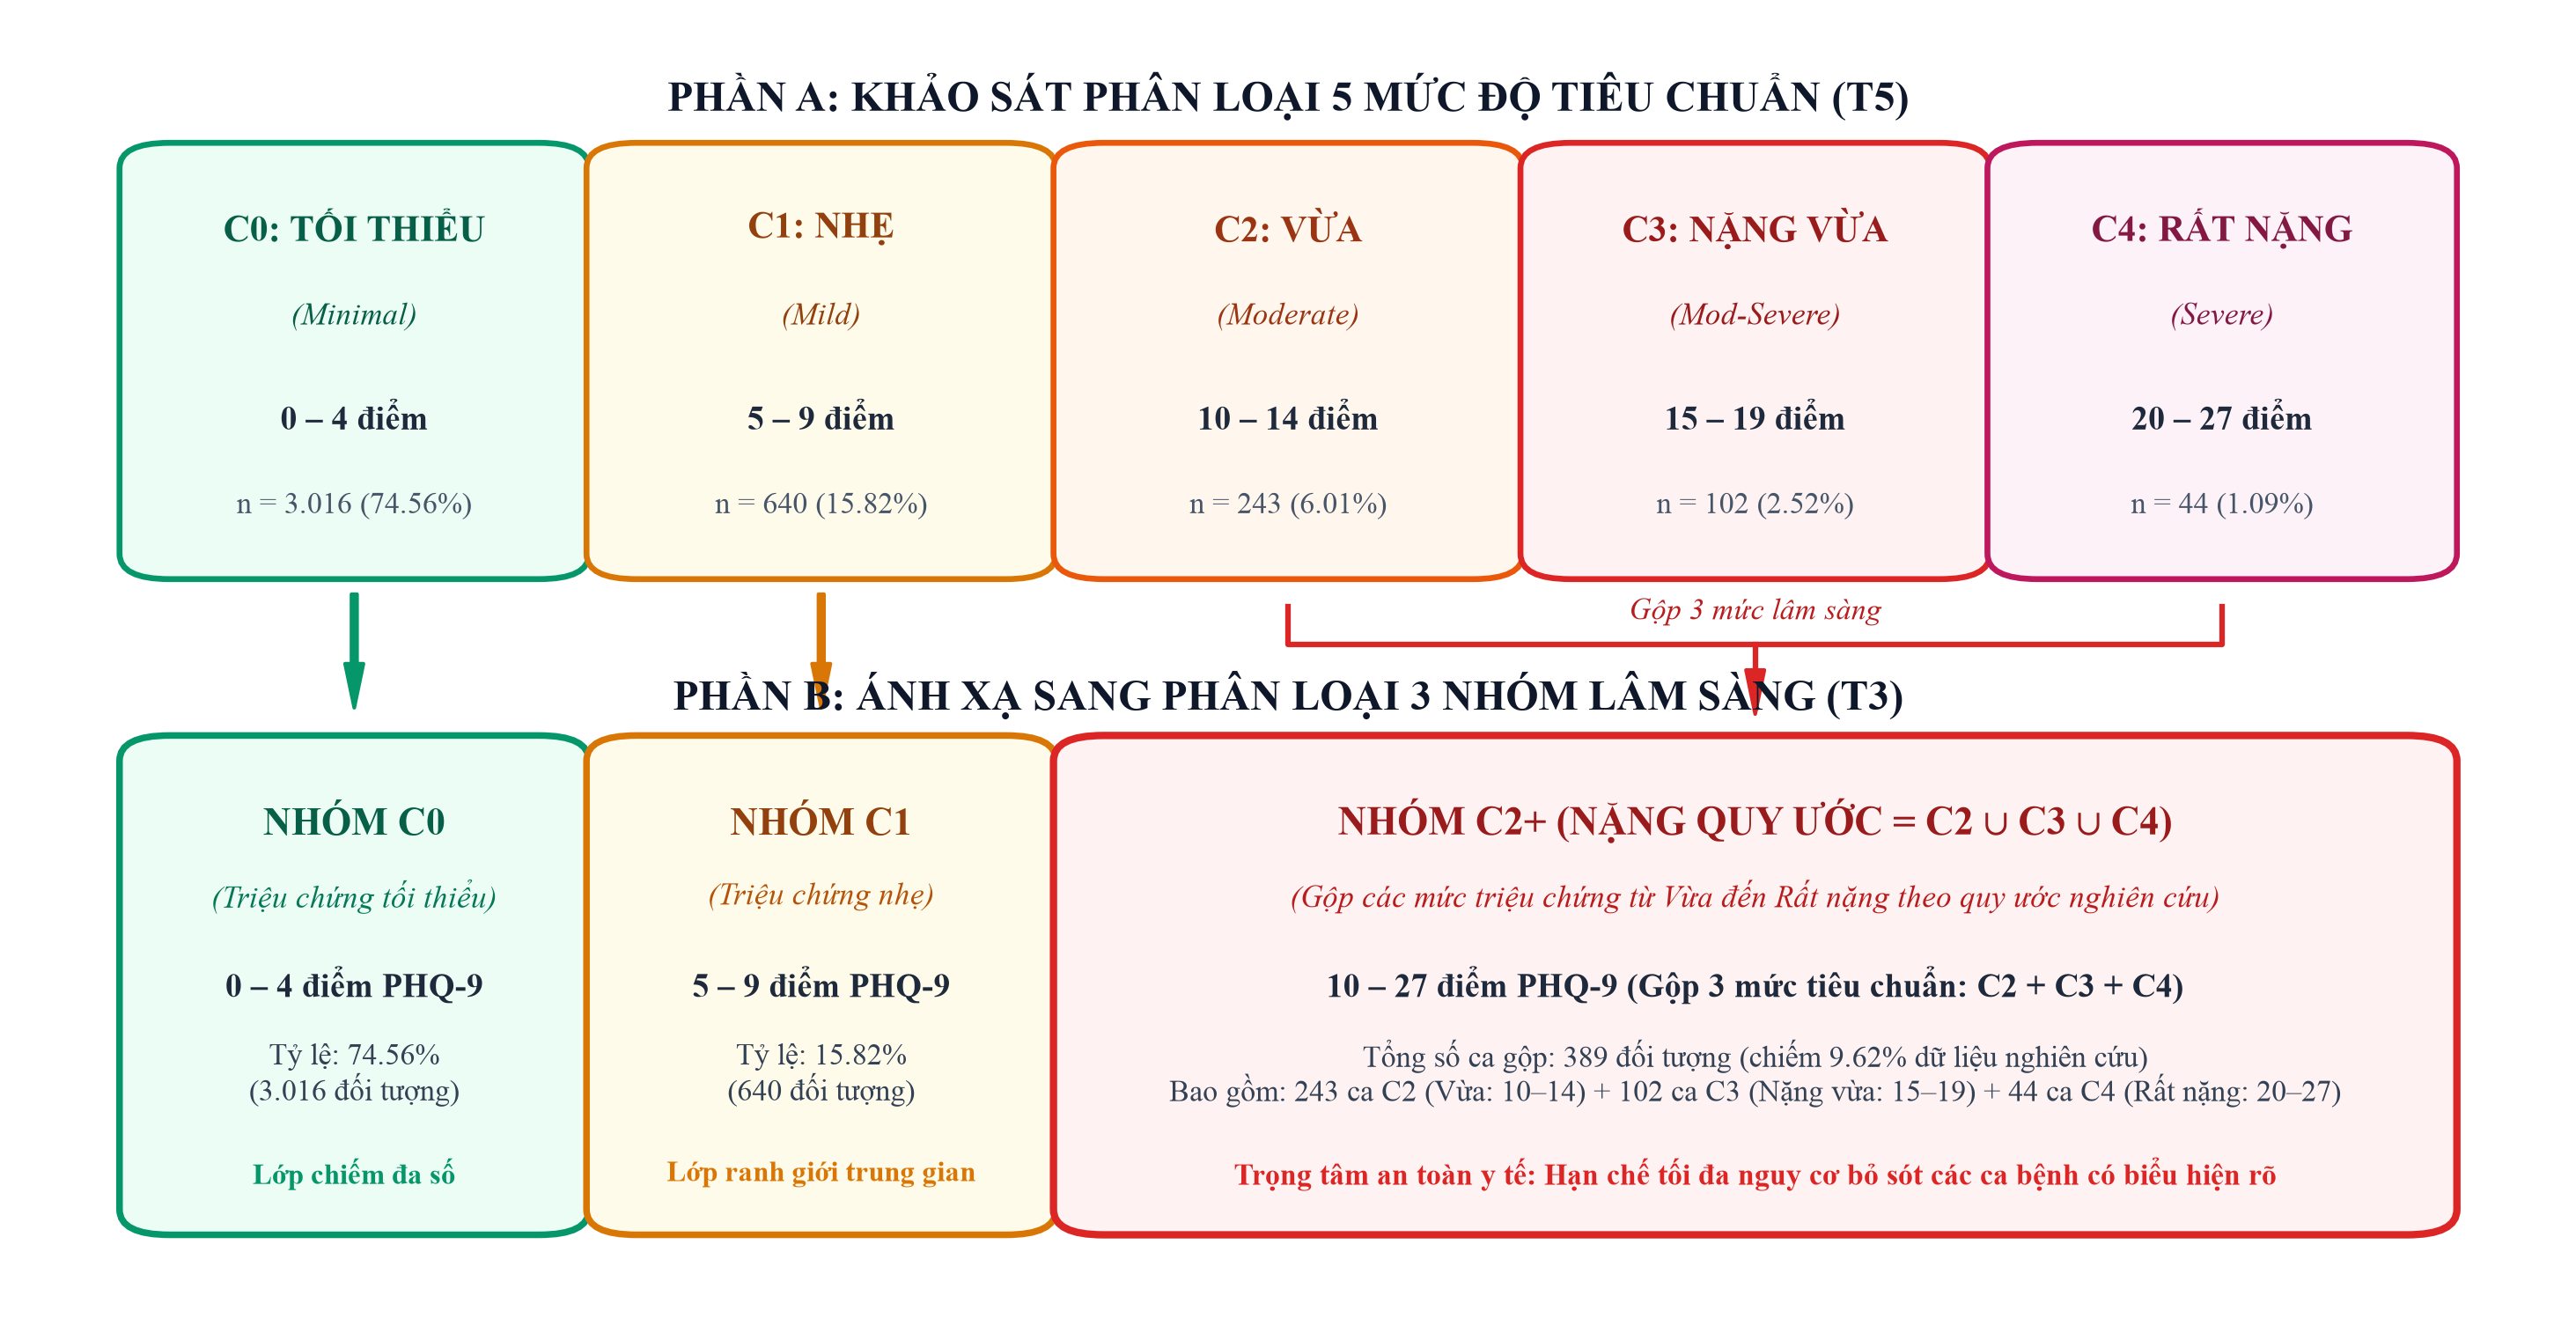
\includegraphics[width=\textwidth]{figures/fig2_phq9_tiers.png}
\label{fig:phq9-tiers}
\end{figure}
\FloatBarrier

Theo quy ước trong y văn:
\begin{itemize}
    \item $s \in [0, 4]$ ($C_0$ -- Tối thiểu): Mức triệu chứng tối thiểu, thường phản ánh trạng thái tâm lý ổn định theo thang đo tự điền.
    \item $s \in [5, 9]$ ($C_1$ -- Nhẹ): Mức độ triệu chứng nhẹ; trong sàng lọc cộng đồng thường được lưu ý theo dõi thêm.
    \item $s \in [10, 14]$ ($C_2$ -- Vừa): Mức độ triệu chứng trung bình; thường được xem là ngưỡng điểm gợi ý cần thăm khám chuyên sâu.
    \item $s \in [15, 19]$ ($C_3$ -- Nặng vừa): Mức độ triệu chứng nặng vừa theo thang đo PHQ-9.
    \item $s \in [20, 27]$ ($C_4$ -- Nặng): Mức độ triệu chứng nặng nhất theo thang đo PHQ-9.
\end{itemize}

Trong đề tài DepSev-ML, bên cạnh không gian 5 mức ban đầu ($T_5$), bài toán còn được khảo sát trên không gian 3 nhóm ($T_3$), trong đó nhóm $C_2^+$ đại diện cho toàn bộ các mẫu có điểm PHQ-9 $\ge 10$ ($C_2 \cup C_3 \cup C_4$), được gọi là nhóm Nặng theo quy ước nghiên cứu. Cần lưu ý rằng các khoảng điểm này đóng vai trò nhãn mục tiêu cho bài toán học máy, không đồng nghĩa với chẩn đoán xác định bệnh học lâm sàng.

\subsection{Cơ sở sinh lý học và các chỉ số liên quan}
\label{subsec:co-so-sinh-ly}

Dù triệu chứng trầm cảm thể hiện chủ yếu qua cảm xúc và hành vi, các nghiên cứu y sinh học ghi nhận mối liên hệ giữa trạng thái trầm cảm và một số rối loạn chuyển hóa, miễn dịch ngoại vi thông qua trục não-ruột và trục hạ đồi-tuyến yên-tuyến thượng thận (HPA) \cite{pratt2014depression}.

\begin{figure}[htbp]{Các cơ chế y sinh học liên kết chỉ số sinh lý ngoại vi với mức độ triệu chứng trầm cảm}
\centering
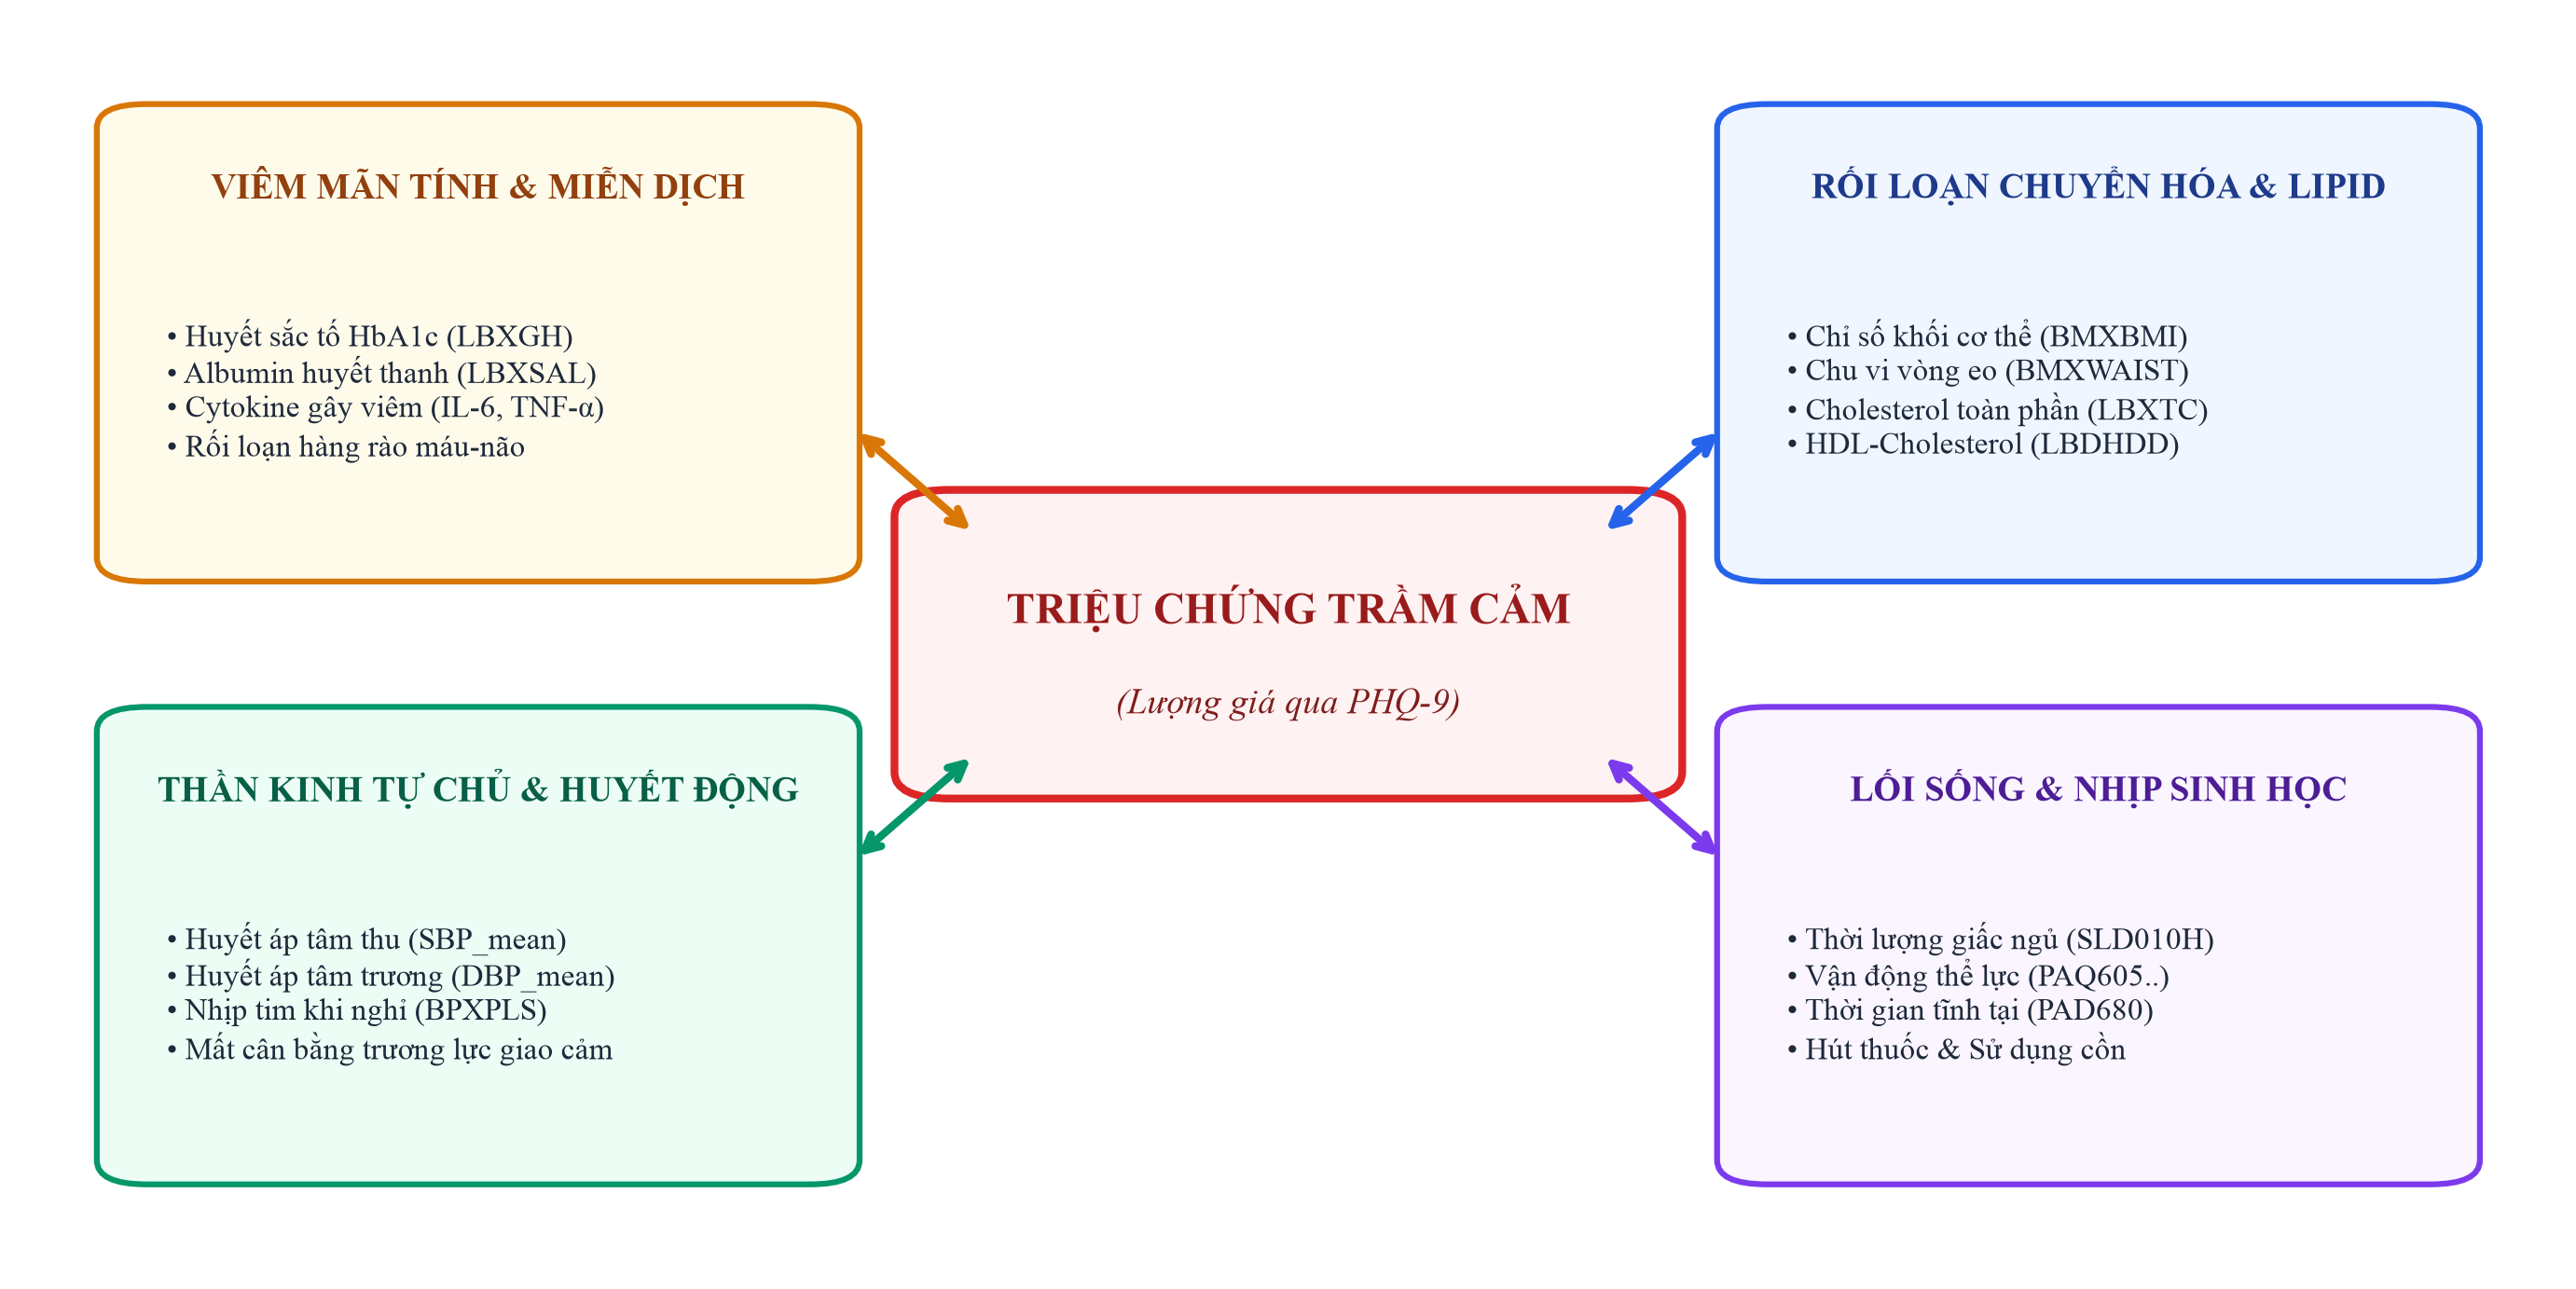
\includegraphics[width=\textwidth]{figures/fig2_gut_brain_metabolic_axis.png}
\label{fig:gut-brain-axis}
\end{figure}
\FloatBarrier

Như mô tả trong Hình \ref{fig:gut-brain-axis}, các nhóm biến số ngoại vi trong NHANES liên quan đến bốn cơ chế chính:
\begin{enumerate}
    \item \textbf{Phản ứng viêm và miễn dịch ngoại vi:} Trầm cảm có thể liên quan đến các cytokine gây viêm ngoại vi. Nồng độ Albumin huyết thanh (LBXSAL) phản ánh tình trạng dinh dưỡng và protein huyết tương; chỉ số đường huyết tích lũy Glycohemoglobin HbA1c (LBXGH) phản ánh mức độ chuyển hóa glucose.
    \item \textbf{Chuyển hóa và lipid máu:} Hoạt động chuyển hóa thể hiện qua các chỉ số nhân trắc học như chỉ số khối cơ thể (BMXBMI), chu vi vòng eo (BMXWAIST), kết hợp cùng nồng độ Cholesterol toàn phần (LBXTC) và HDL-Cholesterol (LBDHDD).
    \item \textbf{Hệ thần kinh tự chủ và huyết áp:} Sự thay đổi trương lực giao cảm có thể ảnh hưởng đến nhịp tim khi nghỉ (BPXPLS), huyết áp tâm thu (SBP\_mean) và huyết áp tâm trương (DBP\_mean).
    \item \textbf{Hành vi lối sống:} Thời gian ngủ (SLD010H), mức độ hoạt động thể lực, thời gian ngồi tĩnh tại (PAD680) cùng với hành vi hút thuốc, uống rượu bia có mối tương quan đáng kể với sự gia tăng điểm số PHQ-9.
\end{enumerate}

\section{Đặc thù và thách thức của dữ liệu y tế dạng bảng}
\label{sec:dac-thu-du-lieu-bang}

Dữ liệu y tế dạng bảng trích xuất từ các khảo sát cộng đồng như NHANES có những đặc thù hình học phức tạp, khác biệt căn bản so với dữ liệu hình ảnh hay văn bản.

\subsection{Mất cân bằng lớp (Severe Class Imbalance)}
\label{subsec:mat-can-bang-lop}

Trong các cuộc điều tra dịch tễ học dân số, phần lớn người tham gia thuộc nhóm triệu chứng tối thiểu, trong khi nhóm có triệu chứng nặng chỉ chiếm tỷ lệ nhỏ. Tỷ số mất cân bằng (Imbalance Ratio -- IR) được tính bởi:
\begin{equation}
    \text{IR} = \frac{\max_k N_k}{\min_k N_k}
\end{equation}
Trong tập phát triển Legacy của nghiên cứu ($N = 4.045$), lớp $C_0$ chiếm $3.016$ đối tượng (74.56\%), trong khi lớp nặng nhất $C_4$ chỉ có $44$ đối tượng (1.09\%), tạo nên tỷ số mất cân bằng $\text{IR} = 3016 / 44 \approx 68.5:1$ (Hình \ref{fig:imbalance-overlap}a).

Nếu mô hình học máy huấn luyện nhằm tối thiểu hóa sai số toàn cục thông thường, thuật toán sẽ bị thiên lệch mạnh về phía lớp $C_0$, dẫn tới hiện tượng đạt độ chính xác Accuracy cao nhưng bỏ sót các ca có triệu chứng thực tế. Để giảm thiểu ảnh hưởng này, kỹ thuật gán trọng số nghịch đảo tần số lớp (Class-weighted objective) được áp dụng:
\begin{equation}
    w_k = \frac{N}{K \cdot N_k}
\end{equation}
nhằm cân bằng lại mức độ đóng góp của từng lớp trong quá trình tối ưu hàm mục tiêu.

\begin{figure}[htbp]{(a) Mất cân bằng lớp trên tập dữ liệu và (b) Hiện tượng chồng lấn phân phối đặc trưng sinh lý}
\centering
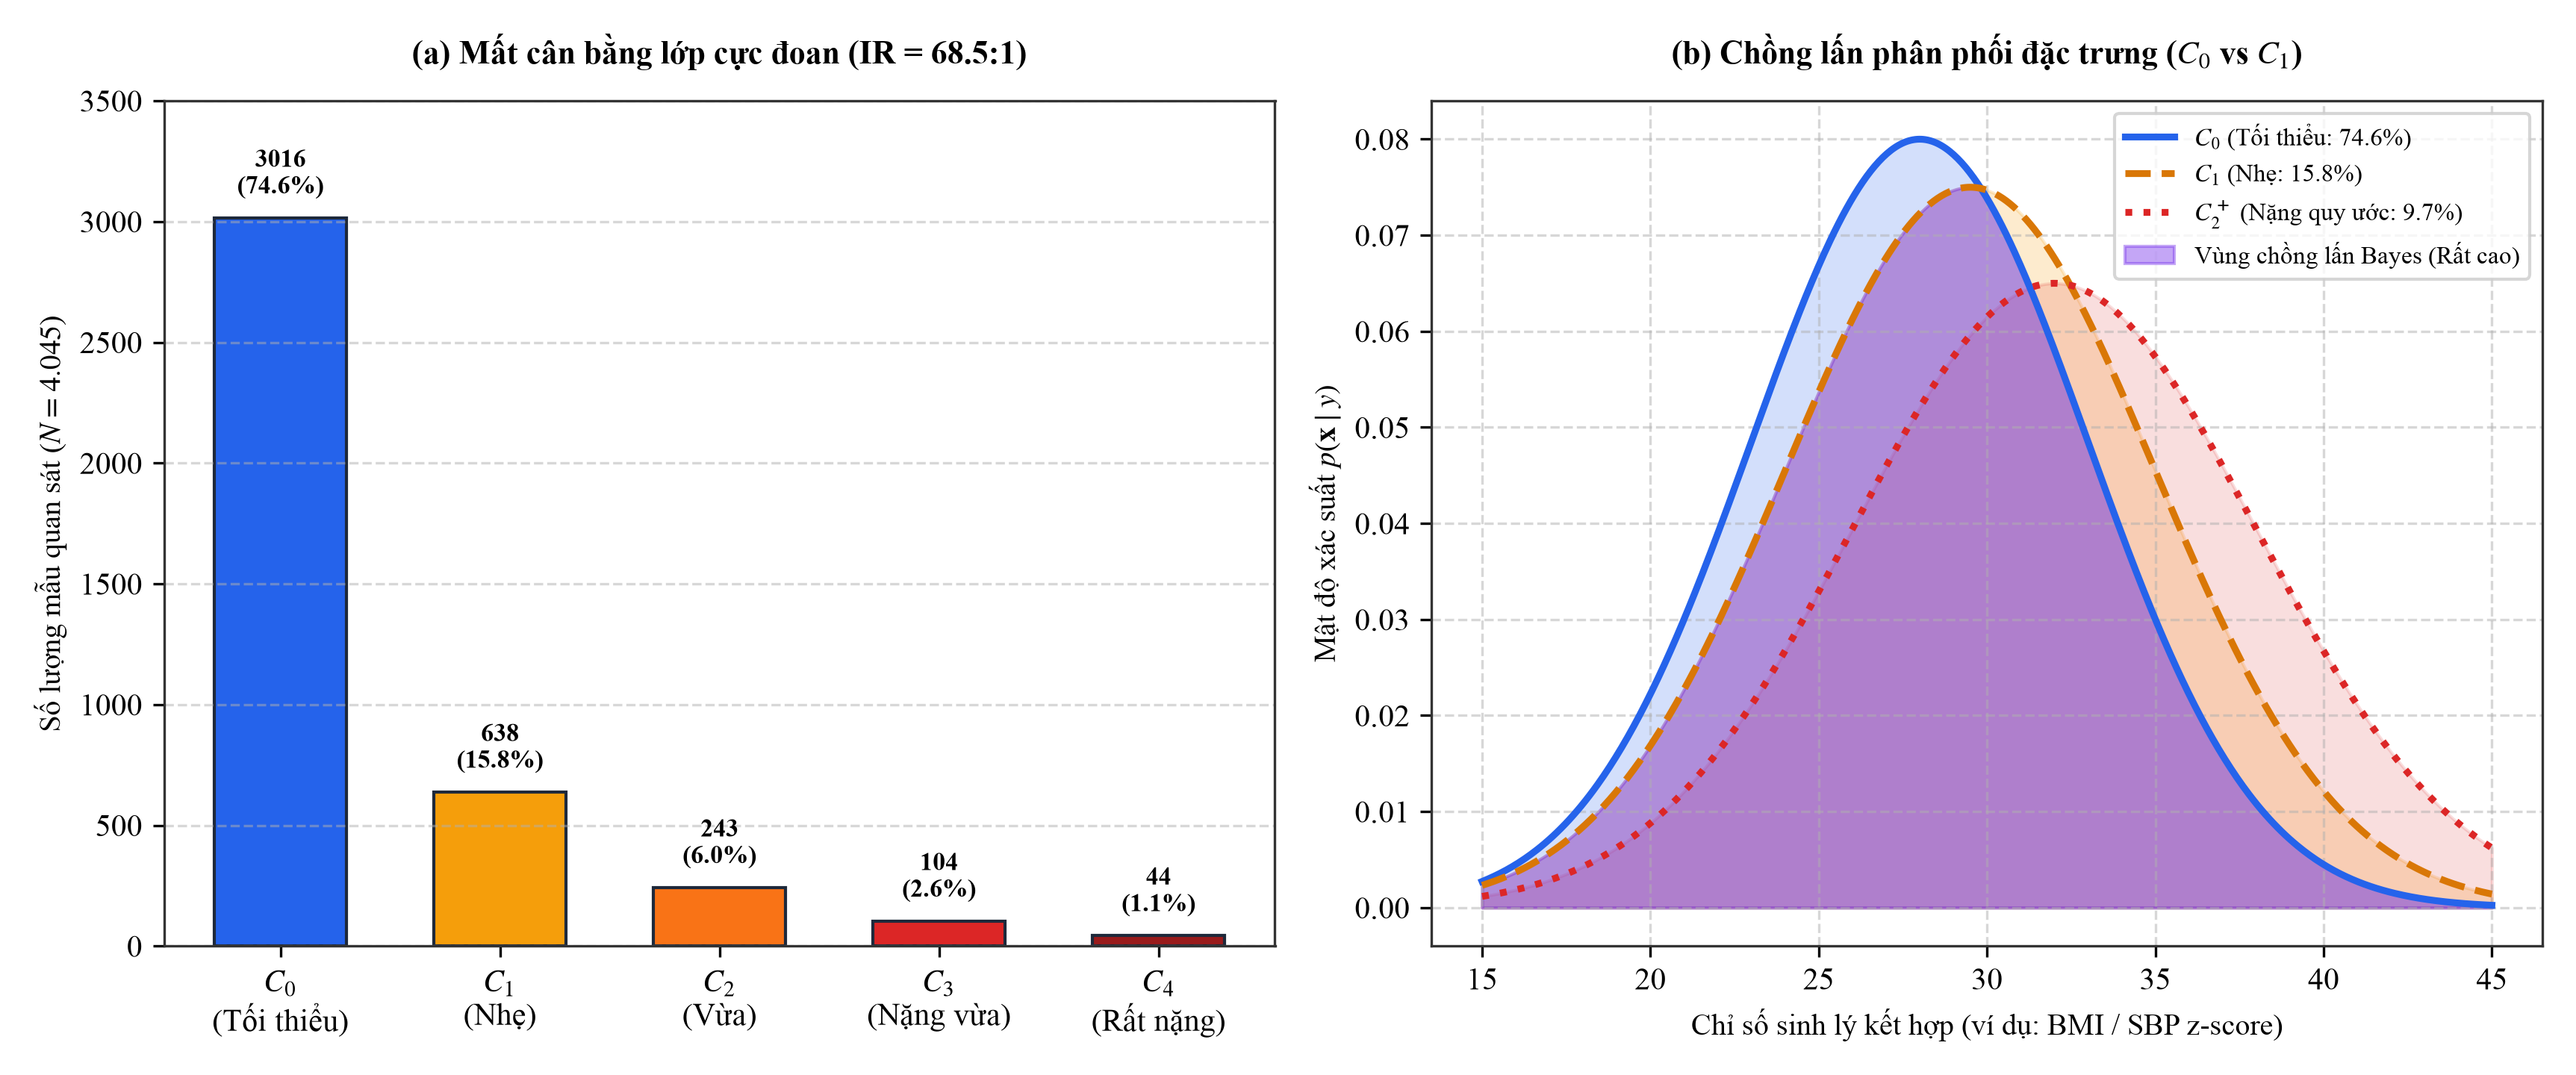
\includegraphics[width=\textwidth]{figures/fig2_imbalance_overlap.png}
\label{fig:imbalance-overlap}
\end{figure}
\FloatBarrier

\subsection{Chồng lấn phân phối đặc trưng (Feature Overlap)}
\label{subsec:chong-lan-dac-trung}

Khác với các xét nghiệm chẩn đoán đặc hiệu, các chỉ số sinh lý như huyết áp, cholesterol hay BMI không có một ngưỡng cắt sinh học duy nhất để phân tách rạch ròi người có triệu chứng tối thiểu và người có triệu chứng nhẹ. Phân phối xác suất điều kiện của đặc trưng $\mathbf{x}$ giữa hai trạng thái kế cận $p(\mathbf{x} \mid Y = 0)$ và $p(\mathbf{x} \mid Y = 1)$ có diện tích giao thoa rất lớn (Hình \ref{fig:imbalance-overlap}b).

Khi vùng giao thoa phân phối sinh lý giữa các lớp lớn, bộ phân loại không thể đạt được độ chính xác phân tách tuyệt đối nếu chỉ dựa vào các biến số sinh lý ngoại vi. Do đó, việc cải thiện hiệu năng đòi hỏi phải lựa chọn cấu trúc bài toán phù hợp và kiểm soát sự đánh đổi giữa các loại sai số.

\section{Khảo sát các thuật toán học máy cơ sở và Thuật toán Random Forest}
\label{sec:cac-thuat-toan-va-rf}

\subsection{Giới thiệu ngắn gọn các thuật toán học máy cơ sở}
\label{subsec:khao-sat-thuat-toan-co-so}

Để xây dựng và đánh giá các mô hình cơ sở (baselines), nghiên cứu đã thử nghiệm 4 thuật toán học máy phổ biến gồm Logistic Regression, Decision Tree, Random Forest và XGBoost:
\begin{itemize}
    \item \textbf{Logistic Regression (LR):} Mô hình tuyến tính kinh điển trong dịch tễ học, ước lượng xác suất hậu nghiệm thông qua hàm Sigmoid/Softmax, có ưu điểm tính toán nhanh và ổn định.
    \item \textbf{Decision Tree (DT):} Mô hình phi tuyến dựa trên các quy tắc phân nhánh nhị phân kiểu IF-THEN, không đòi hỏi chuẩn hóa biến số nhưng có phương sai lớn và nhạy cảm với biến động dữ liệu.
    \item \textbf{Random Forest (RF):} Phương pháp học kết hợp (Ensemble Learning) kết hợp nhiều cây quyết định độc lập qua kỹ thuật Bootstrap Sampling và ngẫu nhiên hóa đặc trưng.
    \item \textbf{XGBoost (XGB):} Thuật toán tăng cường độ dốc (Gradient Boosting) xây dựng chuỗi cây tuần tự để tối ưu hàm mất mát, có khả năng khớp các mối quan hệ phi tuyến mạnh mẽ.
\end{itemize}

Các thuật toán trên được huấn luyện và đánh giá trên cùng một quy trình kiểm định chéo lồng nhau (Nested Cross-Validation). Bảng so sánh kết quả thực nghiệm chi tiết giữa các thuật toán được trình bày tại Chương \ref{ch:thuc-nghiem} (Bảng \ref{tab:nested-cv-comparison}).

\textbf{Lý do lựa chọn Random Forest làm mô hình cơ sở chính:} Dựa trên kết quả Nested CV trên không gian 34 đặc trưng ($F_4$), Random Forest đạt Macro-F1 trung bình cao nhất ($0.2755 \pm 0.0270$) và Weighted-F1 đạt $0.6437 \pm 0.0087$. Dù Random Forest không dẫn đầu trên tất cả các chỉ số (chẳng hạn Logistic Regression có Balanced Accuracy nhỉnh hơn ở một số cấu hình), mô hình này mang lại sự cân bằng tốt giữa khả năng xử lý phi tuyến và tính ổn định phương sai trên dữ liệu y tế dạng bảng. Vì vậy, Random Forest được lựa chọn làm mô hình cơ sở chính (Backbone Model) cho các thí nghiệm tiếp theo trong nghiên cứu.

\subsection{Cấu trúc nền tảng: Nguyên lý hoạt động của Decision Tree}
\label{subsec:decision-tree-theory}

Để hiểu rõ Random Forest, trước hết cần nắm cách hoạt động của một Decision Tree đơn lẻ. Decision Tree phân tách đệ quy không gian đặc trưng đa chiều thành các vùng không gian con dạng siêu hình hộp chữ nhật (Hình \ref{fig:dt-concept}).

\begin{figure}[htbp]{Sơ đồ nguyên lý phân nhánh của Decision Tree trên không gian đặc trưng dạng bảng}
\centering
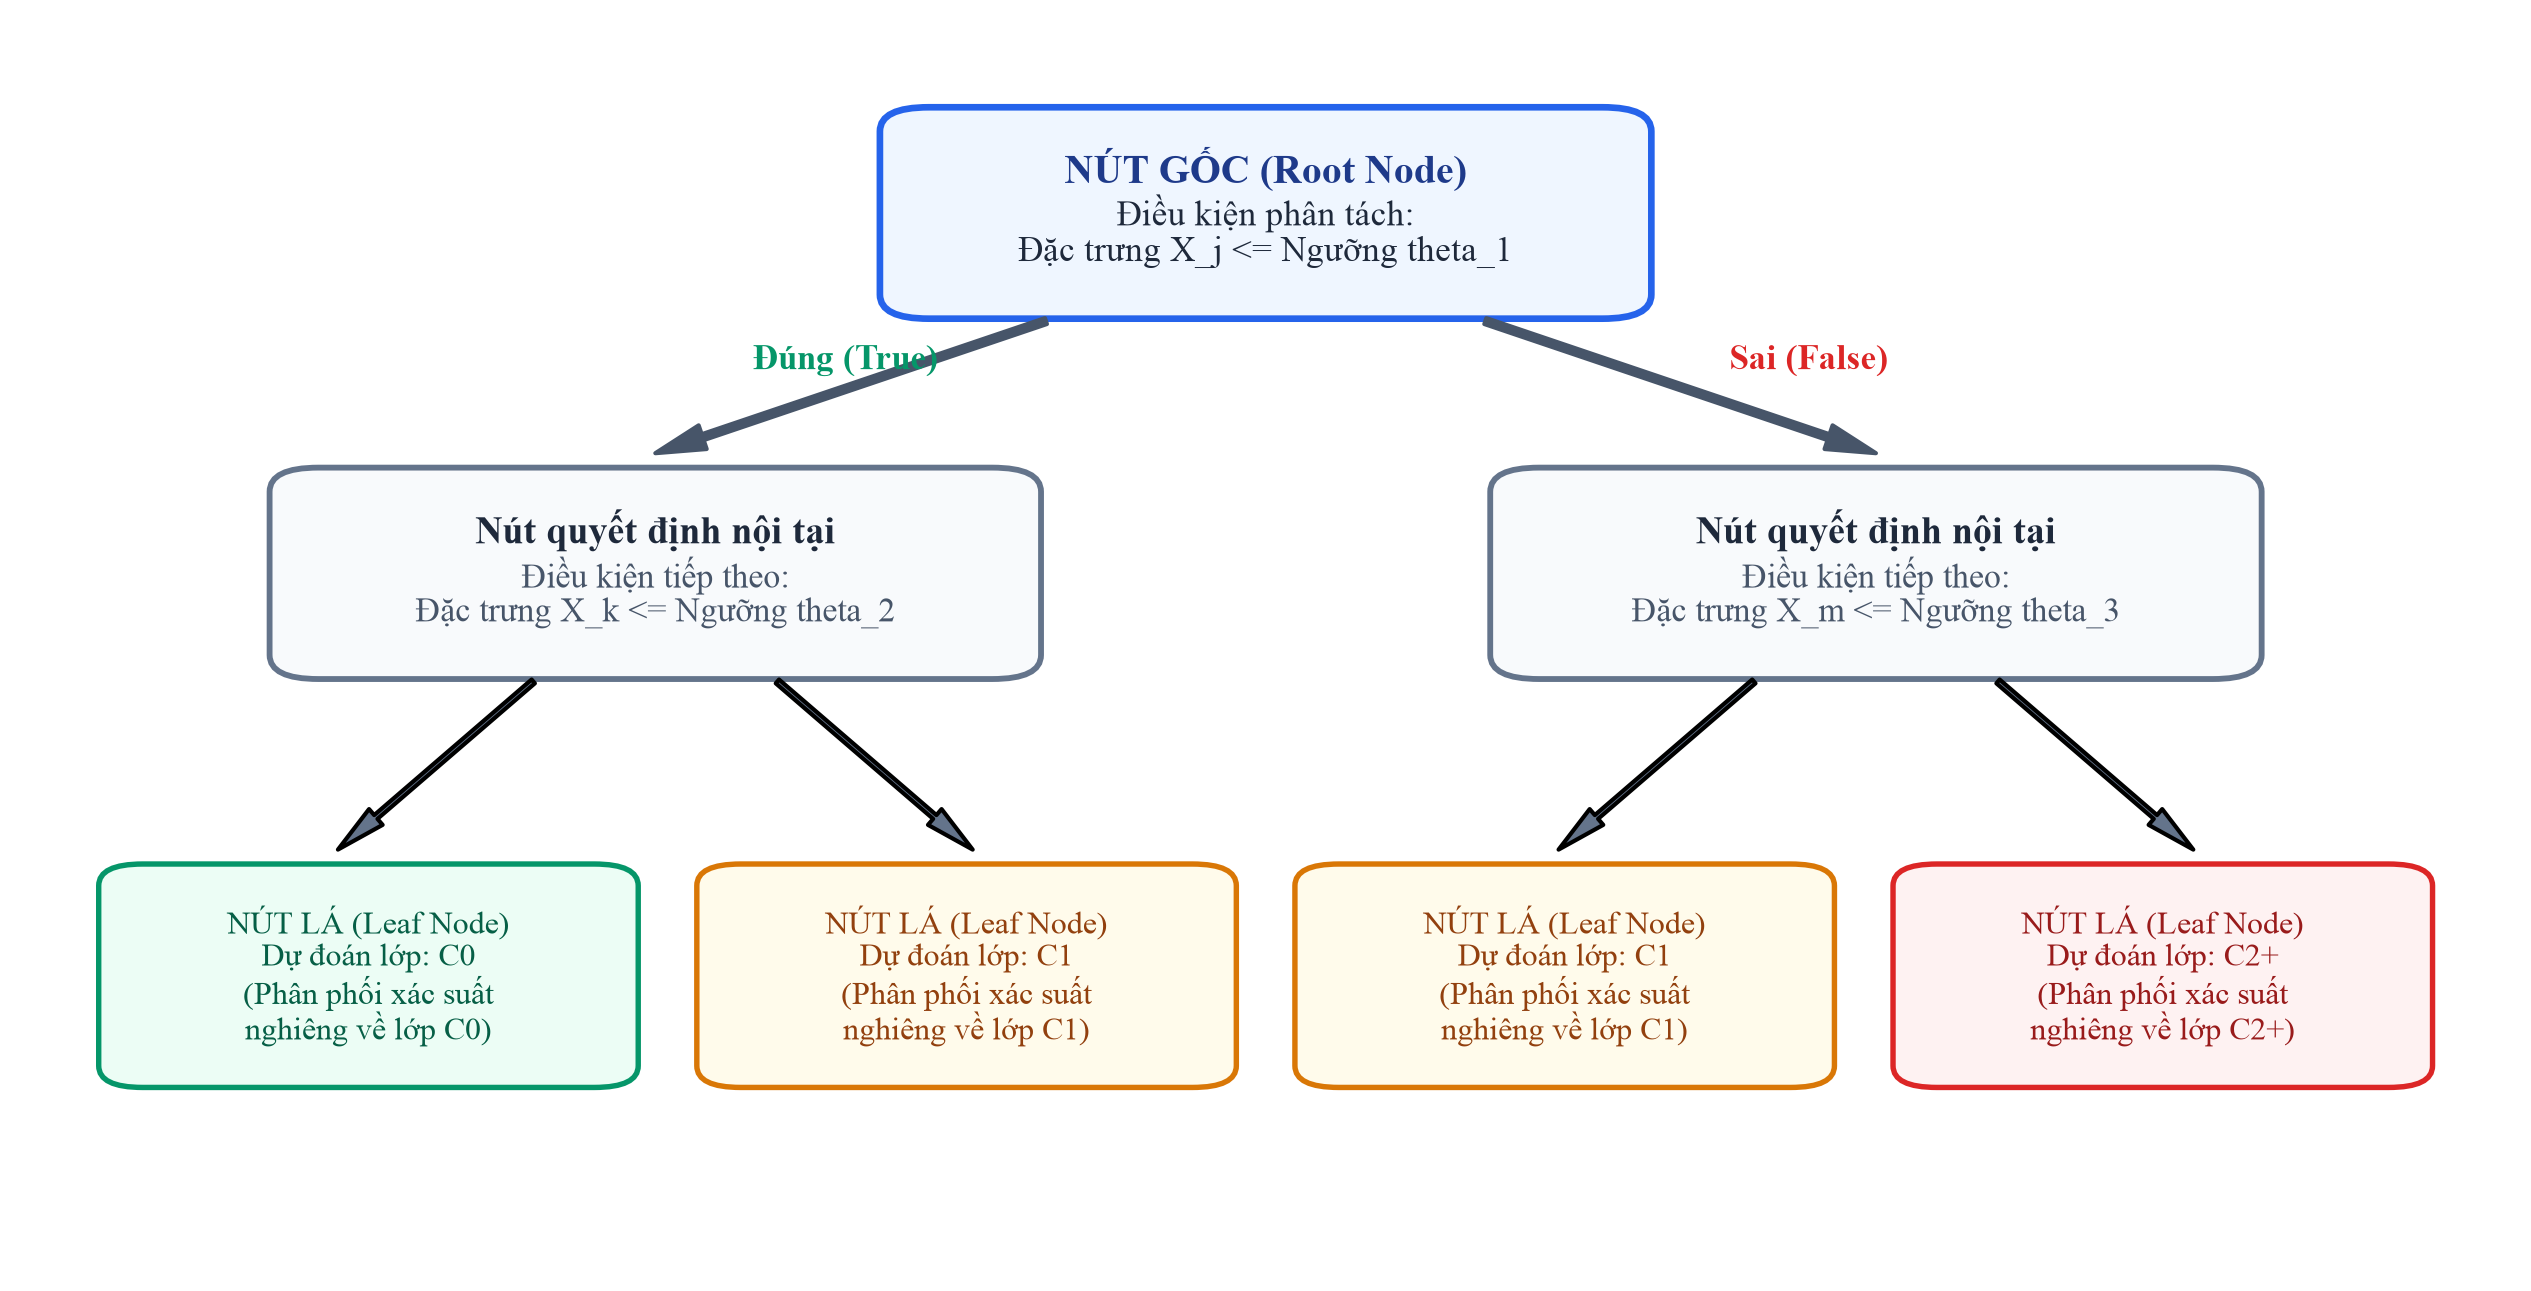
\includegraphics[width=0.88\textwidth]{figures/fig2_decision_tree_concept.png}
\label{fig:dt-concept}
\end{figure}
\FloatBarrier

Quá trình hoạt động của Decision Tree gồm:
\begin{enumerate}
    \item \textbf{Cấu trúc phân cấp:} Cây bắt đầu từ một nút gốc (Root Node) chứa toàn bộ tập dữ liệu huấn luyện, phân nhánh qua các nút quyết định (Decision Nodes) và kết thúc tại các nút lá (Leaf Nodes).
    \item \textbf{Quy tắc phân tách nhị phân:} Tại mỗi nút, thuật toán tìm kiếm đặc trưng $X_j$ và ngưỡng cắt $\theta$ tối ưu để chia dữ liệu thành hai nhánh con: $X_j \le \theta$ và $X_j > \theta$.
    \item \textbf{Tiêu chuẩn độ bất thuần Gini (Gini Impurity):} Cặp $(X_j, \theta)$ được chọn sao cho mức giảm độ bất thuần là lớn nhất. Chỉ số Gini tại một nút được định nghĩa:
    \begin{equation}
        G = 1 - \sum_{k=0}^{K-1} p_k^2
    \end{equation}
    trong đó $p_k$ là tỷ lệ mẫu thuộc lớp $k$ tại nút đó. Khi nút chỉ chứa mẫu của một lớp duy nhất, $G = 0$ (thuần khiết).
    \item \textbf{Dự đoán tại nút lá:} Khi cây đạt tiêu chuẩn dừng (độ sâu tối đa, số lượng mẫu tối thiểu tại lá), nút trở thành nút lá. Xác suất gán cho từng lớp tại lá là tỷ lệ mẫu thực tế của các lớp rơi vào vùng không gian con đó.
\end{enumerate}

\textbf{Hạn chế của Decision Tree đơn lẻ:} Một cây quyết định đơn lẻ có \textbf{phương sai cao (high variance)}. Do cây phân nhánh theo thuật toán tham lam từ trên xuống dưới, chỉ một biến động nhỏ trong dữ liệu huấn luyện (như một vài mẫu nhiễu) cũng có thể làm thay đổi quyết định phân tách ở nút gốc, kéo theo sự thay đổi toàn bộ cấu trúc các tầng bên dưới. Hiện tượng này khiến cây đơn lẻ dễ bị quá khớp (overfitting) trên dữ liệu y tế dạng bảng.

\subsection{Nguyên lý Random Forest và Cơ chế kết hợp nhiều cây}
\label{subsec:random-forest-deepdive}

Random Forest do Leo Breiman đề xuất năm 2001 \cite{breiman2001random} là phương pháp học kết hợp giúp giảm thiểu phương sai cao của cây đơn lẻ bằng cách xây dựng một tập hợp gồm $B$ cây quyết định độc lập (Hình \ref{fig:rf-concept}).

\begin{figure}[htbp]{Kiến trúc Random Forest: Bootstrap Sampling, ngẫu nhiên hóa đặc trưng và tổng hợp Soft Voting}
\centering
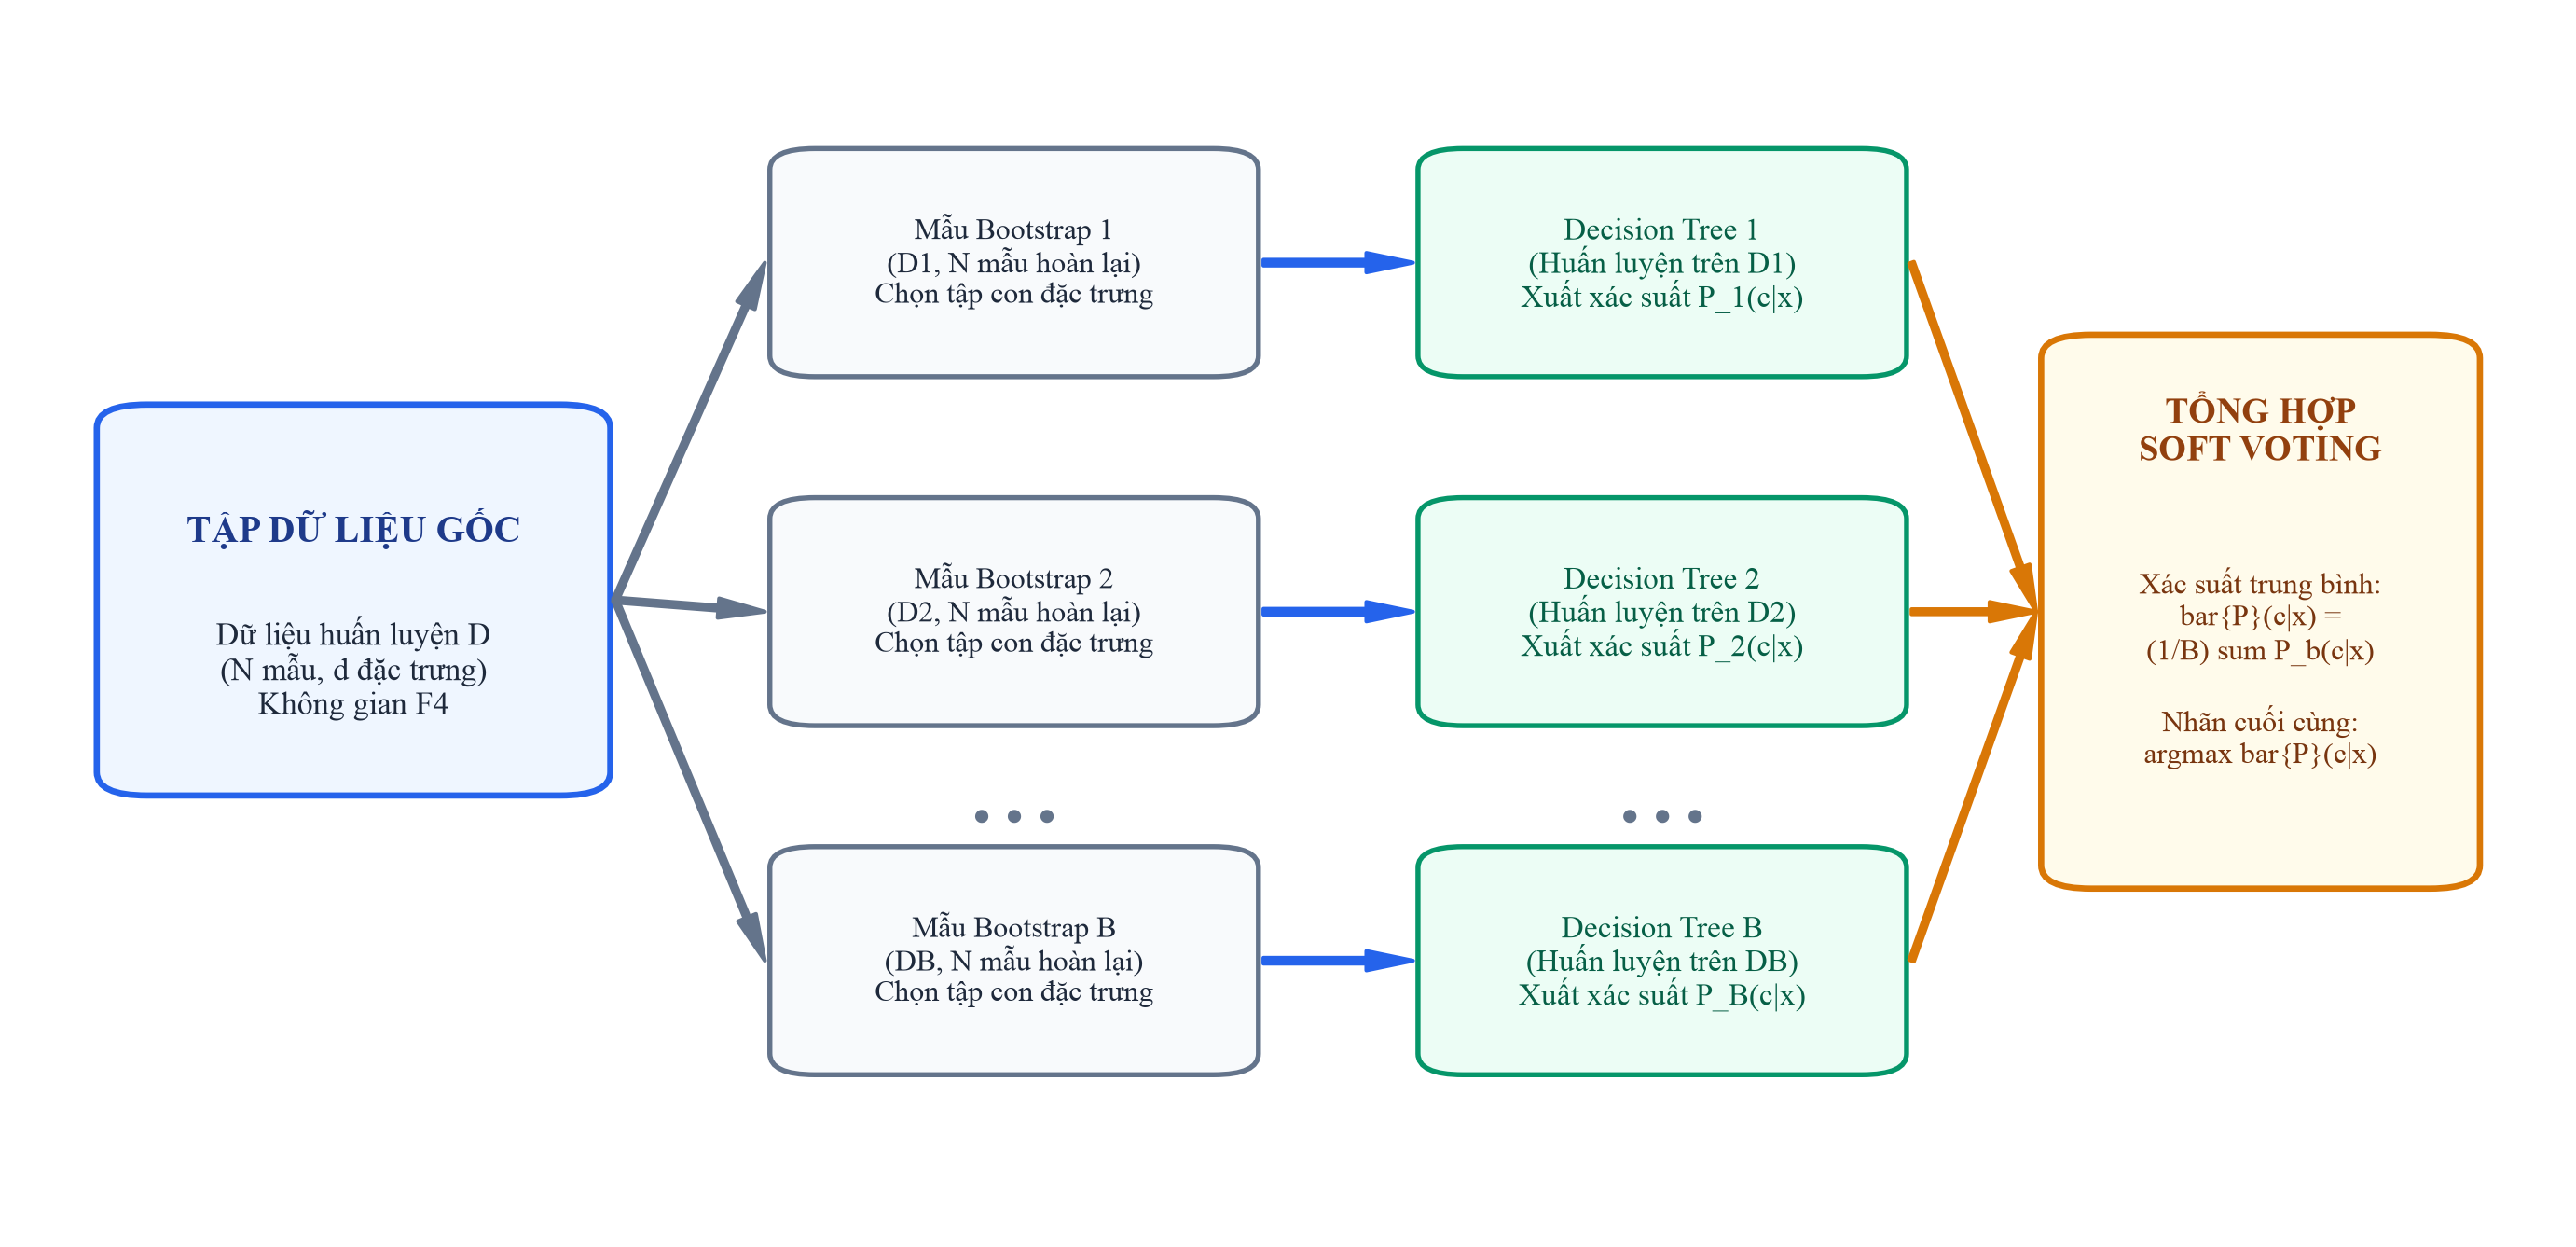
\includegraphics[width=\textwidth]{figures/fig2_random_forest_architecture.png}
\label{fig:rf-concept}
\end{figure}
\FloatBarrier

Random Forest vận hành dựa trên ba cơ chế chính:
\begin{enumerate}
    \item \textbf{Kỹ thuật Bootstrap Sampling:}
    Từ tập dữ liệu huấn luyện gốc gồm $N$ mẫu, thuật toán rút ngẫu nhiên có hoàn lại (sampling with replacement) đúng $N$ lần để tạo ra $B$ tập dữ liệu con độc lập $\mathcal{D}_1, \dots, \mathcal{D}_B$. Mỗi tập con chứa trung bình khoảng 63.2\% số mẫu độc nhất từ tập gốc, phần còn lại (khoảng 36.8\%) không xuất hiện trong tập huấn luyện của cây đó và được gọi là tập ngoài túi (Out-Of-Bag -- OOB).
    \item \textbf{Ngẫu nhiên hóa không gian đặc trưng (Feature Subspace Sampling):}
    Tại mỗi bước phân nhánh của từng cây con, Random Forest chỉ cho phép thuật toán chọn ngẫu nhiên một tập con gồm $m < d$ đặc trưng (trong nghiên cứu này đặt $m = 0.5 \times d$). Thuật toán chỉ tìm kiếm điểm cắt tối ưu trên tập con $m$ đặc trưng này. Nhờ đó, các cây con giảm bớt độ tương quan với nhau và khai thác thông tin từ nhiều góc nhìn khác nhau.
    \item \textbf{Cơ chế giảm phương sai bằng trung bình nhiều cây:}
    Việc lấy trung bình dự đoán từ nhiều cây quyết định được huấn luyện trên các tập mẫu và không gian đặc trưng ngẫu nhiên giúp làm giảm đáng kể phương sai ngẫu nhiên của từng cây đơn lẻ mà không làm tăng độ lệch (bias). Kết quả là mô hình tổng hợp đạt được tính ổn định và khả năng khái quát hóa tốt hơn nhiều so với một cây đơn lẻ.
\end{enumerate}

\subsection{Quy trình suy luận của một mẫu dữ liệu qua Random Forest}
\label{subsec:rf-inference-pipeline}

Khi một mẫu dữ liệu mới với vectơ đặc trưng $\mathbf{x} \in \mathbb{R}^d$ được đưa vào Random Forest, quy trình suy luận diễn ra qua các bước:
\begin{enumerate}
    \item Mẫu $\mathbf{x}$ được đưa đồng thời qua $B = 150$ cây quyết định trong rừng.
    \item Tại mỗi cây $b \in \{1, \dots, B\}$, mẫu di chuyển theo các ranh giới rẽ nhánh từ nút gốc xuống nút lá. Tỷ lệ các lớp mẫu tại nút lá tạo thành vectơ phân phối xác suất dự đoán của cây đó:
    \begin{equation}
        \mathbf{p}_b(\mathbf{x}) = \left[ P_b(Y = 0 \mid \mathbf{x}), \, P_b(Y = 1 \mid \mathbf{x}), \, \dots, \, P_b(Y = K-1 \mid \mathbf{x}) \right]^T
    \end{equation}
    \item Toàn bộ mô hình tổng hợp các dự đoán qua cơ chế \textbf{Soft Voting} (lấy trung bình cộng xác suất của tất cả các cây):
    \begin{equation}
        \bar{P}(Y = k \mid \mathbf{x}) = \frac{1}{B} \sum_{b=1}^B P_b(Y = k \mid \mathbf{x})
    \end{equation}
    Khác với Hard Voting (chỉ đếm số phiếu của lớp chiếm đa số), Soft Voting giữ lại độ tự tin định lượng của từng cây con, tạo ra phân phối xác suất trơn mượt phục vụ cho các bước phân cấp và tối ưu rủi ro chi phí tiếp theo.
    \item Trong mô hình phân loại phẳng, nhãn dự đoán cuối cùng là lớp có xác suất trung bình lớn nhất: $\hat{y} = \arg\max_k \bar{P}(Y = k \mid \mathbf{x})$.
\end{enumerate}

\subsection{Vai trò của các siêu tham số Random Forest trong dự án}
\label{subsec:rf-hyperparameters-role}

Trong dự án DepSev-ML, cấu hình Random Forest được cố định dựa trên kết quả tối ưu từ Nested CV:
\begin{itemize}
    \item \textbf{n\_estimators} = 150: Số lượng cây trong rừng. Giá trị $B = 150$ đủ để phân phối xác suất ổn định mà không gây tốn kém thời gian tính toán.
    \item \textbf{max\_depth} = 8: Độ sâu tối đa của từng cây. Giới hạn độ sâu ở mức 8 giúp cây không phân nhánh quá chi tiết để khớp các mẫu nhiễu, hạn chế tình trạng quá khớp.
    \item \textbf{max\_features} = 0.5: Tỷ lệ đặc trưng được chọn tại mỗi nút phân nhánh. Với không gian 34 biến ($F_4$), mỗi nút chỉ xem xét ngẫu nhiên 17 biến, giúp giảm độ tương quan giữa các cây khi có nhiều biến số cùng phản ánh một trục bệnh lý (như BMI và vòng eo).
    \item \textbf{min\_samples\_split} = 10 và \textbf{min\_samples\_leaf} = 8: Số mẫu tối thiểu để phân nhánh và tại nút lá, bảo đảm phân phối xác suất tại nút lá có đủ số lượng mẫu quan sát.
    \item \textbf{class\_weight} = \textnormal{'balanced\_subsample'}: Cơ chế điều chỉnh trọng số nghịch đảo tần số lớp trên từng mẫu bootstrap riêng biệt:
    \begin{equation}
        w_k^{(b)} = \frac{N^{(b)}}{K \cdot N_k^{(b)}}
    \end{equation}
    Kỹ thuật này giúp các cây quyết định chú ý hơn đến các mẫu thuộc lớp thiểu số trong từng lượt lấy mẫu.
\end{itemize}

\section{Các hướng tiếp cận mô hình hóa}
\label{sec:truong-phai-mo-hinh-hoa}

Trong bài toán dự đoán mức độ triệu chứng trầm cảm từ dữ liệu sinh lý, việc cấu trúc không gian bài toán và lựa chọn phương pháp học máy có ảnh hưởng lớn đến đặc tính phân loại và sự đánh đổi giữa các loại sai số. Nhằm khảo sát có hệ thống các khả năng mô hình hóa, nghiên cứu so sánh ba hướng tiếp cận chính được minh họa trong Hình \ref{fig:modeling-paradigms}:
\begin{enumerate}
    \item \textbf{Phương pháp phân loại phẳng (Flat Classification):} Xem các mức độ là các lớp danh nghĩa độc lập, đóng vai trò là mốc đối chuẩn truyền thống.
    \item \textbf{Phương pháp phân loại phân cấp (Hierarchical Classification):} Chia nhỏ bài toán thành quy trình hai giai đoạn kết hợp cơ chế định tuyến và lý thuyết quyết định nhạy chi phí Bayes.
    \item \textbf{Phương pháp phân loại thứ bậc (Ordinal Classification):} Khai thác cấu trúc trật tự tự nhiên giữa các mức độ triệu chứng để ràng buộc ranh giới quyết định.
\end{enumerate}

\begin{figure}[htbp]{Ba hướng tiếp cận mô hình hóa: (a) Phân loại phẳng, (b) Phân loại phân cấp hai giai đoạn, và (c) Phân loại thứ bậc}
\centering
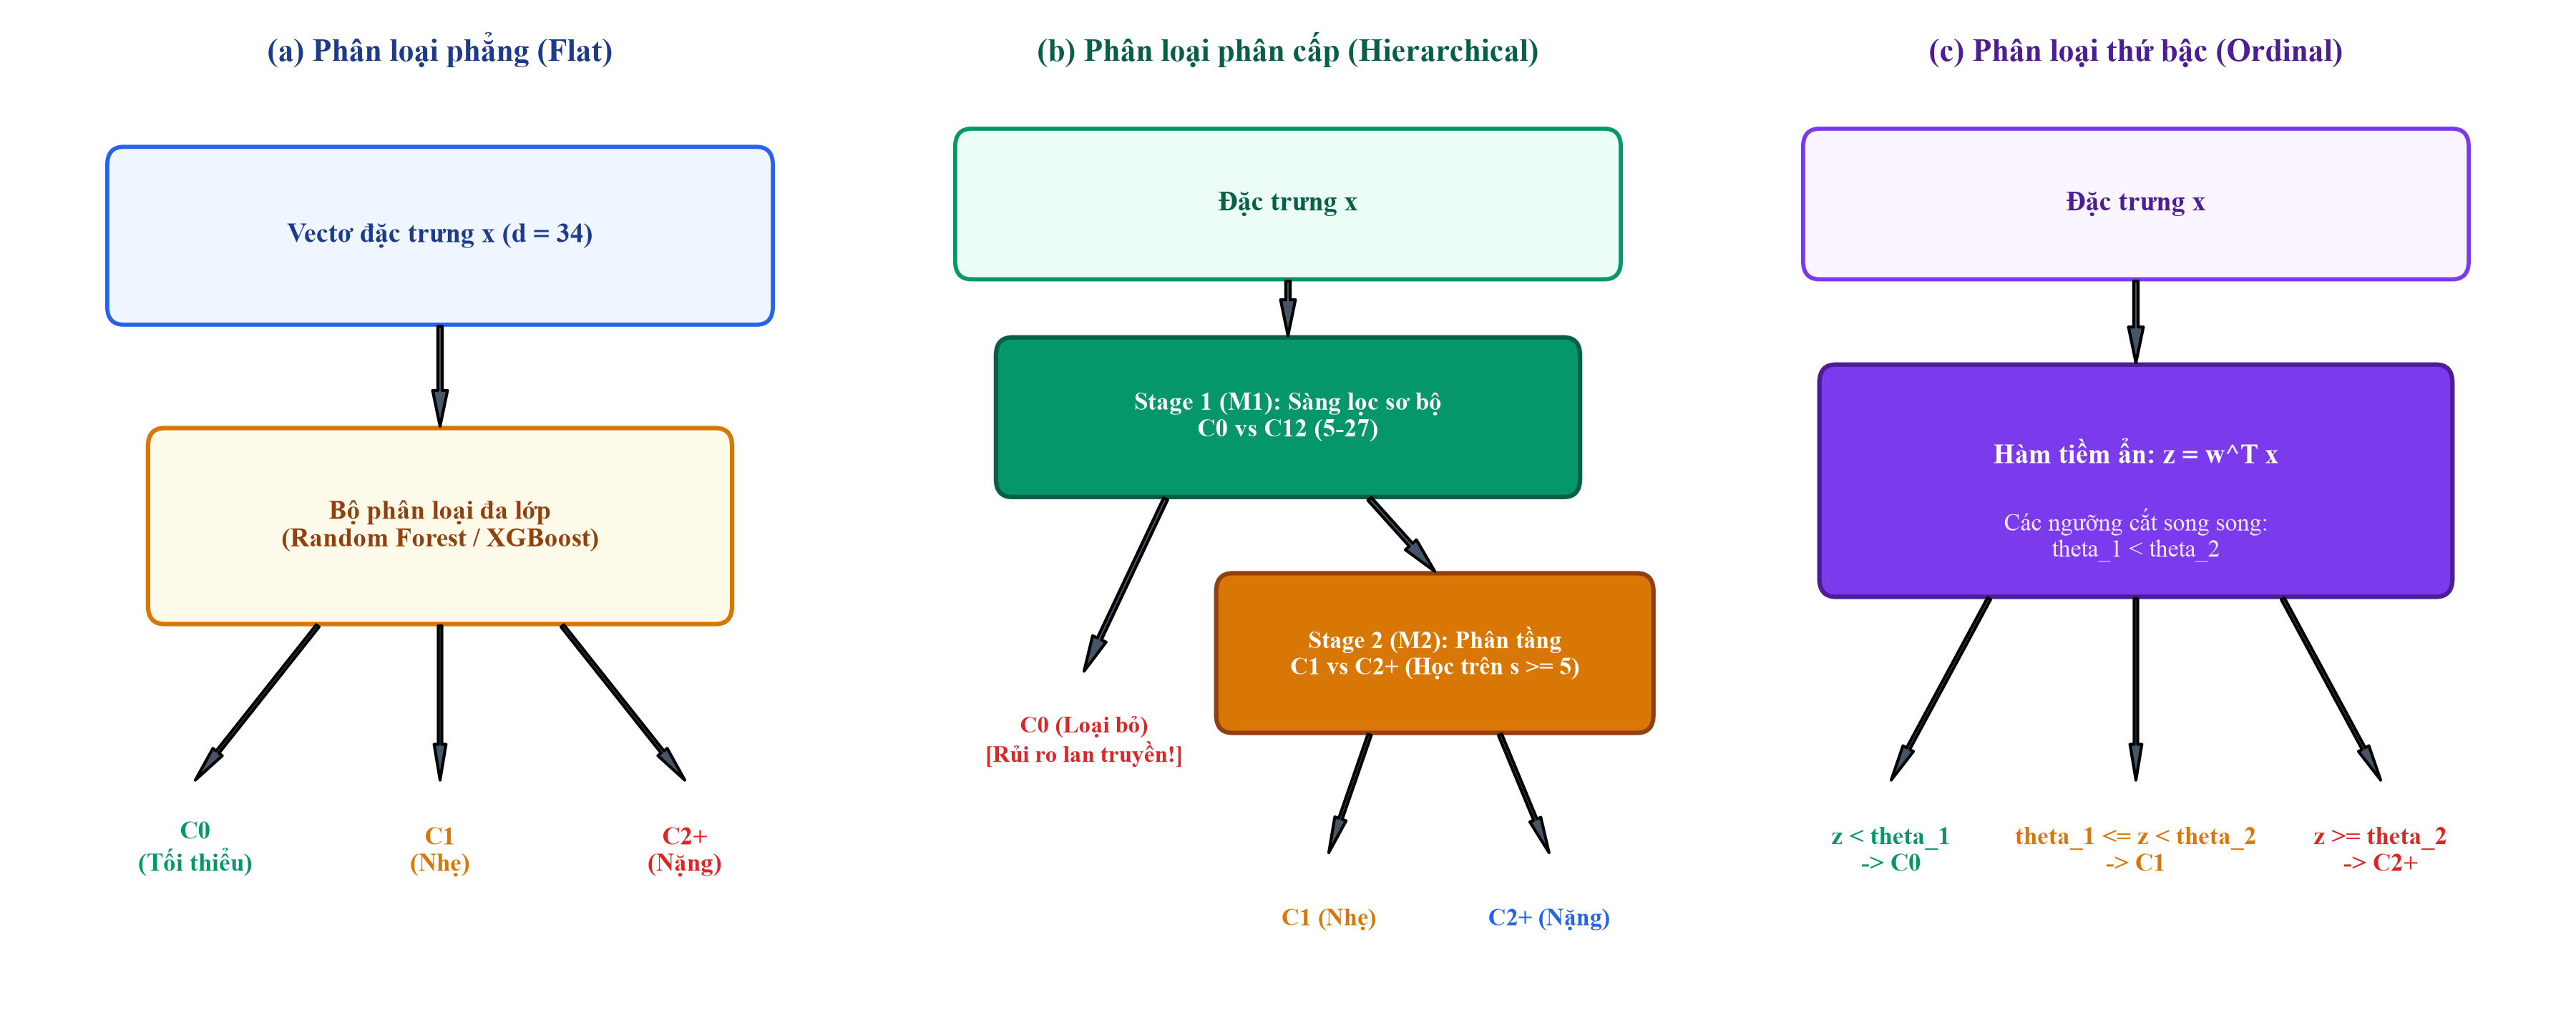
\includegraphics[width=\textwidth]{figures/fig2_modeling_paradigms.png}
\label{fig:modeling-paradigms}
\end{figure}
\FloatBarrier

\subsection{Phương pháp phân loại phẳng (Flat Classification)}
\label{subsec:flat-paradigm}

Cách tiếp cận phân loại phẳng coi $K$ mức độ nghiêm trọng là các nhãn danh nghĩa hoàn toàn độc lập. Mô hình học trực tiếp một hàm ánh xạ $f: \mathbb{R}^d \to \Delta^K$ để dự đoán phân phối xác suất hậu nghiệm $P(Y = k \mid \mathbf{x})$. Các thuật toán cơ sở gồm Logistic Regression, Random Forest và XGBoost.

Ưu điểm của phương pháp phẳng là tính trực tiếp, dễ triển khai bằng các thư viện học máy tiêu chuẩn. Tuy nhiên, đặc điểm của phương pháp này là không khai thác quan hệ thứ tự tự nhiên giữa các mức độ ($C_0 < C_1 < C_2$). Sai số nhầm lẫn giữa $C_0$ và $C_1$ (chênh 1 bậc) được đánh giá ngang bằng với sai số giữa $C_0$ và $C_2^+$ (chênh 2 bậc). Đồng thời, khi dữ liệu mất cân bằng lớn, ranh giới phân tách phẳng có xu hướng nghiêng về lớp đa số.

\subsection{Phương pháp phân loại phân cấp (Hierarchical Classification)}
\label{subsec:hierarchical-paradigm}

Nhằm mô phỏng quy trình sàng lọc hai bước (trước hết nhận diện người có triệu chứng, sau đó mới phân tầng mức độ), phương pháp phân cấp chia nhỏ bài toán thành cấu trúc gồm hai giai đoạn \cite{silla2011survey}:
\begin{itemize}
    \item \textbf{Giai đoạn 1 (Mô hình sàng lọc Stage 1):} Phân loại nhị phân giữa nhóm triệu chứng tối thiểu ($C_0$) và nhóm có triệu chứng ($C_{12} = C_1 \cup C_2^+$).
    \item \textbf{Giai đoạn 2 (Mô hình phân tầng Stage 2):} Trong số các mẫu có triệu chứng, phân biệt giữa mức độ nhẹ ($C_1$) và mức độ nặng theo quy ước ($C_2^+$).
\end{itemize}

Kiến trúc phân cấp được thử nghiệm với hai cơ chế định tuyến:
\begin{enumerate}
    \item \textbf{Định tuyến cứng (Hard Routing):} Nếu Stage 1 dự đoán một mẫu là $C_0$, mẫu đó lập tức được gán nhãn $C_0$ và kết thúc luồng. Cơ chế này dẫn đến hiện tượng \textbf{lan truyền sai số một chiều (Error Propagation)}: nếu một mẫu nặng $C_2^+$ bị Stage 1 gán nhầm thành $C_0$, sai sót này không thể sửa chữa ở Giai đoạn 2.
    \item \textbf{Định tuyến mềm (Soft Routing):} Cả hai mô hình Stage 1 và Stage 2 đều xuất ra vectơ xác suất liên tục. Xác suất hậu nghiệm toàn thể $\hat{P}(C_k \mid \mathbf{x})$ được kết hợp theo quy tắc nhân xác suất có điều kiện (chi tiết công thức được trình bày tại Mục \ref{subsec:soft-cost-hierarchical}). Cơ chế mềm bảo toàn thông tin xác suất liên tục và loại bỏ hiện tượng tắc nghẽn một chiều của định tuyến cứng.
\end{enumerate}

\subsection{Lý thuyết quyết định nhạy chi phí Bayes (Bayes Cost-Sensitive Decision)}
\label{subsec:cost-sensitive-paradigm}

Trong sàng lọc y tế, các loại sai lầm có mức độ ảnh hưởng khác nhau: việc bỏ sót một ca bệnh nặng ($C_2^+ \to C_0$) thường mang lại rủi ro lớn hơn so với một ca báo động nhầm ($C_0 \to C_2^+$). Lý thuyết quyết định nhạy chi phí Bayes \cite{elkan2001foundations} cung cấp cơ sở toán học để tối ưu quyết định dưới sự bất cân xứng này.

Quy ước ma trận chi phí $\mathbf{C} \in \mathbb{R}^{K \times K}$, trong đó phần tử $\mathbf{C}(i, j)$ là chi phí phạt khi nhãn thực tế là $i$ và nhãn dự đoán là $j$ (với $\mathbf{C}(i, i) = 0$). Rủi ro kỳ vọng được tính theo tổng xác suất nhân trọng số phạt: $R(j \mid \mathbf{x}) = \sum_{i} \hat{P}(C_i \mid \mathbf{x}) \cdot \mathbf{C}(i, j)$. Quy tắc quyết định tối ưu Bayes lựa chọn nhãn $\hat{y}^* = \arg\min_j R(j \mid \mathbf{x})$ nhằm tối thiểu hóa rủi ro kỳ vọng toàn cục. Bằng cách gán trọng số phạt lớn cho phần tử $\mathbf{C}(2, 0)$ (nhãn thật là $C_2^+$, dự đoán nhầm thành $C_0$), mô hình chủ động dịch chuyển ranh giới quyết định để bảo vệ các ca nặng (chi tiết thiết lập 4 ma trận chi phí $M_0 \dots M_3$ được trình bày tại Mục \ref{subsec:soft-cost-hierarchical} và Phụ lục \ref{app:cost-matrices}).

\subsection{Phương pháp phân loại thứ bậc (Ordinal Classification)}
\label{subsec:ordinal-paradigm}

Do các mức độ triệu chứng PHQ-9 có tính chất thứ bậc ($C_0 < C_1 < C_2^+$), phân loại thứ bậc khai thác cấu trúc trật tự này để hạn chế các sai số nhảy bậc lớn \cite{mccullagh1980regression, frank2001simple}:
\begin{enumerate}
    \item \textbf{Mô hình Ordinal Logistic Regression (OLR):} Giả định tồn tại một biến tiềm ẩn tuyến tính $z = \mathbf{w}^T \mathbf{x}$ và tập hợp các ngưỡng cắt đơn điệu $\theta_1 < \theta_2 < \dots < \theta_{K-1}$. Xác suất tích lũy được mô hình hóa theo hàm phân phối Logistic:
    \begin{equation}
        P(Y \le k \mid \mathbf{x}) = \sigma(\theta_{k+1} - \mathbf{w}^T \mathbf{x}) = \frac{1}{1 + e^{-(\theta_{k+1} - \mathbf{w}^T \mathbf{x})}}
    \end{equation}
    Mô hình OLR sử dụng chung một vectơ trọng số $\mathbf{w}$ cho tất cả các ranh giới (giả định proportional odds), giúp số lượng tham số gọn và các siêu phẳng quyết định song song không bao giờ cắt nhau.
    \item \textbf{Phân loại nhị phân tích lũy (Cumulative Binary Classification -- CBC):} Huấn luyện $K-1$ bộ phân loại nhị phân độc lập $h_k(\mathbf{x})$ để dự đoán biến cố tích lũy $P(Y \ge k \mid \mathbf{x})$. Tuy nhiên, phương pháp này tiềm ẩn nguy cơ vi phạm tính đơn điệu xác suất khi xuất hiện $P(Y \ge k+1) > P(Y \ge k)$ trên một số mẫu dữ liệu ngoài mẫu.
\end{enumerate}

\section{Tổng quan các nghiên cứu liên quan}
\label{sec:nghien-cuu-lien-quan}

Trong những năm gần đây, việc áp dụng học máy trên dữ liệu khảo sát NHANES để nghiên cứu trầm cảm đã được quan tâm trong y văn. Bảng \ref{tab:related-works} tổng hợp các công trình tiêu biểu liên quan.

\begin{table}[htbp]{Tổng hợp so sánh các nghiên cứu liên quan về dự đoán trầm cảm từ dữ liệu y tế}
\centering
\small
\setlength{\tabcolsep}{4.5pt}
\label{tab:related-works}
\begin{tabularx}{\textwidth}{p{3.2cm} p{2.2cm} p{3.2cm} X}
\toprule
\textbf{Nghiên cứu} & \textbf{Dữ liệu} & \textbf{Phương pháp} & \textbf{Kết quả \& Giới hạn chính} \\
\midrule
Pratt và cs. (2014) \cite{pratt2014depression} & NHANES 2009--2012 & Hồi quy logistic, dịch tễ & Đánh giá tỷ lệ mắc và yếu tố nguy cơ; không xây dựng mô hình học máy dự đoán. \\
\midrule
Patel và cs. (2016) \cite{patel2016systematic} & NHANES đa chu kỳ & Logistic Regression, Decision Tree & Khảo sát yếu tố nguy cơ; chỉ dừng ở bài toán nhị phân ($s \ge 10$), chưa phân tầng đa mức. \\
\midrule
Dipnall và cs. (2016) \cite{dipnall2016fusing} & NHANES 2005--2010 & Khai phá dữ liệu sinh học, GLM & Kết hợp dấu ấn sinh học; tập trung sàng lọc nhị phân, chưa khảo sát đa mức $T_3 \to T_5$. \\
\midrule
Zhang và cs. (2020) \cite{zhang2020machine} & Khảo sát cộng đồng & Random Forest, XGBoost phẳng & So sánh thuật toán dạng bảng; phân loại phẳng, chưa tối ưu chi phí cho các ca nặng. \\
\midrule
\textbf{DepSev-ML (Đề tài)} & \textbf{NHANES 3 chu kỳ} & \textbf{Random Forest, Phân cấp mềm, Chi phí Bayes, OLR} & \textbf{Khảo sát quy luật từ $T_2 \to T_5$; giảm 48.3\% ca nặng bị bỏ sót với chi phí Bayes; kiểm định ngoại suy thời gian.} \\
\bottomrule
\end{tabularx}
\end{table}

Qua khảo sát y văn, có thể rút ra một số khoảng trống nghiên cứu chính:
\begin{enumerate}
    \item Đa số các công trình trước đây tập trung vào bài toán nhị phân thô ($s \ge 10$ hoặc $s \ge 5$). Rất ít nghiên cứu khảo sát sự suy giảm hiệu năng khi mở rộng sang bài toán đa mức ($T_3 \to T_5$).
    \item Các nghiên cứu đa mức hiện có chủ yếu sử dụng mô hình phẳng truyền thống, chưa khai thác cấu trúc thứ bậc và chưa lượng hóa sự đánh đổi giữa việc giảm bỏ sót ca nặng và gia tăng báo động nhầm.
    \item Chưa có nhiều công trình đánh giá có đối chứng giữa phân cấp cứng và phân cấp mềm kết hợp tối ưu chi phí Bayes, cũng như kiểm tra tính ổn định của mô hình trên tập dữ liệu tương lai độc lập.
\end{enumerate}

\section{Tóm tắt chương}
\label{sec:tom-tat-chuong-2}

Chương 2 đã trình bày cơ sở lý thuyết về thang đo PHQ-9, các cơ chế sinh học liên quan đến triệu chứng trầm cảm, và hai thách thức chính của dữ liệu dạng bảng là mất cân bằng lớp và chồng lấn đặc trưng. Chương cũng đã phân tích chi tiết nguyên lý hoạt động của Random Forest và ba hướng tiếp cận mô hình hóa (phẳng, phân cấp, thứ bậc). Các nội dung này là cơ sở trực tiếp để xây dựng phương pháp và quy trình thực nghiệm trong Chương \ref{ch:phuong-phap}.

\chapter{Dữ liệu và phương pháp nghiên cứu}
\label{ch:phuong-phap}

Chương này trình bày chi tiết kiến trúc hệ thống, quy trình xử lý dữ liệu và thiết kế các mô hình học máy trong khung thực nghiệm \textbf{DepSev-ML}. Để trả lời các câu hỏi nghiên cứu, phương pháp luận được xây dựng dựa trên nguyên tắc module hóa, kiểm soát chặt chẽ quy trình tiền xử lý nhằm tránh rò rỉ dữ liệu, và thử nghiệm các kiến trúc phân loại từ phẳng, phân cấp đến thứ bậc.

\section{Tổng quan quy trình nghiên cứu DepSev-ML}
\label{sec:kien-truc-tong-the}

Quy trình thực nghiệm DepSev-ML được tổ chức thành 7 bước chính như mô tả trong Hình \ref{fig:overall-architecture}.

\begin{figure}[htbp]{Sơ đồ quy trình nghiên cứu thực nghiệm 7 bước của DepSev-ML}
\centering
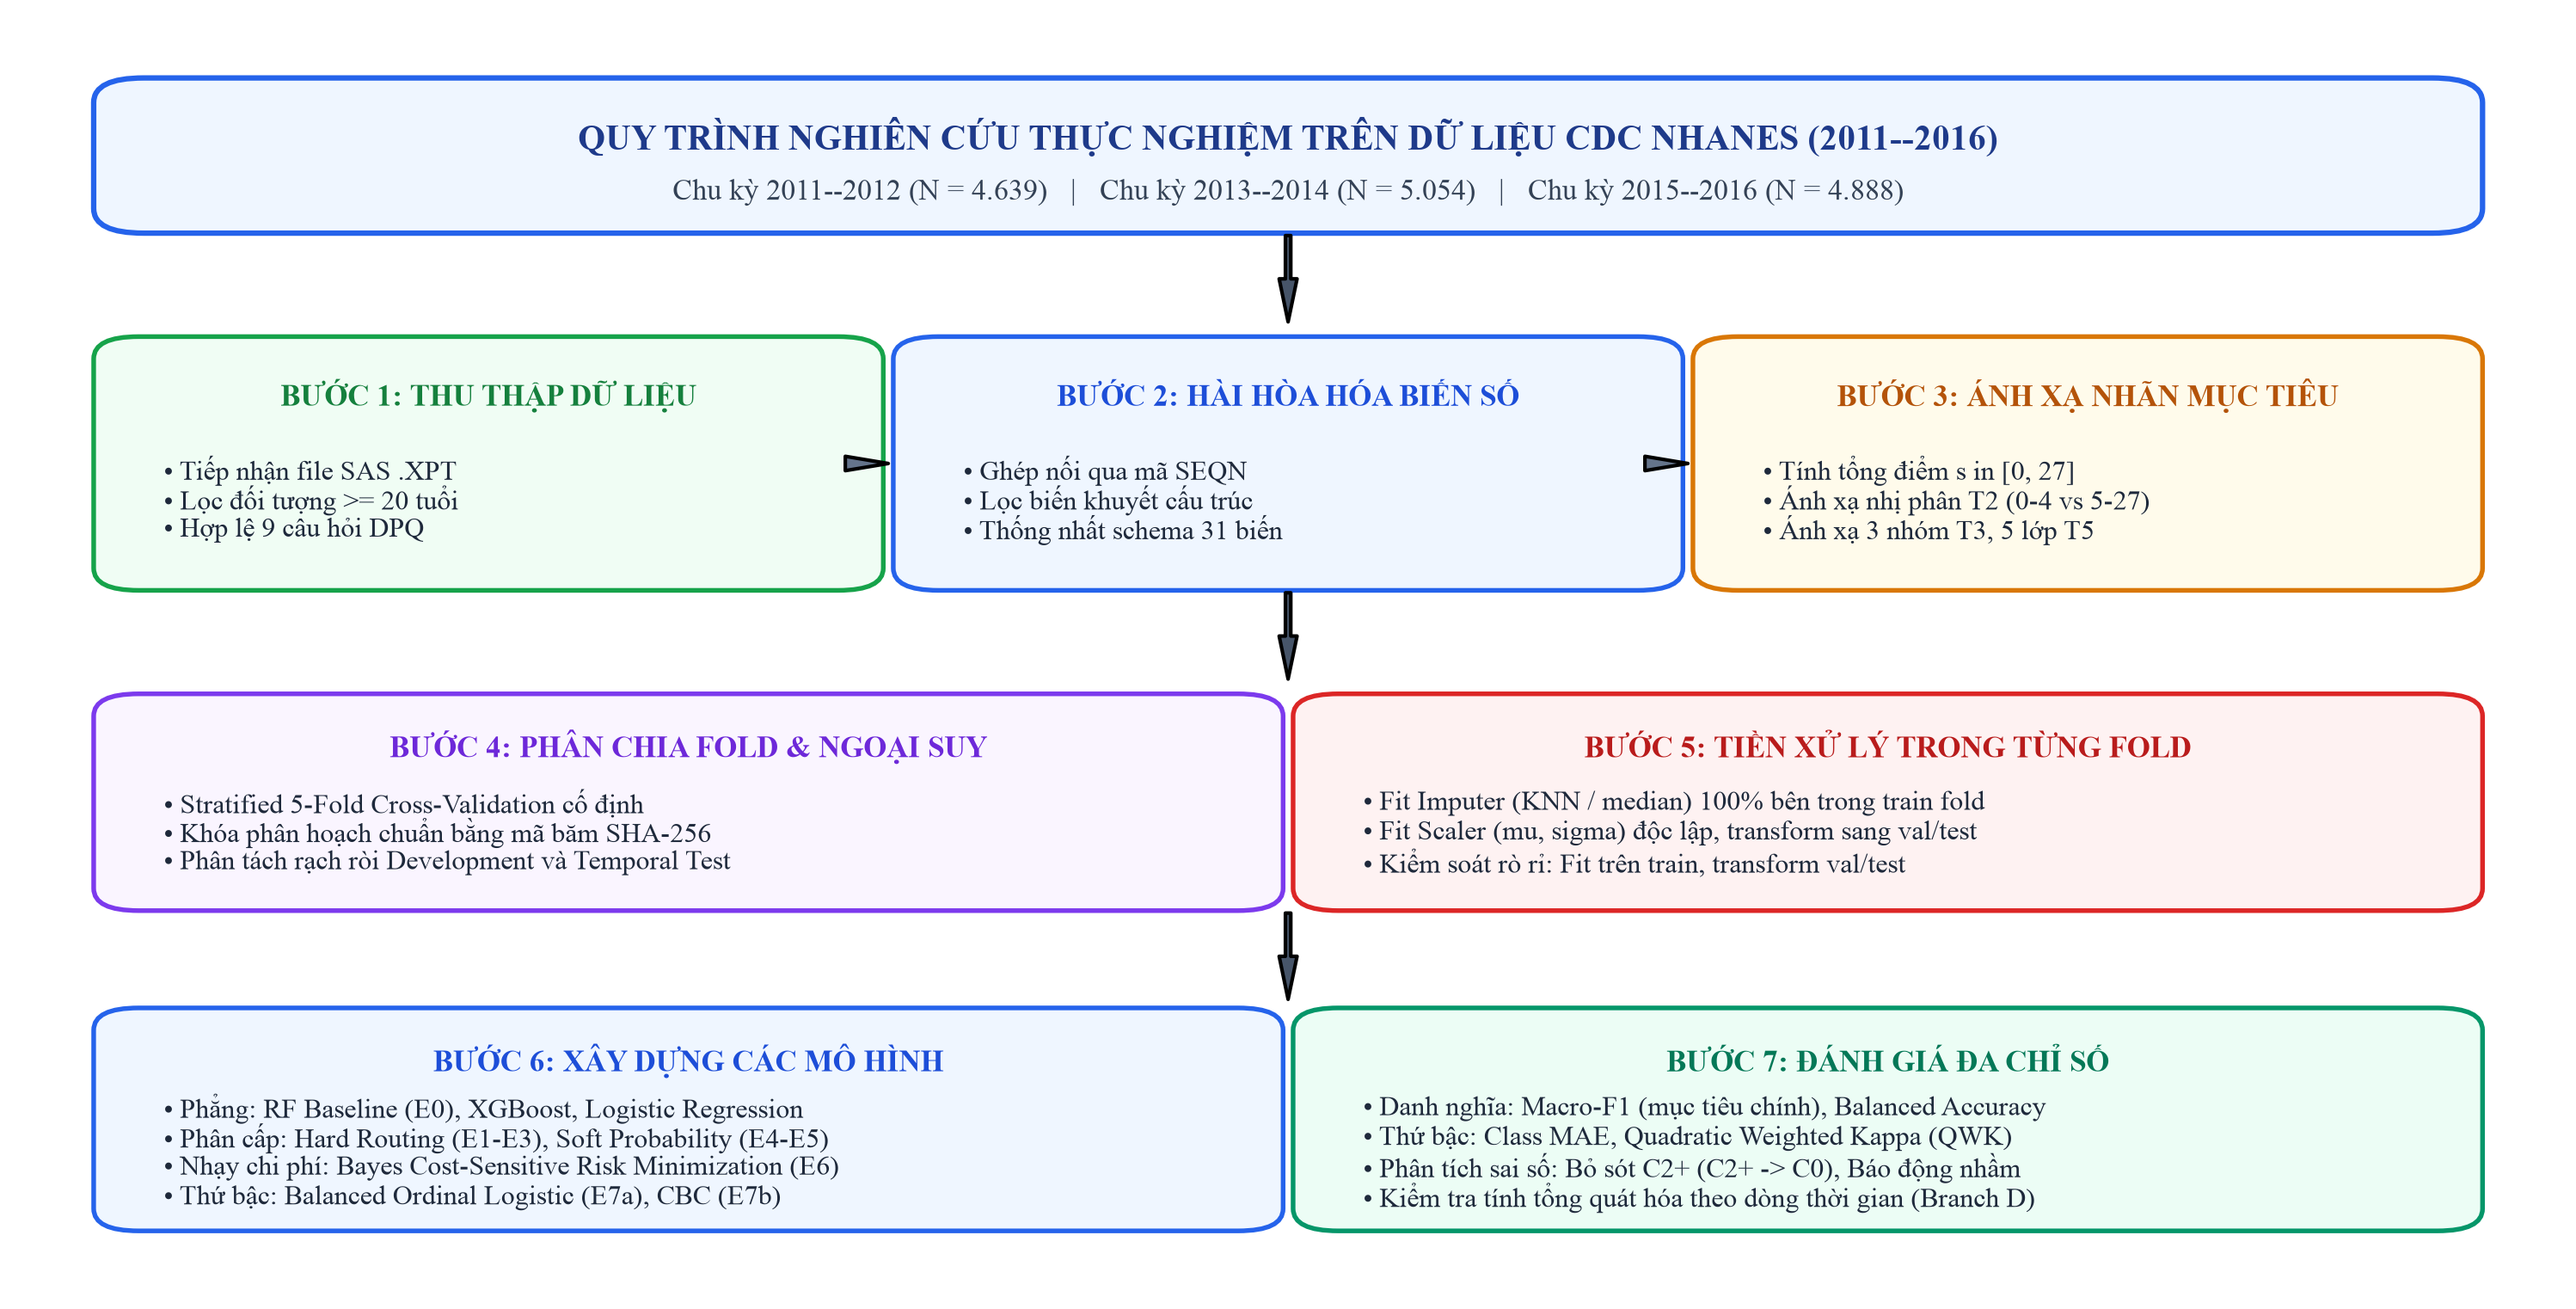
\includegraphics[width=\textwidth]{figures/depsev_overall_architecture.png}
\label{fig:overall-architecture}
\end{figure}
\FloatBarrier

Các bước thực hiện các chức năng cụ thể:
\begin{enumerate}
    \item \textbf{Bước 1 -- Tiếp nhận và lọc đối tượng (Cohort Filtering):} Tiếp nhận các tệp dữ liệu gốc định dạng SAS Transport (.XPT) từ cổng thông tin CDC/NCHS, áp dụng tiêu chuẩn chọn đối tượng người trưởng thành ($\text{RIDAGEYR} \ge 20$) có đầy đủ 9 câu hỏi khảo sát DPQ hợp lệ.
    \item \textbf{Bước 2 -- Hài hòa hóa và trích xuất đặc trưng (Feature Engineering):} Ghép nối các bảng khảo sát và xét nghiệm qua mã định danh SEQN; chuẩn hóa tên biến, xử lý biến điều hướng và loại bỏ các biến có tỷ lệ khuyết thiếu lớn giữa các chu kỳ.
    \item \textbf{Bước 3 -- Thiết lập không gian nhãn mục tiêu (Target Space Mapping):} Ánh xạ tổng điểm PHQ-9 thành 4 không gian mục tiêu rời rạc ($T_2, T_3, T_4, T_5$) phục vụ khảo sát đa độ phân giải.
    \item \textbf{Bước 4 -- Phân hoạch dữ liệu có kiểm soát (Partitioning):} Quản lý các phân hoạch dữ liệu cố định (Stratified 5-Fold CV, Development/Held-out splits) bằng mã băm SHA-256 nhằm bảo đảm tính tái lập thực nghiệm.
    \item \textbf{Bước 5 -- Tiền xử lý dữ liệu in-fold (In-Fold Preprocessing):} Thực hiện quy trình điền khuyết (median/mode), chuẩn hóa (StandardScaler) và mã hóa one-hot độc lập bên trong từng fold huấn luyện để kiểm soát rò rỉ dữ liệu.
    \item \textbf{Bước 6 -- Thử nghiệm các hướng mô hình hóa (Model Zoo):} Triển khai mô hình phân loại phẳng ($E_0$), 4 cấu hình phân cấp cứng ($E_1 \to E_3$), 4 cấu hình phân cấp mềm kết hợp tối ưu chi phí Bayes ($E_4 \to E_6$) và các cấu hình phân loại thứ bậc ($E_7$).
    \item \textbf{Bước 7 -- Đánh giá hiệu năng đa chiều (Evaluation Suite):} Đánh giá hiệu năng qua hệ thống độ đo phân loại danh nghĩa (Macro-F1, Balanced Accuracy), độ đo thứ bậc (Class MAE, Quadratic Weighted Kappa) và số lượng ca nặng bị phân loại nhầm ($C_2^+ \to C_0$).
\end{enumerate}

\section{Bộ dữ liệu NHANES và Quy trình tiền xử lý in-fold}
\label{sec:du-lieu-nghien-cuu}

\subsection{Tập dữ liệu phát triển Legacy (NHANES 2013--2014)}
\label{subsec:legacy-cohort}

Tập dữ liệu Legacy được xây dựng từ chu kỳ NHANES 2013--2014, gồm $N = 5.054$ đối tượng trưởng thành có dữ liệu PHQ-9 hợp lệ:
\begin{itemize}
    \item \textbf{Phân hoạch phát triển (Development Cohort):} Gồm $N = 4.045$ đối tượng, được sử dụng xuyên suốt cho các thực nghiệm Stratified 5-Fold CV, Feature Ablation, Nested Hyperparameter Tuning và chuỗi thực nghiệm chính $E_0 \to E_7$.
    \item \textbf{Phân hoạch kiểm tra bổ sung (Supplementary Held-out Cohort):} Gồm $N = 1.009$ đối tượng được lưu giữ riêng để tham khảo đối chứng. Cần ghi nhận tính chất lịch sử: 813 trong số 1.009 đối tượng này từng nằm trong tập phát triển ở các phiên bản tiền nghiệm, do đó tập này chỉ mang giá trị tham chiếu phụ trợ, toàn bộ kết luận khoa học cốt lõi dựa trên quy trình kiểm định chéo Stratified 5-Fold lồng nhau trên tập phát triển.
\end{itemize}

Phân bố chi tiết các mức độ triệu chứng PHQ-9 trên tập Legacy được tổng hợp trong Bảng \ref{tab:legacy-class-dist}. Tỷ lệ lớp thiểu số rất nặng $C_4$ chỉ chiếm 1.09\%, thể hiện tính chất mất cân bằng của bài toán.

\begin{table}{Phân bố các lớp triệu chứng PHQ-9 trên tập dữ liệu Legacy ($N = 5.054$)}
\centering
\footnotesize
\setlength{\tabcolsep}{3pt}
\label{tab:legacy-class-dist}
\begin{tabularx}{\textwidth}{l c >{\centering\arraybackslash}X >{\centering\arraybackslash}X >{\centering\arraybackslash}X >{\centering\arraybackslash}X >{\centering\arraybackslash}X}
\toprule
\textbf{Phân hoạch} & \textbf{Tổng $N$} & \textbf{$C_0$ (0--4)} & \textbf{$C_1$ (5--9)} & \textbf{$C_2$ (10--14)} & \textbf{$C_3$ (15--19)} & \textbf{$C_4$ (20--27)} \\
\midrule
Development & 4.045 & 3.016 (74.56\%) & 638 (15.77\%) & 243 (6.01\%) & 104 (2.57\%) & 44 (1.09\%) \\
Held-out & 1.009 & 748 (74.13\%) & 162 (16.06\%) & 60 (5.95\%) & 28 (2.78\%) & 11 (1.09\%) \\
\midrule
\textbf{Toàn bộ} & \textbf{5.054} & \textbf{3.764 (74.48\%)} & \textbf{800 (15.83\%)} & \textbf{303 (6.00\%)} & \textbf{132 (2.61\%)} & \textbf{55 (1.09\%)} \\
\bottomrule
\end{tabularx}
\end{table}

\subsection{Tập dữ liệu đa chu kỳ chính thức (Official Multi-Cycle Cohort)}
\label{subsec:multicycle-cohort}

Để kiểm tra tính ổn định trên quy mô lớn và đánh giá khả năng tổng quát hóa theo dòng thời gian, nghiên cứu tiến hành trích xuất và hài hòa hóa dữ liệu từ ba chu kỳ NHANES liên tiếp: 2011--2012, 2013--2014 và 2015--2016, nâng tổng quy mô lên $N = 14.581$ đối tượng (Bảng \ref{tab:multicycle-class-dist}).

\begin{table}{Quy mô và phân bố các lớp triệu chứng trên các chu kỳ NHANES chính thức}
\centering
\footnotesize
\setlength{\tabcolsep}{3pt}
\label{tab:multicycle-class-dist}
\begin{tabularx}{\textwidth}{l c >{\centering\arraybackslash}X >{\centering\arraybackslash}X >{\centering\arraybackslash}X >{\centering\arraybackslash}X >{\centering\arraybackslash}X}
\toprule
\textbf{Chu kỳ / Phân nhánh} & \textbf{Tổng $N$} & \textbf{$C_0$ (\%)} & \textbf{$C_1$ (\%)} & \textbf{$C_2$ (\%)} & \textbf{$C_3$ (\%)} & \textbf{$C_4$ (\%)} \\
\midrule
NHANES 2011--2012 & 4.639 & 76.12\% & 14.79\% & 5.22\% & 2.61\% & 1.27\% \\
NHANES 2013--2014 (Branch A) & 5.054 & 74.48\% & 15.83\% & 6.00\% & 2.61\% & 1.09\% \\
NHANES 2015--2016 (Branch D Test) & 4.888 & 74.65\% & 17.21\% & 5.03\% & 2.03\% & 1.08\% \\
\midrule
\textbf{Pooled 2011--2016 (Branch B)} & \textbf{14.581} & \textbf{75.06\%} & \textbf{15.96\%} & \textbf{5.42\%} & \textbf{2.41\%} & \textbf{1.15\%} \\
\bottomrule
\end{tabularx}
\end{table}

\subsection{Quy trình tiền xử lý và kiểm soát rò rỉ dữ liệu in-fold}
\label{subsec:data-pipeline}

Quy trình tiền xử lý và hài hòa hóa dữ liệu được thực hiện như trình bày trong Hình \ref{fig:data-pipeline}.

\begin{figure}[htbp]{Quy trình tiền xử lý dữ liệu in-fold và kiểm soát rò rỉ dữ liệu}
\centering
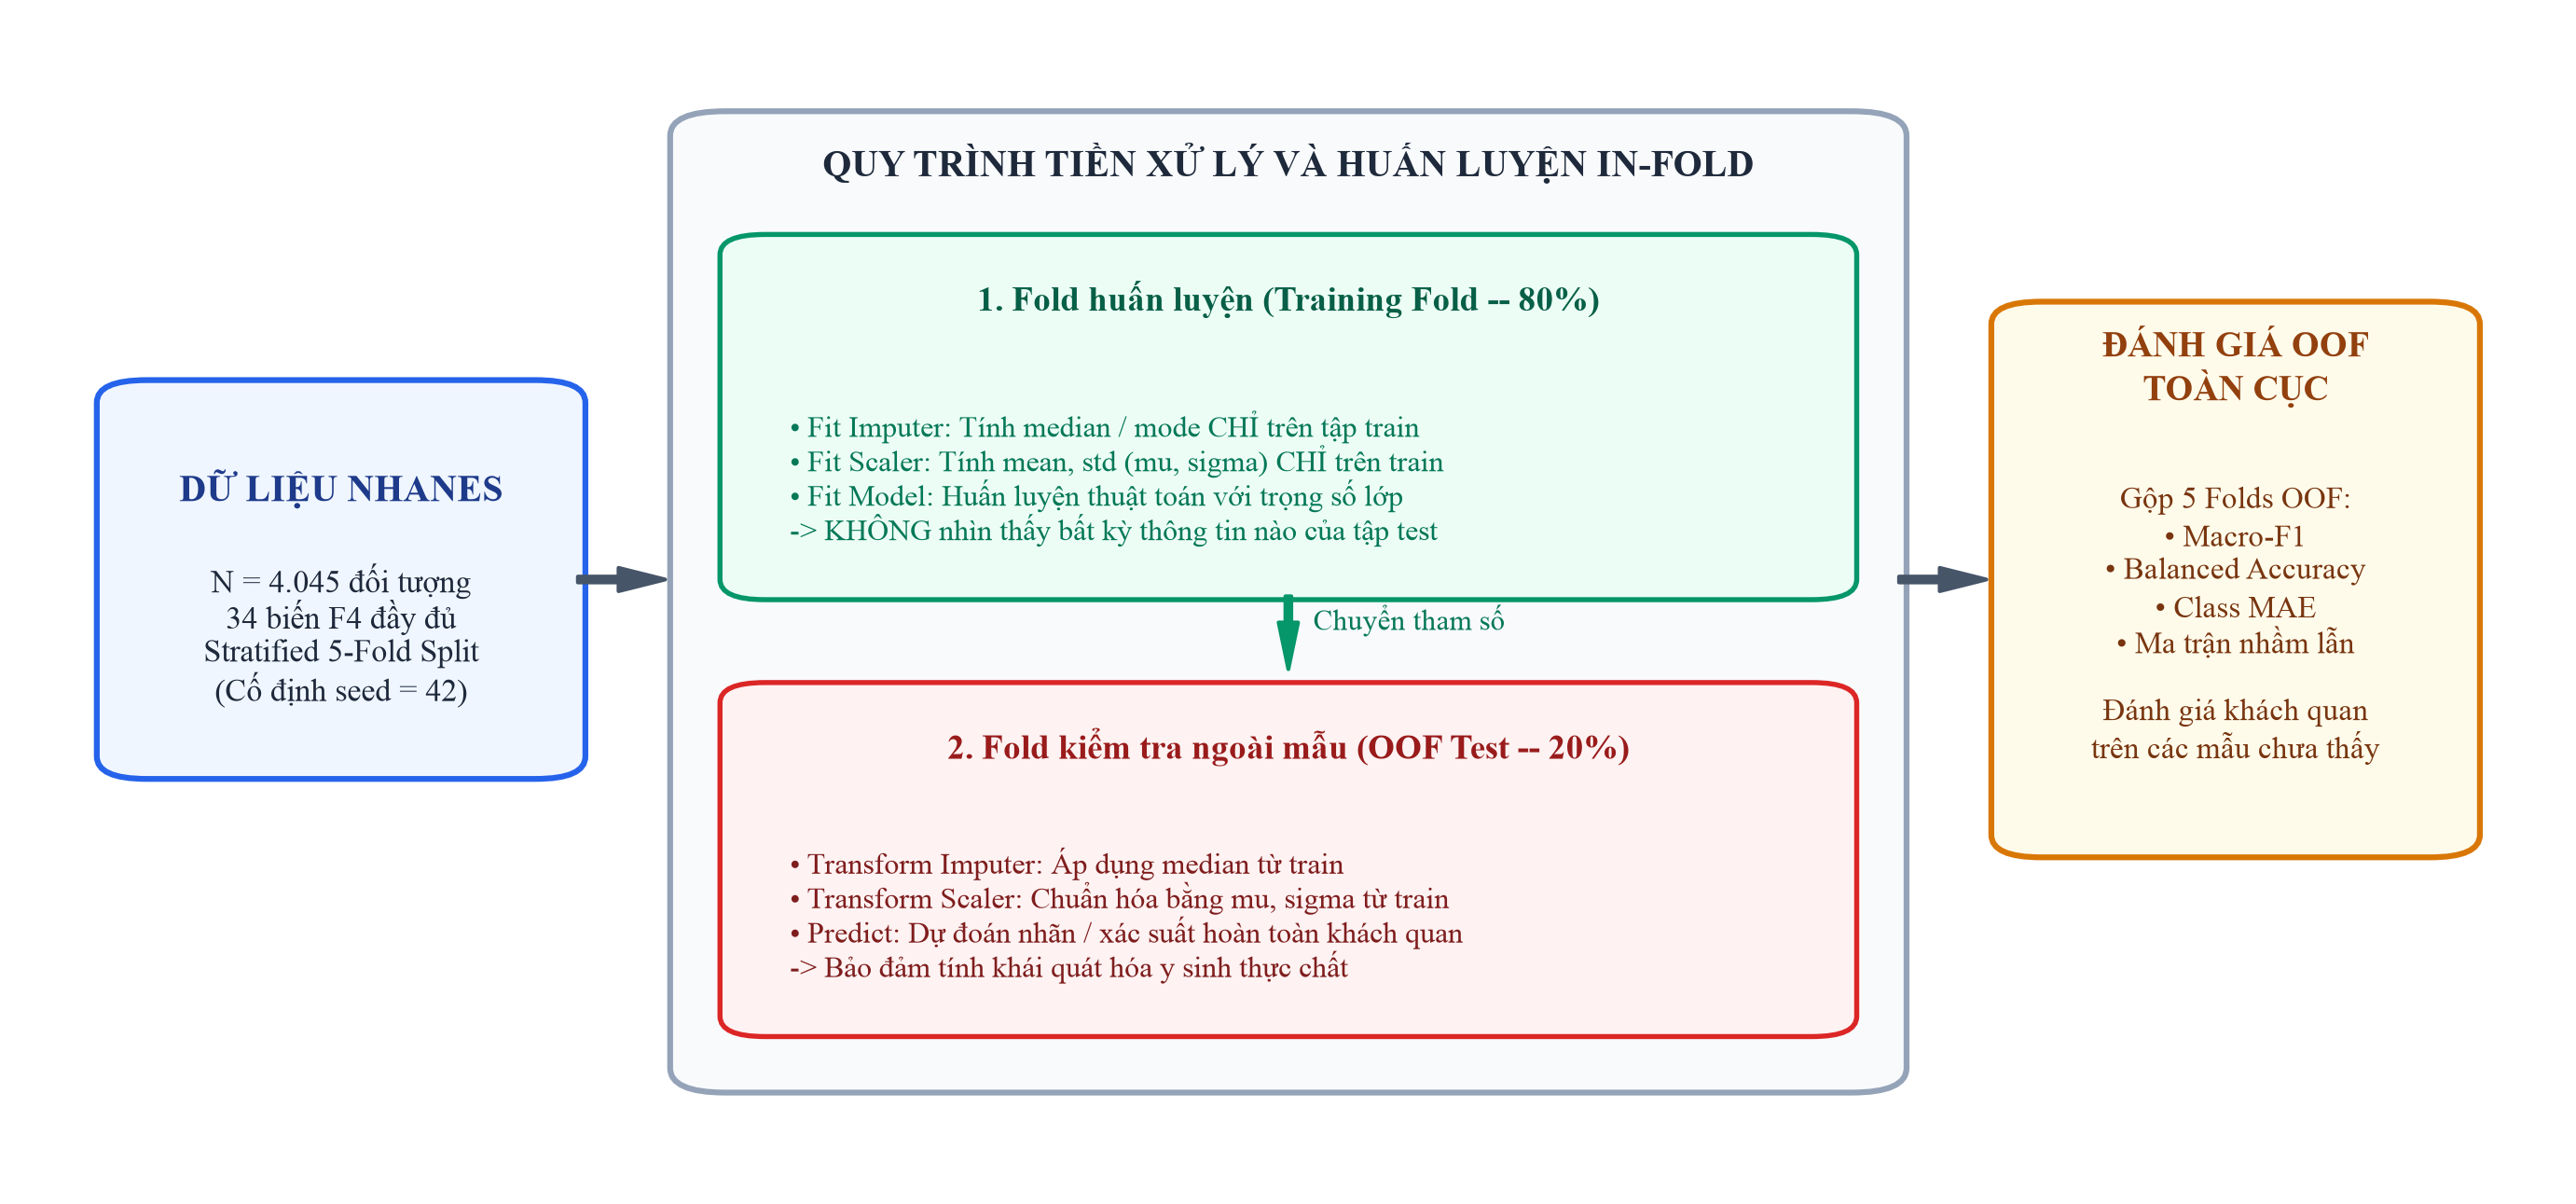
\includegraphics[width=\textwidth]{figures/fig3_infold_cv_pipeline.png}
\label{fig:data-pipeline}
\end{figure}
\FloatBarrier

Quy trình bảo đảm các yêu cầu kỹ thuật:
\begin{enumerate}
    \item \textbf{Loại trừ biến khuyết cấu trúc:} Biến xét nghiệm Triglyceride chỉ lấy mẫu trên nhóm nhịn ăn sáng ở một số chu kỳ (khuyết thiếu > 50\%), nên được loại bỏ để bảo đảm tính tương thích của 31 đặc trưng cốt lõi ($F_{4\_\text{common31}}$).
    \item \textbf{Cô lập tham số in-fold:} Các giá trị thống kê phục vụ điền khuyết (trung vị cho biến liên tục, mode cho biến phân loại) và tham số chuẩn hóa phương sai ($\mu, \sigma$ của StandardScaler) được tính độc lập trên tập huấn luyện của fold hiện tại, sau đó áp dụng biến đổi cho fold kiểm tra.
    \item \textbf{Bảo toàn nhãn mục tiêu:} Không đưa bất kỳ câu hỏi nào trong 9 mục khảo sát DPQ vào ma trận đặc trưng đầu vào $\mathbf{X}$.
\end{enumerate}

\section{Xây dựng không gian đặc trưng lũy tiến ($F_1 \to F_4$)}
\label{sec:he-thong-dac-trung}

Để khảo sát thực nghiệm mức độ đóng góp của từng nhóm biến số (RQ1), DepSev-ML tổ chức 34 biến đầu vào thành 4 không gian đặc trưng lũy tiến ($F_1 \to F_4$) như mô tả trong Hình \ref{fig:feature-groups}.

\begin{figure}[htbp]{Cấu trúc 4 không gian đặc trưng lũy tiến $F_1 \to F_4$ trong DepSev-ML}
\centering
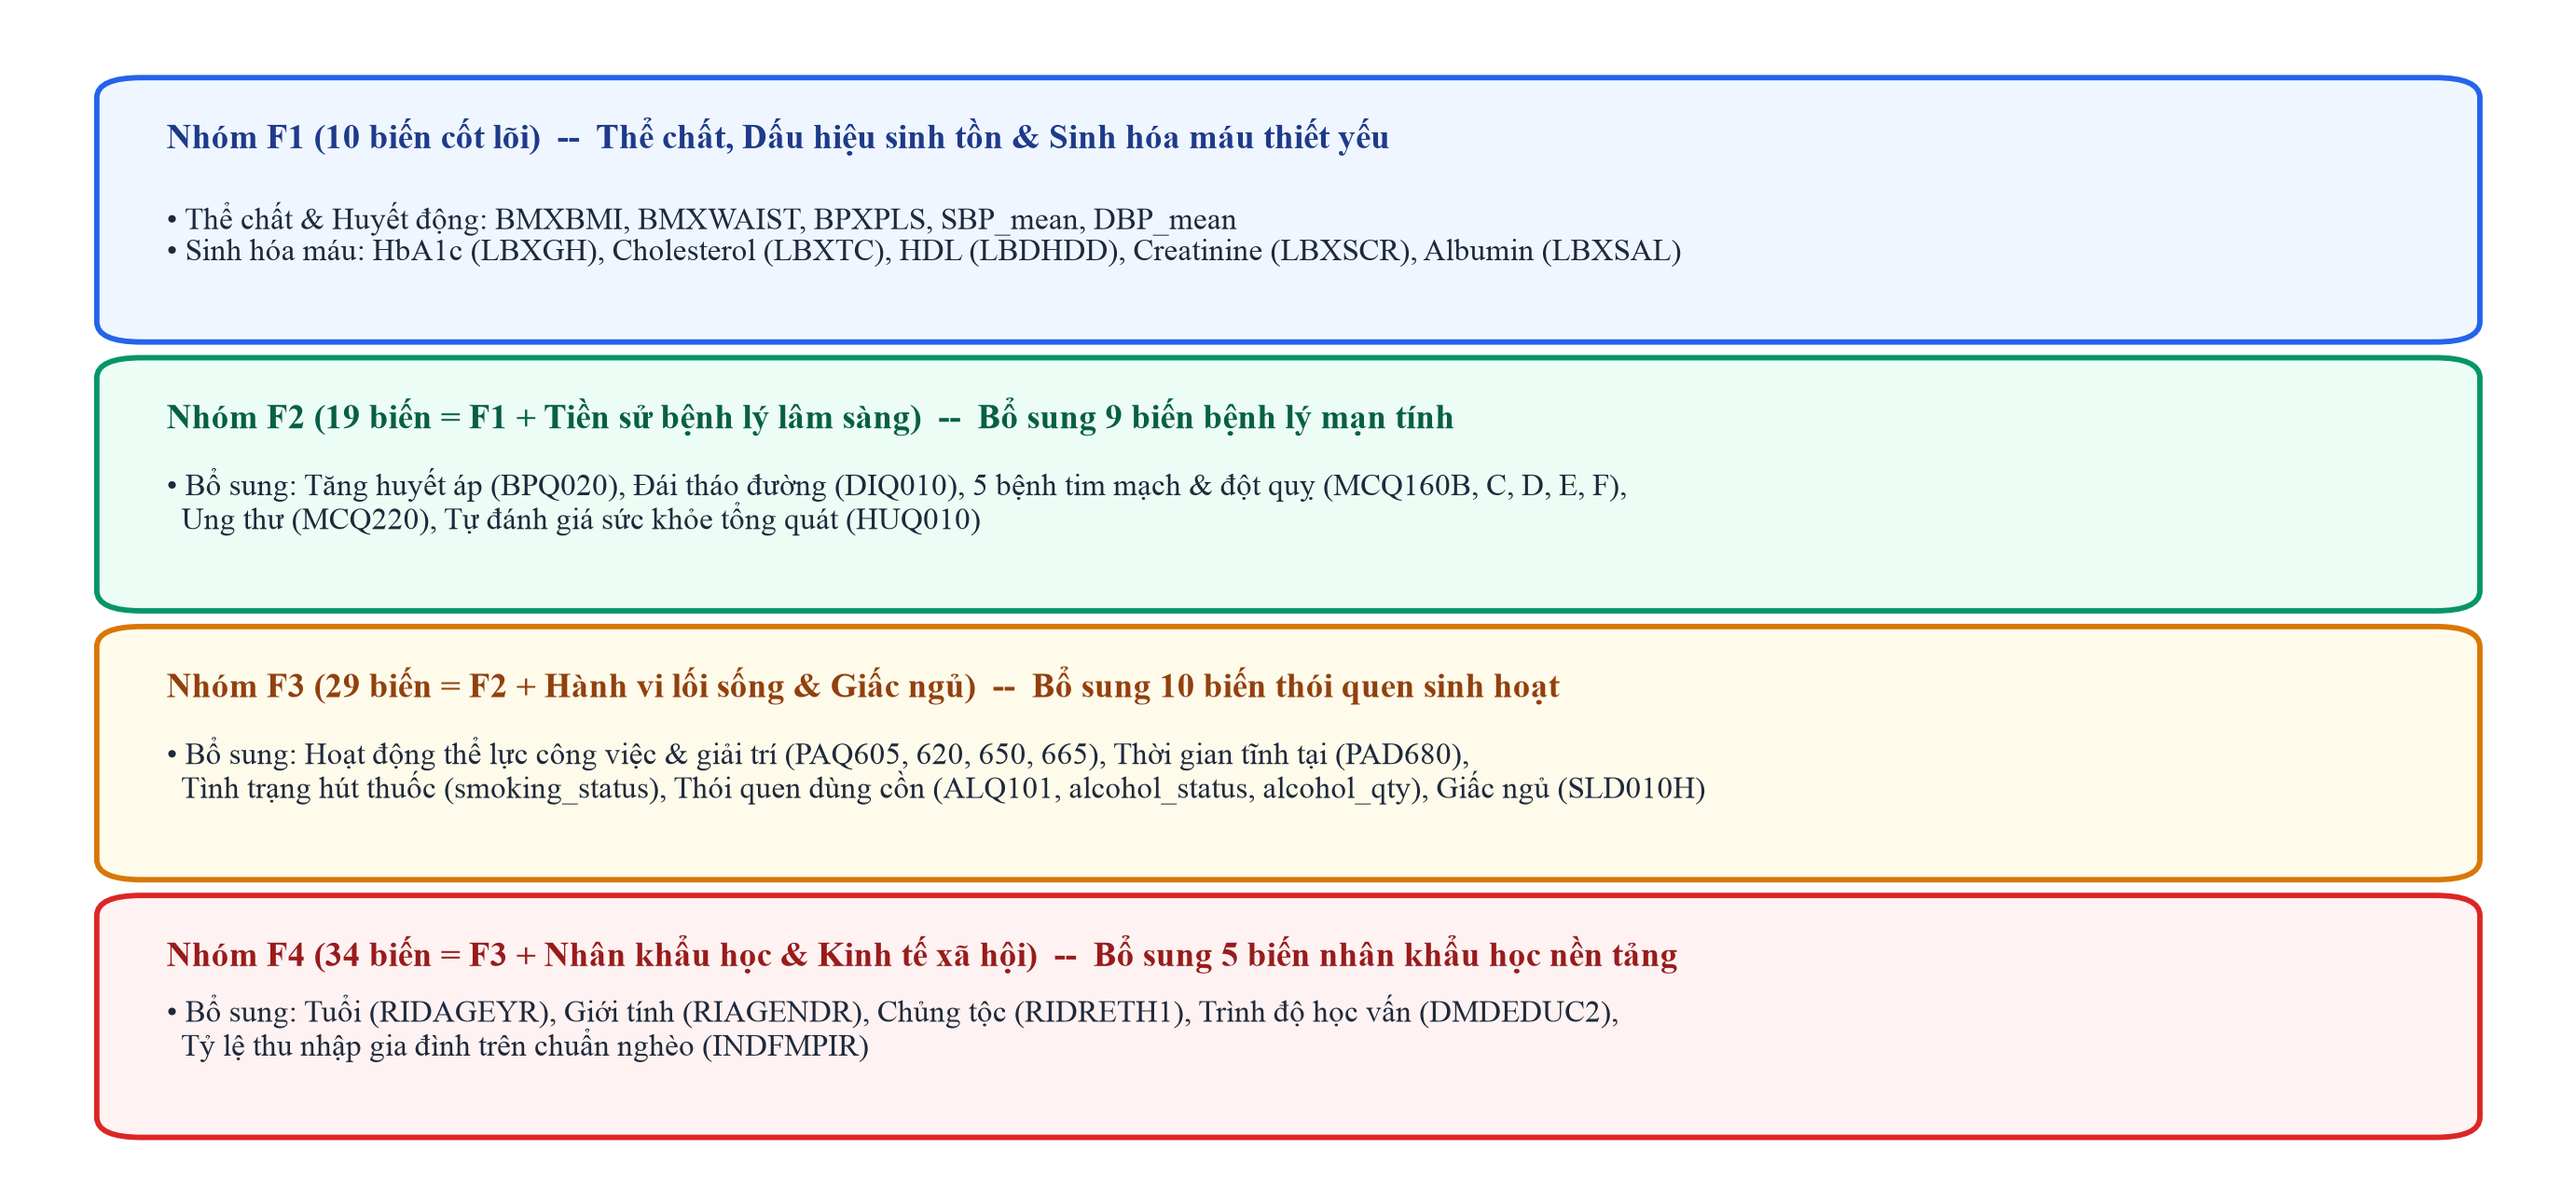
\includegraphics[width=\textwidth]{figures/fig3_3_feature_groups.png}
\label{fig:feature-groups}
\end{figure}
\FloatBarrier

Các không gian đặc trưng gồm:
\begin{itemize}
    \item \textbf{Không gian $F_1$ (10 biến cốt lõi):} Gồm 5 chỉ số thể chất và huyết áp (BMI, chu vi vòng eo, nhịp tim nghỉ, huyết áp tâm thu trung bình, huyết áp tâm trương trung bình) kết hợp 5 chỉ số sinh hóa máu (HbA1c, Cholesterol toàn phần, HDL, Creatinine và Albumin).
    \item \textbf{Không gian $F_2$ (19 biến = $F_1$ + Tiền sử bệnh lý):} Bổ sung 9 biến tiền sử bệnh mạn tính: tăng huyết áp, đái tháo đường, 5 bệnh lý tim mạch và đột quỵ, tiền sử ung thư và tự đánh giá sức khỏe.
    \item \textbf{Không gian $F_3$ (29 biến = $F_2$ + Lối sống \& Giấc ngủ):} Bổ sung 10 chỉ số hành vi: hoạt động thể lực tại nơi làm việc và giải trí, thời gian tĩnh tại, tình trạng hút thuốc, thói quen uống rượu bia và thời lượng giấc ngủ.
    \item \textbf{Không gian $F_4$ (34 biến = $F_3$ + Nhân khẩu học \& Kinh tế xã hội):} Bổ sung 5 biến nhân khẩu học: tuổi, giới tính, chủng tộc, học vấn và tỷ lệ thu nhập gia đình trên chuẩn nghèo (INDFMPIR).
\end{itemize}

Bảng \ref{tab:feature-summary} tóm tắt cấu trúc phân nhóm đặc trưng; danh mục chi tiết 34 biến kèm mã định danh CDC được trình bày tại Phụ lục \ref{app:feature-inventory}.

\begin{table}{Tóm tắt cấu trúc 4 không gian đặc trưng lũy tiến trong DepSev-ML}
\centering
\footnotesize
\setlength{\tabcolsep}{4pt}
\label{tab:feature-summary}
\begin{tabularx}{\textwidth}{l c p{5.5cm} X}
\toprule
\textbf{Không gian} & \textbf{Số biến} & \textbf{Các nhóm biến thành phần} & \textbf{Ý nghĩa lâm sàng và dịch tễ học} \\
\midrule
$F_1$ & 10 & Thể chất, Sinh tồn \& Xét nghiệm máu thiết yếu & Phản ánh chuyển hóa cơ bản, huyết động và viêm mạn tính \\
$F_2$ & 19 & $F_1$ + 9 tiền sử bệnh lý mạn tính & Tích hợp chẩn đoán tiền sử của bác sĩ và tự đánh giá sức khỏe \\
$F_3$ & 29 & $F_2$ + 10 hành vi lối sống \& giấc ngủ & Bổ sung nhịp sinh học, mức độ vận động và hành vi kích thích \\
$F_4$ & 34 & $F_3$ + 5 nhân khẩu học \& kinh tế xã hội & Bổ sung yếu tố nguy cơ xã hội, độ tuổi và áp lực kinh tế \\
\midrule
$F_{4\_\text{common31}}$ & 31 & 31 biến đồng nhất trên cả 3 chu kỳ NHANES & Chuẩn hóa schema phục vụ kiểm định đa chu kỳ Pooled \\
\bottomrule
\end{tabularx}
\end{table}

\section{Xây dựng nhãn PHQ-9 và các không gian mục tiêu ($T_2 \to T_5$)}
\label{sec:nhan-muc-tieu}

Từ tổng điểm PHQ-9 liên tục $s \in [0, 27]$, nghiên cứu thiết lập 4 không gian phân loại mục tiêu:
\begin{itemize}
    \item $T_2$ ($K=2$): Nhị phân giữa $C_0$ ($s \in [0, 4]$) và nhóm có triệu chứng ($s \in [5, 27]$).
    \item $T_3$ ($K=3$): Ba nhóm gộp quy ước gồm $C_0$ ($0$--$4$, 74.6\%), $C_1$ ($5$--$9$, 15.8\%) và $C_2^+$ ($10$--$27$, 9.7\%). Nhóm $C_2^+$ được quy ước là "nhóm Nặng theo quy ước nghiên cứu" (Severe convention) bao gồm toàn bộ các ca từ Moderate đến Severe chuẩn.
    \item $T_4$ ($K=4$): Bốn mức gồm $C_0$ ($0$--$4$), $C_1$ ($5$--$9$), $C_2$ ($10$--$14$), và $C_3^+$ ($15$--$27$).
    \item $T_5$ ($K=5$): Năm mức độ lâm sàng chuẩn PHQ-9 gồm $C_0$ (Minimal), $C_1$ (Mild), $C_2$ (Moderate), $C_3$ (Moderately severe), và $C_4$ (Severe).
\end{itemize}

\section{Quy trình áp dụng Random Forest trên dữ liệu thực tế NHANES}
\label{sec:xay-dung-random-forest}

Random Forest đóng vai trò là mô hình học máy cơ sở chính trong toàn bộ khung nghiên cứu DepSev-ML. Quy trình phát triển, huấn luyện và kiểm định mô hình Random Forest trên dữ liệu NHANES gồm các bước:

\begin{enumerate}
    \item \textbf{Bước 1 -- Xác lập tập dữ liệu và không gian đặc trưng:} 
    Mô hình được áp dụng trên tập dữ liệu phát triển Legacy gồm $N = 4.045$ đối tượng với không gian 34 đặc trưng đầy đủ ($F_4$). Phân phối nhãn 5 lớp mất cân bằng rõ rệt: $C_0$ chiếm $3.016$ ca (74.56\%), $C_1$ chiếm $638$ ca (15.77\%), $C_2$ chiếm $243$ ca (6.01\%), $C_3$ chiếm $104$ ca (2.57\%) và $C_4$ chỉ có $44$ ca (1.09\%).
    
    \item \textbf{Bước 2 -- Thiết lập phân hoạch Stratified 5-Fold Cross-Validation:} 
    Dữ liệu được phân chia thành 5 folds bằng cơ chế Stratified cố định hạt giống ngẫu nhiên \textnormal{random\_state = 42}, bảo đảm tỷ lệ giữa các lớp nhãn tương đồng giữa tập huấn luyện (4 folds, $\approx 3.236$ mẫu) và tập kiểm định (1 fold, $\approx 809$ mẫu). Cấu trúc kiểm định lồng nhau (Nested CV: Outer 5 folds, Inner 3 folds) được thiết lập để tìm kiếm siêu tham số mà không tiếp xúc với tập kiểm tra của fold ngoài.
    
    \item \textbf{Bước 3 -- Thực hiện tiền xử lý in-fold kiểm soát rò rỉ dữ liệu:} 
    Để kiểm soát nguy cơ rò rỉ dữ liệu (Hình \ref{fig:data-pipeline}), quy trình điền khuyết giá trị thiếu (median cho biến liên tục, mode cho biến phân loại) và chuẩn hóa phân phối (StandardScaler) được tính toán độc lập bên trong từng fold huấn luyện, sau đó áp dụng lên fold kiểm định.
    
    \item \textbf{Bước 4 -- Cấu hình siêu tham số cố định (Frozen RF Spec):} 
    Bộ tham số thu được từ Nested CV được cố định: \textnormal{n\_estimators = 150, max\_depth = 8, max\_features = 0.5, min\_samples\_split = 10, min\_samples\_leaf = 8, criterion = 'gini', random\_state = 42}. Tham số \textnormal{class\_weight = 'balanced\_subsample'} được kích hoạt để tự động điều chỉnh trọng số nghịch đảo tần số lớp trên từng mẫu bootstrap riêng biệt của mỗi cây.
    
    \item \textbf{Bước 5 -- Huấn luyện và suy luận Soft Voting:} 
    Tập hợp $150$ cây quyết định được huấn luyện độc lập trên các tập con bootstrap. Khi suy luận trên fold kiểm định, mẫu dữ liệu được đưa qua toàn bộ $150$ cây và xuất ra phân phối xác suất trung bình liên tục (Soft Voting): $\bar{P}(Y = k \mid \mathbf{x}) = \frac{1}{150}\sum_{b=1}^{150} P_b(Y = k \mid \mathbf{x})$.
    
    \item \textbf{Bước 6 -- Đánh giá hiệu năng và phân tích đặc điểm ranh giới:} 
    Mô hình được đánh giá qua các chỉ số: Macro-F1, Balanced Accuracy, Weighted-F1, Brier Score và Class MAE. Kết quả thực nghiệm chi tiết của Random Forest trên bài toán 5 lớp $T_5$, phân tích ma trận nhầm lẫn và sự phân bố dự đoán giữa các lớp sẽ được trình bày tại Chương \ref{ch:thuc-nghiem}. Các đặc tính ranh giới quan sát được trên $T_5$ là cơ sở thực nghiệm để nghiên cứu mở rộng khảo sát sang các cấu trúc phân loại phân cấp và thứ bậc trên $T_3$.
\end{enumerate}

\section{Thiết kế các kiến trúc phân loại phân cấp hai giai đoạn ($T_3$) và các mô hình mở rộng ($E_0 \to E_7$)}
\label{sec:thiet-ke-kien-truc-mo-hinh}

Bên cạnh bài toán phân loại đa mức phẳng $T_5$, nghiên cứu mở rộng khảo sát sang không gian 3 nhóm ($T_3$: $C_0, C_1, C_2^+$) nhằm tìm hiểu hiệu năng và đặc điểm của các hướng tiếp cận mô hình hóa khác nhau ($E_0 \to E_7$).

\subsection{Mô hình phân loại phẳng cơ sở ($E_0$)}
\label{subsec:e0-flat}

Mô hình $E_0$ sử dụng thuật toán Random Forest đa lớp truyền thống làm đường cơ sở đối chuẩn trên không gian 3 nhóm ($C_0, C_1, C_2^+$). Dự đoán đầu ra là lớp có xác suất hậu nghiệm cực đại: $\hat{y} = \arg\max_k P(Y=k \mid \mathbf{x})$.

\subsection{Kiến trúc phân loại phân cấp hai giai đoạn định tuyến cứng ($E_1 \to E_3$)}
\label{subsec:hard-hierarchical}

Kiến trúc phân cấp hai giai đoạn phân rã bài toán 3 lớp thành hai bộ phân loại nhị phân nối tiếp (Hình \ref{fig:hard-hierarchical}):
\begin{itemize}
    \item \textbf{Giai đoạn 1 (Mô hình sàng lọc Stage 1):} Phân loại nhị phân phát hiện đối tượng có triệu chứng, phân biệt giữa nhóm triệu chứng tối thiểu ($C_0$, điểm PHQ-9 $0$--$4$) và nhóm có triệu chứng ($C_{12} = C_1 \cup C_2^+$, điểm PHQ-9 $5$--$27$).
    \item \textbf{Giai đoạn 2 (Mô hình phân tầng Stage 2):} Trong số các đối tượng có triệu chứng, tiếp tục phân biệt giữa mức độ nhẹ ($C_1$, điểm PHQ-9 $5$--$9$) và mức độ nặng theo quy ước nghiên cứu ($C_2^+$, điểm PHQ-9 $10$--$27$).
\end{itemize}

\begin{figure}[htbp]{Kiến trúc phân loại phân cấp định tuyến cứng hai giai đoạn và cơ chế lan truyền sai số}
\centering
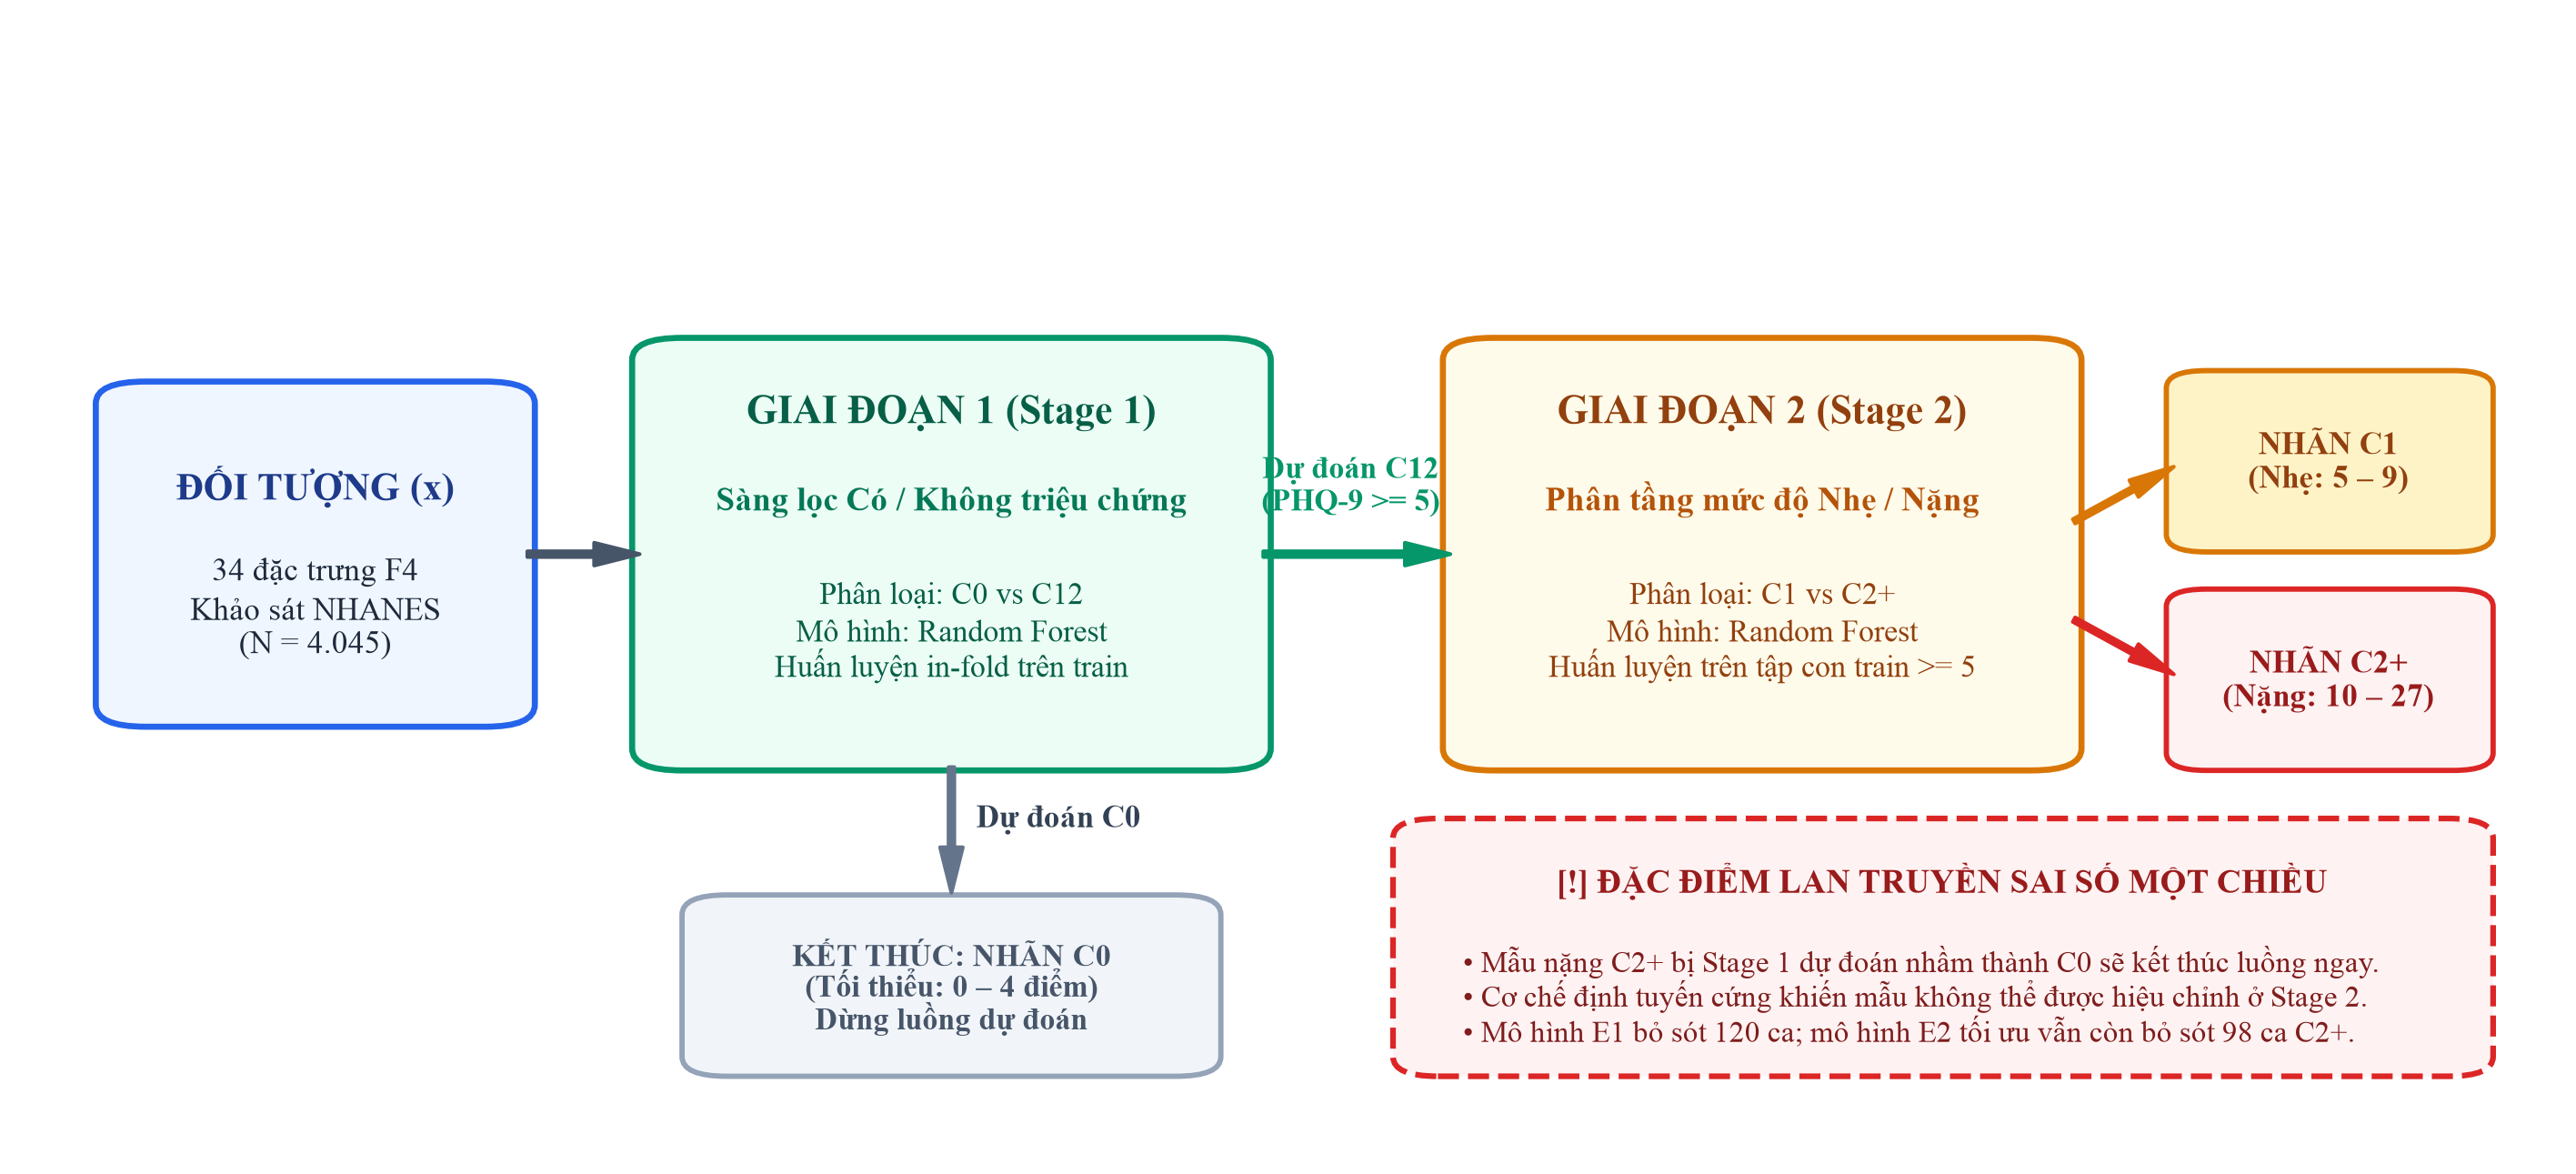
\includegraphics[width=\textwidth]{figures/fig3_4_hard_hierarchical.png}
\label{fig:hard-hierarchical}
\end{figure}
\FloatBarrier

\textbf{Quy trình huấn luyện trong từng fold của Nested Cross-Validation:}
\begin{itemize}
    \item \textbf{Mô hình Stage 1:} Trong mỗi fold kiểm định chéo, mô hình Stage 1 được huấn luyện trên \textbf{toàn bộ phần dữ liệu huấn luyện của fold đó} ($\approx 3.236$ mẫu trong số tổng $N = 4.045$ mẫu của tập phát triển).
    \item \textbf{Mô hình Stage 2:} Mô hình Stage 2 được huấn luyện \textbf{chỉ trên các mẫu trong fold huấn luyện có nhãn thật $\text{PHQ-9} \ge 5$} ($\approx 823$ mẫu trong số tổng $1.029$ mẫu có triệu chứng của tập phát triển). Việc giới hạn tập huấn luyện này giúp mô hình Stage 2 học ranh giới phân biệt giữa ca nhẹ và ca nặng mà không bị chi phối bởi lớp đa số $C_0$.
\end{itemize}

\noindent\textbf{Lưu ý về bản chất độc lập của các mô hình và bài toán:} Cần lưu ý rằng mô hình Random Forest trong bài toán 5 lớp phẳng $T_5$, mô hình RF Stage 1 trong $T_3$ và mô hình RF Stage 2 trong $T_3$ là \textbf{các mô hình độc lập, giải quyết các mục tiêu khác nhau và huấn luyện trên các tập dữ liệu khác nhau}. Đồng thời, bài toán $T_3$ là một bài toán phân loại độc lập với không gian nhãn được tái cấu trúc, không phải là kết quả cải thiện trực tiếp trên cùng không gian 5 lớp.

Bốn cấu hình thực nghiệm phân cấp cứng được khảo sát:
\begin{itemize}
    \item $E_1$: Cấu hình Random Forest nối tiếp (RF--RF) với siêu tham số mặc định.
    \item $E_2$: Cấu hình RF--RF tối ưu hóa siêu tham số và ngưỡng cắt độc lập trên từng giai đoạn.
    \item $E_{3a}$: Cấu hình kết hợp RF--LR (Stage 1 dùng RF, Stage 2 dùng Logistic Regression) để kiểm tra mô hình tuyến tính trong không gian mẫu có triệu chứng.
    \item $E_{3b}$: Cấu hình kết hợp RF--XGBoost (Stage 1 dùng RF, Stage 2 dùng XGBoost) nhằm khảo sát khả năng tăng cường độ dốc trên các ca có triệu chứng.
\end{itemize}

\textbf{Cơ chế lan truyền sai số (Error Propagation):} Do quyết định ở Giai đoạn 1 là quyết định cứng, các mẫu thuộc nhóm nặng $C_2^+$ nếu bị Stage 1 dự đoán là $C_0$ sẽ kết thúc luồng dự đoán ngay tại Stage 1 và không được Stage 2 xem xét. Đây là đặc điểm cơ học cần lưu ý khi áp dụng định tuyến cứng.

\subsection{Kiến trúc phân loại phân cấp định tuyến mềm và tối ưu chi phí Bayes ($E_4 \to E_6$)}
\label{subsec:soft-cost-hierarchical}

Nhằm tận dụng đầy đủ thông tin xác suất liên tục giữa các giai đoạn và cho phép điều chỉnh linh hoạt quy tắc quyết định, kiến trúc phân cấp mềm (Hình \ref{fig:soft-cost-architecture}) chuyển toàn bộ quá trình ra quyết định sang miền xác suất toàn phần.

\begin{figure}[htbp]{Kiến trúc phân loại phân cấp mềm kết hợp lý thuyết quyết định nhạy chi phí Bayes}
\centering
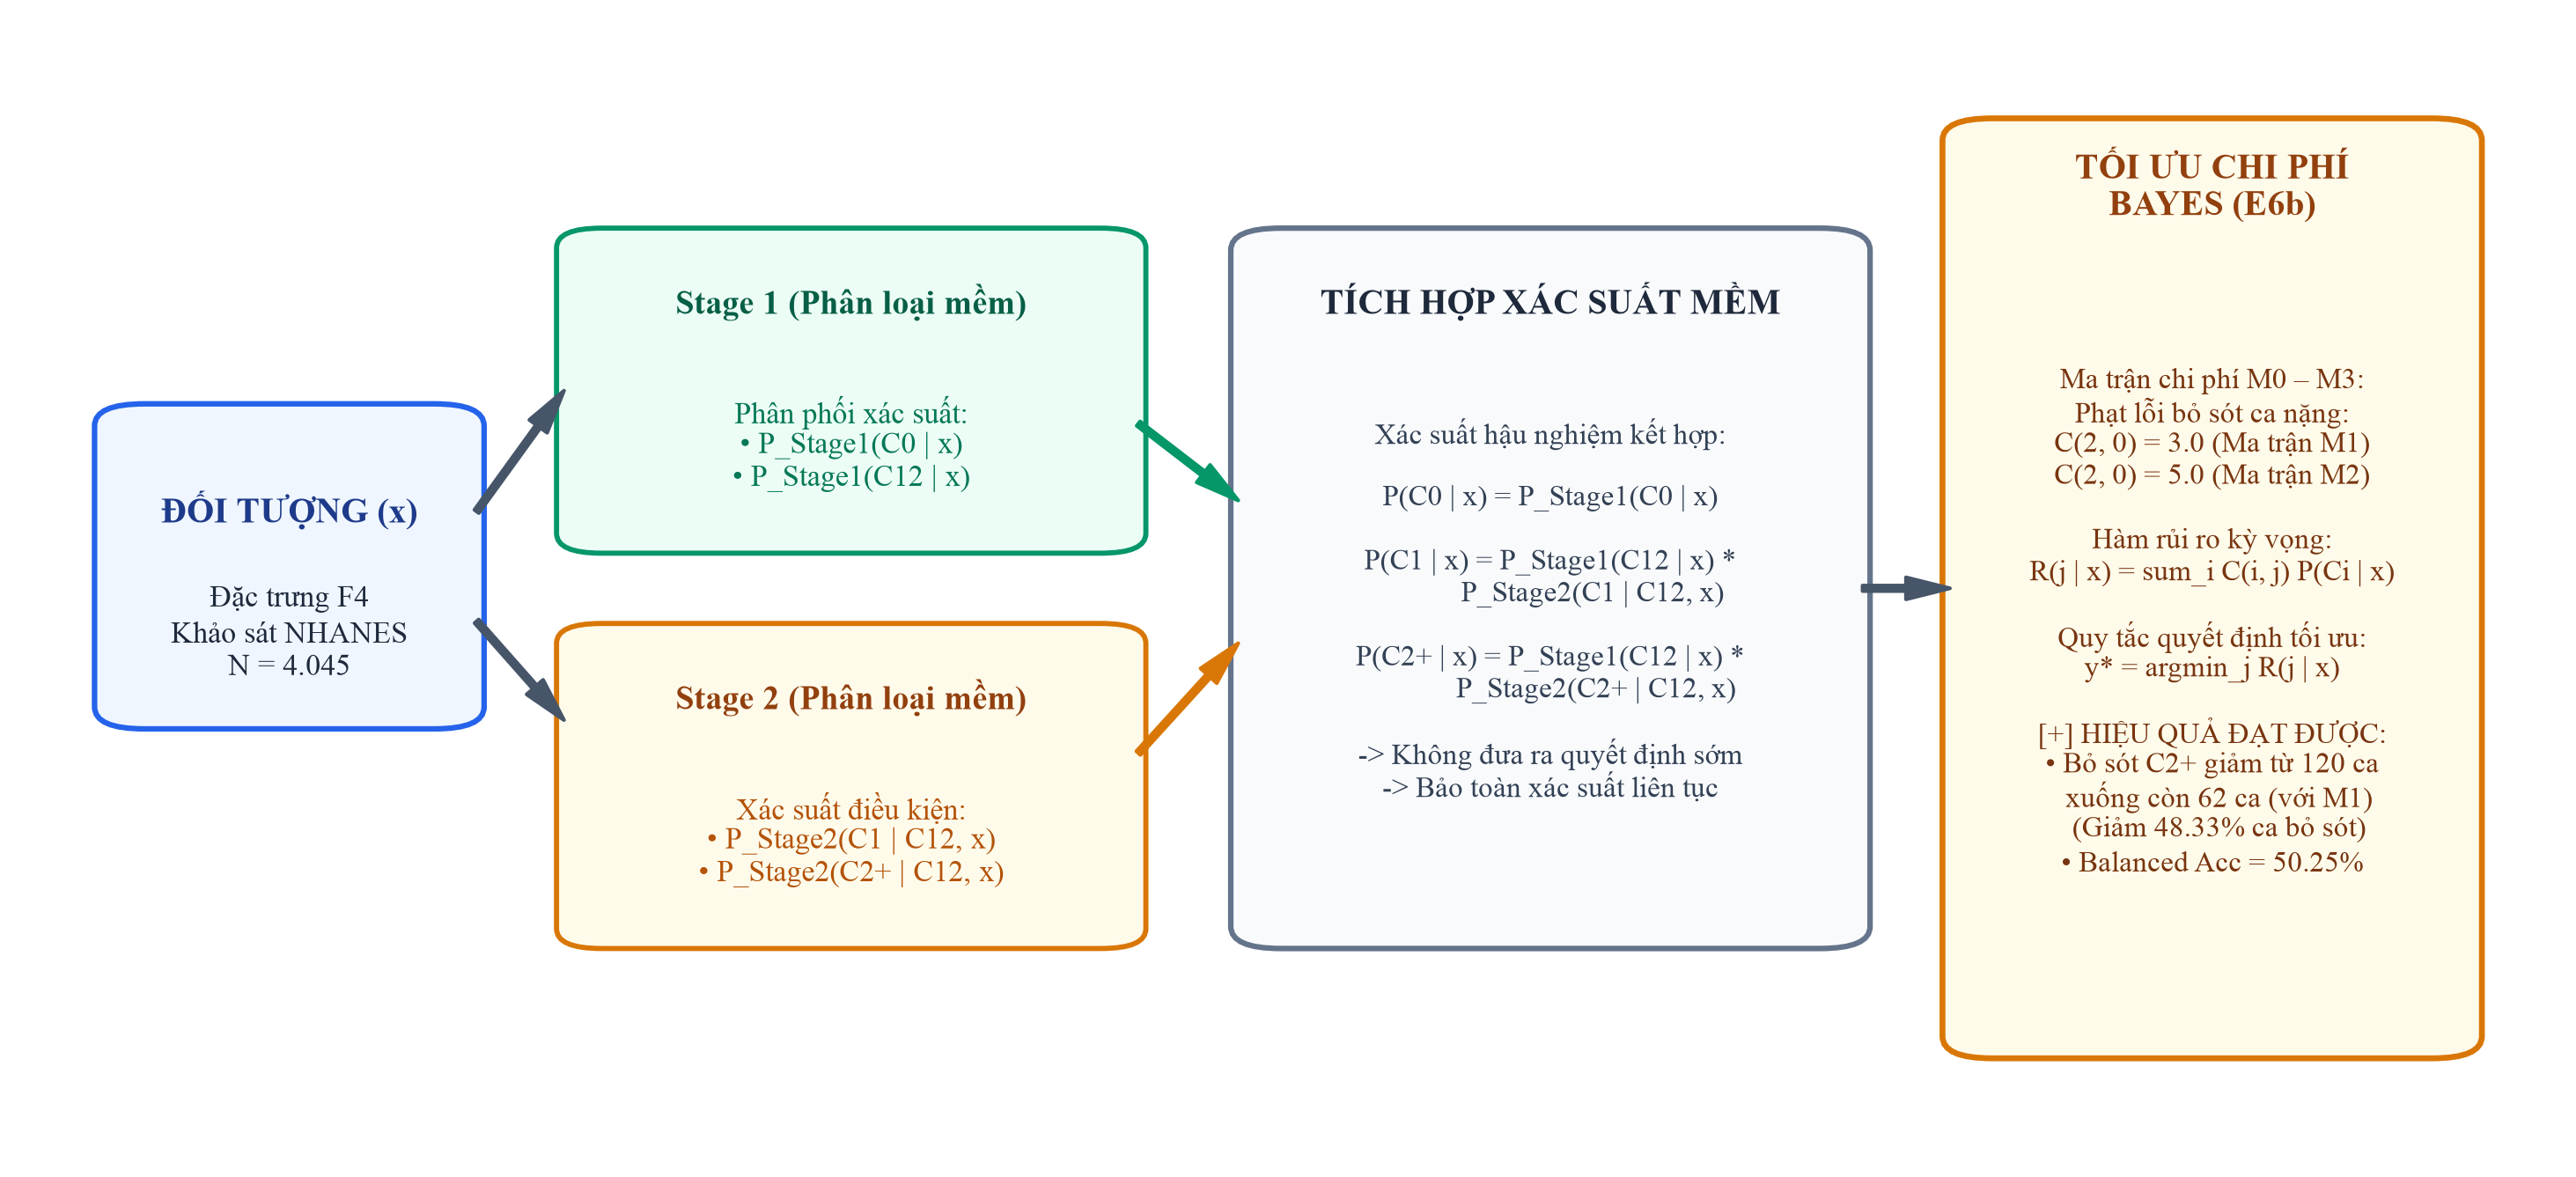
\includegraphics[width=\textwidth]{figures/fig3_5_soft_cost_sensitive.png}
\label{fig:soft-cost-architecture}
\end{figure}
\FloatBarrier

Phân phối xác suất hậu nghiệm kết hợp $\hat{\mathbf{p}} = [\hat{P}(C_0), \hat{P}(C_1), \hat{P}(C_2^+)]^T$ được tính theo công thức xác suất toàn phần:
\begin{align}
    \hat{P}(C_0 \mid \mathbf{x}) &= P_{\text{Stage 1}}(C_0 \mid \mathbf{x}) \\
    \hat{P}(C_1 \mid \mathbf{x}) &= P_{\text{Stage 1}}(C_{12} \mid \mathbf{x}) \cdot P_{\text{Stage 2}}(C_1 \mid C_{12}, \mathbf{x}) \\
    \hat{P}(C_2^+ \mid \mathbf{x}) &= P_{\text{Stage 1}}(C_{12} \mid \mathbf{x}) \cdot P_{\text{Stage 2}}(C_2^+ \mid C_{12}, \mathbf{x})
\end{align}

Từ phân phối xác suất hậu nghiệm mềm, hai cơ chế ra quyết định được áp dụng:
\begin{enumerate}
    \item \textbf{Cơ chế Argmax ($E_4, E_5$):} Chọn nhãn có xác suất lớn nhất $\hat{y} = \arg\max_k \hat{P}(C_k \mid \mathbf{x})$. Cấu hình $E_4$ sử dụng RF--RF; $E_5$ sử dụng RF--LR.
    \item \textbf{Cơ chế tối thiểu hóa rủi ro Bayes ($E_{6a}, E_{6b}$):} Đưa ma trận chi phí bất đối xứng $\mathbf{C} \in \mathbb{R}^{3 \times 3}$ vào hàm quyết định:
    \begin{equation}
        R(j \mid \mathbf{x}) = \sum_{i=0}^2 \hat{P}(C_i \mid \mathbf{x}) \cdot \mathbf{C}(i, j)
    \end{equation}
    \begin{equation}
        \hat{y}^* = \arg\min_{j \in \{0, 1, 2\}} R(j \mid \mathbf{x})
    \end{equation}
    trong đó $\mathbf{C}(i, j)$ là chi phí phạt khi nhãn thực tế là $C_i$ nhưng mô hình dự đoán là $C_j$. Nghiên cứu khảo sát 4 ma trận chi phí từ $M_0$ (chi phí đồng nhất) đến $M_3$ (phạt nặng nhất sai số bỏ sót ca nặng $\mathbf{C}(2, 0) = 8.0$). Ma trận được sử dụng chính trong báo cáo là $M_1$ ($\mathbf{C}(2, 0) = 3.0$). Chi tiết ma trận chi phí được trình bày tại Phụ lục \ref{app:cost-matrices}.
\end{enumerate}

\subsection{Mô hình phân loại thứ bậc ($E_7$)}
\label{subsec:e7-ordinal}

Do các mức độ triệu chứng PHQ-9 có tính chất thứ bậc ($C_0 < C_1 < C_2^+$), nhóm mô hình $E_7$ khai thác trực tiếp mối quan hệ trật tự này (Hình \ref{fig:ordinal-architecture}):

\begin{figure}[htbp]{Nguyên lý mô hình hóa thứ bậc: (a) Ordinal Logistic Regression và (b) Phân loại nhị phân tích lũy}
\centering
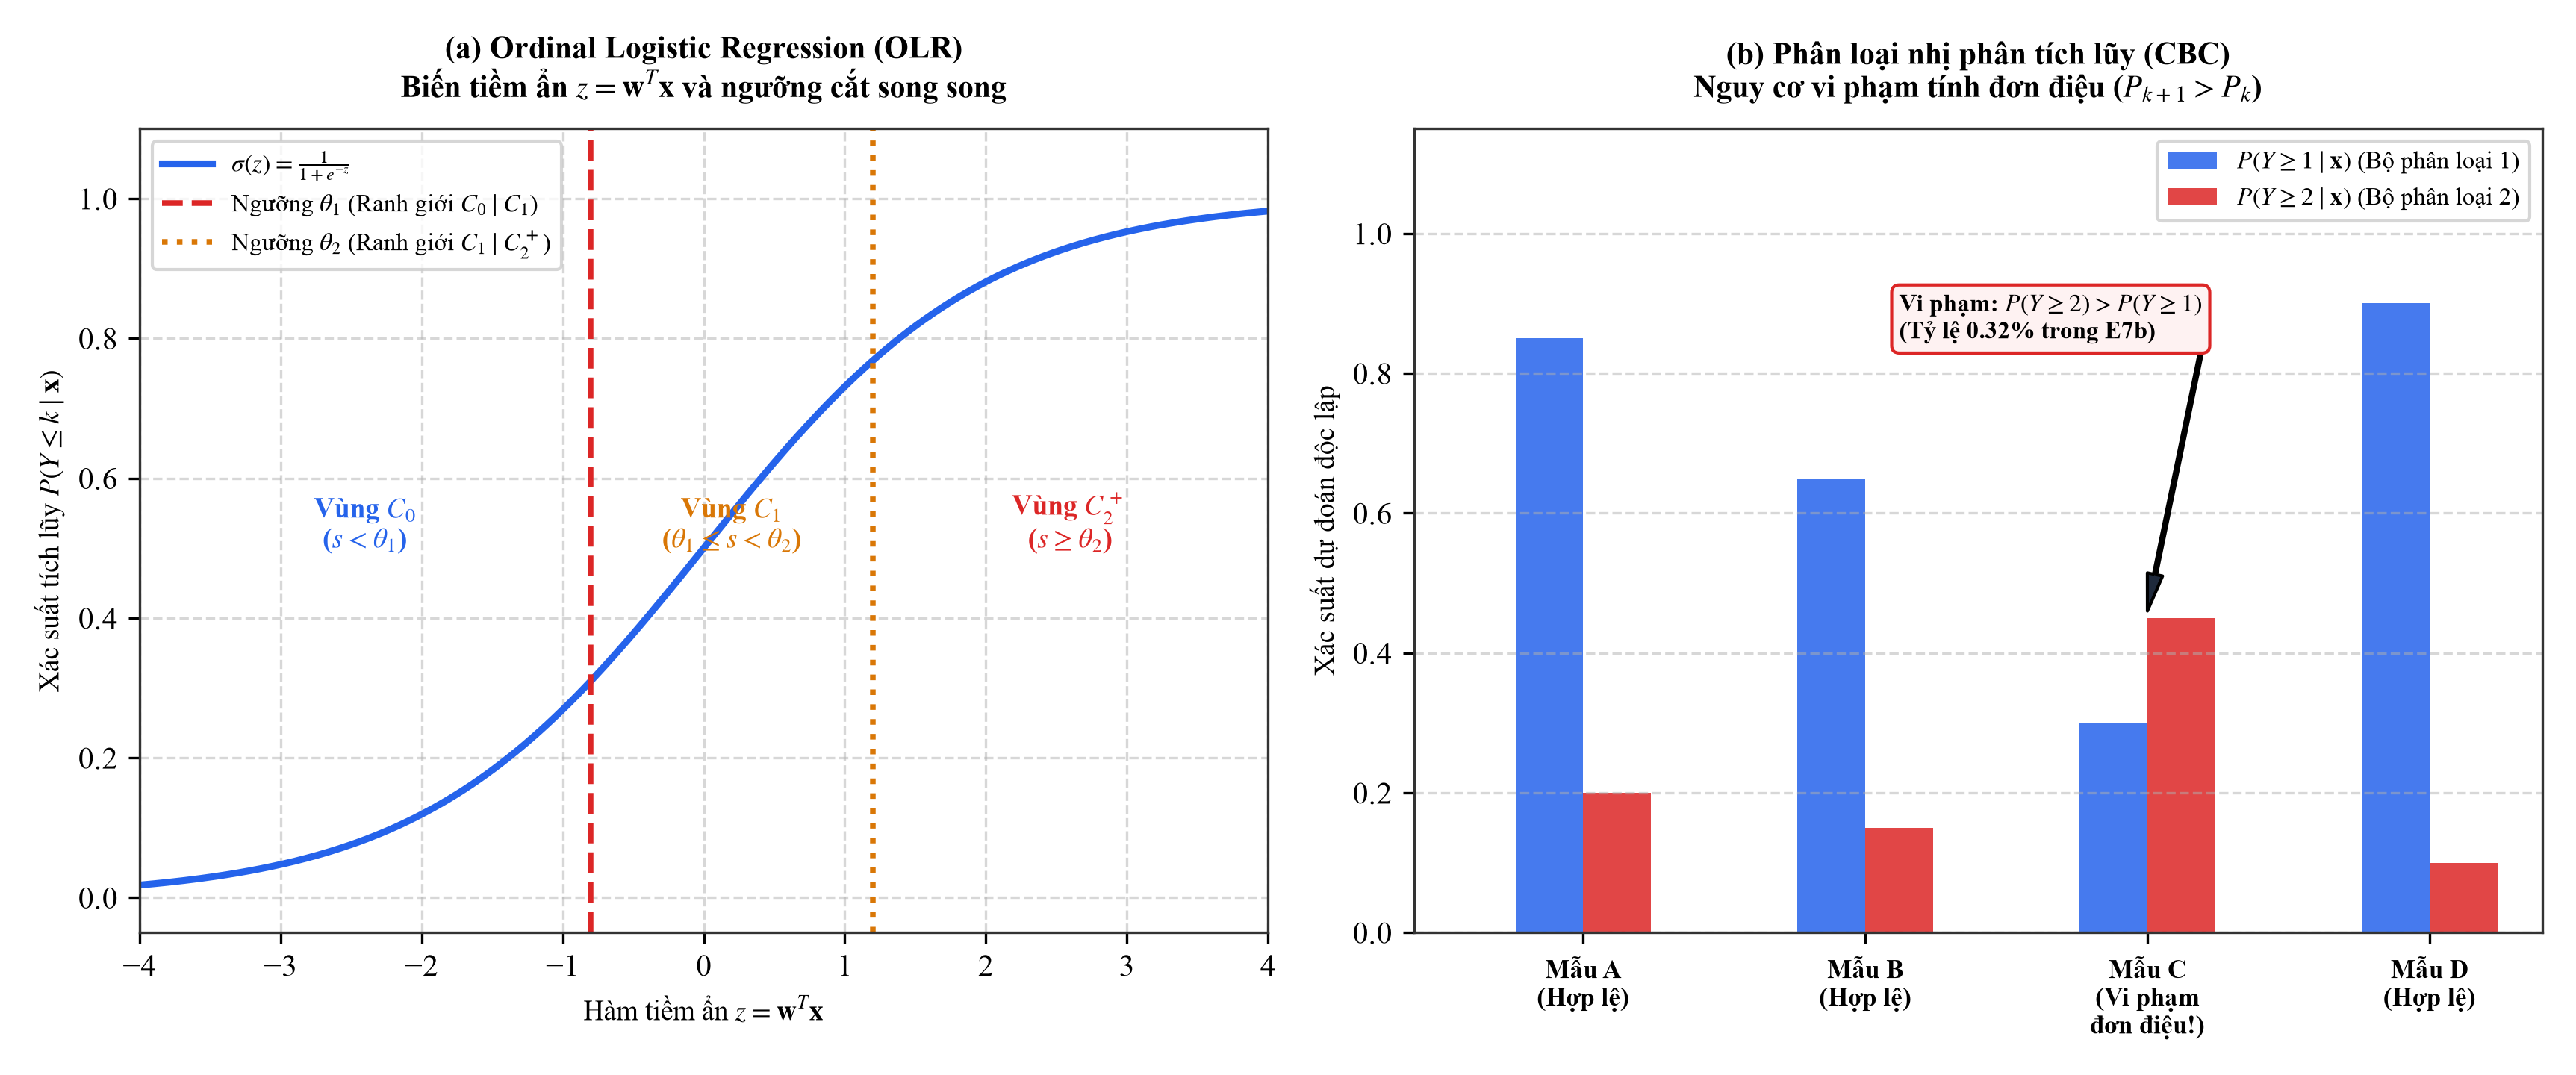
\includegraphics[width=\textwidth]{figures/fig3_6_ordinal_classification.png}
\label{fig:ordinal-architecture}
\end{figure}
\FloatBarrier

Nhóm thực nghiệm $E_7$ gồm hai hướng tiếp cận:
\begin{enumerate}
    \item \textbf{Ordinal Logistic Regression ($E_{7a}$ -- OLR):} 
    Mô hình giả định biến tiềm ẩn $z = \mathbf{w}^T \mathbf{x}$ cùng hai ngưỡng cắt $\theta_1 < \theta_2$. Xác suất tích lũy được mô hình hóa qua hàm phân phối Logistic:
    \begin{equation}
        P(Y \le k \mid \mathbf{x}) = \sigma(\theta_{k+1} - \mathbf{w}^T \mathbf{x}) = \frac{1}{1 + e^{-(\theta_{k+1} - \mathbf{w}^T \mathbf{x})}}
    \end{equation}
    Nghiên cứu khảo sát hai phiên bản: $E_{7a}$ Unweighted và $E_{7a}$ Balanced (gán trọng số nghịch đảo tần số lớp).
    \item \textbf{Phân loại nhị phân tích lũy ($E_{7b}$ -- Cumulative Binary Classification):} 
    Huấn luyện hai bộ phân loại nhị phân độc lập $h_1(\mathbf{x})$ cho bài toán $Y \ge 1$ và $h_2(\mathbf{x})$ cho bài toán $Y \ge 2$ bằng Random Forest. Xác suất từng lớp được suy luận bằng hiệu số tích lũy: $P(Y=0) = 1 - P(Y \ge 1)$, $P(Y=1) = P(Y \ge 1) - P(Y \ge 2)$, $P(Y=2) = P(Y \ge 2)$. Nếu xảy ra vi phạm đơn điệu $P(Y \ge 2) > P(Y \ge 1)$, giải thuật hiệu chỉnh ngưỡng cắt (isotonic clipping) được kích hoạt.
\end{enumerate}

\section{Thiết kế giao thức kiểm thử thực nghiệm}
\label{sec:giao-thuc-kiem-thu}

DepSev-ML áp dụng hai tầng giao thức kiểm định độc lập được minh họa trong Hình \ref{fig:evaluation-protocol}.

\begin{figure}[htbp]{Hai tầng giao thức kiểm thử: Nested 5-Fold Stratified CV và Temporal Validation}
\centering
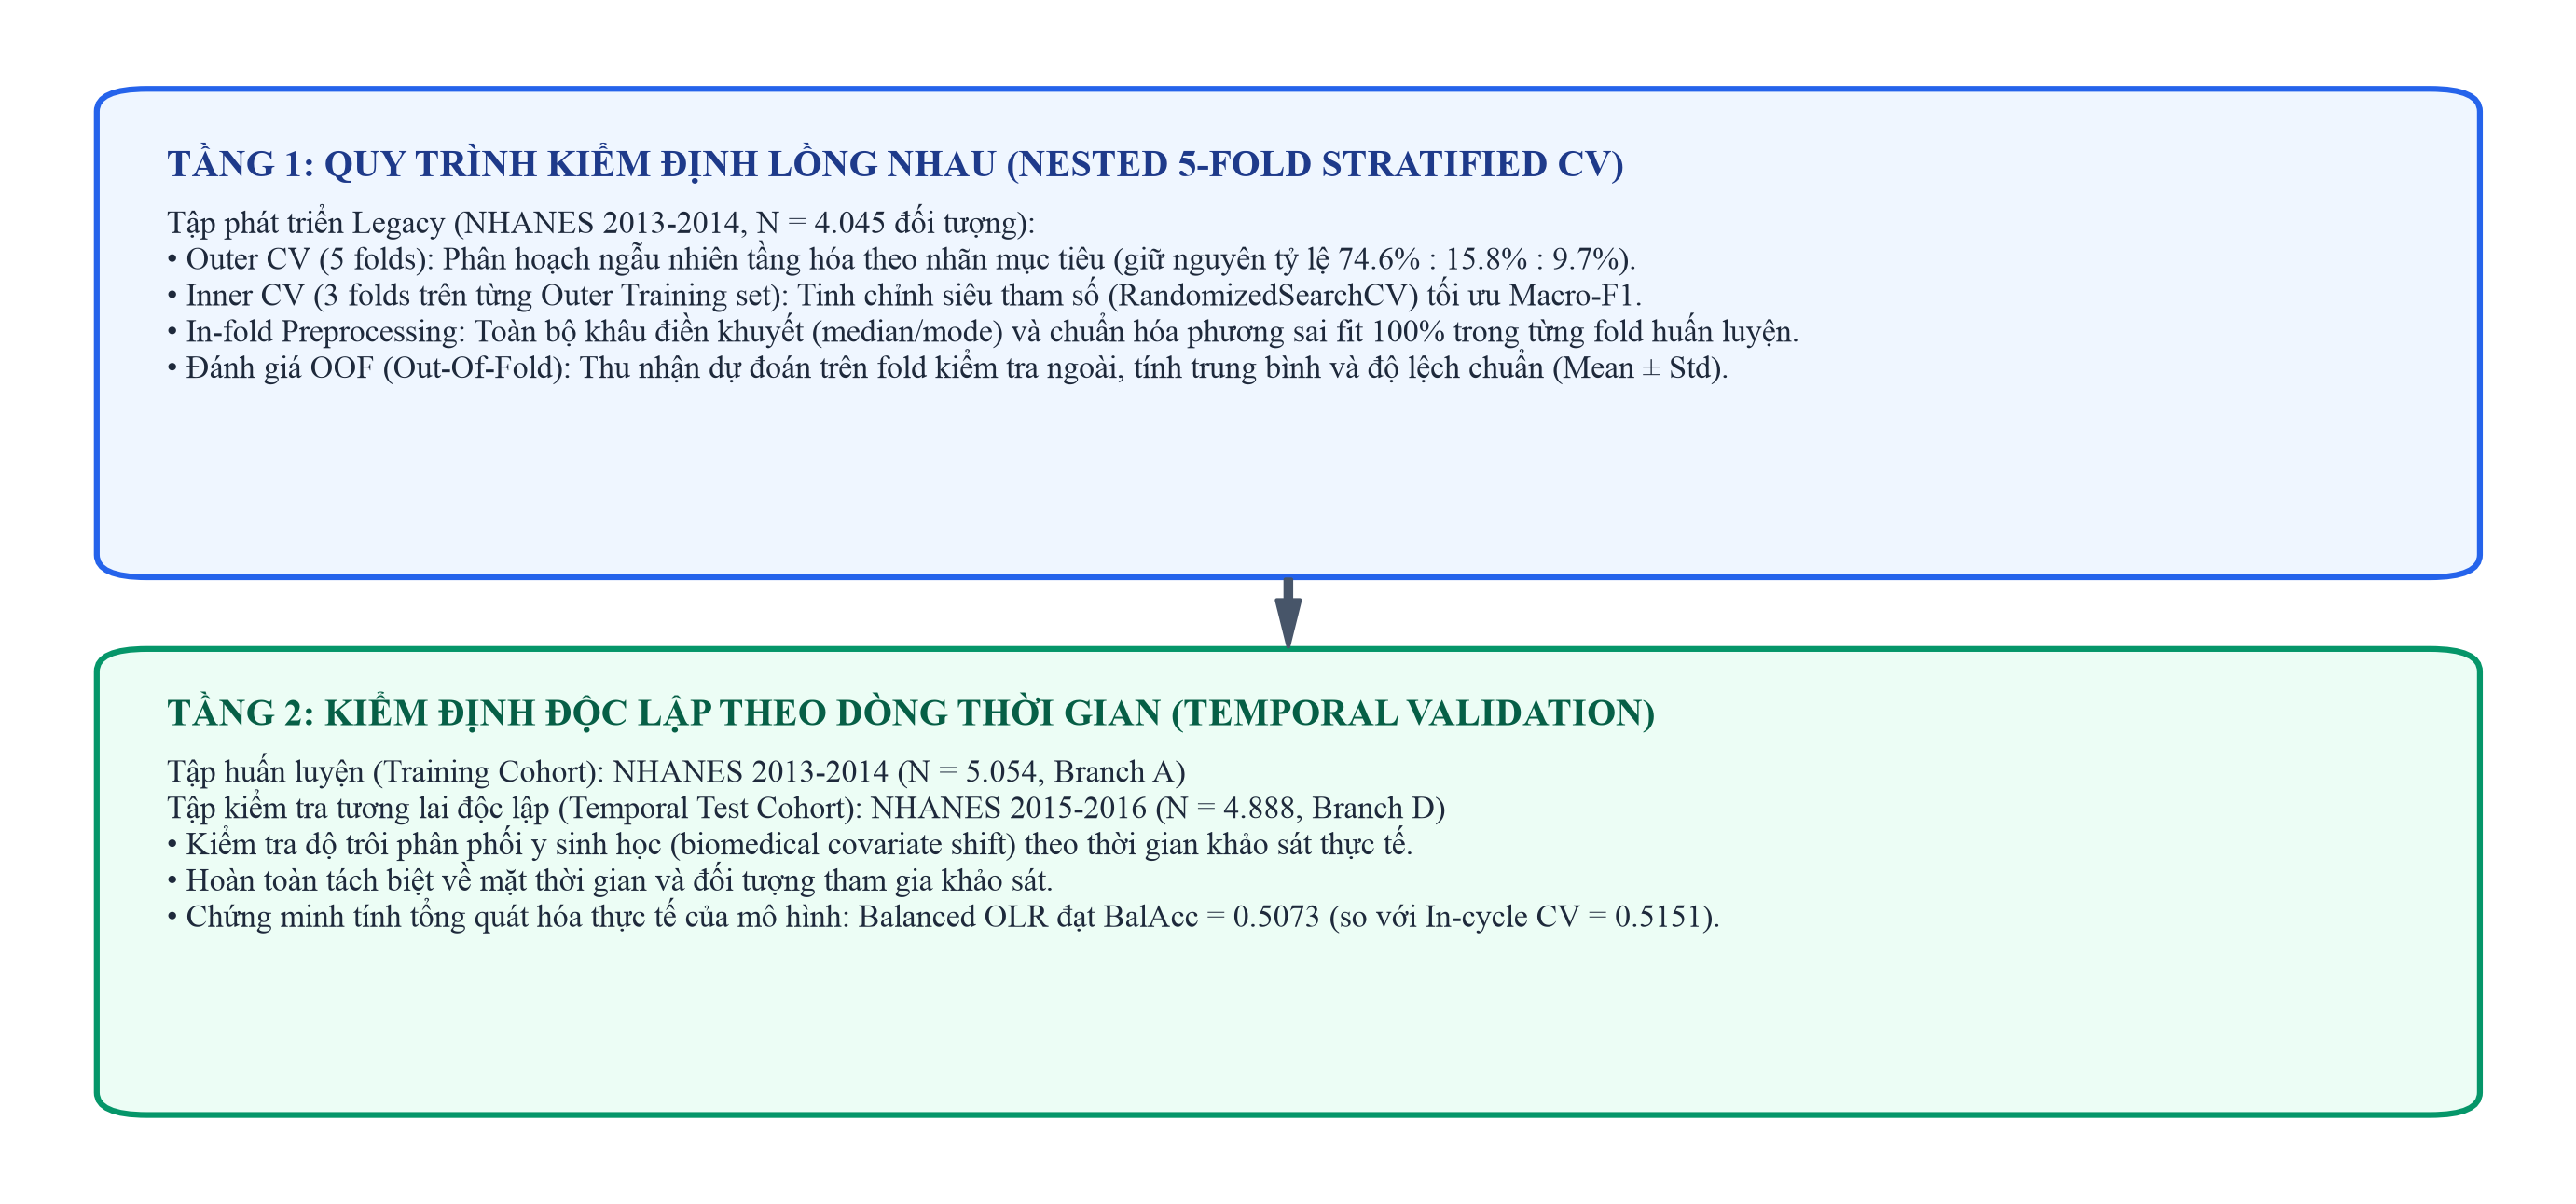
\includegraphics[width=\textwidth]{figures/fig3_7_evaluation_protocol.png}
\label{fig:evaluation-protocol}
\end{figure}
\FloatBarrier

\subsection{Quy trình kiểm định chéo lồng nhau (Nested 5-Fold Stratified CV)}
\label{subsec:nested-cv-protocol}

Trên tập dữ liệu phát triển Legacy ($N = 4.045$), quy trình kiểm định chéo lồng nhau được thực hiện:
\begin{itemize}
    \item \textbf{Outer CV (5 folds):} Phân chia dữ liệu thành 5 phần có bảo toàn tỷ lệ lớp (Stratified Split). Tại mỗi vòng lặp, 4 fold được dùng để huấn luyện và 1 fold dùng để đánh giá ngoài mẫu (Out-Of-Fold -- OOF).
    \item \textbf{Inner CV (3 folds trên từng Outer Training set):} Thực hiện RandomizedSearchCV với 12 cấu hình siêu tham số ngẫu nhiên trên độ đo Macro-F1 để tìm kiếm siêu tham số mà không sử dụng dữ liệu kiểm tra của Outer fold.
    \item Kết quả báo cáo là giá trị trung bình kèm độ lệch chuẩn ($\text{Mean} \pm \text{SD}$) trên 5 outer folds.
\end{itemize}

\subsection{Giao thức kiểm định ngoại suy theo dòng thời gian (Temporal Validation)}
\label{subsec:temporal-protocol}

Nhằm kiểm tra tính ổn định của mô hình trước hiện tượng dịch chuyển phân phối theo thời gian (covariate shift), nghiên cứu thiết lập giao thức kiểm định ngoại suy (Branch D): Tập huấn luyện gồm dữ liệu gộp hai chu kỳ NHANES 2011--2012 và 2013--2014 ($N = 9.693$); Tập kiểm tra độc lập gồm toàn bộ chu kỳ tiếp theo NHANES 2015--2016 ($N = 4.888$), áp dụng trên không gian 31 đặc trưng hài hòa hóa ($F_{4\_\text{common31}}$). Hai tập dữ liệu tách biệt về mặt thời gian khảo sát và không có đối tượng nào trùng lặp.

\section{Hệ thống độ đo đánh giá đa chiều}
\label{sec:he-thong-do-do}

Để đánh giá toàn diện các mô hình theo nhiều góc nhìn thực nghiệm khác nhau, nghiên cứu sử dụng hệ thống chỉ số đánh giá gồm:
\begin{enumerate}
    \item \textbf{Macro-F1:} Trung bình cộng F1-score của toàn bộ các lớp, phản ánh khả năng nhận diện cân bằng giữa các lớp mà không bị chi phối bởi lớp đa số.
    \item \textbf{Balanced Accuracy (BalAcc):} Trung bình cộng của Recall từng lớp $\text{BalAcc} = \frac{1}{K}\sum_k \text{Recall}_k$, đo lường độ nhạy trung bình của mô hình trên từng nhóm triệu chứng.
    \item \textbf{Class MAE (Sai số tuyệt đối theo lớp):} Đo khoảng cách bậc trung bình giữa mức độ dự đoán và mức độ thực tế: $\text{Class MAE} = \frac{1}{N} \sum_{i=1}^N |y_i - \hat{y}_i|$.
    \item \textbf{Quadratic Weighted Kappa (QWK):} Đo lường mức độ đồng thuận thứ bậc có tính đến mức phạt khoảng cách bậc hai \cite{cohen1968weighted}.
    \item \textbf{Đánh giá sự đánh đổi sai số sàng lọc:} Thống kê số lượng ca nặng bị phân loại nhầm thành bình thường ($C_2^+ \to C_0$) và số ca bình thường bị báo động nhầm thành nặng ($C_0 \to C_2^+$), phản ánh sự cân đối giữa an toàn phát hiện ca bệnh và chi phí theo dõi trong sàng lọc cộng đồng.
\end{enumerate}

\section{Tóm tắt chương}
\label{sec:tom-tat-chuong-3}

Chương 3 đã trình bày phương pháp luận của đề tài: từ quy trình tiền xử lý in-fold kiểm soát rò rỉ dữ liệu, 4 không gian đặc trưng lũy tiến ($F_1 \to F_4$), các thiết kế mô hình thực nghiệm ($E_0 \to E_7$), đến hai tầng giao thức kiểm định (Nested CV và Temporal Validation). Toàn bộ kết quả thực nghiệm thu được sẽ được phân tích chi tiết trong Chương \ref{ch:thuc-nghiem}.

\chapter{Thực nghiệm và thảo luận}
\label{ch:thuc-nghiem}

Chương này trình bày toàn bộ kết quả thực nghiệm và các phân tích nhằm trả lời 5 câu hỏi nghiên cứu (RQ1--RQ5) đã đặt ra. Các thực nghiệm được tổ chức theo hai hướng nghiên cứu chính:
(1) \textit{Hướng thứ nhất -- Khảo sát phân loại đa mức PHQ-9:} Đánh giá đóng góp của các nhóm đặc trưng ($F_1 \to F_4$), tinh chỉnh siêu tham số và đối chuẩn thuật toán, khảo sát biến thiên hiệu năng theo độ chi tiết nhãn ($T_2 \to T_5$), phân tích tương quan sinh lý và hình chiếu PCA, cùng thử nghiệm mở rộng dữ liệu đa chu kỳ NHANES ($N = 14.581$).
(2) \textit{Hướng thứ hai -- Khảo sát phân loại phân cấp và thứ bậc trên $T_3$:} Đánh giá có hệ thống 8 cấu hình mô hình thực nghiệm ($E_0 \to E_7$) trên không gian 3 nhóm ($C_0, C_1, C_2^+$); phân tích sự đánh đổi sai số theo ma trận chi phí Bayes; kiểm định ngoại suy theo dòng thời gian trên chu kỳ độc lập NHANES 2015--2016; và thảo luận tổng hợp 4 mô hình tiêu biểu đại diện cho các mục tiêu thực tế khác nhau.

\section{Thiết lập thực nghiệm và môi trường tính toán}
\label{sec:moi-truong-thuc-nghiem}

Môi trường thực nghiệm được thiết lập thống nhất:
\begin{itemize}
    \item \textbf{Phần cứng:} Máy trạm Apple Silicon (ARM64, M-series), bộ nhớ 16 GB RAM, ổ cứng SSD.
    \item \textbf{Môi trường phần mềm:} macOS Darwin Kernel 24.6.0; Python 3.13 chạy trong môi trường ảo hóa độc lập (.venv).
    \item \textbf{Thư viện tính toán:} scikit-learn 1.9.1 (các thuật toán học máy, tiền xử lý và kiểm định chéo); XGBoost 3.4.1; SciPy 1.18.1 (tối ưu hóa phi tuyến L-BFGS-B cho mô hình OLR); NumPy 2.5.3 và pandas 3.0.6; matplotlib 3.11.2 (trực quan hóa dữ liệu và xuất biểu đồ 300 DPI).
    \item \textbf{Kiểm soát ngẫu nhiên:} Hạt giống \textnormal{random\_state = 42} được cố định trên tất cả các phép chia fold, khởi tạo mô hình và lấy mẫu bootstrap nhằm bảo đảm tính tái lập kết quả.
\end{itemize}

\clearpage
\section{Đánh giá đóng góp của các nhóm đặc trưng (Feature Ablation)}
\label{sec:feature-ablation}

\subsection{Thiết lập thực nghiệm}
Thực nghiệm Feature Ablation nhằm trả lời câu hỏi nghiên cứu \textbf{RQ1}: Khảo sát mức độ đóng góp của bốn nhóm đặc trưng lũy tiến ($F_1 \to F_4$) đối với bài toán 5 mức độ $T_5$ ($C_0 \to C_4$). Thực nghiệm được thực hiện thông qua Stratified 5-Fold Cross-Validation trên tập phát triển Legacy ($N = 4.045$). Bốn thuật toán học máy cơ sở được đánh giá song song gồm: Logistic Regression (LR), Decision Tree (DT), Random Forest (RF) và XGBoost.

\subsection{Kết quả thực nghiệm}
Kết quả out-of-fold chi tiết được tổng hợp trong Bảng \ref{tab:ablation-results}. Hình \ref{fig:ablation-comparison} thể hiện xu hướng biến thiên của Macro-F1 trên các không gian đặc trưng.

\begin{table}[htbp]{Kết quả thực nghiệm Feature Ablation trên tập Legacy Development ($N = 4.045$, 5 lớp $T_5$)}
\centering
\footnotesize
\setlength{\tabcolsep}{3pt}
\label{tab:ablation-results}
\begin{tabularx}{\textwidth}{l c l >{\centering\arraybackslash}X >{\centering\arraybackslash}X >{\centering\arraybackslash}X}
\toprule
\textbf{Nhóm} & \textbf{$d$} & \textbf{Mô hình ML} & \textbf{Macro-F1 (Mean $\pm$ SD)} & \textbf{Balanced Acc (Mean $\pm$ SD)} & \textbf{Weighted-F1 (Mean $\pm$ SD)} \\
\midrule
\multirow{4}{*}{\textbf{$F_1$}} & \multirow{4}{*}{10} 
  & Logistic Regression & 0.1900 $\pm$ 0.0164 & 0.2420 $\pm$ 0.0299 & 0.4926 $\pm$ 0.0209 \\
& & Decision Tree        & 0.2081 $\pm$ 0.0121 & 0.2090 $\pm$ 0.0133 & 0.5926 $\pm$ 0.0081 \\
& & Random Forest       & 0.2052 $\pm$ 0.0072 & 0.2090 $\pm$ 0.0065 & 0.6314 $\pm$ 0.0107 \\
& & XGBoost             & 0.2173 $\pm$ 0.0147 & 0.2295 $\pm$ 0.0220 & 0.5577 $\pm$ 0.0072 \\
\midrule
\multirow{4}{*}{\textbf{$F_2$}} & \multirow{4}{*}{19} 
  & Logistic Regression & 0.2338 $\pm$ 0.0041 & 0.2942 $\pm$ 0.0299 & 0.5648 $\pm$ 0.0092 \\
& & Decision Tree        & 0.2319 $\pm$ 0.0154 & 0.2357 $\pm$ 0.0185 & 0.6144 $\pm$ 0.0093 \\
& & Random Forest       & 0.2350 $\pm$ 0.0180 & 0.2353 $\pm$ 0.0155 & 0.6557 $\pm$ 0.0097 \\
& & XGBoost             & 0.2447 $\pm$ 0.0143 & 0.2594 $\pm$ 0.0187 & 0.6002 $\pm$ 0.0123 \\
\midrule
\multirow{4}{*}{\textbf{$F_3$}} & \multirow{4}{*}{29} 
  & Logistic Regression & 0.2390 $\pm$ 0.0084 & 0.3194 $\pm$ 0.0284 & 0.5637 $\pm$ 0.0071 \\
& & Decision Tree        & 0.2388 $\pm$ 0.0127 & 0.2408 $\pm$ 0.0148 & 0.6195 $\pm$ 0.0100 \\
& & Random Forest       & 0.2299 $\pm$ 0.0045 & 0.2314 $\pm$ 0.0047 & 0.6671 $\pm$ 0.0085 \\
& & XGBoost             & 0.2588 $\pm$ 0.0402 & 0.2713 $\pm$ 0.0490 & 0.6224 $\pm$ 0.0154 \\
\midrule
\multirow{4}{*}{\textbf{$F_4$}} & \multirow{4}{*}{34} 
  & Logistic Regression & 0.2399 $\pm$ 0.0148 & \textbf{0.3216 $\pm$ 0.0508} & 0.5591 $\pm$ 0.0112 \\
& & Decision Tree        & 0.2412 $\pm$ 0.0175 & 0.2450 $\pm$ 0.0206 & 0.6181 $\pm$ 0.0098 \\
& & Random Forest       & 0.2232 $\pm$ 0.0099 & 0.2253 $\pm$ 0.0075 & \textbf{0.6625 $\pm$ 0.0091} \\
& & XGBoost             & \textbf{0.2707 $\pm$ 0.0428} & 0.2837 $\pm$ 0.0485 & 0.6344 $\pm$ 0.0148 \\
\bottomrule
\end{tabularx}
\end{table}


\begin{figure}[htbp]{So sánh hiệu năng Macro-F1 của 4 thuật toán trên các nhóm đặc trưng lũy tiến $F_1 \to F_4$}
\centering
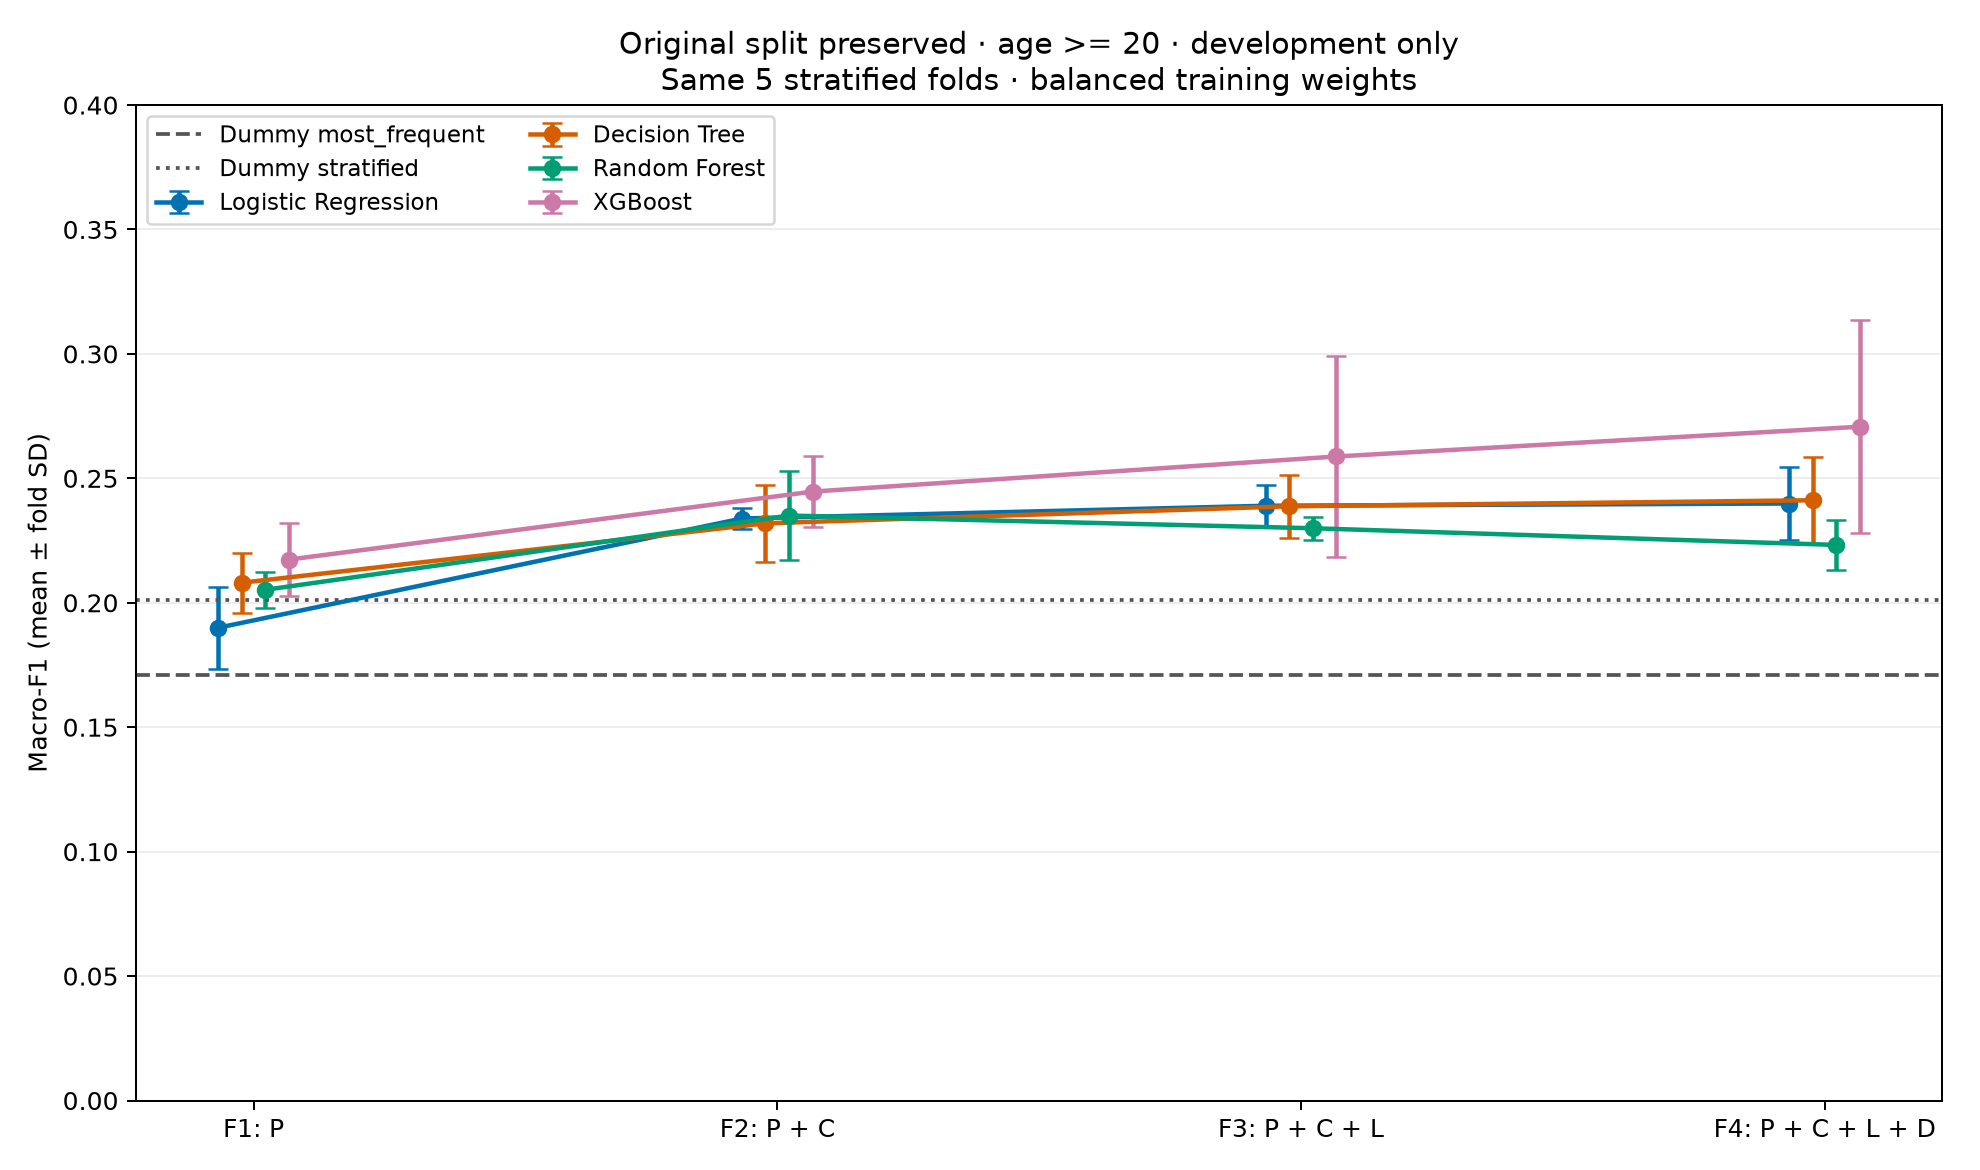
\includegraphics[width=0.9\textwidth]{figures/feature_group_comparison_final_protocol.png}
\label{fig:ablation-comparison}
\end{figure}
\FloatBarrier

\subsection{Phân tích kết quả}
Từ kết quả Bảng \ref{tab:ablation-results}, một số phát hiện được ghi nhận:
\begin{enumerate}
    \item \textbf{Đóng góp của nhóm Tiền sử bệnh lý ($F_1 \to F_2$):} Nhóm $F_1$ (10 biến gồm thể chất, huyết áp và 5 xét nghiệm máu) chỉ mang lại Macro-F1 khiêm tốn trên mọi thuật toán (0.1900 với LR, 0.2052 với RF và 0.2173 với XGBoost). Khi bổ sung 9 biến tiền sử bệnh mạn tính ở nhóm $F_2$, hiệu năng tăng rõ rệt trên tất cả các mô hình: LR tăng từ 0.1900 lên 0.2338 (+23.1\%), RF tăng từ 0.2052 lên 0.2350 (+14.5\%), và XGBoost tăng từ 0.2173 lên 0.2447 (+12.6\%). Điều này cho thấy tiền sử bệnh mạn tính cung cấp thông tin hữu ích cho việc phân tầng nguy cơ.
    \item \textbf{Đóng góp của nhóm Lối sống và Nhân khẩu học ($F_3, F_4$):} Nhóm thói quen sinh hoạt (giấc ngủ, vận động thể lực, hút thuốc, rượu bia) và nhân khẩu học (tuổi, giới tính, học vấn, tỷ lệ thu nhập) tiếp tục nâng hiệu năng của XGBoost lên mức Macro-F1 cao nhất là \textbf{0.2707 $\pm$ 0.0428} (Balanced Accuracy = 0.2837 $\pm$ 0.0485), tương đương mức tăng +24.6\% so với khi chỉ sử dụng $F_1$ (0.2173). Với Random Forest, Macro-F1 cũng tăng từ 0.2052 ($F_1$) lên 0.2232 ($F_4$); với Logistic Regression tăng từ 0.1900 lên 0.2152.
    \item \textbf{Sự khác biệt giữa Weighted-F1 và Macro-F1:} Weighted-F1 luôn đạt mức cao (0.49 -- 0.67) do bị chi phối bởi lớp đa số $C_0$ (chiếm ~75\%). Ngược lại, Macro-F1 dao động quanh mức 0.19 -- 0.27, phản ánh đúng mức độ khó khăn khi nhận diện các lớp có triệu chứng.
\end{enumerate}

\section{Tinh chỉnh siêu tham số và khảo sát mô hình kết hợp}
\label{sec:tuning-va-ensemble}

\subsection{Tinh chỉnh Nested Cross-Validation và Đối chuẩn thuật toán}
Để lựa chọn cấu hình mô hình cơ sở một cách khách quan và hạn chế thiên lệch lạc quan, nghiên cứu áp dụng quy trình kiểm định chéo lồng nhau (Nested CV): Outer 5 folds đánh giá khả năng khái quát hóa, Inner 3 folds thực hiện RandomizedSearchCV với 12 cấu hình siêu tham số trên độ đo Macro-F1.

Kết quả đối chuẩn giữa các thuật toán học máy cơ sở qua Outer Nested CV được tổng hợp trong Bảng \ref{tab:nested-cv-comparison}.

\begin{table}{Kết quả đánh giá đối chuẩn các thuật toán học máy cơ sở qua Nested Cross-Validation (5 lớp $T_5$)}
\centering
\footnotesize
\setlength{\tabcolsep}{3.5pt}
\label{tab:nested-cv-comparison}
\begin{tabularx}{\textwidth}{p{3.2cm} c >{\centering\arraybackslash}X >{\centering\arraybackslash}X >{\centering\arraybackslash}X c}
\toprule
\textbf{Thuật toán ML} & \textbf{Đặc trưng} & \textbf{Macro-F1 (Mean $\pm$ SD)} & \textbf{Balanced Acc (Mean $\pm$ SD)} & \textbf{Weighted-F1 (Mean $\pm$ SD)} & \textbf{$\Delta$ so với Baseline} \\
\midrule
Logistic Regression & $F_4$ (34) & 0.2407 $\pm$ 0.0173 & \textbf{0.3253 $\pm$ 0.0532} & 0.5599 $\pm$ 0.0128 & $+0.0009$ \\
Decision Tree (Gini) & $F_4$ (34) & 0.2412 $\pm$ 0.0175 & 0.2450 $\pm$ 0.0206 & 0.6181 $\pm$ 0.0098 & $0.0000$ \\
XGBoost (Tuned) & $F_3$ (29) & 0.2516 $\pm$ 0.0267 & 0.2658 $\pm$ 0.0355 & 0.6130 $\pm$ 0.0152 & $-0.0071$ \\
XGBoost (Tuned) & $F_4$ (34) & 0.2621 $\pm$ 0.0353 & 0.2743 $\pm$ 0.0373 & 0.6196 $\pm$ 0.0195 & $-0.0087$ \\
\textbf{Random Forest (Tuned)} & $F_4$ (34) & \textbf{0.2755 $\pm$ 0.0270} & 0.2983 $\pm$ 0.0325 & \textbf{0.6437 $\pm$ 0.0087} & \textbf{+0.0523} \\
\bottomrule
\end{tabularx}

\vspace{0.12cm}
\raggedright
\scriptsize
\textit{Ghi chú:} Kết quả báo cáo là trung bình $\pm$ độ lệch chuẩn trên 5 outer folds của Nested Cross-Validation. Cấu hình Random Forest (Tuned) được tối ưu hóa siêu tham số in-fold; bộ siêu tham số xuất hiện lặp lại phổ biến nhất sau đó được cố định ("Frozen RF Spec": \textnormal{n\_estimators = 150, max\_depth = 8, max\_features = 0.5, min\_samples\_split = 10, min\_samples\_leaf = 8}) làm mốc đối chuẩn cho các thử nghiệm tiếp theo.
\end{table}



\textbf{Phân tích kết quả và lý do lựa chọn Random Forest làm mô hình cơ sở chính:}
Từ Bảng \ref{tab:nested-cv-comparison}, Random Forest đạt chỉ số Macro-F1 trung bình cao nhất trong nhóm các mô hình phẳng được khảo sát là \textbf{0.2755 $\pm$ 0.0270} và Weighted-F1 đạt \textbf{0.6437 $\pm$ 0.0087}, cải thiện \textbf{+0.0523} so với cấu hình mặc định chưa tinh chỉnh ($0.2232$).

Lý do lựa chọn Random Forest được xác định dựa trên kết quả thực nghiệm:
\begin{enumerate}
    \item \textit{Đánh giá khách quan trên các chỉ số:} Logistic Regression đạt Balanced Accuracy cao hơn ($0.3253 \pm 0.0532$) nhờ mặt phẳng phân tách tuyến tính trơn mượt phân bổ dự đoán sang các lớp nhỏ, nhưng Macro-F1 lại thấp hơn ($0.2407$). XGBoost đạt Macro-F1 là $0.2621 \pm 0.0353$ nhưng có độ lệch chuẩn lớn hơn giữa các fold so với Random Forest.
    \item \textit{Tính ổn định phương sai:} Random Forest thể hiện khả năng giảm phương sai tốt nhờ kết hợp Bootstrap Sampling và ngẫu nhiên hóa đặc trưng, giúp hạn chế ảnh hưởng của nhiễu đo lường trên dữ liệu y tế dạng bảng NHANES. Mô hình đạt được sự cân bằng tương đối tốt giữa việc nhận diện các lớp nhỏ và độ chính xác tổng thể.
\end{enumerate}

Do đó, cấu hình Random Forest tối ưu (\textnormal{n\_estimators = 150, max\_depth = 8, max\_features = 0.5, min\_samples\_split = 10, min\_samples\_leaf = 8, class\_weight = 'balanced\_subsample'}) được cố định thành \textbf{Frozen Random Forest Spec} (chi tiết tại Phụ lục \ref{app:hyperparameters}) làm mô hình cơ sở chính cho các phân tích tiếp theo.

\subsection{Khảo sát mô hình học kết hợp (Ensemble Study)}
Nghiên cứu kiểm tra xem liệu các phương pháp kết hợp mô hình (Soft Voting và Stacking) có mang lại cải thiện đáng kể so với Random Forest đơn lẻ hay không (Hình \ref{fig:ensemble-comparison}):
\begin{itemize}
    \item \textbf{Frozen Random Forest (Đơn lẻ)}: Macro-F1 = \textbf{0.2741 $\pm$ 0.0252}, Balanced Accuracy = \textbf{0.3015 $\pm$ 0.0294}.
    \item \textbf{Soft Voting (RF + XGBoost)}: Macro-F1 = 0.2748 $\pm$ 0.0248 (tăng nhẹ +0.0007).
    \item \textbf{Stacking Classifier (Meta-LR)}: Macro-F1 = 0.2585 $\pm$ 0.0226 (giảm -0.0156).
\end{itemize}

\begin{figure}[htbp]{So sánh hiệu năng giữa mô hình đơn nhất Frozen Random Forest và các mô hình kết hợp Ensemble}
\centering
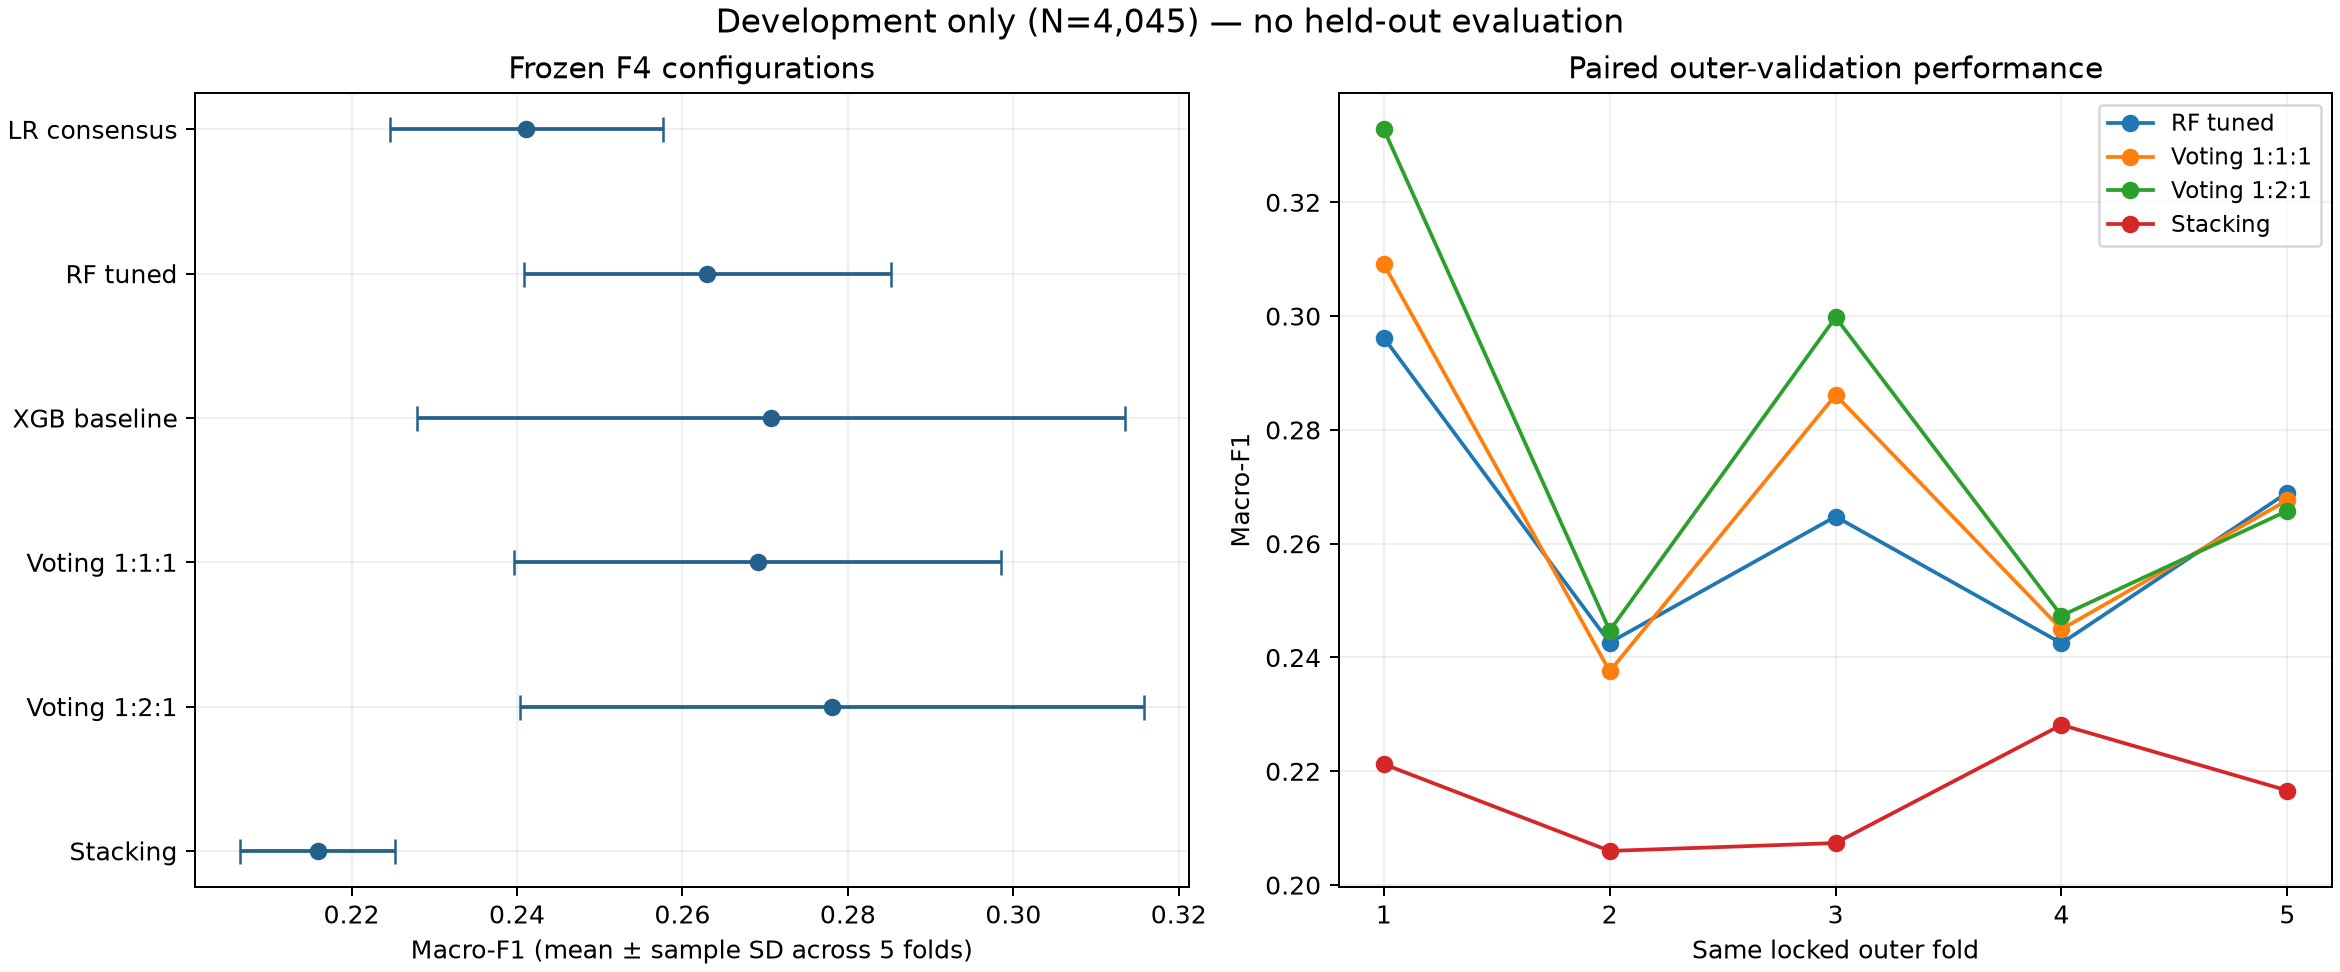
\includegraphics[width=0.85\textwidth]{figures/ensemble_comparison.png}
\label{fig:ensemble-comparison}
\end{figure}
\FloatBarrier

Theo tiêu chí thực nghiệm, một mô hình phức tạp hơn chỉ được ưu tiên nếu cải thiện Macro-F1 tối thiểu +0.01 một cách ổn định qua các folds. Cả Soft Voting và Stacking đều không đáp ứng tiêu chí này. Do đó, nghiên cứu giữ nguyên Frozen Random Forest làm mô hình cơ sở.

\section{Khảo sát độ chi tiết nhãn mục tiêu ($T_2 \to T_5$)}
\label{sec:target-granularity}

\subsection{Khảo sát biến thiên hiệu năng theo độ chi tiết nhãn}
Để trả lời câu hỏi nghiên cứu \textbf{RQ2}, nghiên cứu khảo sát sự thay đổi hiệu năng khi chuyển từ bài toán nhị phân ($T_2$) sang các mức độ chi tiết hơn ($T_3, T_4, T_5$) trên cùng mô hình Frozen Random Forest và không gian đặc trưng $F_4$ ($N = 4.045$).

Kết quả out-of-fold được trình bày trong Bảng \ref{tab:granularity-results}. Sự biến thiên được minh họa trong Hình \ref{fig:granularity-curves} và Hình \ref{fig:granularity-dist}.

\begin{table}{Hiệu năng mô hình Random Forest theo độ chi tiết nhãn mục tiêu ($T_2 \to T_5$) trên Legacy Development ($N = 4.045$)}
\centering
\footnotesize
\setlength{\tabcolsep}{3pt}
\label{tab:granularity-results}
\begin{tabularx}{\textwidth}{l c >{\centering\arraybackslash}X >{\centering\arraybackslash}X >{\centering\arraybackslash}X >{\centering\arraybackslash}X}
\toprule
\textbf{Nhiệm vụ} & \textbf{Số lớp} & \textbf{Độ chính xác (Acc)} & \textbf{Macro-F1 (Mean $\pm$ SD)} & \textbf{Balanced Acc} & \textbf{Weighted-F1} \\
\midrule
$T_2$ (Không vs Có) & 2 & 74.24\% $\pm$ 1.26\% & \textbf{0.6639 $\pm$ 0.0113} & \textbf{0.6659 $\pm$ 0.0122} & 0.7436 $\pm$ 0.0100 \\
$T_3$ ($C_0, C_1, C_2^+$) & 3 & 64.10\% $\pm$ 2.79\% & 0.4354 $\pm$ 0.0075 & 0.4667 $\pm$ 0.0101 & 0.6538 $\pm$ 0.0156 \\
$T_4$ ($C_0, C_1, C_2, C_{3+4}$) & 4 & 61.06\% $\pm$ 2.58\% & 0.3380 $\pm$ 0.0177 & 0.3661 $\pm$ 0.0202 & 0.6351 $\pm$ 0.0169 \\
$T_5$ (5 mức chuẩn PHQ-9) & 5 & 61.38\% $\pm$ 2.03\% & 0.2630 $\pm$ 0.0222 & 0.2805 $\pm$ 0.0199 & 0.6339 $\pm$ 0.0116 \\
\bottomrule
\end{tabularx}
\end{table}


\begin{figure}[htbp]{Biến thiên hiệu năng Macro-F1 và Balanced Accuracy từ bài toán nhị phân $T_2$ đến đa lớp $T_5$}
\centering
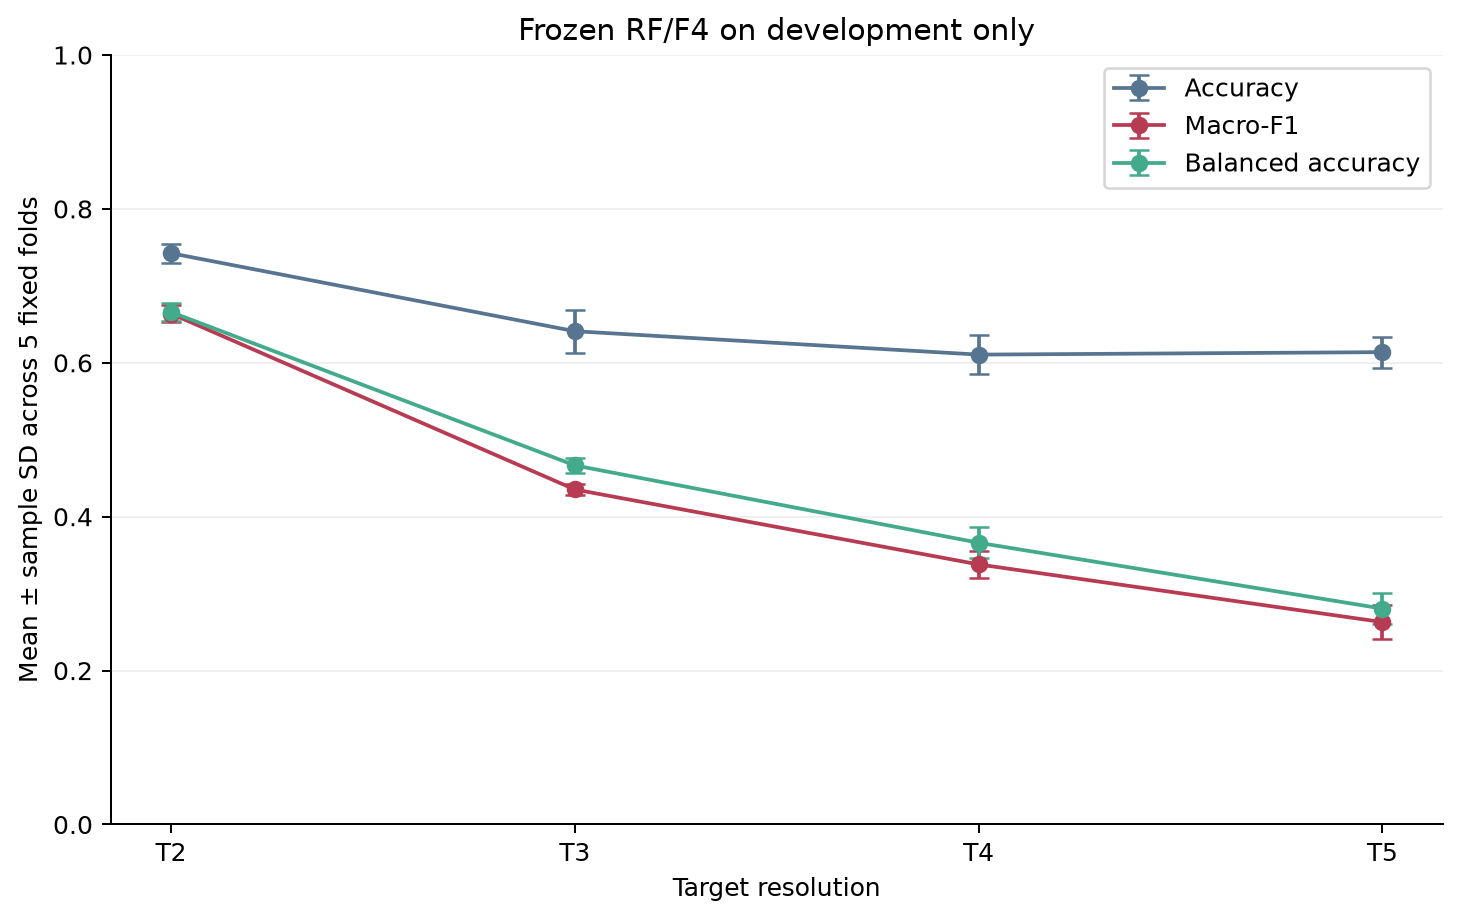
\includegraphics[width=0.85\textwidth]{figures/granularity_performance.png}
\label{fig:granularity-curves}
\end{figure}
\FloatBarrier

\begin{figure}[htbp]{Biến động cấu trúc phân bố các lớp khi tăng độ phân giải nhãn mục tiêu từ $T_2$ đến $T_5$}
\centering
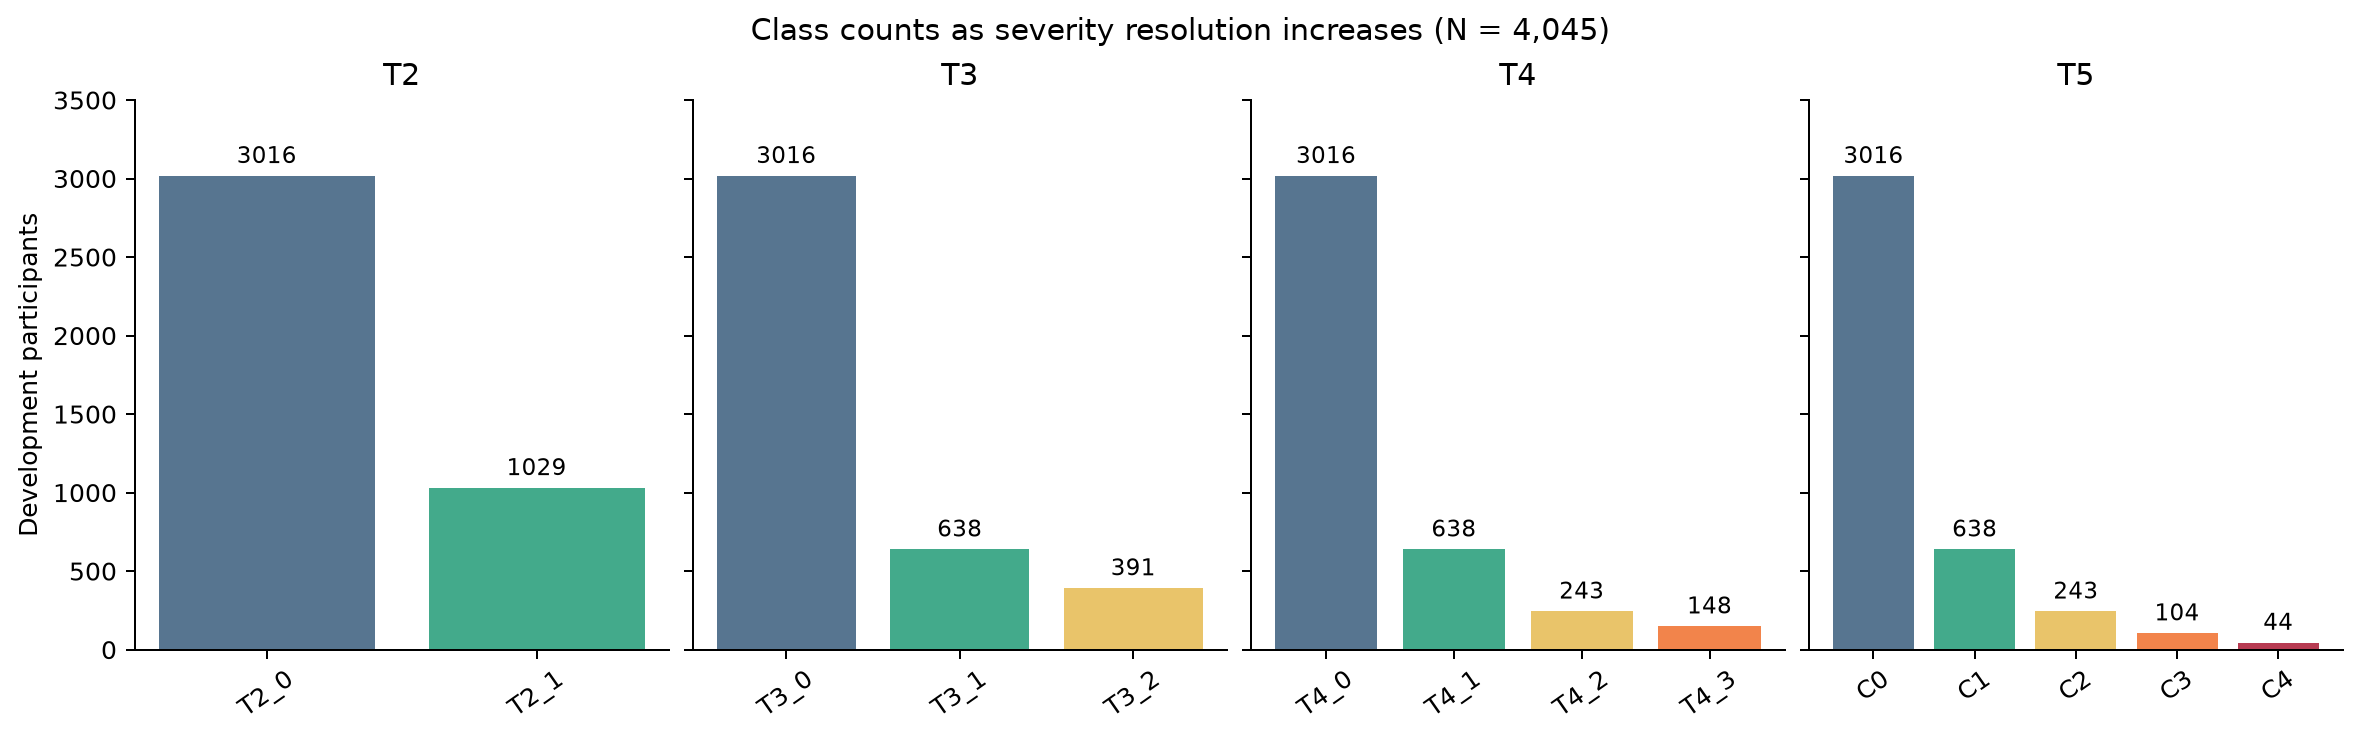
\includegraphics[width=0.85\textwidth]{figures/granularity_class_distribution.png}
\label{fig:granularity-dist}
\end{figure}
\FloatBarrier

\subsection{Phân tích biến thiên ranh giới và Ma trận nhầm lẫn $T_5$}
Từ Bảng \ref{tab:granularity-results}, mức độ thay đổi hiệu năng đáng chú ý nhất diễn ra tại bước chuyển từ $T_2$ sang $T_3$: Macro-F1 thay đổi từ \textbf{0.6639 sang 0.4354} (-34.4\%), và Balanced Accuracy từ \textbf{0.6659 sang 0.4667} (-29.9\%). Khi tiếp tục tăng độ chi tiết lên $T_4$ và $T_5$, Macro-F1 đạt lần lượt 0.3380 và 0.2630. Cần lưu ý rằng $T_2$ và $T_3$ có không gian nhãn mục tiêu khác nhau (2 lớp so với 3 lớp); do đó sự biến thiên này phản ánh độ phức tạp gia tăng khi mô hình phải phân định ranh giới giữa các nhóm triệu chứng liền kề.

Để phân tích chi tiết kết quả dự đoán của mô hình Random Forest trên 5 lớp phẳng $T_5$, ma trận nhầm lẫn $5 \times 5$ được trích xuất từ dữ liệu thực nghiệm out-of-fold ($N = 4.045$, nguồn từ \textnormal{granularity\_confusion\_matrices.csv}) và được thể hiện trong Hình \ref{fig:t5-confusion-matrix}:
\begin{itemize}
    \item \textbf{Lớp tối thiểu $C_0$ (3.016 mẫu):} 2.295 mẫu dự đoán đúng (Recall = 76.09\%), 385 mẫu nhầm sang $C_1$, 272 mẫu sang $C_2$, 55 mẫu sang $C_3$, 9 mẫu sang $C_4$.
    \item \textbf{Lớp nhẹ $C_1$ (638 mẫu):} Chỉ 101 mẫu dự đoán đúng (\textbf{Recall = 15.83\%}), trong khi có tới \textbf{344 mẫu (53.92\%) bị xếp sang $C_0$}. 149 mẫu nhầm sang $C_2$, 38 mẫu sang $C_3$, 6 mẫu sang $C_4$.
    \item \textbf{Lớp vừa $C_2$ (243 mẫu):} 67 mẫu đúng (Recall = 27.57\%), 73 mẫu nhầm sang $C_0$, 65 mẫu sang $C_1$, 30 mẫu sang $C_3$, 8 mẫu sang $C_4$.
    \item \textbf{Lớp nặng vừa $C_3$ (104 mẫu):} 19 mẫu đúng (Recall = 18.27\%), 24 mẫu nhầm sang $C_0$, 19 mẫu sang $C_1$, 40 mẫu sang $C_2$, 2 mẫu sang $C_4$.
    \item \textbf{Lớp nặng $C_4$ (44 mẫu):} \textbf{Chỉ 1 mẫu được dự đoán đúng (Recall = 2.27\%)}; 11 mẫu (25.0\%) bị xếp sang $C_0$, 9 mẫu sang $C_1$, 15 mẫu sang $C_2$, và 8 mẫu sang $C_3$.
\end{itemize}

\begin{figure}[htbp]{Ma trận nhầm lẫn của Random Forest trên bài toán 5 mức độ $T_5$ (Out-of-Fold, $N = 4.045$)}
\centering
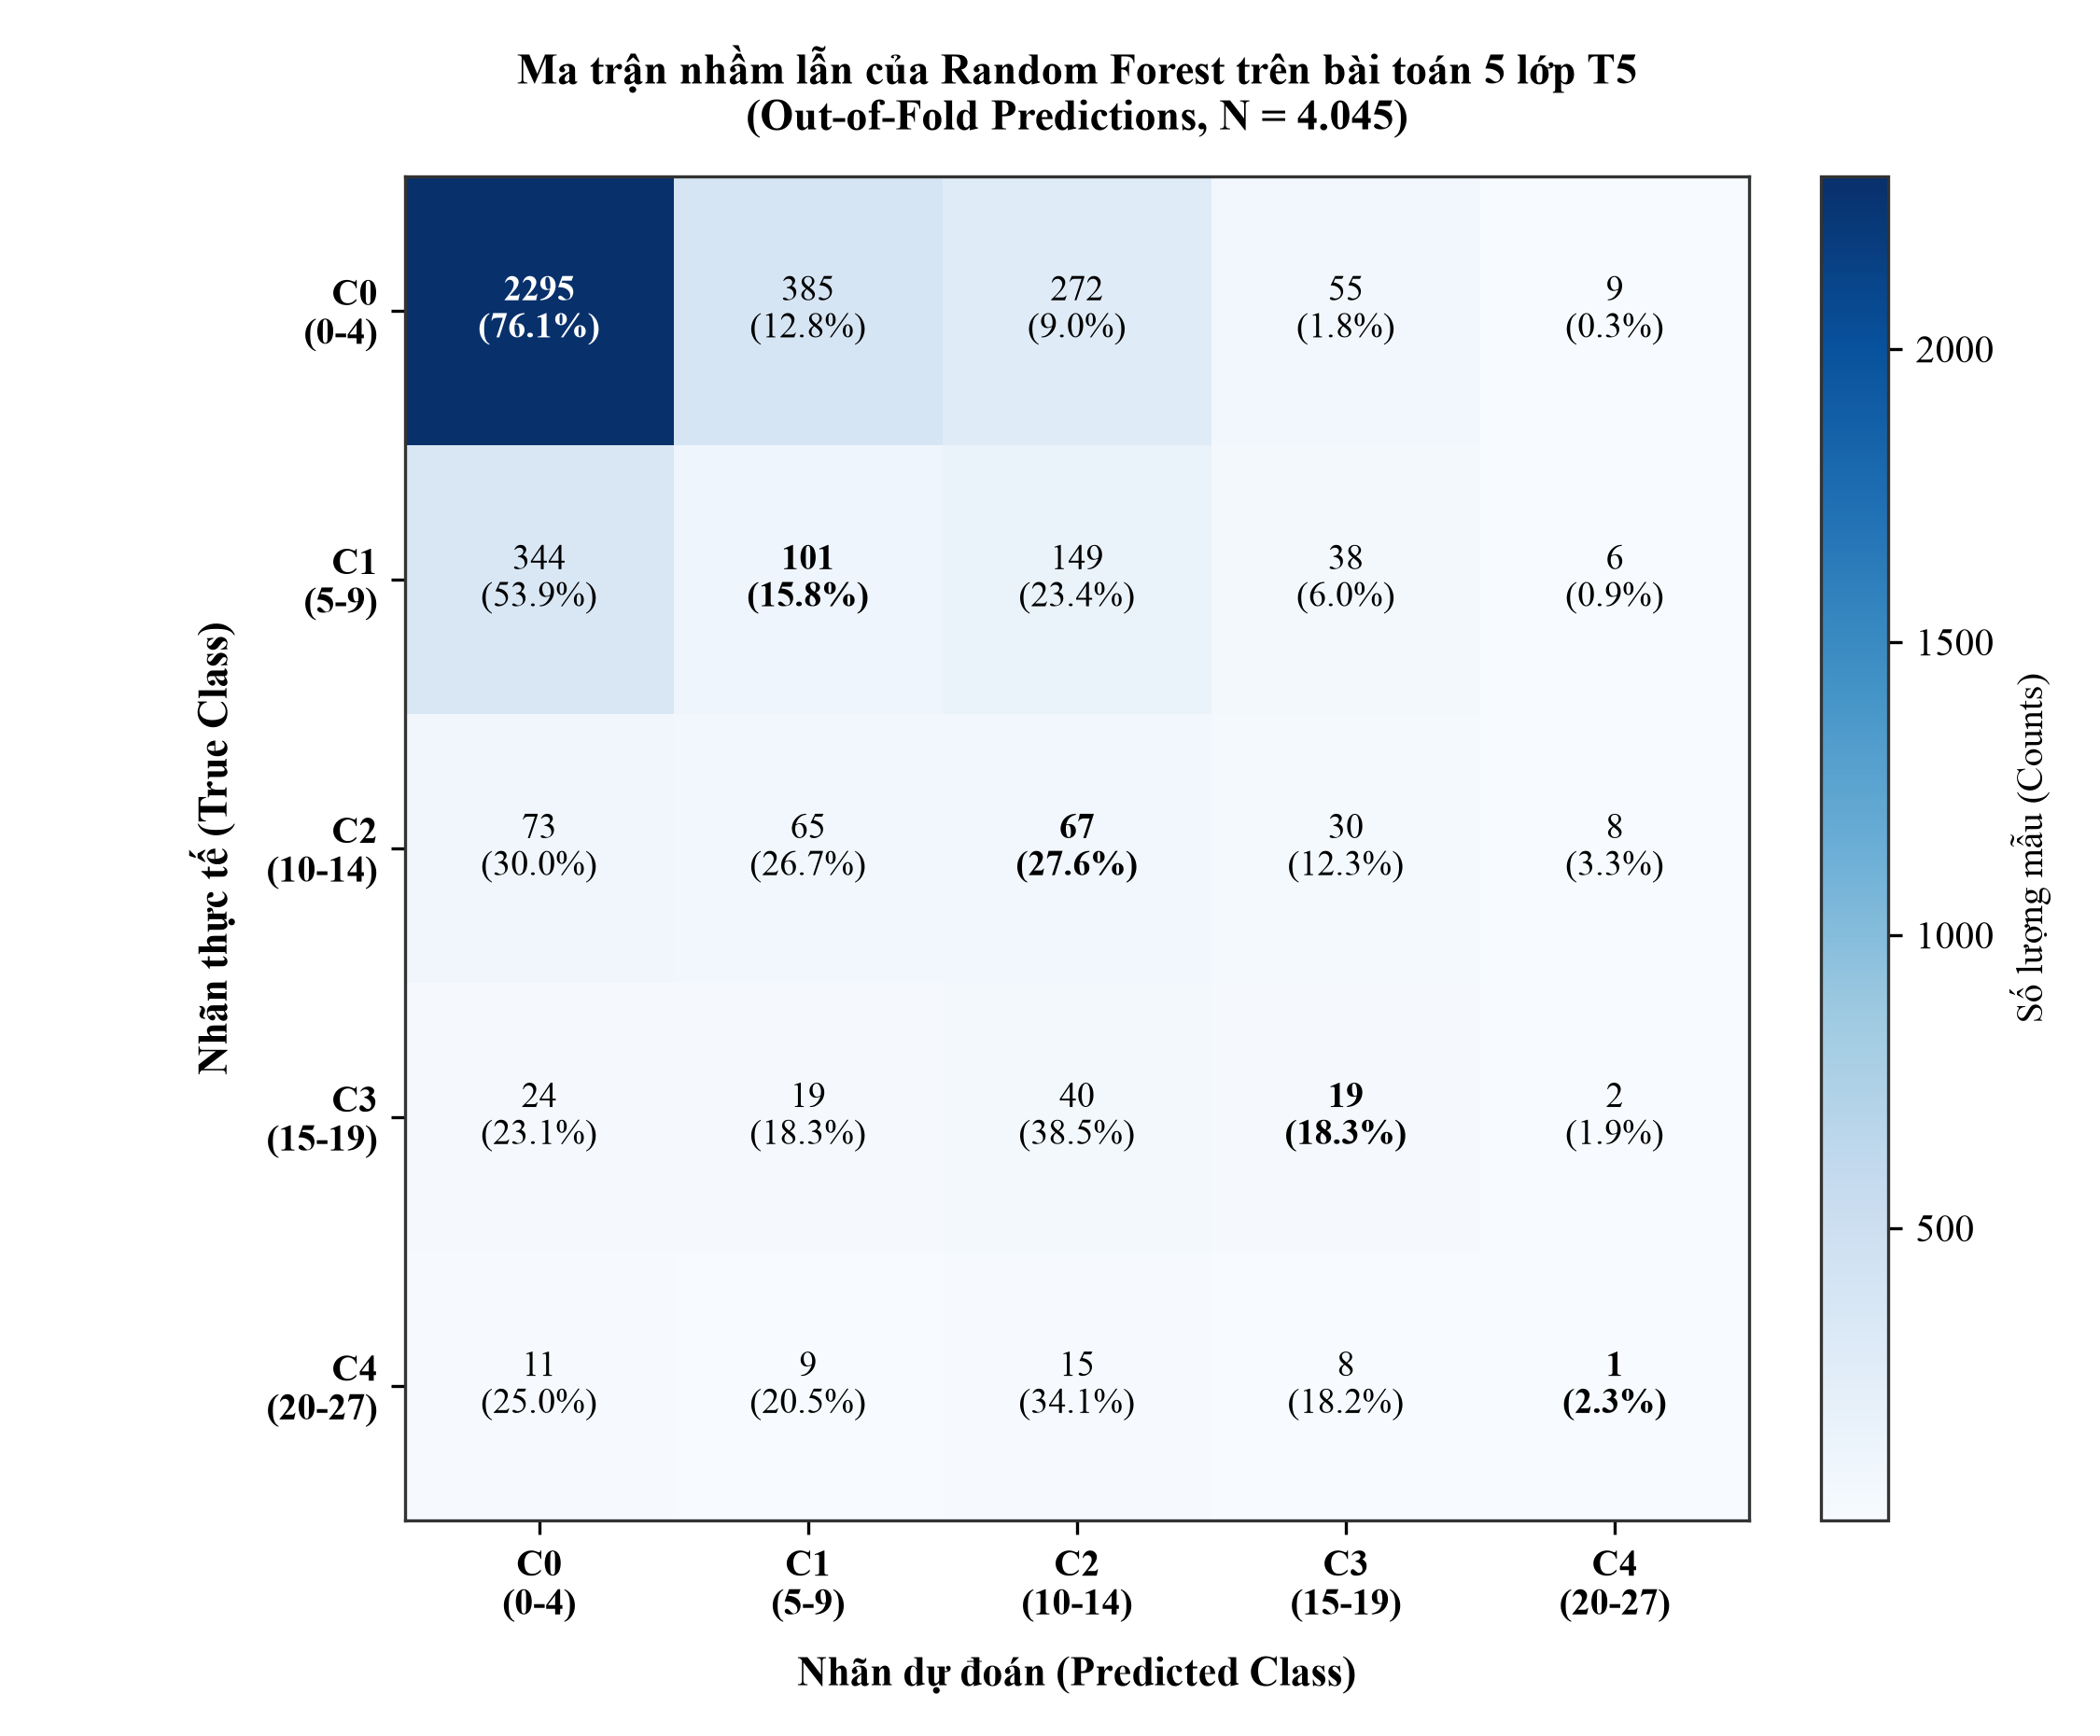
\includegraphics[width=0.75\textwidth]{figures/granularity_t5_confusion_matrix.png}
\label{fig:t5-confusion-matrix}
\end{figure}
\FloatBarrier

Ma trận nhầm lẫn $5 \times 5$ cho thấy: mô hình phân loại phẳng trên dữ liệu sinh lý ngoại vi có tỷ lệ nhận diện thấp ở lớp $C_4$ do cỡ mẫu rất nhỏ (44 mẫu trong tổng 4.045 quan sát), đồng thời có sự nhầm lẫn đáng kể giữa lớp $C_0$ và $C_1$. Các quan sát này đặt ra yêu cầu phải phân tích sâu hơn về đặc tính phân phối của các biến số đầu vào, đồng thời cung cấp cơ sở thực nghiệm quan trọng để nghiên cứu khảo sát thêm các hướng tiếp cận phân loại phân cấp và thứ bậc trên không gian 3 nhóm $T_3$.

\section{Phân tích đặc tính dữ liệu: Mức độ tương quan và chồng lấn phân phối đặc trưng}
\label{sec:phan-tich-chong-lan}

Để tìm hiểu các nguyên nhân dẫn đến đặc tính phân loại quan sát được ở Mục \ref{sec:target-granularity}, nghiên cứu tiến hành phân tích phân phối và mối liên hệ giữa các biến số với điểm số PHQ-9.

\subsection{Tương quan giữa các chỉ số cận lâm sàng và điểm PHQ-9}
Mức độ liên hệ giữa các biến đầu vào và tổng điểm PHQ-9 được thể hiện trong Hình \ref{fig:correlation-matrix}:
\begin{itemize}
    \item \textbf{Biến liên tục (Panel a):} Hệ số tương quan hạng Spearman ($\rho$) trích xuất từ dữ liệu thực nghiệm cho thấy nồng độ Albumin huyết thanh ($\rho = -0.164$), tỷ lệ thu nhập trên chuẩn nghèo PIR ($\rho = -0.159$) và thời lượng giấc ngủ ($\rho = -0.139$) có tương quan âm nhẹ với điểm PHQ-9; trong khi chỉ số khối cơ thể BMI ($\rho = +0.114$), chu vi vòng eo ($\rho = +0.095$), nhịp tim khi nghỉ ($\rho = +0.085$) và thời gian ngồi tĩnh tại ($\rho = +0.043$) có tương quan dương nhẹ.
    \item \textbf{Biến phân loại (Panel b):} Hệ số liên hệ Cramer's V ghi nhận tự đánh giá sức khỏe chung (HUQ010) có mức độ liên hệ cao nhất ($V = 0.195$), tiếp theo là giới tính ($V = 0.144$), hoạt động thể lực giải trí (PAQ665, $V = 0.125$), tiền sử tăng huyết áp (BPQ020, $V = 0.109$) và tiền sử đái tháo đường (DIQ010, $V = 0.100$).
\end{itemize}
Tất cả các hệ số tương quan và liên hệ đều ở mức khiêm tốn ($|\rho| \le 0.17$, $V \le 0.20$), chứng minh rằng không có bất kỳ biến sinh lý hay lâm sàng đơn lẻ nào mang tính quyết định để phân tách rạch ròi các mức độ triệu chứng.

\begin{figure}[htbp]{Mức độ tương quan và liên hệ giữa các đặc trưng đầu vào với điểm số PHQ-9: (a) Hệ số tương quan hạng Spearman $\rho$ của các biến liên tục; (b) Hệ số liên hệ Cramer's V của các biến phân loại}
\centering
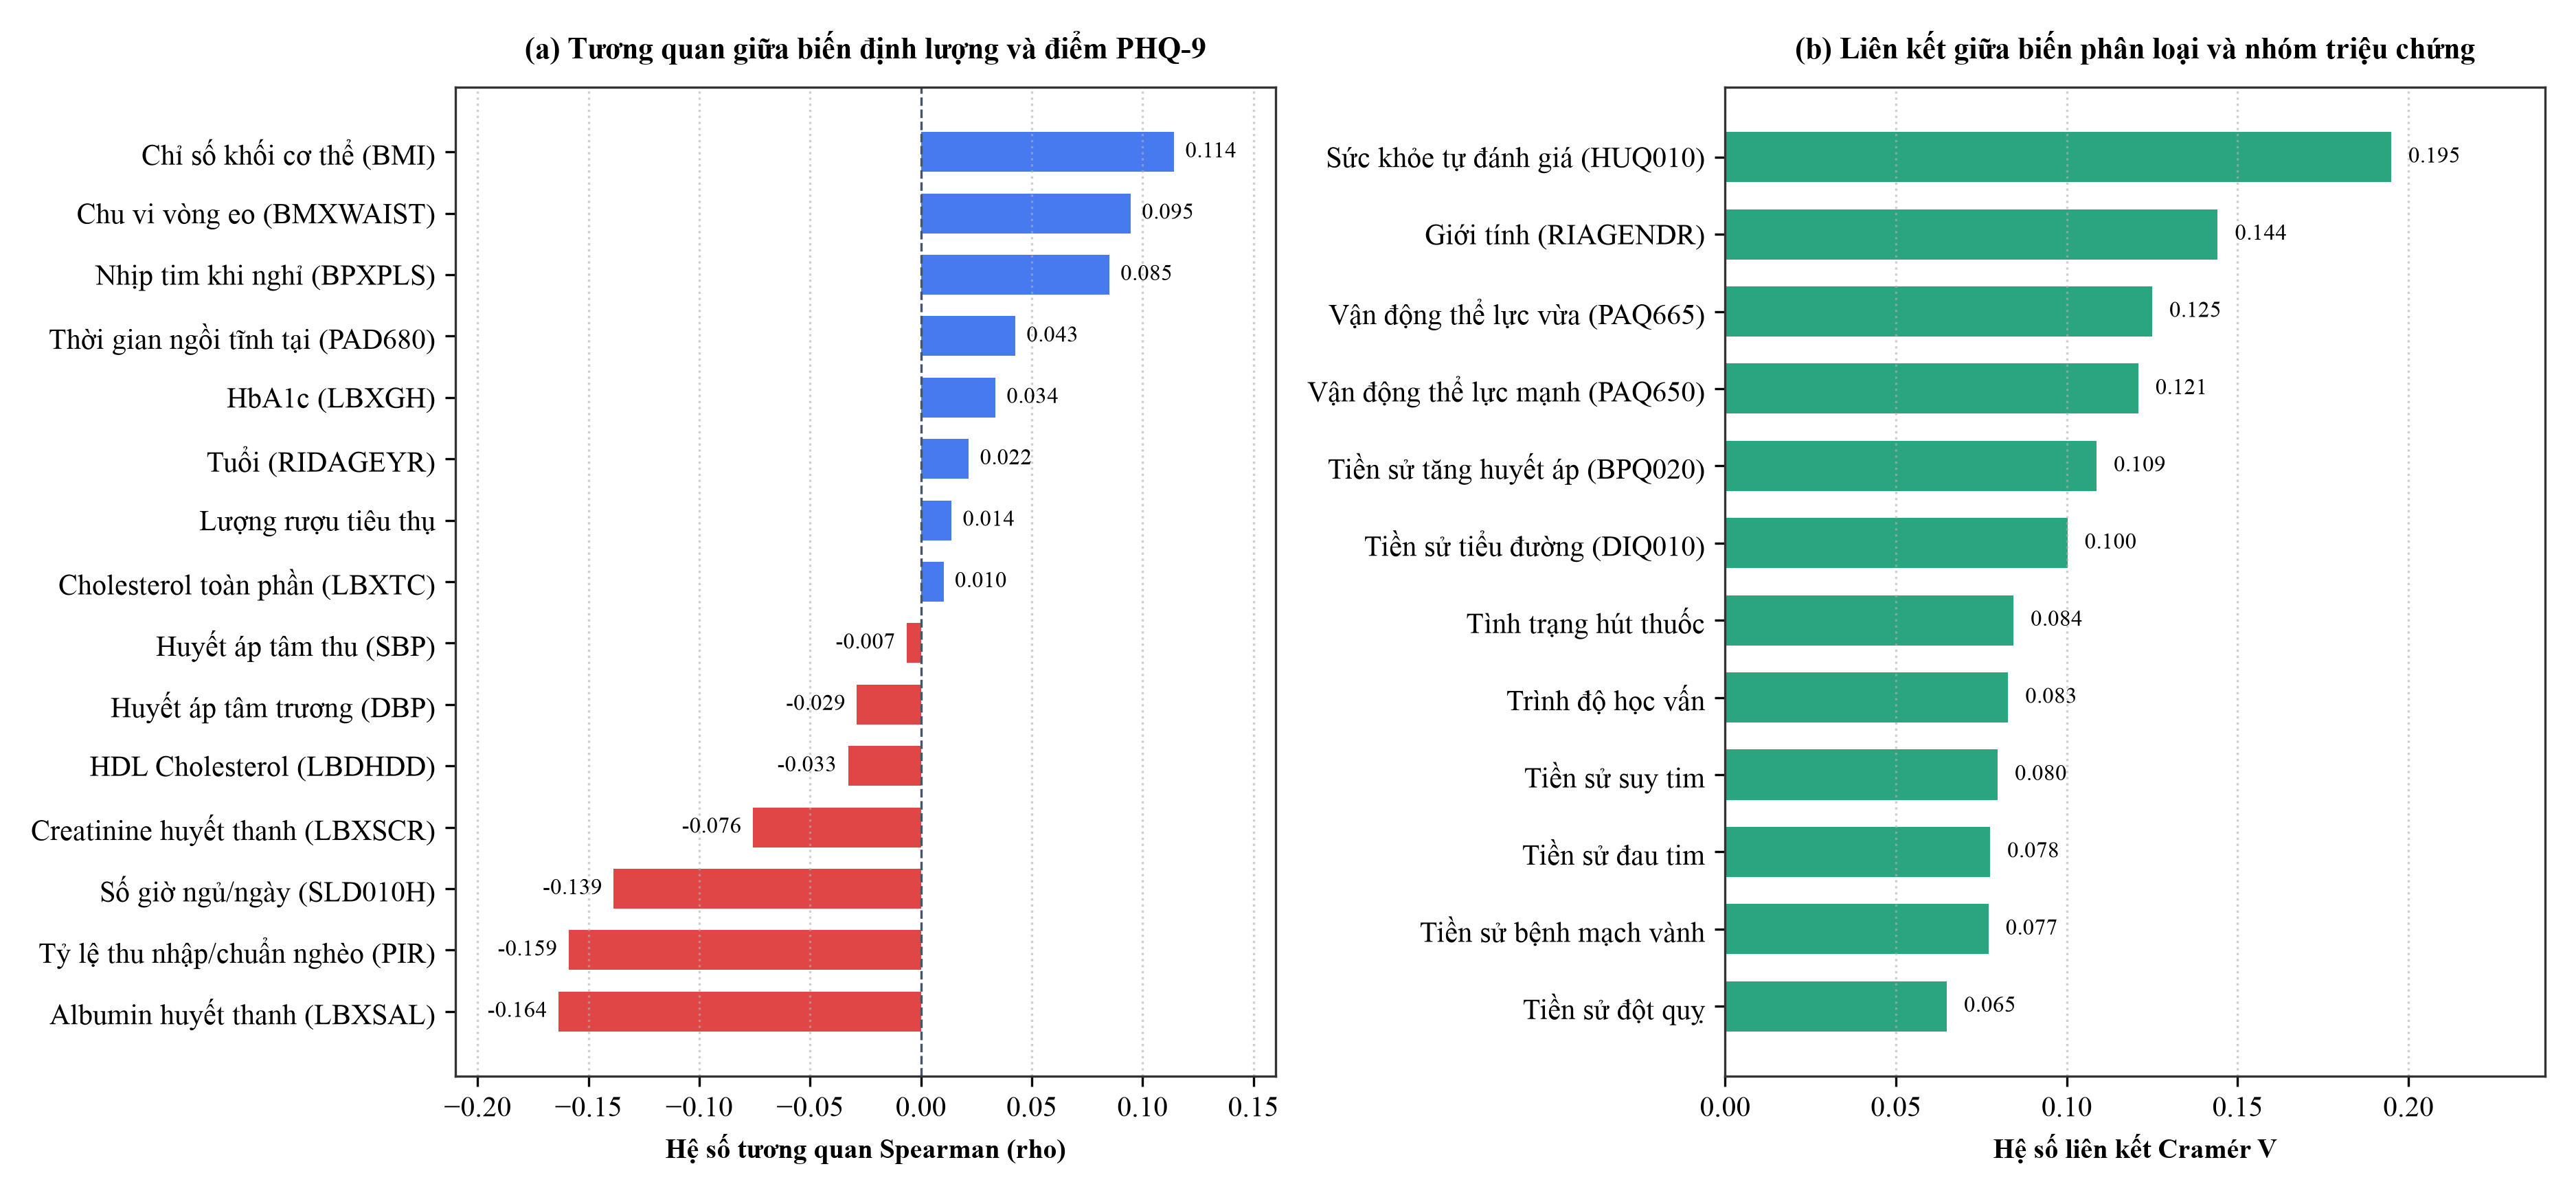
\includegraphics[width=0.92\textwidth]{figures/correlation_matrix.png}
\label{fig:correlation-matrix}
\end{figure}
\FloatBarrier

\subsection{Phân tích biểu đồ hộp và hình chiếu PCA}
Hình \ref{fig:overlap-boxplots} thể hiện phân bố giá trị của 6 chỉ số đặc trưng liên tục tiêu biểu (BMI, PIR, Giờ ngủ, Albumin, Nhịp tim, Thời gian ngồi tĩnh tại) qua các mức độ PHQ-9. Khoảng tứ phân vị (IQR) và trung vị của nhóm triệu chứng tối thiểu ($C_0$) và nhóm triệu chứng nhẹ ($C_1$) gần như trùng khớp nhau trên hầu hết các biến số (chẳng hạn trung vị BMI ở $C_0$ là 28.1 $\text{kg/m}^2$ so với 29.5 $\text{kg/m}^2$ ở $C_1$; Albumin ở $C_0$ là 43.0 g/L so với 42.0 g/L ở $C_1$; thời lượng ngủ trung vị cùng là 7.0 giờ). Sự phân tách chỉ bắt đầu thể hiện nhẹ ở nhóm triệu chứng nặng ($C_4$), tuy nhiên độ phân tán nội nhóm vẫn rất lớn.

\begin{figure}[htbp]{Biểu đồ hộp thể hiện sự tương đồng và chồng lấn phân phối của 6 biến sinh lý chính qua các mức độ PHQ-9}
\centering
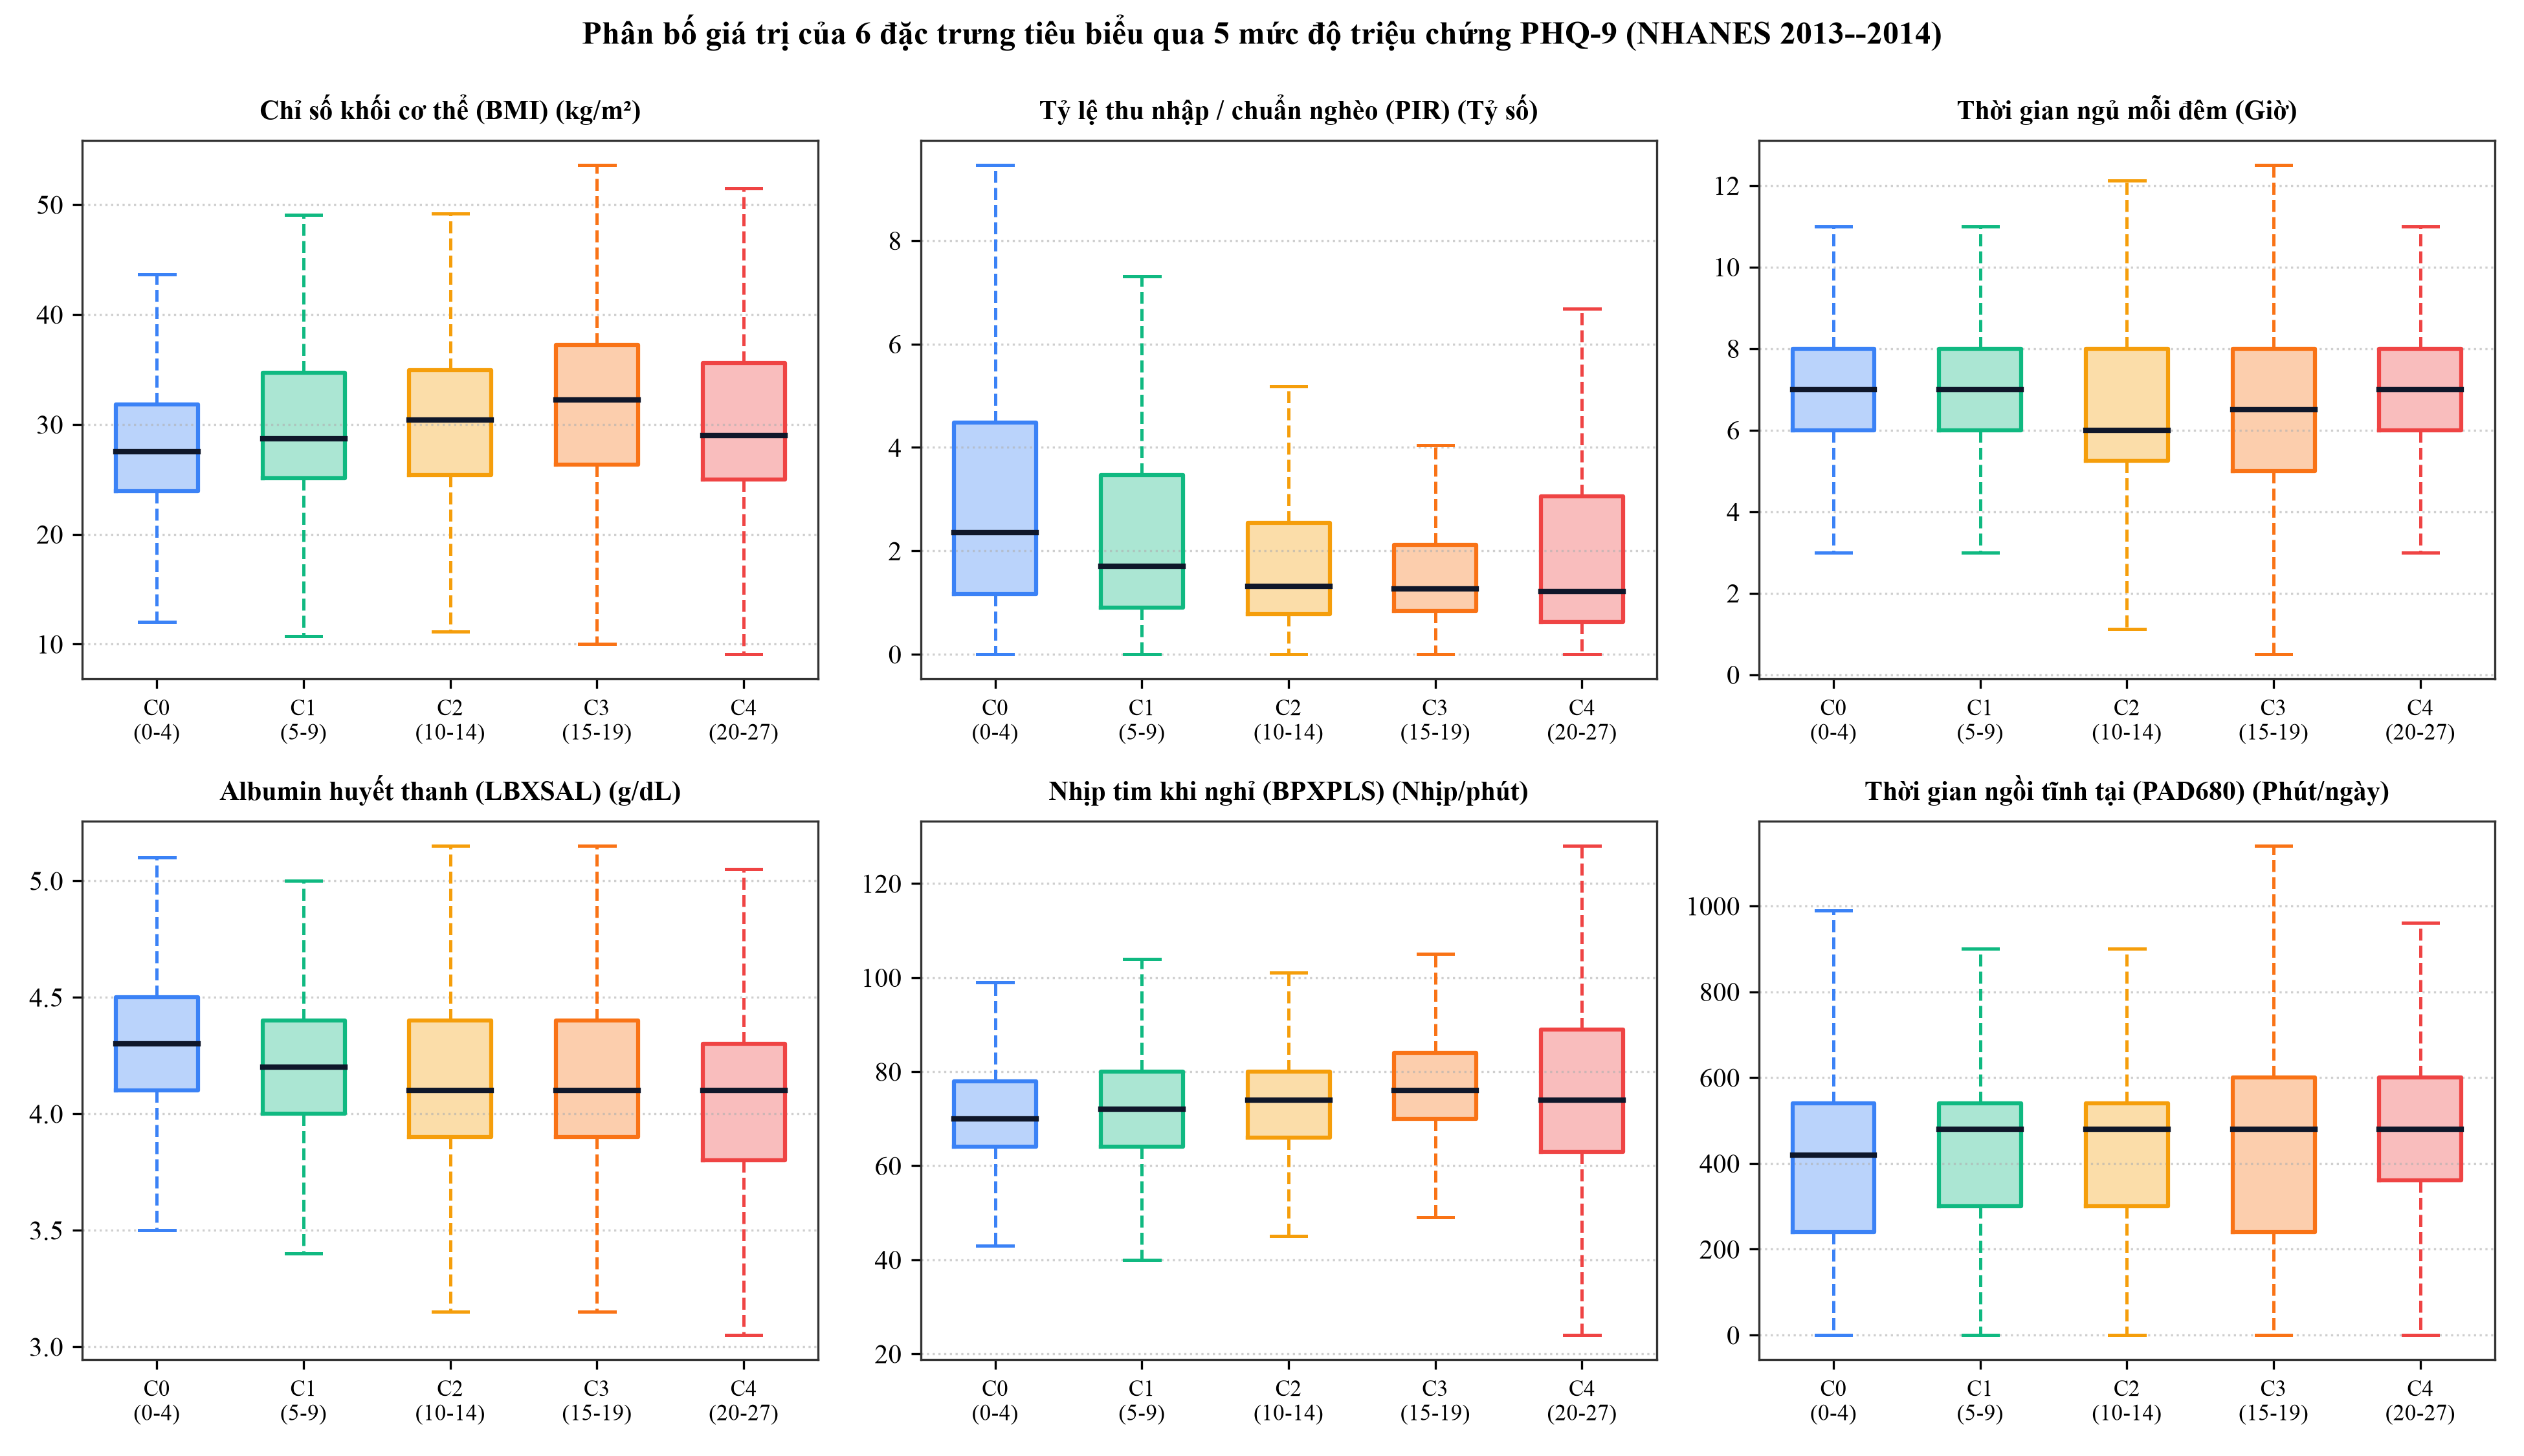
\includegraphics[width=0.92\textwidth]{figures/overlap_numerical_boxplots.png}
\label{fig:overlap-boxplots}
\end{figure}
\FloatBarrier

Khi chiếu không gian đặc trưng xuống mặt phẳng hai thành phần chính đầu tiên (PCA 2D, Hình \ref{fig:pca-overlap}), hai thành phần PC1 (12.3\%) và PC2 (8.8\%) giải thích tổng cộng 21.1\% phương sai dữ liệu. Cả trên không gian 5 mức độ $T_5$ (Panel a) lẫn không gian 3 nhóm $T_3$ (Panel b), đám mây điểm của nhóm $C_1$ lọt hoàn toàn vào bên trong đường bao mật độ của nhóm $C_0$. Nhóm nặng $C_4$ cũng không hình thành cụm tách biệt mà nằm phân tán rải rác.

Cần lưu ý rằng PCA là một phép chiếu tuyến tính hai chiều, không đại diện cho toàn bộ các tương tác phi tuyến phức tạp trong không gian đa chiều gốc. Dù vậy, hình chiếu PCA 2D trực quan hóa rõ nét hiện tượng chồng lấn phân phối sinh lý, giúp giải thích vì sao các mô hình học máy thường xuyên nhầm lẫn giữa các nhóm triệu chứng liền kề.

\begin{figure}[htbp]{Hình chiếu PCA 2D của không gian đặc trưng thể hiện sự chồng lấn phân phối: (a) Trên 5 mức độ $T_5$; (b) Trên 3 nhóm $T_3$}
\centering
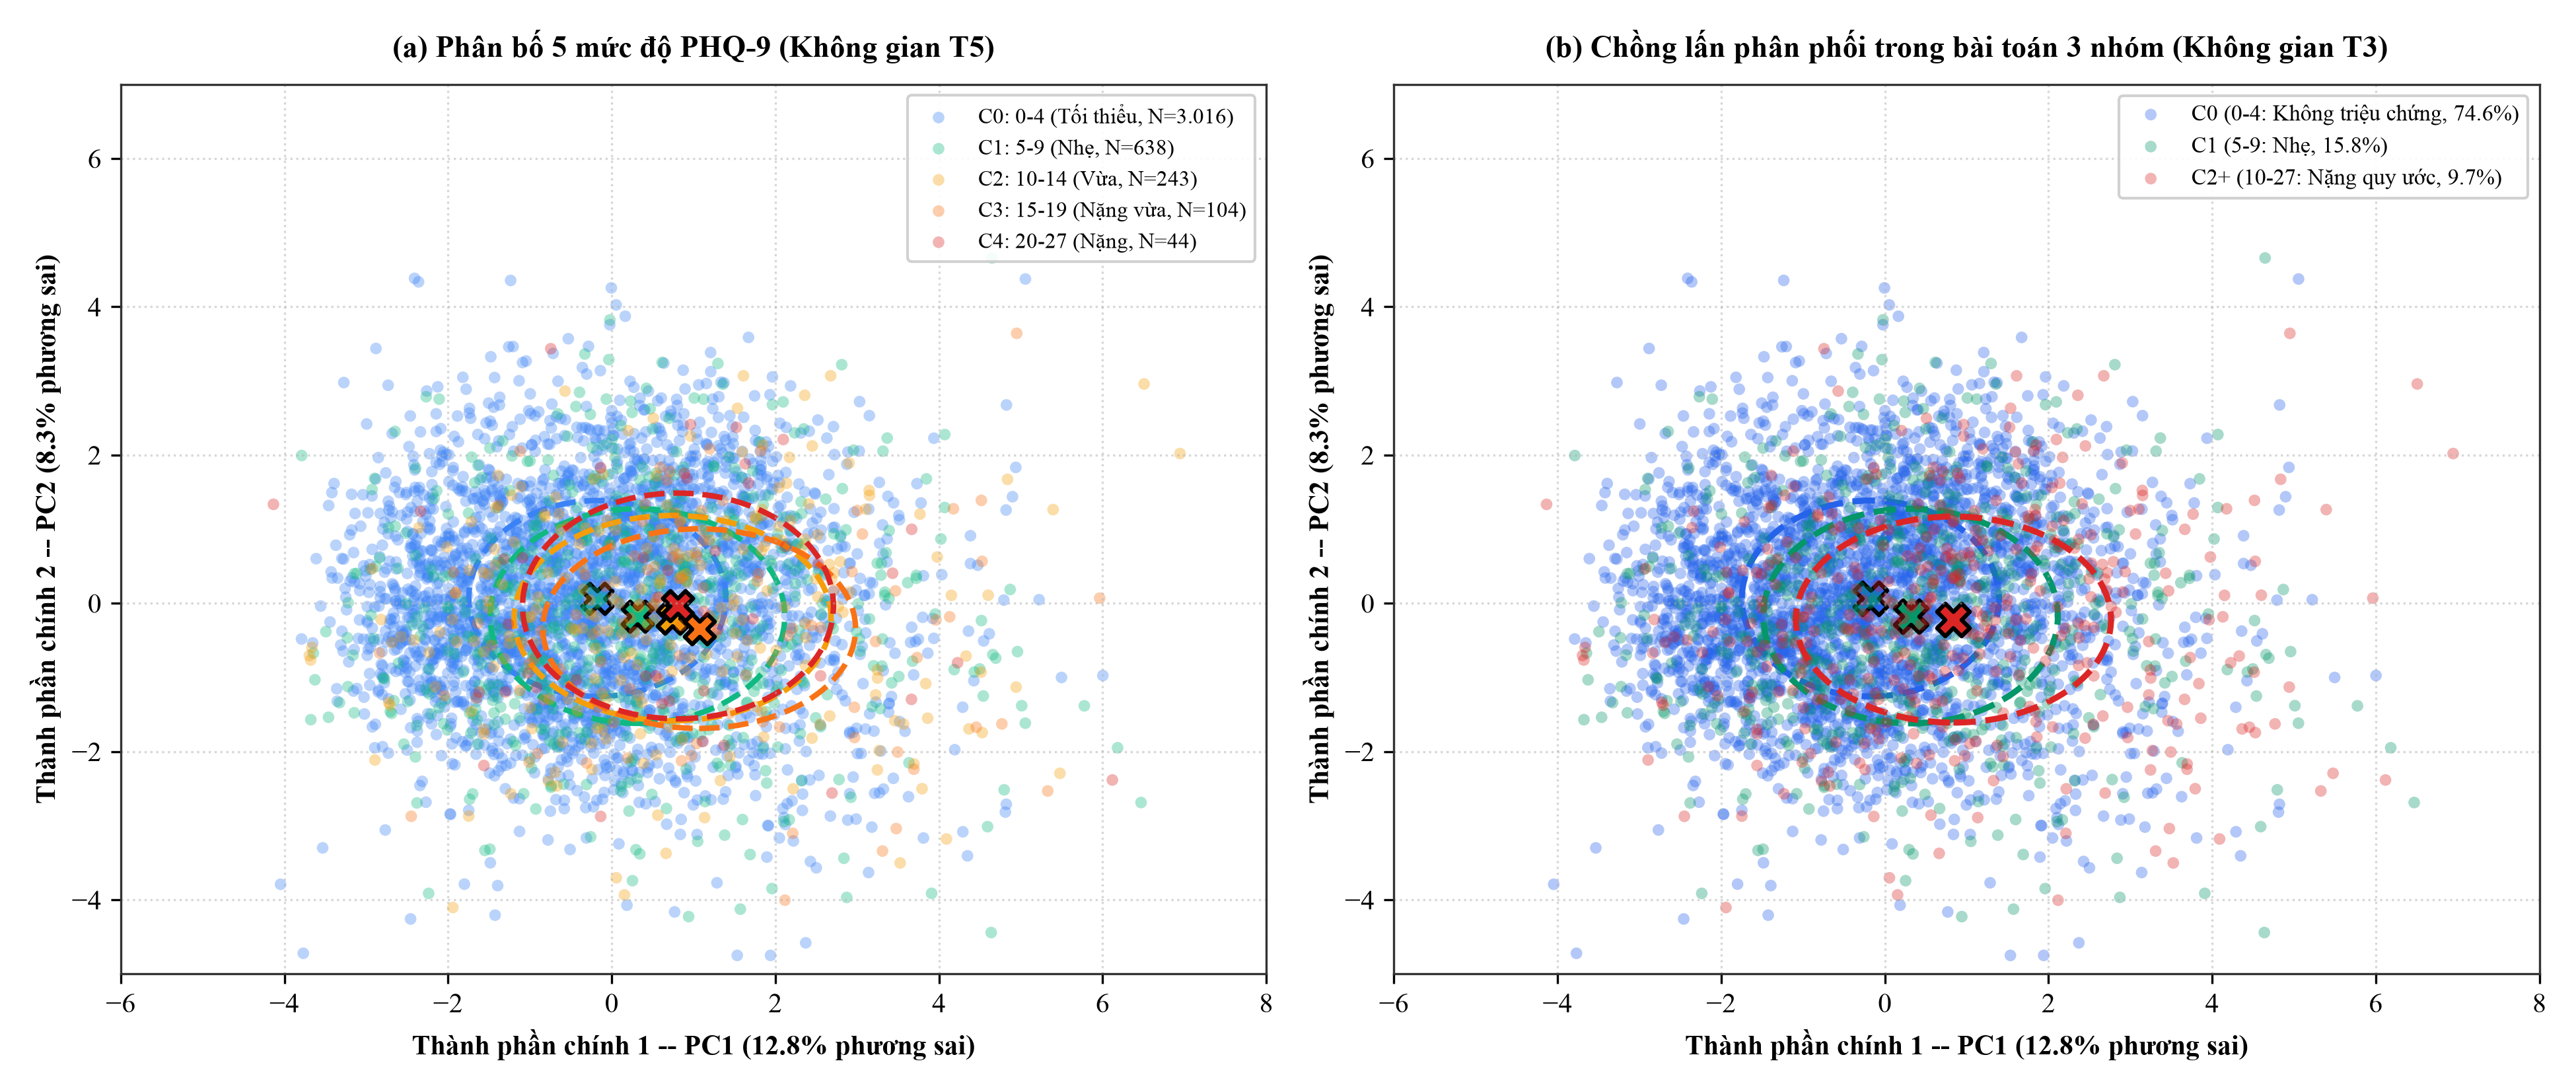
\includegraphics[width=0.92\textwidth]{figures/overlap_pca_C0_C4.png}
\label{fig:pca-overlap}
\end{figure}
\FloatBarrier

\section{Thử nghiệm mở rộng dữ liệu đa chu kỳ NHANES}
\label{sec:multicycle-results}

Để trả lời câu hỏi nghiên cứu \textbf{RQ3}, nghiên cứu tiến hành kiểm định trên tập dữ liệu gộp đa chu kỳ Pooled NHANES 2011--2016 ($N = 14.581$, tăng gấp 3.6 lần cỡ mẫu) với không gian 31 đặc trưng hài hòa ($F_{4\_\text{common31}}$).

Kết quả so sánh giữa chu kỳ đơn lẻ (Branch A, $N = 5.054$), tập dữ liệu gộp 3 chu kỳ (Branch B, $N = 14.581$) và kiểm định ngoại suy theo thời gian (Branch D, $N = 4.888$) qua các mức độ chi tiết nhãn ($T_2 \to T_5$) được thể hiện trong Hình \ref{fig:multicycle-cohort-comparison}.

\begin{figure}[htbp]{So sánh Macro-F1 và Balanced Accuracy theo độ chi tiết nhãn giữa chu kỳ đơn lẻ (Branch A), tập dữ liệu gộp (Branch B) và kiểm định thời gian (Branch D)}
\centering
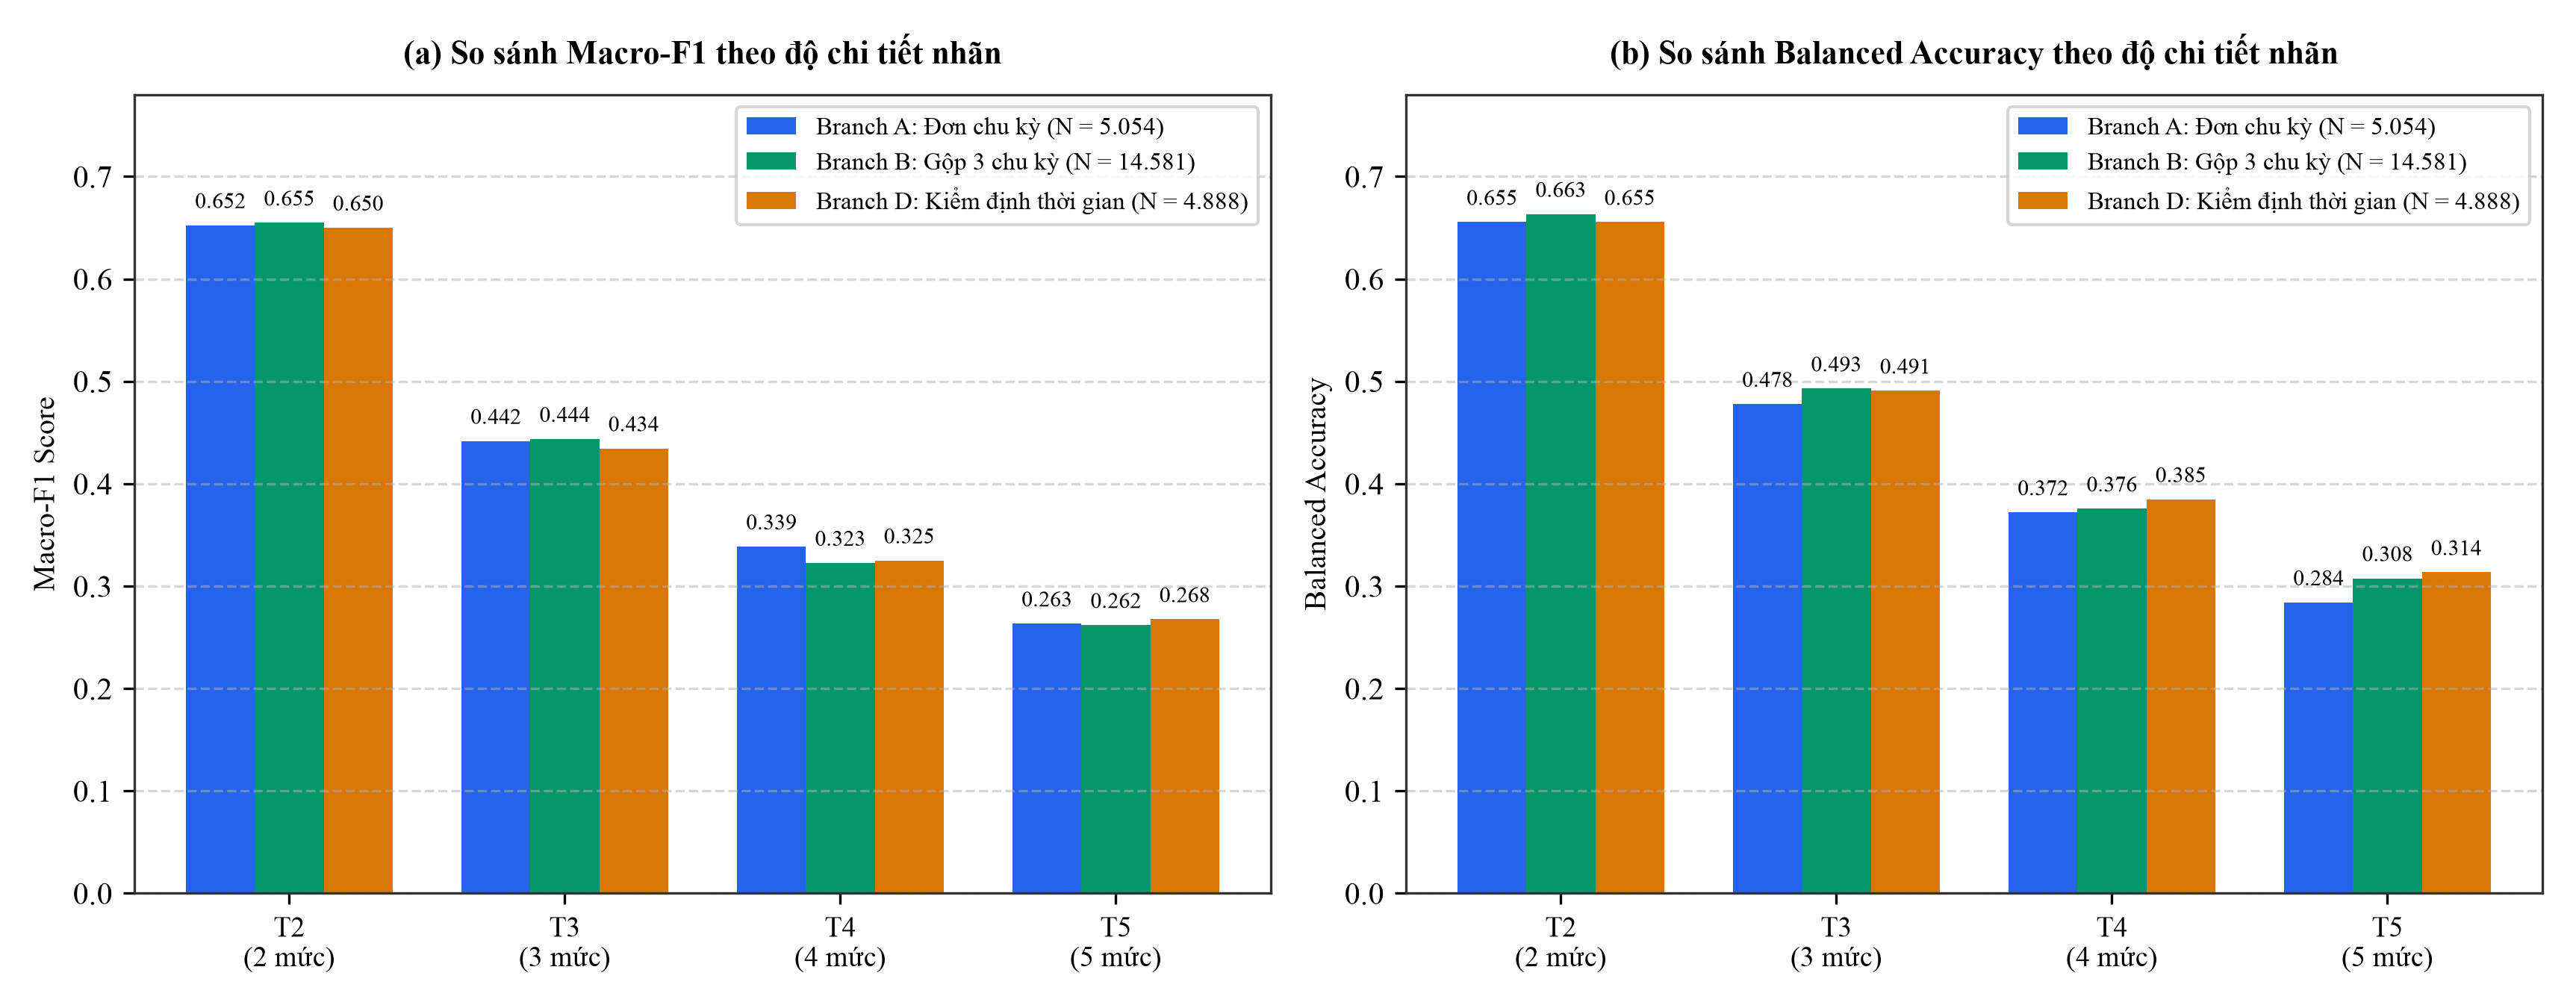
\includegraphics[width=\textwidth]{figures/multicycle_cohort_comparison.png}
\label{fig:multicycle-cohort-comparison}
\end{figure}
\FloatBarrier

Kết quả thực nghiệm cho thấy:
\begin{itemize}
    \item Việc tăng cỡ mẫu lên $14.581$ đối tượng giúp cải thiện nhẹ Balanced Accuracy trên nhiệm vụ 5 mức $T_5$ (tăng từ 0.2841 lên 0.3076).
    \item Tuy nhiên, Macro-F1 trên $T_5$ không có sự cải thiện rõ rệt (0.2634 ở Branch A so với 0.2619 ở Branch B).
\end{itemize}
Kết quả này cho thấy khi dữ liệu gặp hiện tượng chồng lấn phân phối giữa các nhóm triệu chứng, việc chỉ gia tăng cỡ mẫu đơn thuần mà không bổ sung thêm các chiều đặc trưng có độ đặc hiệu cao hơn khó có thể tạo ra bước nhảy vọt về hiệu năng phân loại trên bài toán 5 mức.

\section{Mở rộng khảo sát: Kết nối từ bài toán đa mức $T_5$ sang phân loại phân cấp và thứ bậc $T_3$}
\label{sec:chuyen-dich-t5-t3}

Các chuỗi thực nghiệm trên không gian 5 lớp $T_5$ đã mang lại nhiều hiểu biết có giá trị về đặc tính dữ liệu và hành vi của các mô hình học máy:
\begin{enumerate}
    \item \textbf{Đóng góp tích cực của các nhóm đặc trưng:} Việc mở rộng từ các chỉ số xét nghiệm và thể chất đơn thuần ($F_1$) sang không gian tích hợp tiền sử bệnh lý, lối sống và nhân khẩu học ($F_4$) nâng rõ rệt Macro-F1 trên từng thuật toán (như XGBoost tăng từ 0.2173 lên 0.2707; Random Forest tăng từ 0.2052 lên 0.2232; Logistic Regression tăng từ 0.1900 lên 0.2152), chứng minh các yếu tố hành vi và nhân khẩu học cung cấp tín hiệu bổ trợ quan trọng cho phân tầng nguy cơ.
    \item \textbf{Đặc tính phân phối sinh lý ngoại vi:} Phân tích tương quan hạng Spearman, liên hệ Cramer's V và biểu đồ hình chiếu PCA 2D đã chỉ ra rằng các chỉ số sinh lý ngoại vi giữa nhóm triệu chứng tối thiểu ($C_0$) và triệu chứng nhẹ ($C_1$) có độ tương đồng và chồng lấn phân phối rất lớn. Đây là đặc điểm khách quan của các biến số dạng bảng trích xuất từ khảo sát sức khỏe cộng đồng.
    \item \textbf{Khảo sát quy mô mẫu:} Việc mở rộng cỡ mẫu lên 14.581 quan sát qua 3 chu kỳ NHANES giúp ổn định Balanced Accuracy (tăng từ 0.2841 lên 0.3076) nhưng không làm tăng đáng kể Macro-F1 trên $T_5$, khẳng định rằng đặc tính phân tách của bài toán phụ thuộc chủ yếu vào mức độ đặc hiệu của tập biến số hơn là số lượng mẫu quan sát.
\end{enumerate}

Trong bối cảnh sàng lọc sức khỏe tâm thần ban đầu, bên cạnh bài toán phân loại chi tiết 5 mức độ, một nhu cầu thực tế thường được quan tâm là phân tầng đối tượng theo hai bước ra quyết định rõ ràng:
\begin{itemize}
    \item \textit{Bước 1 (Nhận diện triệu chứng):} Phân biệt giữa người có triệu chứng tối thiểu ($C_0$, điểm 0--4) và người có biểu hiện triệu chứng cần lưu ý ($C_{12}$, điểm 5--27).
    \item \textit{Bước 2 (Phân tầng mức độ):} Trong nhóm người có triệu chứng, phân biệt giữa mức nhẹ ($C_1$, điểm 5--9) và mức nặng theo quy ước nghiên cứu ($C_2^+$, điểm 10--27).
\end{itemize}

Do đó, các phát hiện thực nghiệm trên $T_5$ đóng vai trò là cơ sở khoa học để nghiên cứu \textbf{mở rộng khảo sát sang bài toán 3 nhóm ($T_3$)} và đánh giá có hệ thống 8 cấu hình mô hình thực nghiệm ($E_0 \to E_7$) đại diện cho các hướng tiếp cận phẳng, phân cấp cứng, phân cấp mềm kết hợp chi phí Bayes và phân loại thứ bậc. Cần nhấn mạnh rằng $T_3$ và $T_5$ là hai bài toán phân loại độc lập với không gian nhãn và mục tiêu ứng dụng khác nhau; việc khảo sát song song cả hai bài toán giúp cung cấp bức tranh hoàn chỉnh về đặc điểm của các mô hình học máy trên dữ liệu sinh lý dạng bảng.

\begin{figure}[htbp]{Tổng hợp kết quả khảo sát trên hai hướng thực nghiệm: Phân loại đa mức $T_5$ và các hướng mô hình hóa trên $T_3$}
\centering
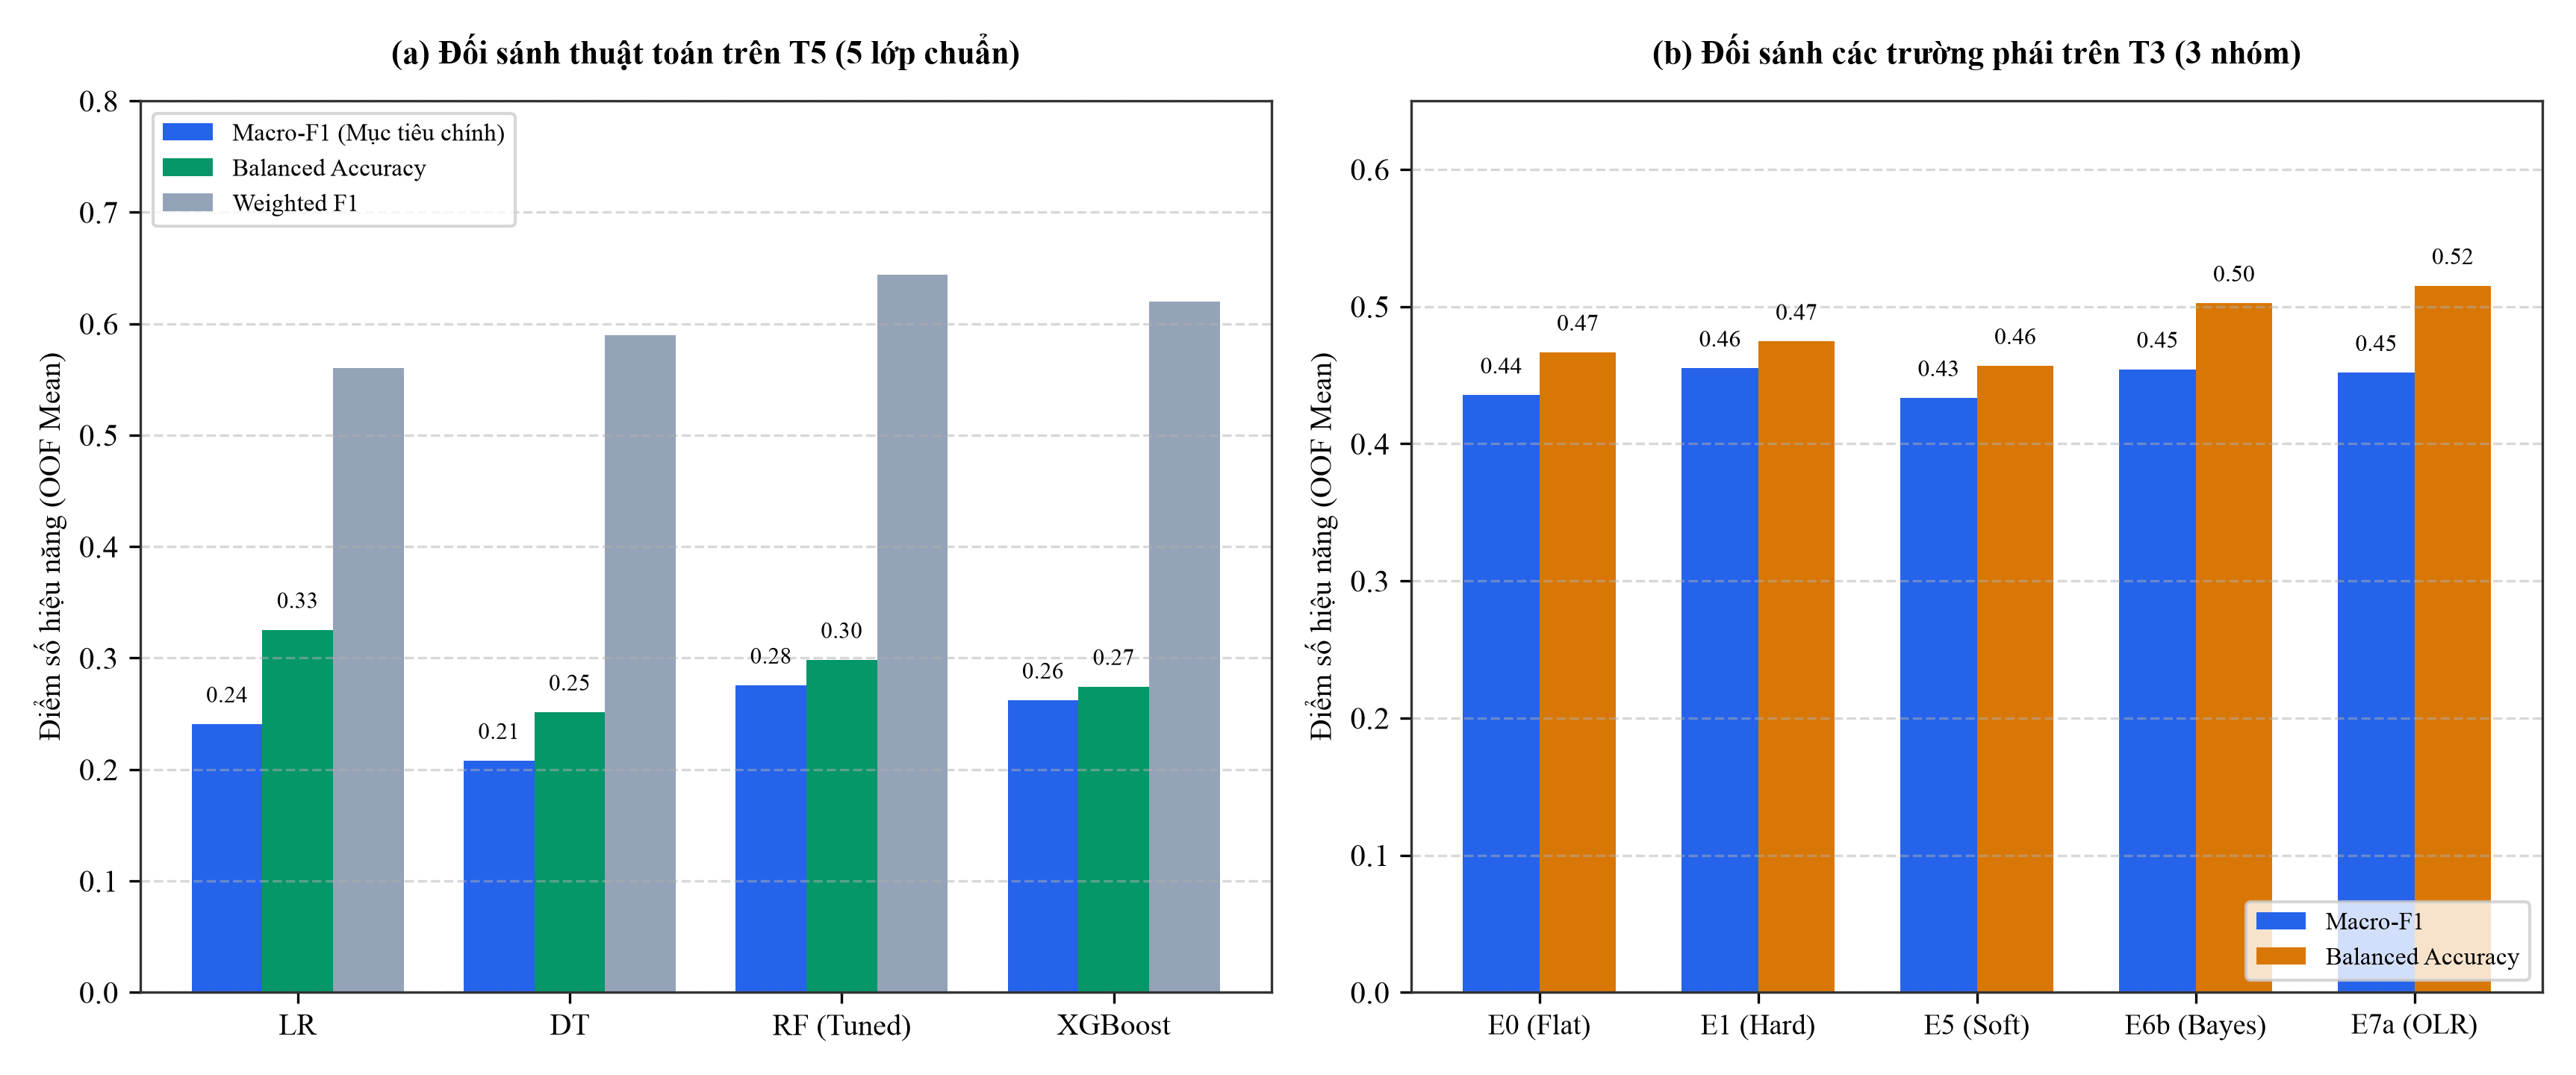
\includegraphics[width=\textwidth]{figures/fig4_algorithm_comparison_t5_t3.png}
\label{fig:algo-comparison-t5-t3}
\end{figure}
\FloatBarrier

\section{Khảo sát các hướng tiếp cận mô hình hóa trên không gian 3 nhóm ($T_3$): Đánh giá $E_0 \to E_7$}
\label{sec:khao-sat-e0-e7}

Trên không gian 3 nhóm ($T_3$: $C_0, C_1, C_2^+$), nghiên cứu khảo sát có hệ thống 8 cấu hình mô hình thực nghiệm ($E_0 \to E_7$) trên tập phát triển Legacy ($N = 4.045$).

\subsection{Kết quả các cấu hình phân cấp cứng ($E_1 \to E_3$)}
Kiến trúc phân cấp cứng chia bài toán thành hai bộ phân loại nhị phân nối tiếp: Stage 1 sàng lọc $C_0$ vs $C_{12}$; Stage 2 phân tầng $C_1$ vs $C_2^+$.
\begin{itemize}
    \item \textbf{Cơ chế huấn luyện in-fold:} Bộ phân loại Stage 1 được huấn luyện trên toàn bộ dữ liệu huấn luyện của fold. Bộ phân loại Stage 2 được huấn luyện \textbf{chỉ trên các mẫu trong fold có nhãn thật $\text{PHQ-9} \ge 5$} ($N = 1.029$ ca trên toàn bộ tập phát triển).
    \item \textbf{Cơ chế suy luận ngoài mẫu:} Nếu Stage 1 dự đoán một mẫu là $C_0$, mẫu được gán nhãn $C_0$ ngay lập tức. Chỉ các mẫu được dự đoán là $C_{12}$ mới được chuyển sang Stage 2.
\end{itemize}

Kết quả thực nghiệm out-of-fold của các mô hình phân cấp cứng được trình bày trong Bảng \ref{tab:hard-hierarchical-results}.

\begin{table}{So sánh hiệu năng giữa Flat Classification và Hard Hierarchical trên nhiệm vụ $T_3$ ($N = 4.045$)}
\centering
\footnotesize
\setlength{\tabcolsep}{3pt}
\label{tab:hard-hierarchical-results}
\begin{tabularx}{\textwidth}{l >{\centering\arraybackslash}X >{\centering\arraybackslash}X >{\centering\arraybackslash}X >{\centering\arraybackslash}X >{\centering\arraybackslash}X >{\centering\arraybackslash}X}
\toprule
\textbf{Mô hình} & \textbf{Macro-F1 (Mean $\pm$ SD)} & \textbf{BalAcc} & \textbf{Accuracy} & \textbf{Recall $C_1$} & \textbf{Recall $C_2^+$} & \textbf{Bỏ sót $C_2^+ \to C_0$} \\
\midrule
$E_0$ (Flat RF)       & 0.4354 $\pm$ 0.0075 & 0.4667 & 64.10\% & 16.29\% & 47.32\% & 108 ca \\
$E_1$ (Hard RF--RF)   & 0.4550 $\pm$ 0.0056 & 0.4745 & 68.08\% & 16.46\% & 43.74\% & 120 ca \\
$E_2$ (Hard Tuned)    & \textbf{0.4586 $\pm$ 0.0124} & 0.4745 & 65.32\% & \textbf{25.69\%} & 39.63\% & \textbf{98 ca} \\
$E_3a$ (Hard RF--LR)  & 0.4567 $\pm$ 0.0271 & \textbf{0.4964} & \textbf{68.43\%} & 11.75\% & \textbf{55.00\%} & 120 ca \\
$E_3b$ (Hard RF--XGB) & 0.4575 $\pm$ 0.0182 & 0.4790 & 68.23\% & 16.77\% & 44.76\% & 120 ca \\
\bottomrule
\end{tabularx}

\vspace{0.15cm}
\raggedright
\scriptsize
\textit{Ghi chú:} Số ca bỏ sót $C_2^+ \to C_0$ là số lượng tổng hợp từ toàn bộ dự đoán ngoài mẫu (pooled out-of-fold, $N = 4.045$).
\end{table}


\textbf{Phân tích kết quả phân cấp cứng:}
\begin{enumerate}
    \item \textbf{Cải thiện Macro-F1:} Cấu hình phân cấp cứng $E_1$ (Hard RF--RF) đạt Macro-F1 = \textbf{0.4550 $\pm$ 0.0056}, cải thiện so với mô hình phẳng $E_0$ (0.4354). Cấu hình tối ưu siêu tham số $E_2$ (Hard RF--RF Tuned) nâng Macro-F1 lên mức cao nhất trong nhóm khảo sát là \textbf{0.4586 $\pm$ 0.0124}.
    \item \textbf{Đặc điểm lan truyền sai số và tỷ lệ bỏ sót ca nặng:} Trong mô hình $E_1$, có \textbf{120 ca nặng ($C_2^+$) bị Stage 1 dự đoán nhầm thành $C_0$} (tương đương 30.69\% tổng số 391 ca nặng). Khi đã bị Stage 1 gán nhãn $C_0$, các ca này kết thúc luồng dự đoán và không được Stage 2 tiếp cận. Cấu hình tối ưu siêu tham số $E_2$ giảm số ca này xuống còn \textbf{98 ca}. Con số này phản ánh đặc tính cơ học của định tuyến cứng: quyết định loại trừ ở giai đoạn 1 mang tính một chiều và không thể đảo ngược ở giai đoạn 2.
\end{enumerate}

\subsection{Kết quả các cấu hình phân cấp mềm và Quyết định nhạy chi phí ($E_4 \to E_6$)}
Nhằm linh hoạt điều chỉnh quy tắc quyết định và tận dụng phân phối xác suất liên tục giữa hai giai đoạn, các mô hình phân cấp mềm ($E_4, E_5$) kết hợp phân phối xác suất qua công thức xác suất toàn phần. Kết quả được trình bày trong Bảng \ref{tab:soft-cost-results}.

\begin{table}{Hiệu năng mô hình Soft Hierarchical và Quyết định Nhạy chi phí trên nhiệm vụ $T_3$ ($N = 4.045$)}
\centering
\footnotesize
\setlength{\tabcolsep}{3pt}
\label{tab:soft-cost-results}
\begin{tabularx}{\textwidth}{l >{\centering\arraybackslash}X >{\centering\arraybackslash}X >{\centering\arraybackslash}X >{\centering\arraybackslash}X >{\centering\arraybackslash}X >{\centering\arraybackslash}X >{\centering\arraybackslash}X}
\toprule
\textbf{Mô hình} & \textbf{Macro-F1} \newline \textbf{(Mean $\pm$ SD)} & \textbf{BalAcc} & \textbf{Accuracy} & \textbf{Recall $C_1$} & \textbf{Recall $C_2^+$} & \textbf{Bỏ sót} \newline \textbf{$C_2^+ \to C_0$} & \textbf{Báo động} \newline \textbf{$C_0 \to C_2^+$} \\
\midrule
$E_4$ (Soft RF--RF) & 0.4206 $\pm$ 0.0104 & 0.4309 & \textbf{73.75\%} & 5.18\% & 30.19\% & 227 ca & \textbf{139 ca} \\
$E_5$ (Soft RF--LR) & 0.4270 $\pm$ 0.0118 & 0.4506 & 73.37\% & 3.45\% & 39.13\% & 211 ca & 176 ca \\
$E_{6a}$ (Soft Cost RF--RF) & \textbf{0.4535 $\pm$ 0.0149} & 0.4904 & 56.91\% & \textbf{40.92\%} & 44.25\% & \textbf{62 ca} & 215 ca \\
$E_{6b}$ (Soft Cost RF--LR) & 0.4521 $\pm$ 0.0190 & \textbf{0.5025} & 56.84\% & 34.64\% & \textbf{54.23\%} & \textbf{62 ca} & 294 ca \\
\bottomrule
\end{tabularx}

\vspace{0.15cm}
\raggedright
\scriptsize
\textit{Ghi chú:} Macro-F1, BalAcc, Accuracy và Recall là trung bình qua 5 folds. Số ca bỏ sót và báo động là số lượng tổng hợp từ toàn bộ dự đoán ngoài mẫu (pooled out-of-fold, $N = 4.045$).
\end{table}


Để chủ động kiểm soát tỷ lệ bỏ sót ca nặng, cấu hình tối ưu chi phí Bayes $E_{6b}$ (Soft Cost RF--LR với ma trận chi phí $M_1$, đặt mức phạt bỏ sót ca nặng $\mathbf{C}(2, 0) = 3.0$) đưa hàm rủi ro kỳ vọng vào quy tắc quyết định. Kết quả thực nghiệm: $E_{6b}$ đạt Balanced Accuracy là \textbf{0.5025 $\pm$ 0.0163} và Macro-F1 = \textbf{0.4521 $\pm$ 0.0190}, đồng thời giảm số ca nặng bị bỏ sót thành bình thường ($C_2^+ \to C_0$) từ 120 ca ($E_1$) xuống còn \textbf{62 ca} (Hình \ref{fig:confusion-error-analysis}a), tương đương mức giảm \textbf{48.33\%} (tỷ lệ bỏ sót giảm từ 30.69\% xuống 15.86\%). Khi áp dụng ma trận phạt cao hơn $M_2$ ($\mathbf{C}(2, 0) = 5.0$), số ca bỏ sót giảm tiếp xuống còn \textbf{19 ca} (giảm 84.17\%), và với $M_3$ ($\mathbf{C}(2, 0) = 8.0$) chỉ còn \textbf{7 ca} (giảm 94.17\%), đổi lại số lượng báo động nhầm từ lớp bình thường tăng lên tương ứng.

\begin{figure}[htbp]{(a) Số ca nặng bị phân loại nhầm thành bình thường ($C_2^+ \to C_0$) và (b) So sánh Recall từng lớp giữa $E_1, E_{6b}$ và $E_{7a}$}
\centering
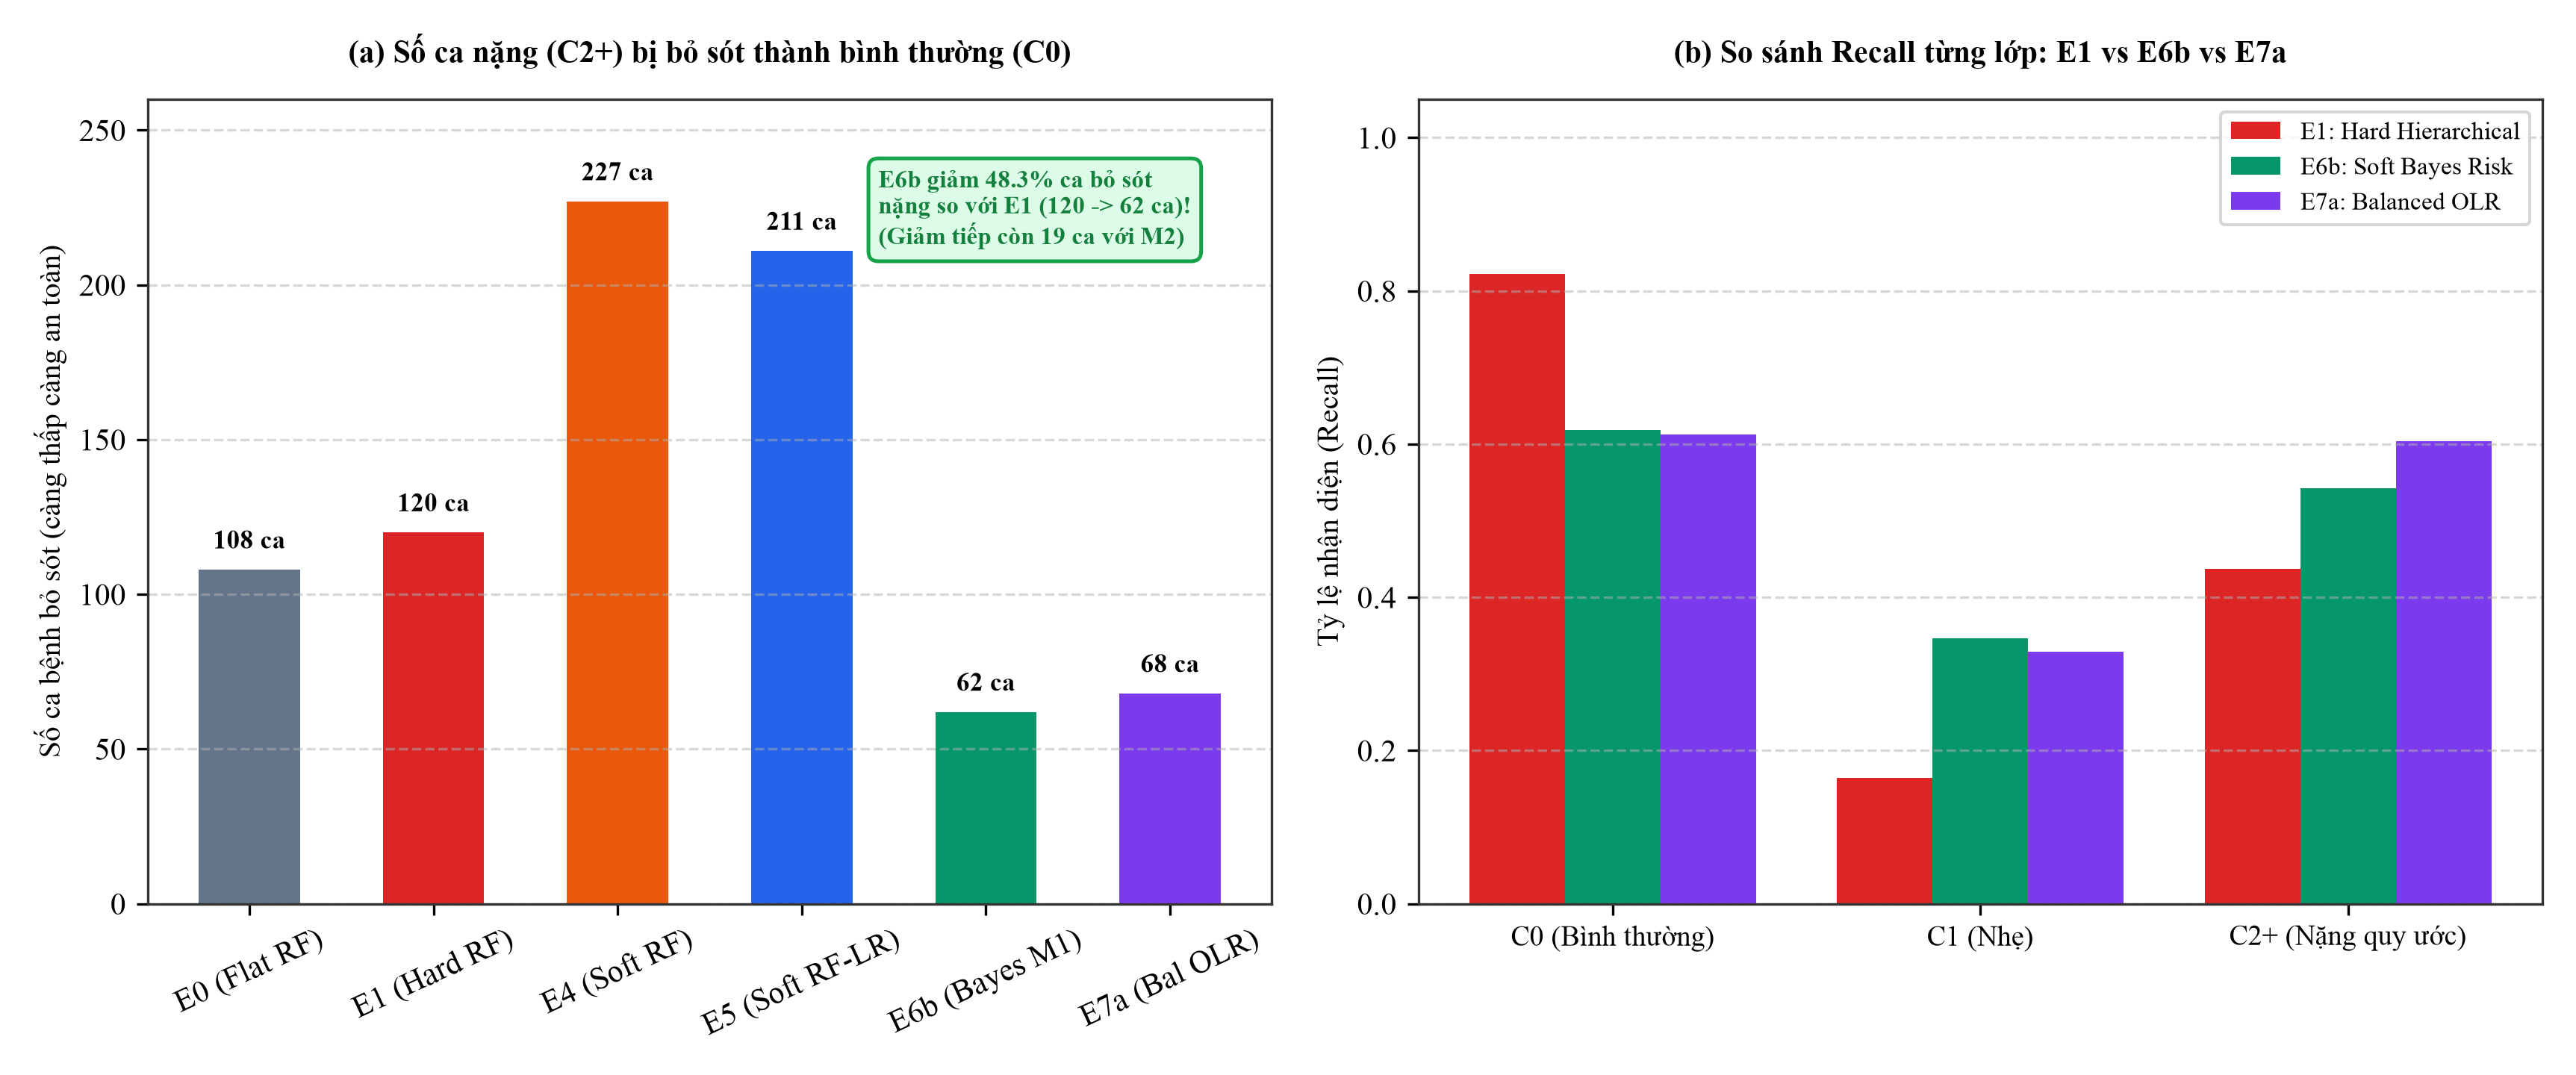
\includegraphics[width=\textwidth]{figures/fig4_confusion_error_analysis.png}
\label{fig:confusion-error-analysis}
\end{figure}
\FloatBarrier
\FloatBarrier

\subsection{Kết quả các mô hình phân loại thứ bậc ($E_7$)}
Bảng \ref{tab:ordinal-results} tổng hợp kết quả của các mô hình phân loại thứ bậc.

\begin{table}{Kết quả thực nghiệm các mô hình Ordinal Classification trên nhiệm vụ $T_3$ ($N = 4.045$)}
\centering
\footnotesize
\setlength{\tabcolsep}{3pt}
\label{tab:ordinal-results}
\begin{tabularx}{\textwidth}{l *{7}{>{\centering\arraybackslash}X}}
\toprule
\textbf{Mô hình} & \textbf{Macro-F1} & \textbf{BalAcc} & \textbf{Accuracy} & \textbf{Class MAE} & \textbf{QWK} & \textbf{Recall $C_1$} & \textbf{Recall $C_2^+$} \\
\midrule
$E_{7a}$ (OLR Unweighted) & 0.3846 & 0.4002 & \textbf{75.23\%} & \textbf{0.3377} & 0.2298 & 0.00\% & 22.00\% \\
$E_{7a}$ (OLR Balanced)   & \textbf{0.4518} & \textbf{0.5151} & 56.69\% & 0.5382 & 0.3398 & \textbf{32.93\%} & 60.37\% \\
$E_{7b}$ (CumBin LR)      & 0.3761 & 0.4949 & 63.41\% & 0.5718 & 0.2958 & 0.00\% & \textbf{72.88\%} \\
$E_{7b}$ (CumBin RF)      & 0.4191 & 0.4900 & 72.34\% & 0.3953 & \textbf{0.3744} & 0.16\% & 57.30\% \\
\bottomrule
\end{tabularx}
\end{table}


Mô hình Ordinal Logistic Regression cân bằng ($E_{7a}$ Balanced OLR) đạt \textbf{Balanced Accuracy cao nhất: 0.5151 $\pm$ 0.0152}, đồng thời nhận diện tương đối đồng đều trên cả 3 lớp: Recall $C_0 = 61.24\%$, Recall $C_1 = 32.93\%$ và Recall $C_2^+ = 60.37\%$ (Hình \ref{fig:confusion-error-analysis}b). Mặc dù Macro-F1 đạt 0.4518 (thấp hơn nhẹ so với $E_2$), sự cân bằng giữa các lớp của $E_{7a}$ tốt hơn.

Đối với mô hình Phân loại nhị phân tích lũy ($E_{7b}$ CumBin), do hai bộ phân loại $P(Y \ge 1)$ và $P(Y \ge 2)$ được huấn luyện độc lập, hiện tượng \textbf{vi phạm tính đơn điệu xác suất} $P(Y \ge 2) > P(Y \ge 1)$ xuất hiện trên thực tế (Hình \ref{fig:monotonicity-dist}): chiếm trung bình \textbf{19.53\%} tổng số dự đoán ngoài mẫu ở mô hình Logistic Regression ($E_{7b}$ CumBin LR) và \textbf{5.32\% $\pm$ 1.68\%} ở mô hình Random Forest ($E_{7b}$ CumBin RF). Sau khi áp dụng giải thuật hiệu chỉnh ngưỡng (Isotonic Probability Clipping), tỷ lệ vi phạm được đưa về 0.0\%. Tuy nhiên, việc ép xác suất $\tilde{P}(Y \ge 2) = \min(\hat{P}_1, \hat{P}_2)$ dẫn đến xác suất của lớp trung gian $P(C_1) = \hat{P}_1 - \tilde{P}_2$ bị gán bằng 0 tại các điểm vi phạm, khiến Recall của lớp $C_1$ bị suy giảm mạnh (Recall $C_1 = 0.00\%$ ở LR và $0.16\%$ ở RF).

\begin{figure}[htbp]{Phân bố vi phạm tính đơn điệu xác suất trong mô hình phân loại nhị phân tích lũy $E_{7b}$}
\centering
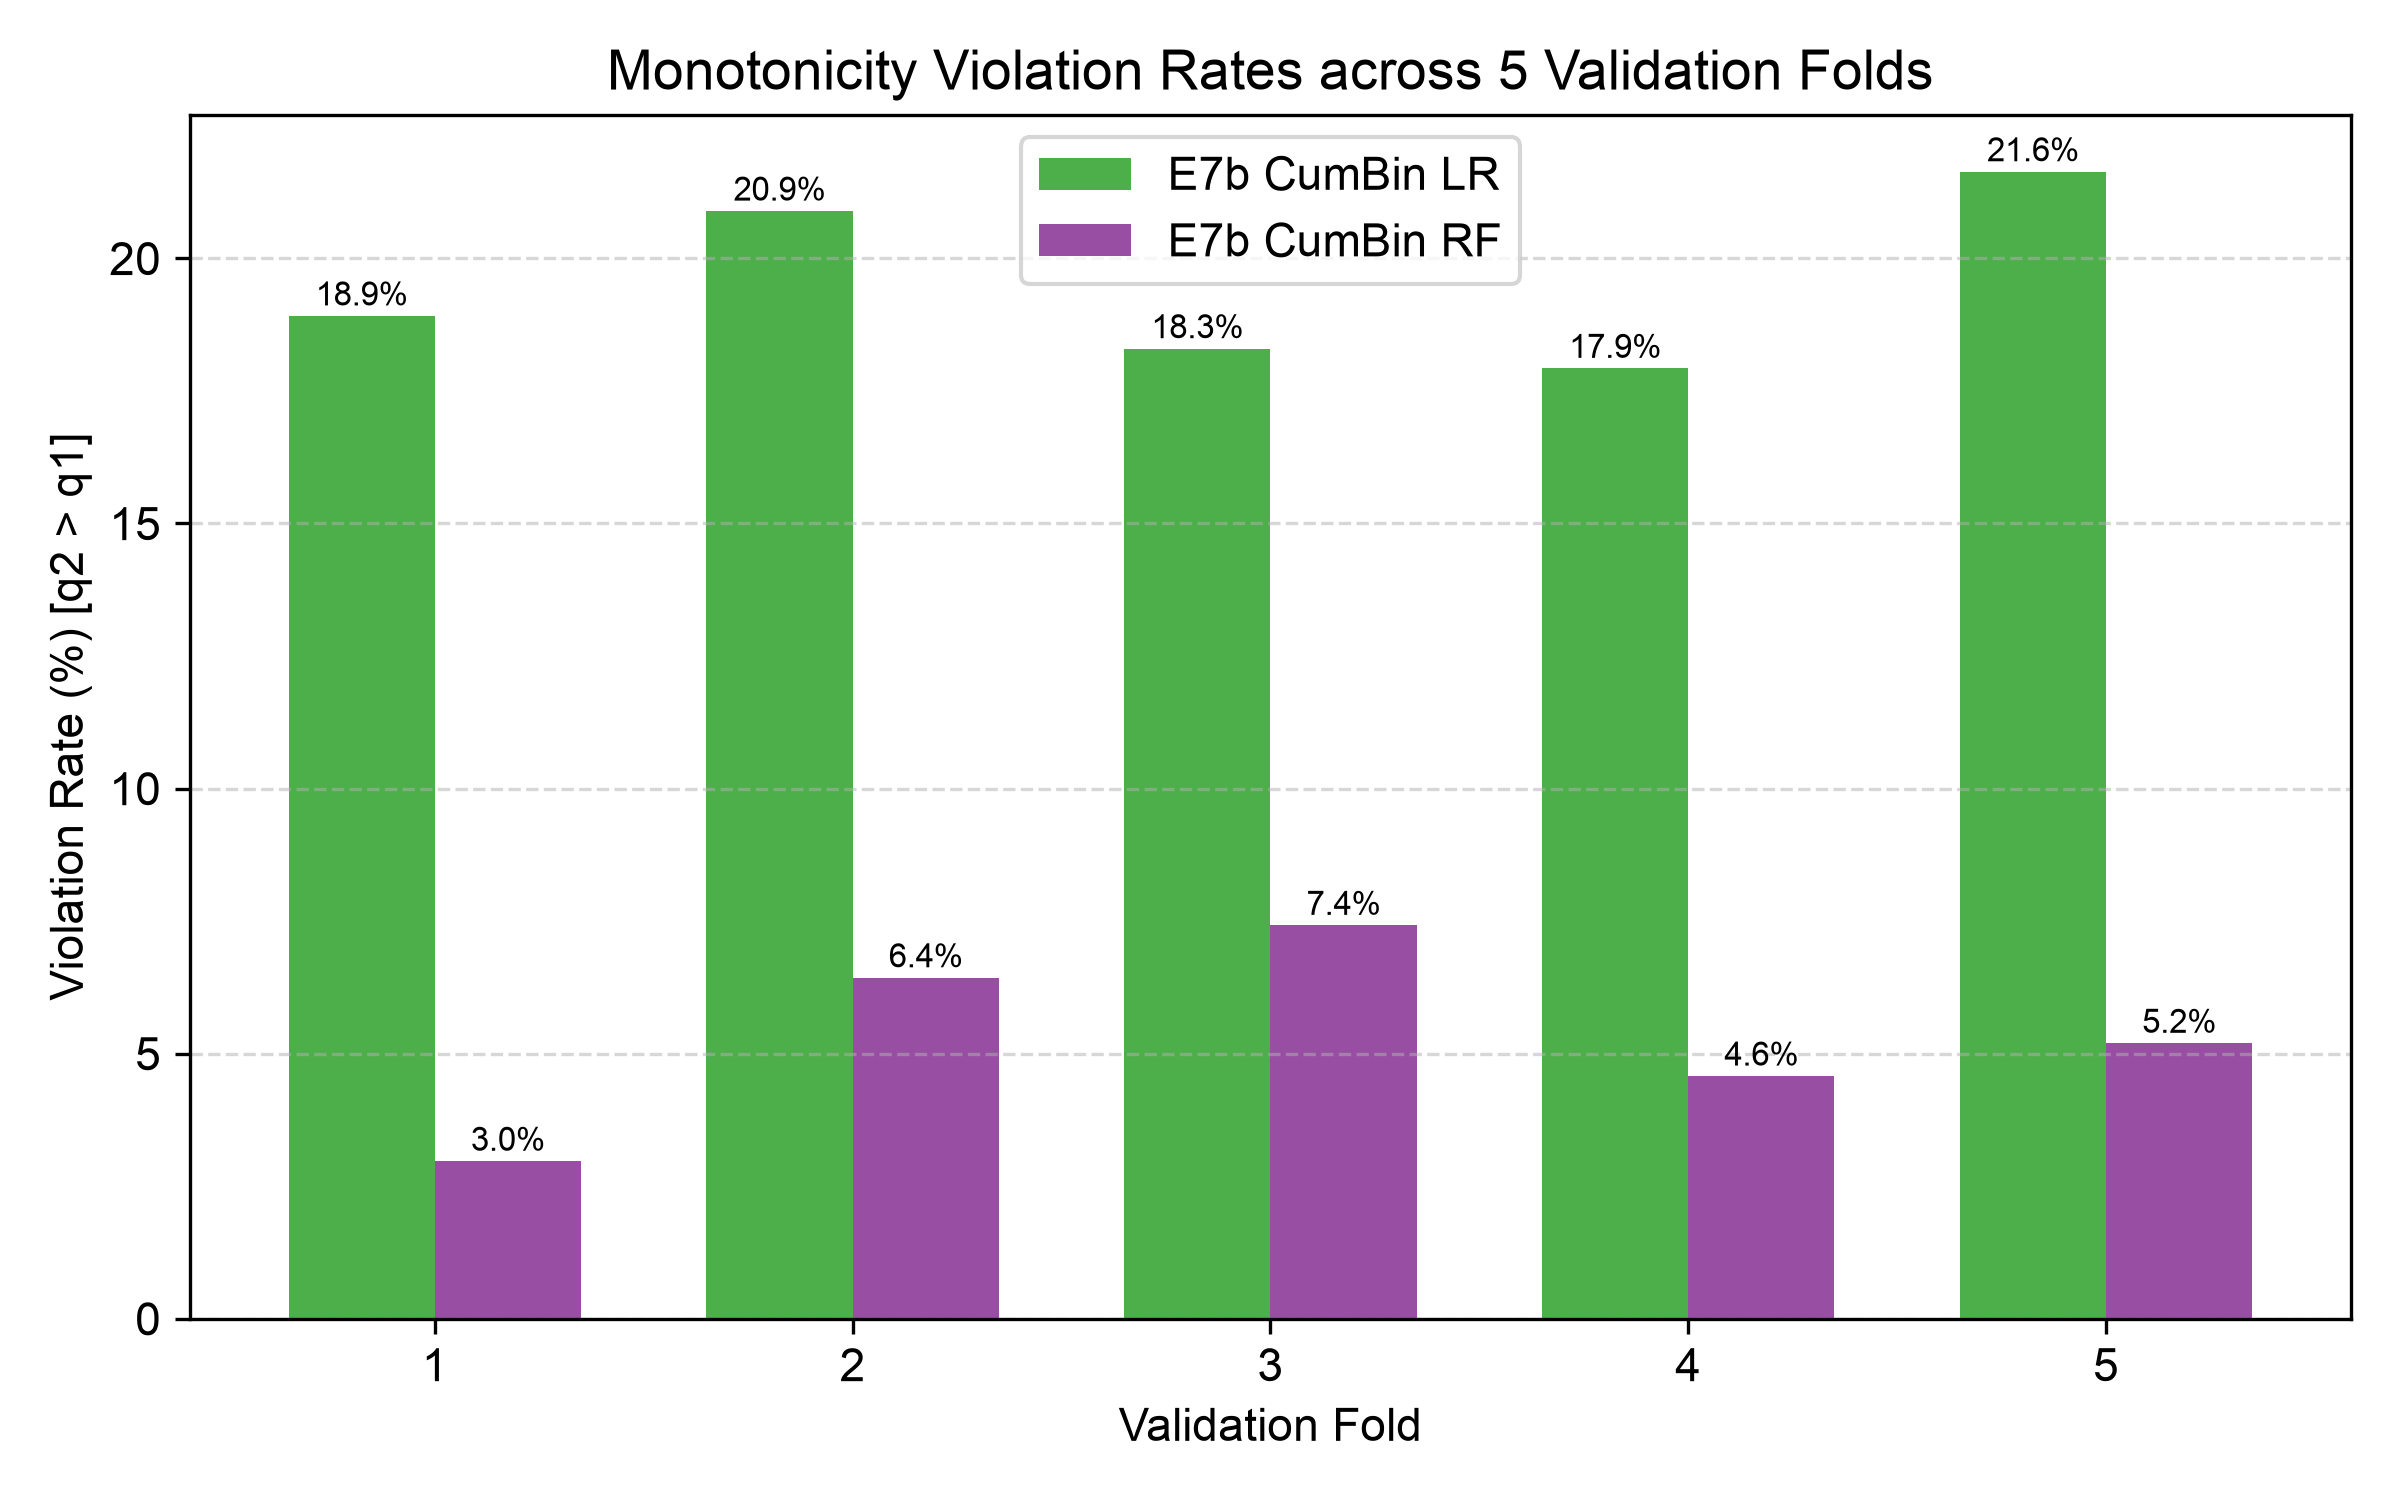
\includegraphics[width=0.8\textwidth]{figures/monotonicity_violation_distribution.png}
\label{fig:monotonicity-dist}
\end{figure}
\FloatBarrier

\subsection{Bảng so sánh tổng hợp các mô hình $T_3$}
Bảng \ref{tab:master-comparison} tổng hợp so sánh các mô hình từ $E_0$ đến $E_7$ trên hai nhóm chỉ số: hiệu năng phân loại tổng thể (Phần A) và các chỉ số liên quan đến sai số sàng lọc (Phần B).

\begin{table}{So sánh kết quả các mô hình trên nhiệm vụ $T_3$ ($N = 4.045$)}
\centering
\footnotesize
\setlength{\tabcolsep}{4pt}
\label{tab:master-comparison}

\vspace{-0.1cm}
\textbf{Phần A: Tổng hợp các chỉ số hiệu năng phân loại tổng thể}
\vspace{0.15cm}

\begin{tabularx}{\textwidth}{l X c c c c c}
\toprule
\textbf{Nhóm mô hình} & \textbf{Mô hình} & \textbf{Macro-F1} & \textbf{BalAcc} & \textbf{Accuracy} & \textbf{Class MAE} & \textbf{QWK} \\
\midrule
\textbf{Flat} & $E_0$ (Flat RF) & 0.4354 & 0.4667 & 64.10\% & 0.4638 & 0.3204 \\
\midrule
\multirow{4}{*}{\textbf{Hard Hier.}} 
  & $E_1$ (Hard RF--RF)   & 0.4550 & 0.4745 & 68.08\% & 0.4133 & 0.3705 \\
  & $E_2$ (Hard Tuned)    & \textbf{0.4586} & 0.4745 & 65.32\% & 0.4280 & 0.3644 \\
  & $E_{3a}$ (Hard RF--LR) & 0.4567 & 0.4964 & 68.43\% & 0.4195 & 0.3735 \\
  & $E_{3b}$ (Hard RF--XGB)& 0.4575 & 0.4790 & 68.23\% & 0.4180 & 0.3683 \\
\midrule
\multirow{2}{*}{\textbf{Soft Hier.}} 
  & $E_4$ (Soft RF--RF Argmax) & 0.4206 & 0.4309 & 73.75\% & 0.3530 & 0.3653 \\
  & $E_5$ (Soft RF--LR Argmax) & 0.4270 & 0.4506 & 73.37\% & 0.3619 & 0.3789 \\
\midrule
\multirow{2}{*}{\textbf{Cost-Sens.}}
  & $E_{6a}$ (Soft Cost RF--RF $M_1$) & 0.4535 & 0.4904 & 56.91\% & 0.5216 & 0.3235 \\
  & $E_{6b}$ (Soft Cost RF--LR $M_1$) & 0.4521 & 0.5025 & 56.84\% & 0.5197 & 0.3344 \\
\midrule
\multirow{4}{*}{\textbf{Ordinal}} 
  & $E_{7a}$ (OLR Unweighted) & 0.3846 & 0.4002 & \textbf{75.23\%} & \textbf{0.3377} & 0.2298 \\
  & $E_{7a}$ (OLR Balanced)   & 0.4518 & \textbf{0.5151} & 56.69\% & 0.5382 & 0.3398 \\
  & $E_{7b}$ (CumBin LR)      & 0.3761 & 0.4949 & 63.41\% & 0.5718 & 0.2958 \\
  & $E_{7b}$ (CumBin RF)      & 0.4191 & 0.4900 & 72.34\% & 0.3953 & \textbf{0.3744} \\
\midrule
\textbf{Baseline} & Majority Class ($C_0$) & 0.2848 & 0.3333 & 74.56\% & 0.3518 & 0.0000 \\
\bottomrule
\end{tabularx}

\vspace{0.35cm}
\textbf{Phần B: Khả năng nhận diện từng lớp và chỉ số sai số sàng lọc}
\vspace{0.15cm}

\begin{tabularx}{\textwidth}{l X c c c c c}
\toprule
\textbf{Nhóm mô hình} & \textbf{Mô hình} & \textbf{Recall $C_0$} & \textbf{Recall $C_1$} & \textbf{Recall $C_2^+$} & \textbf{$C_2^+ \to C_0$} & \textbf{$C_0 \to C_2^+$} \\
\midrule
\textbf{Flat} & $E_0$ (Flat RF) & 76.39\% & 16.29\% & 47.32\% & 108 ca & 316 ca \\
\midrule
\multirow{4}{*}{\textbf{Hard Hier.}} 
  & $E_1$ (Hard RF--RF)   & 82.16\% & 16.46\% & 43.74\% & 120 ca & 261 ca \\
  & $E_2$ (Hard Tuned)    & 77.02\% & 25.69\% & 39.63\% & 98 ca & 222 ca \\
  & $E_{3a}$ (Hard RF--LR) & 82.16\% & 11.75\% & 55.00\% & 120 ca & 300 ca \\
  & $E_{3b}$ (Hard RF--XGB)& 82.16\% & 16.77\% & 44.76\% & 120 ca & 279 ca \\
\midrule
\multirow{2}{*}{\textbf{Soft Hier.}} 
  & $E_4$ (Soft RF--RF Argmax) & 93.90\% & 5.18\% & 30.19\% & 227 ca & 139 ca \\
  & $E_5$ (Soft RF--LR Argmax) & 92.61\% & 3.45\% & 39.13\% & 211 ca & 176 ca \\
\midrule
\multirow{2}{*}{\textbf{Cost-Sens.}}
  & $E_{6a}$ (Soft Cost RF--RF $M_1$) & 61.94\% & \textbf{40.92\%} & 44.25\% & \textbf{62 ca} & 215 ca \\
  & $E_{6b}$ (Soft Cost RF--LR $M_1$) & 61.87\% & 34.64\% & 54.23\% & \textbf{62 ca} & 294 ca \\
\midrule
\multirow{4}{*}{\textbf{Ordinal}} 
  & $E_{7a}$ (OLR Unweighted) & 98.04\% & 0.00\% & 22.00\% & 305 ca & \textbf{59 ca} \\
  & $E_{7a}$ (OLR Balanced)   & 61.24\% & 32.93\% & 60.37\% & 68 ca & 357 ca \\
  & $E_{7b}$ (CumBin LR)      & 75.60\% & 0.00\% & \textbf{72.88\%} & 106 ca & 727 ca \\
  & $E_{7b}$ (CumBin RF)      & 89.56\% & 0.16\% & 57.30\% & 167 ca & 313 ca \\
\midrule
\textbf{Baseline} & Majority Class ($C_0$) & \textbf{100.00\%} & 0.00\% & 0.00\% & 391 ca & 0 ca \\
\bottomrule
\end{tabularx}

\vspace{0.15cm}
\raggedright
\scriptsize
\textit{Ghi chú:} Ký hiệu $M_1$ trong nhóm mô hình Cost-Sens. biểu thị việc áp dụng ma trận chi phí phạt lỗi Bayes $M_1$ ($\mathbf{C}(2, 0) = 3.0$). Các giá trị Recall là trung bình cộng qua 5 fold kiểm định chéo ngoài mẫu (đồng thời khớp tuyệt đối với tỷ lệ trên ma trận nhầm lẫn gộp pooled out-of-fold, độ lệch $< 0.02\%$). Số ca phân loại sai ($C_2^+ \to C_0$ và $C_0 \to C_2^+$) là số lượng tuyệt đối tổng hợp từ toàn bộ dự đoán ngoài mẫu (pooled OOF, $N = 4.045$).
\end{table}


Hình \ref{fig:legacy-comparison} trực quan hóa sự so sánh giữa các mô hình từ $E_0$ đến $E_6$. Hình \ref{fig:macro-vs-mae} và Hình \ref{fig:2step-errors} phân tích mối quan hệ giữa Macro-F1, Class MAE và tỷ lệ lỗi nhảy 2 bước ($C_2^+ \to C_0$).

\begin{figure}[htbp]{So sánh trực quan hiệu năng giữa các mô hình từ $E_0$ đến $E_6$ trên tập Legacy}
\centering
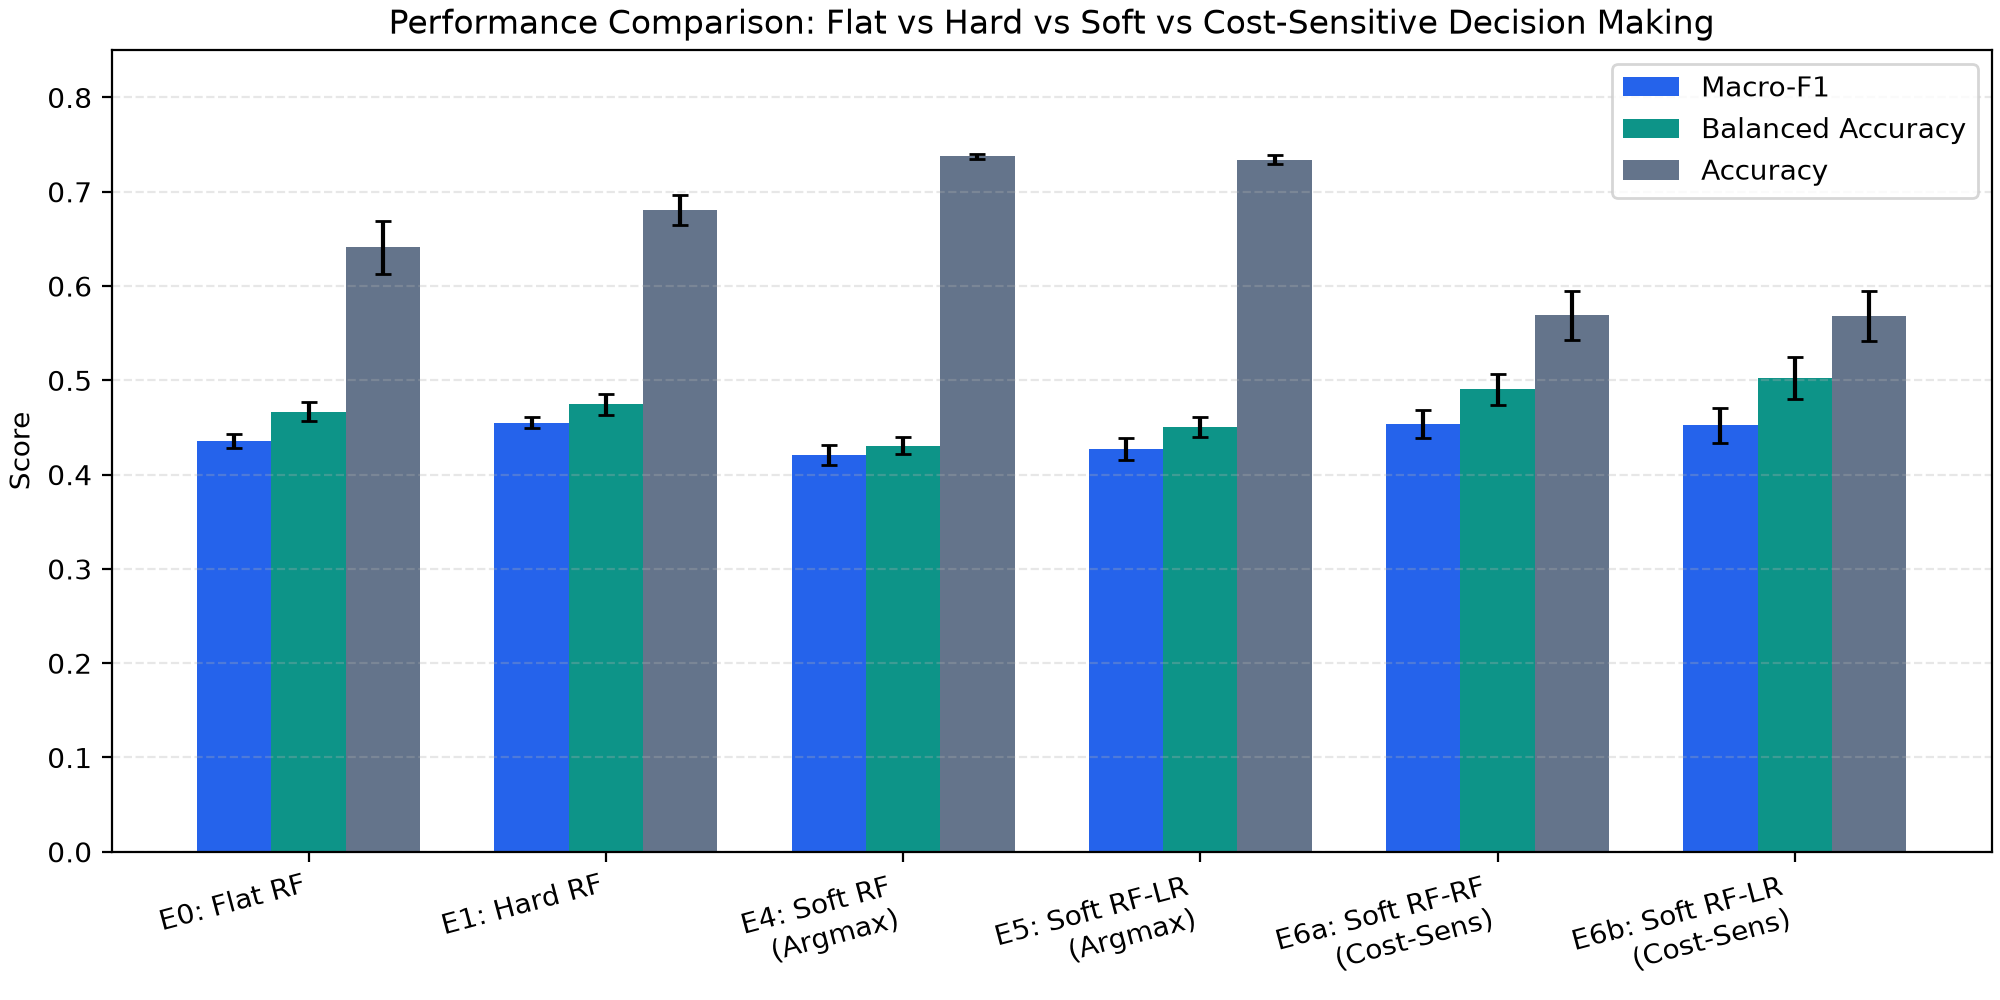
\includegraphics[width=0.85\textwidth]{figures/legacy_model_comparison_e0_to_e6.png}
\label{fig:legacy-comparison}
\end{figure}
\FloatBarrier

\begin{figure}[htbp]{Mối quan hệ đánh đổi giữa Macro-F1 và Class MAE giữa các hướng tiếp cận mô hình}
\centering
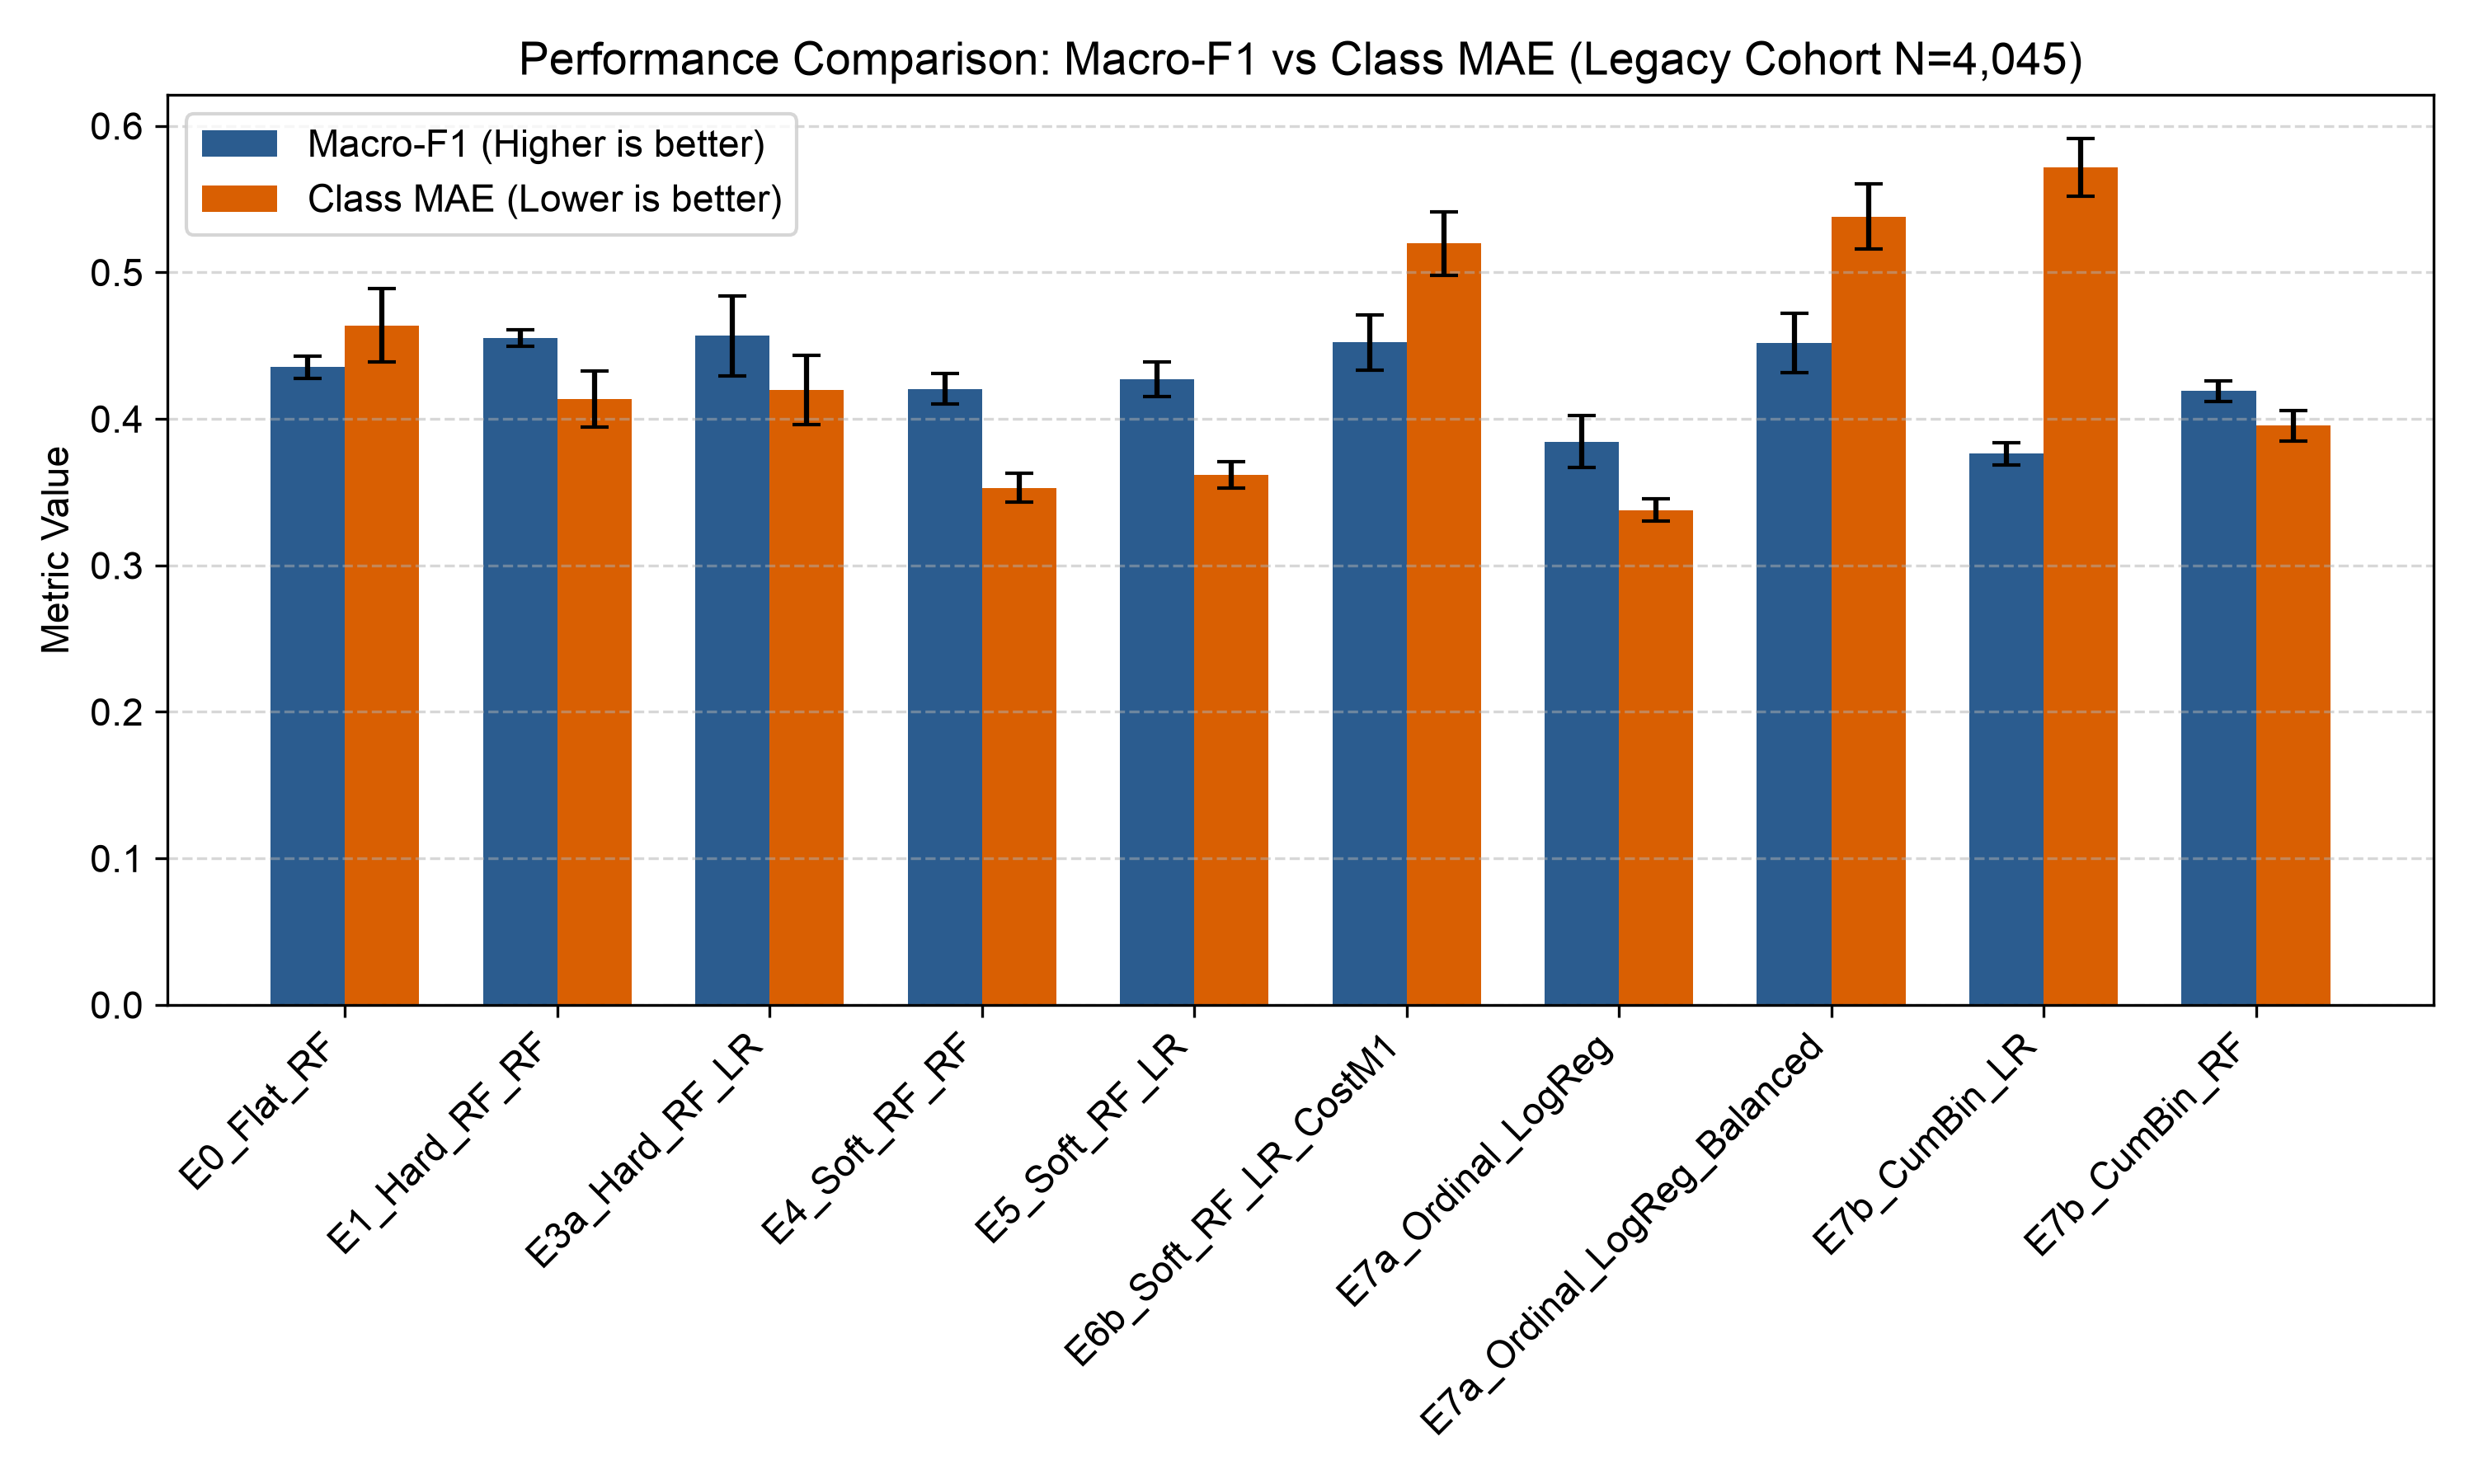
\includegraphics[width=0.85\textwidth]{figures/macro_f1_vs_mae.png}
\label{fig:macro-vs-mae}
\end{figure}
\FloatBarrier

\begin{figure}[htbp]{So sánh số lượng lỗi nhảy 2 bước ($C_2^+ \to C_0$) giữa các mô hình}
\centering
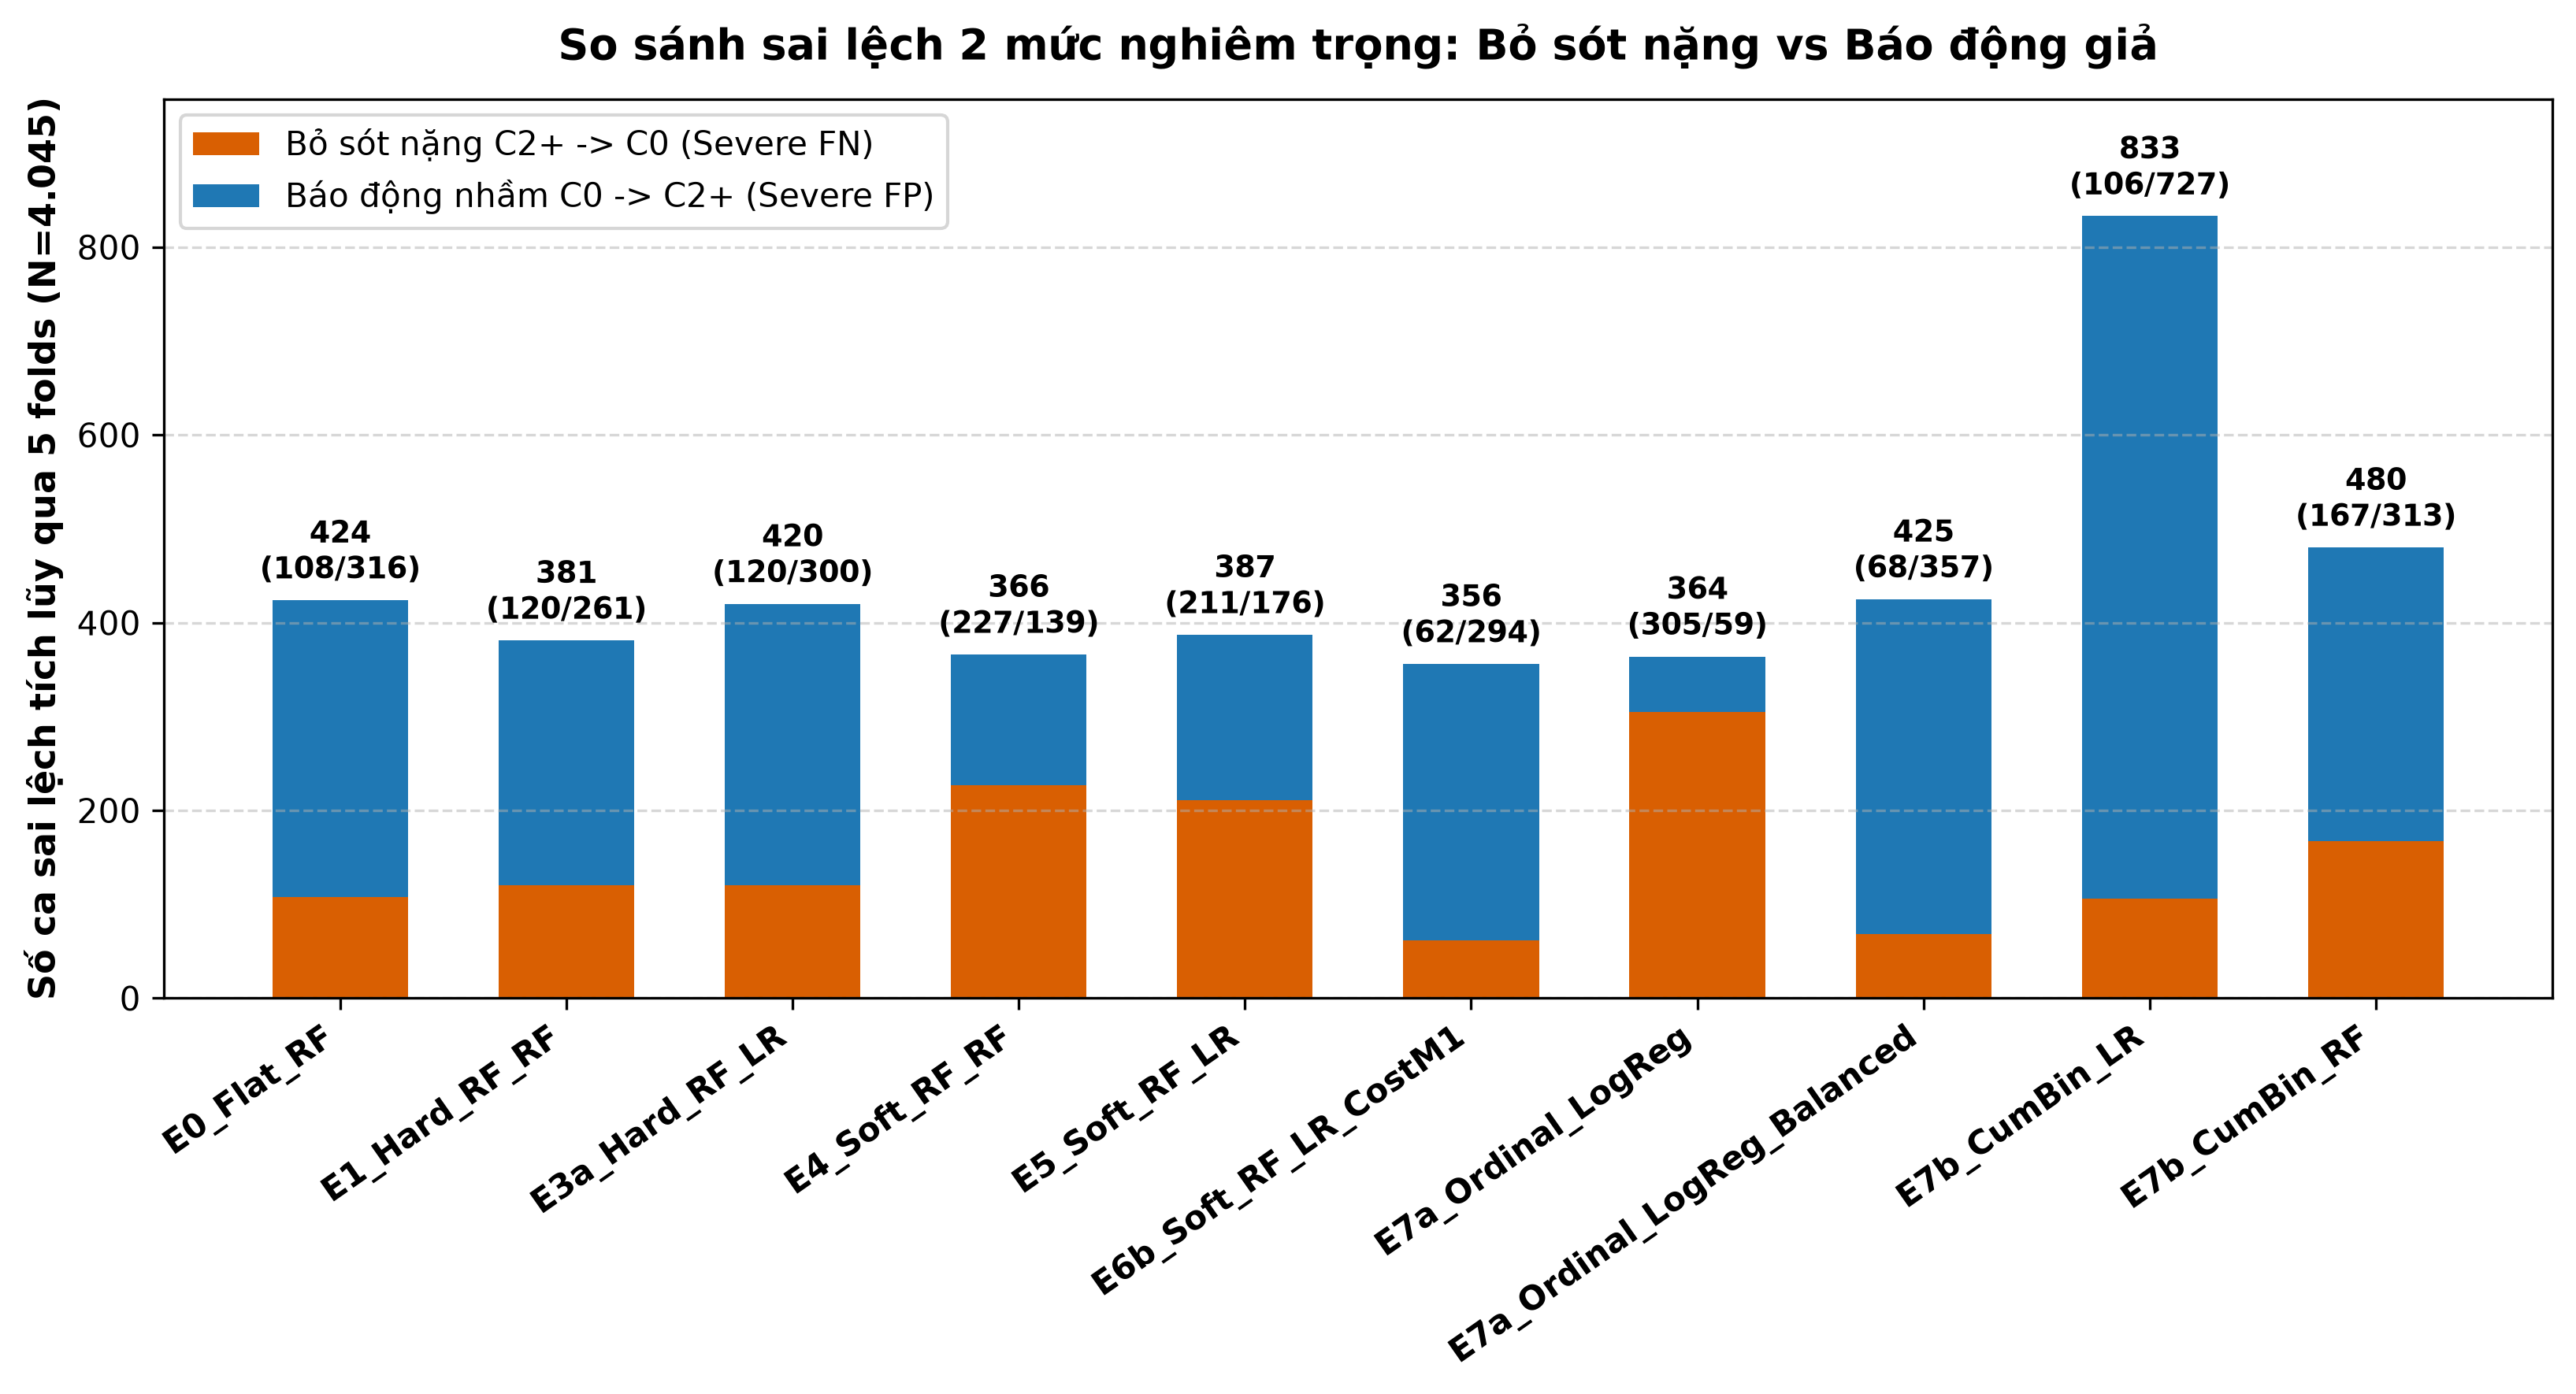
\includegraphics[width=0.85\textwidth]{figures/2step_error_comparison.png}
\label{fig:2step-errors}
\end{figure}
\FloatBarrier

Hình \ref{fig:conf-p1} và Hình \ref{fig:conf-p2} trình bày ma trận nhầm lẫn chi tiết của 6 mô hình đại diện: $E_0, E_1, E_5, E_{6b}, E_{7a}, E_{7b}$.

\begin{figure}[htbp]{Ma trận nhầm lẫn của 4 mô hình đại diện: $E_0$ (Flat RF), $E_1$ (Hard RF--RF), $E_5$ (Soft RF--LR) và $E_{6b}$ (Cost-Sensitive)}
\centering
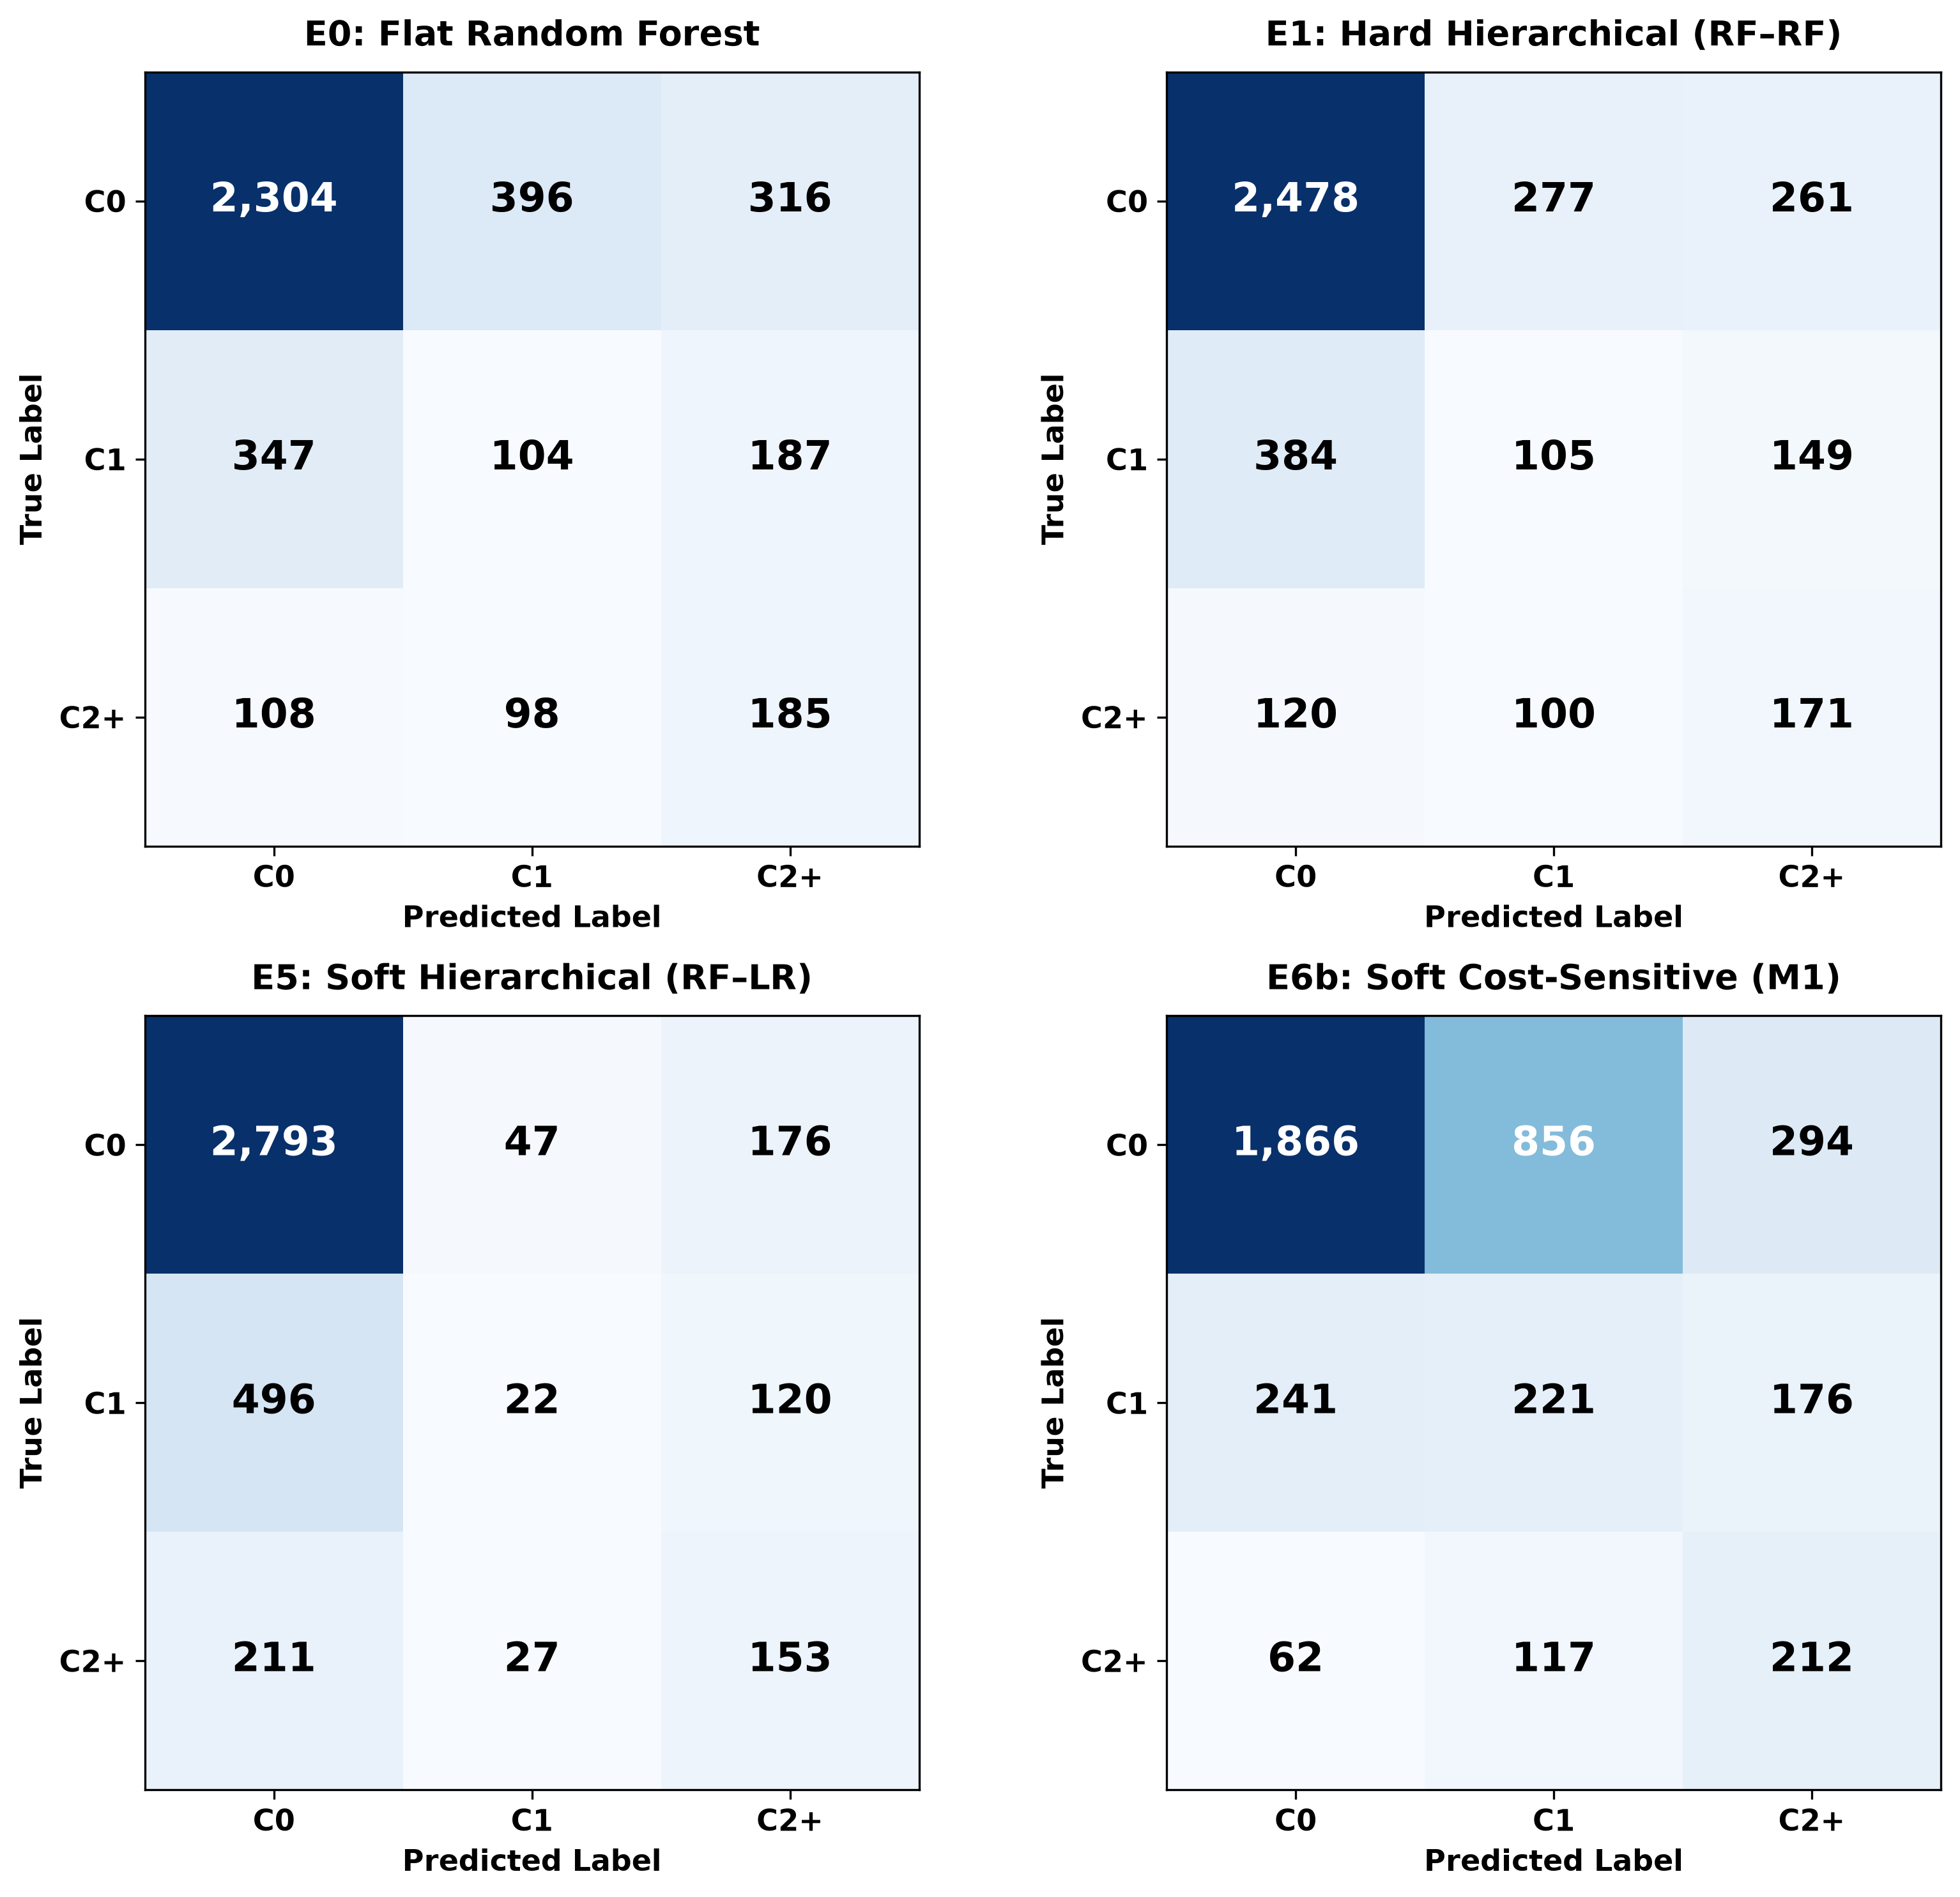
\includegraphics[width=0.95\textwidth]{figures/confusion_matrices_group1.png}
\label{fig:conf-p1}
\end{figure}
\FloatBarrier

\begin{figure}[htbp]{Ma trận nhầm lẫn của 2 mô hình phân loại thứ bậc: $E_{7a}$ (Balanced OLR) và $E_{7b}$ (CumBin RF)}
\centering
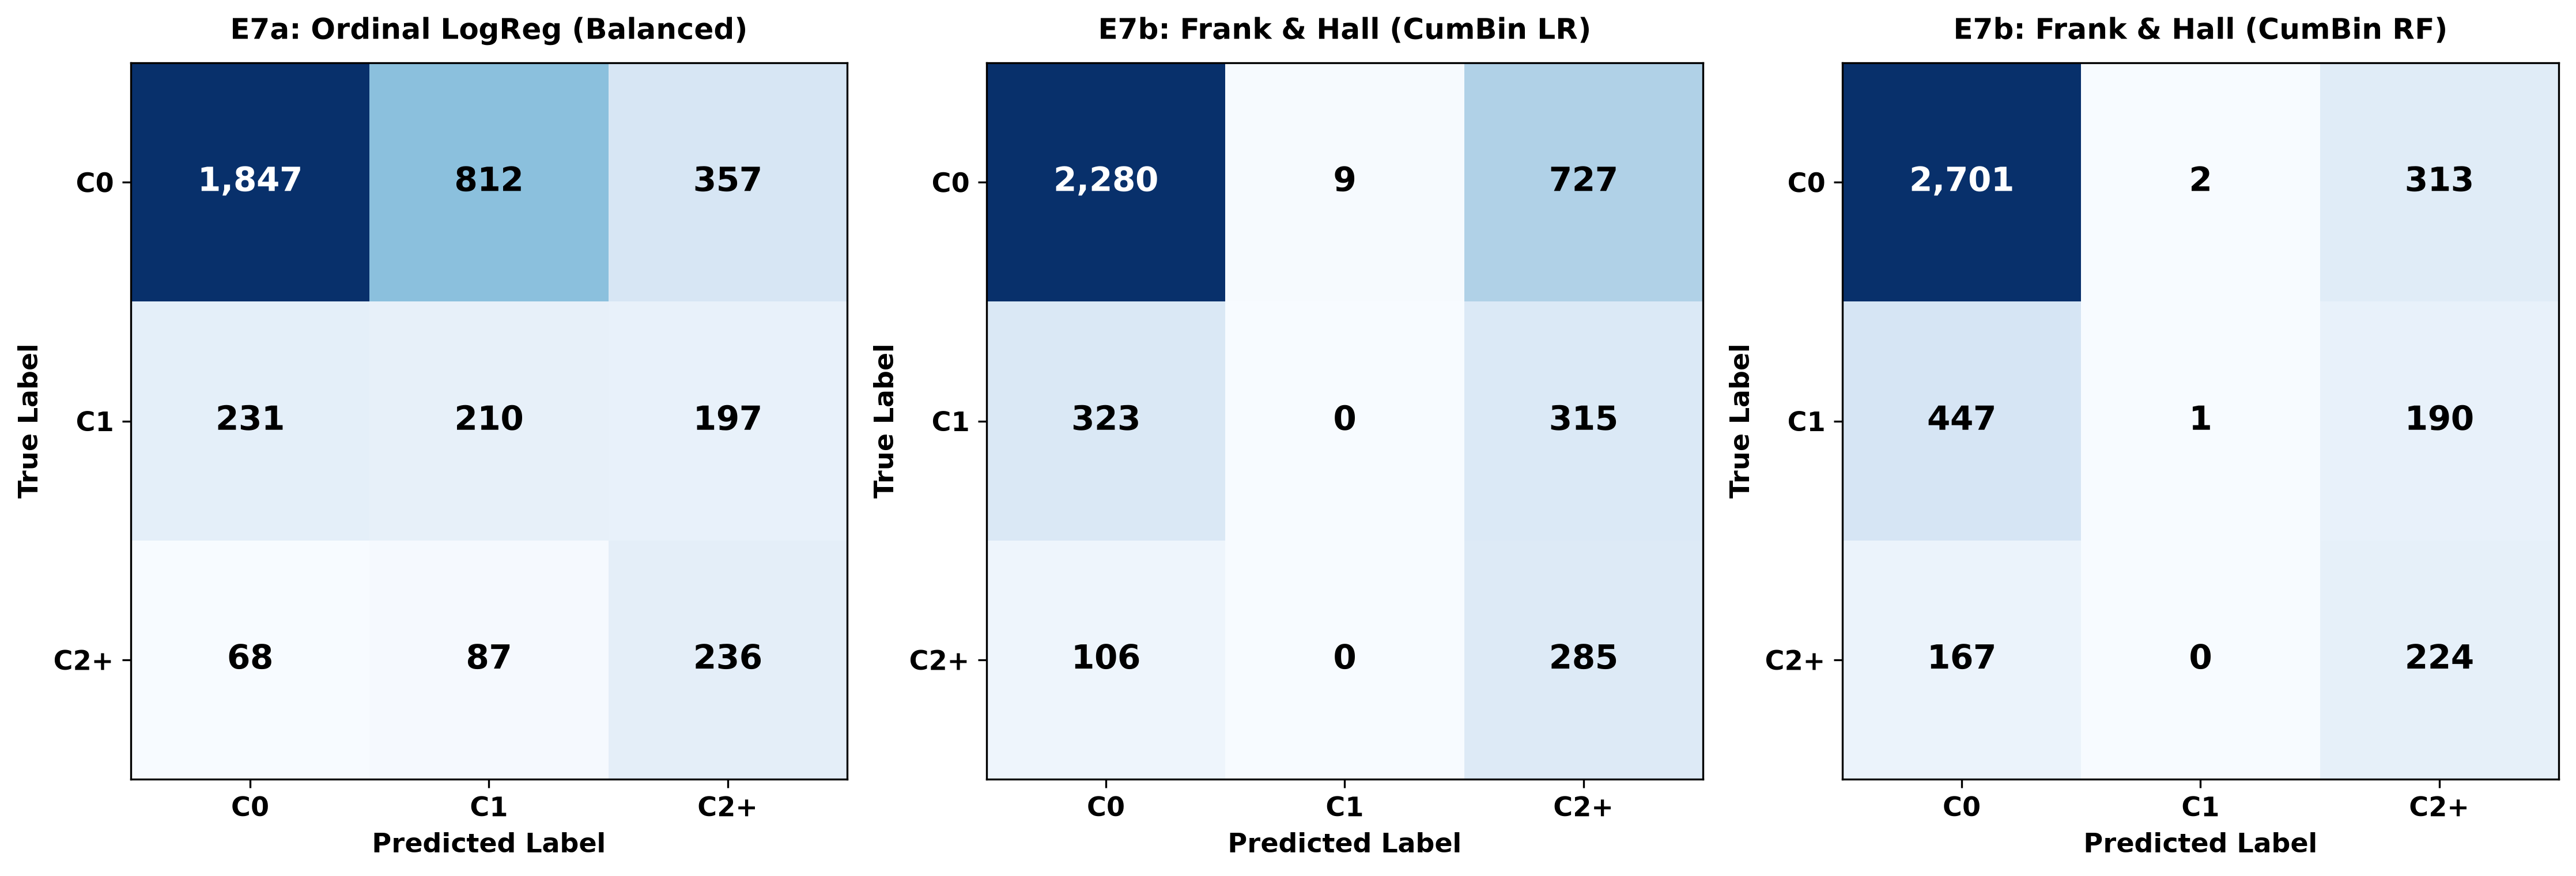
\includegraphics[width=0.95\textwidth]{figures/confusion_matrices_group2.png}
\label{fig:conf-p2}
\end{figure}
\FloatBarrier

\section{Phân tích sự đánh đổi sai số và ma trận chi phí}
\label{sec:danh-doi-lam-sang}

Một kết quả thực nghiệm quan trọng của DepSev-ML là định lượng sự đánh đổi giữa hai loại sai số (Hình \ref{fig:cost-tradeoff}):
\begin{itemize}
    \item \textbf{Sai số bỏ sót ca nặng ($C_2^+ \to C_0$):} Nguy cơ bỏ sót đối tượng có triệu chứng nặng trong quá trình sàng lọc.
    \item \textbf{Sai số báo động nhầm ($C_0 \to C_2^+$):} Khiến đối tượng có triệu chứng tối thiểu bị phân loại nhầm vào nhóm nặng, làm tăng chi phí theo dõi không cần thiết.
\end{itemize}

\begin{figure}[htbp]{Đường cong đánh đổi giữa tỷ lệ nhận diện ca nặng ($C_2^+$ Recall) và tỷ lệ báo động nhầm ($C_0$ False Alarm Rate)}
\centering
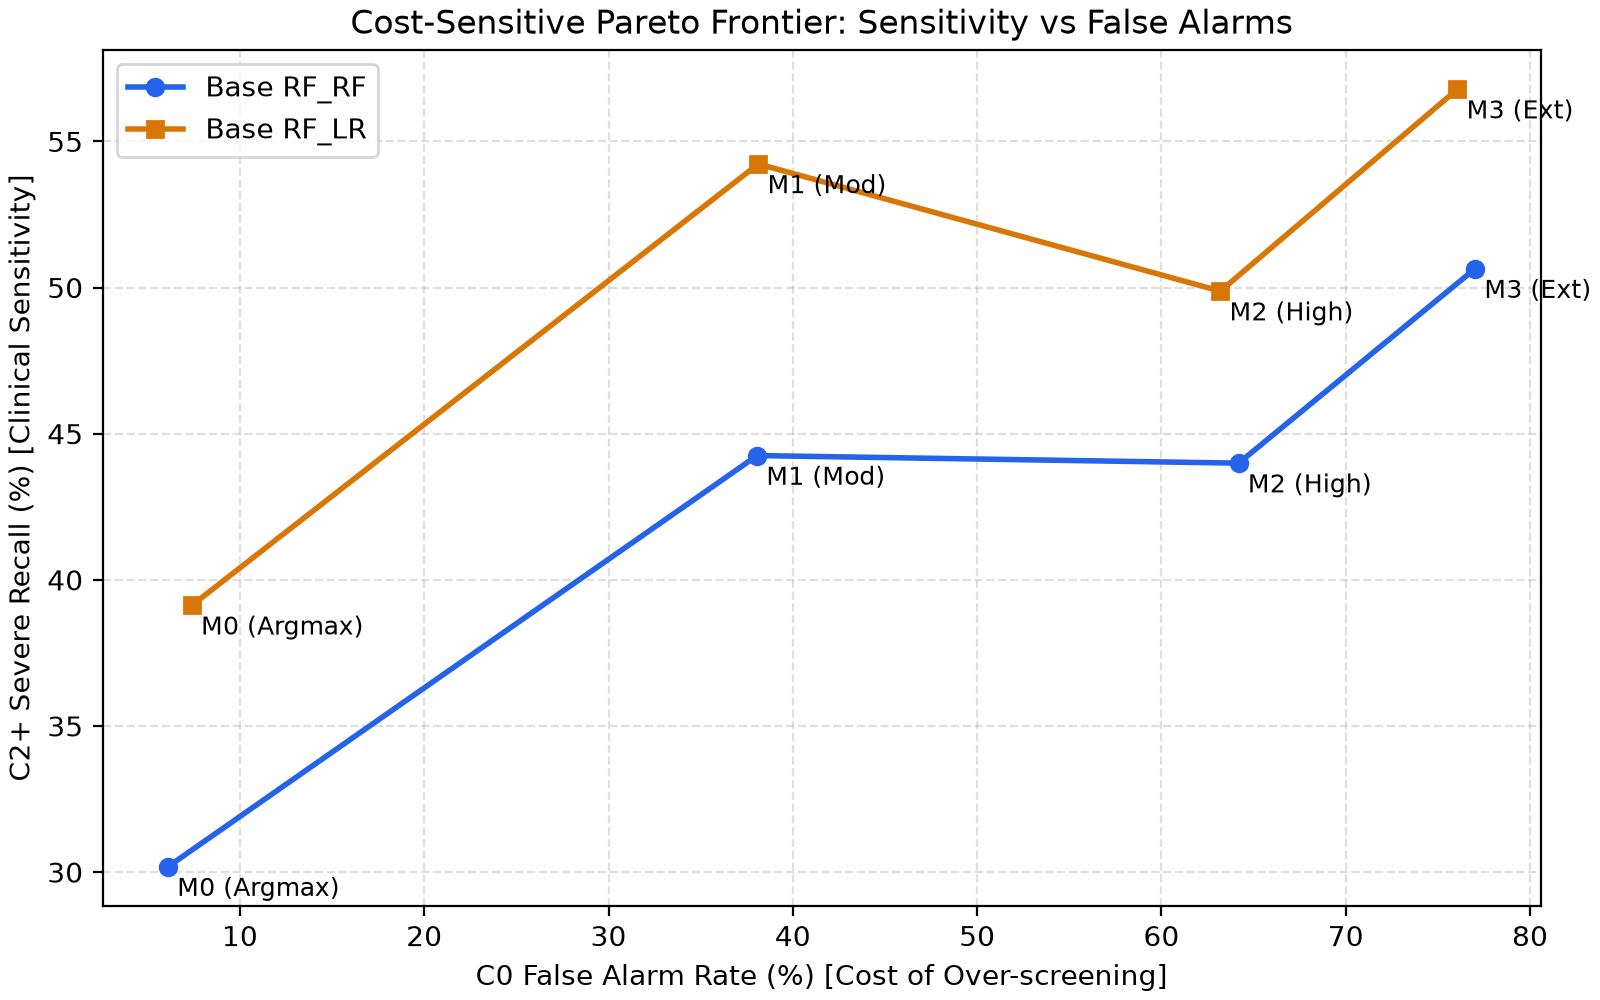
\includegraphics[width=0.85\textwidth]{figures/cost_tradeoff_curve.png}
\label{fig:cost-tradeoff}
\end{figure}
\FloatBarrier

Khi điều chỉnh mức độ phạt từ ma trận $M_0$ (chi phí đồng nhất) đến $M_3$ (phạt tối đa lỗi bỏ sót ca nặng $\mathbf{C}(2, 0) = 8.0$):
\begin{itemize}
    \item Số ca nặng bị bỏ sót thành bình thường ($C_2^+ \to C_0$) giảm từ \textbf{120 ca ($E_1$)} xuống còn \textbf{62 ca ($E_{6b}$, ma trận $M_1$)}, tương đương mức giảm \textbf{48.33\%} (tỷ lệ bỏ sót giảm từ 30.69\% xuống 15.86\%). Khi tăng cường mức phạt sang $M_2$ ($\mathbf{C}(2, 0) = 5.0$) và $M_3$ ($\mathbf{C}(2, 0) = 8.0$), số ca bỏ sót tiếp tục giảm xuống lần lượt \textbf{19 ca} (giảm 84.17\%) và \textbf{7 ca} (giảm 94.17\%). (Lưu ý: ở cấu hình phân cấp mềm $E_5$ sử dụng hàm argmax thuần túy, do xu hướng thiên lệch về lớp đa số $C_0$, số ca bỏ sót là 211 ca).
    \item Đổi lại, số ca bình thường bị xếp sang nhóm có triệu chứng ($C_0 \to \{C_1, C_2^+\}$) tăng từ 538 ca ($E_1$) lên \textbf{1.150 ca ($E_{6b}$, $M_1$)} (trong đó 294 ca bị xếp trực tiếp thành $C_2^+$), và tiếp tục tăng lên 1.906 ca ($M_2$) cùng 2.294 ca ($M_3$).
\end{itemize}
Đây là quy luật đánh đổi tự nhiên trong sàng lọc sức khỏe cộng đồng. Khung làm việc DepSev-ML cho phép lựa chọn ma trận chi phí phù hợp tùy thuộc vào năng lực tiếp nhận của hệ thống y tế thực tế.

\section{Kiểm định ngoại suy theo dòng thời gian (Temporal Validation)}
\label{sec:temporal-results}

Để kiểm tra xem liệu các kết quả trên có bị quá khớp trên một chu kỳ khảo sát đơn lẻ hay không, nghiên cứu thực hiện kiểm định ngoại suy trên tập dữ liệu độc lập NHANES 2015--2016 ($N = 4.888$, Branch D). Toàn bộ các mô hình được huấn luyện trên dữ liệu gộp hai chu kỳ 2011--2014 ($N = 9.693$) và kiểm định ngoại suy một lần duy nhất trên chu kỳ 2015--2016 ($N = 4.888$), áp dụng trên không gian 31 đặc trưng hài hòa hóa ($F_{4\_\text{common31}}$).

Kết quả được trình bày trong Bảng \ref{tab:multicycle-temporal-results}. Hình \ref{fig:multicycle-soft-temporal} minh họa sự so sánh hiệu năng của các mô hình phân cấp mềm và nhạy chi phí qua ba nhánh dữ liệu (Branch A, B, D).

\begin{table}{Kết quả kiểm định ngoại suy theo dòng thời gian (Branch D, NHANES 2015--2016, $N = 4.888$)}
\centering
\footnotesize
\setlength{\tabcolsep}{3pt}
\label{tab:multicycle-temporal-results}
\begin{tabularx}{\textwidth}{l *{7}{>{\centering\arraybackslash}X}}
\toprule
\textbf{Mô hình ($T_3$)} & \textbf{Macro-F1} & \textbf{BalAcc} & \textbf{Accuracy} & \textbf{Recall $C_0$} & \textbf{Recall $C_1$} & \textbf{Recall $C_2^+$} & \textbf{Class MAE} \\
\midrule
$E_0$ (Flat RF)                     & 0.4345 & 0.4908 & 62.68\% & 73.66\% & 18.79\% & 54.77\% & 0.5008 \\
$E_1$ (Hard RF--RF)                 & \textbf{0.4393} & 0.4879 & 66.35\% & 79.86\% & 14.51\% & 52.01\% & 0.4556 \\
$E_4$ (Soft RF--RF)                 & 0.4223 & 0.4594 & \textbf{71.91\%} & 90.60\% & 4.76\% & 42.46\% & \textbf{0.3766} \\
$E_5$ (Soft RF--LR)                 & 0.4265 & 0.4681 & 71.79\% & 90.08\% & 4.88\% & 45.48\% & 0.3801 \\
$E_{6b}$ (Soft Cost $M_2$)          & 0.3439 & 0.4691 & 34.84\% & 26.94\% & \textbf{60.29\%} & 53.52\% & 0.7306 \\
$E_{7a}$ (OLR Balanced)             & 0.4349 & \textbf{0.5073} & 56.28\% & 61.74\% & 31.15\% & 59.30\% & 0.5503 \\
$E_{7b}$ (CumBin LR)                & 0.3632 & 0.4982 & 62.21\% & 75.23\% & 0.12\% & \textbf{74.12\%} & 0.5833 \\
$E_{7b}$ (CumBin RF)                & 0.3861 & 0.4861 & 67.88\% & 84.16\% & 0.36\% & 61.31\% & 0.4695 \\
\bottomrule
\end{tabularx}

\vspace{0.15cm}
\raggedright
\scriptsize
\textit{Ghi chú:} Mô hình được huấn luyện trên dữ liệu 2 chu kỳ 2011--2014 ($N = 9.693$) và kiểm tra ngoại suy độc lập một lần duy nhất trên chu kỳ 2015--2016 ($N = 4.888$) với không gian 31 đặc trưng hài hòa ($F_{4\_\text{common31}}$). Cấu hình $E_{6b}$ ở đây áp dụng ma trận chi phí phạt nặng $M_2$, dẫn đến Recall $C_0$ giảm còn 26.94\% để ưu tiên độ nhạy cho các nhóm có triệu chứng.
\end{table}


\begin{figure}[htbp]{So sánh hiệu năng các mô hình phân cấp mềm và nhạy chi phí giữa chu kỳ đơn lẻ (Branch A), gộp đa chu kỳ (Branch B) và kiểm định thời gian (Branch D)}
\centering
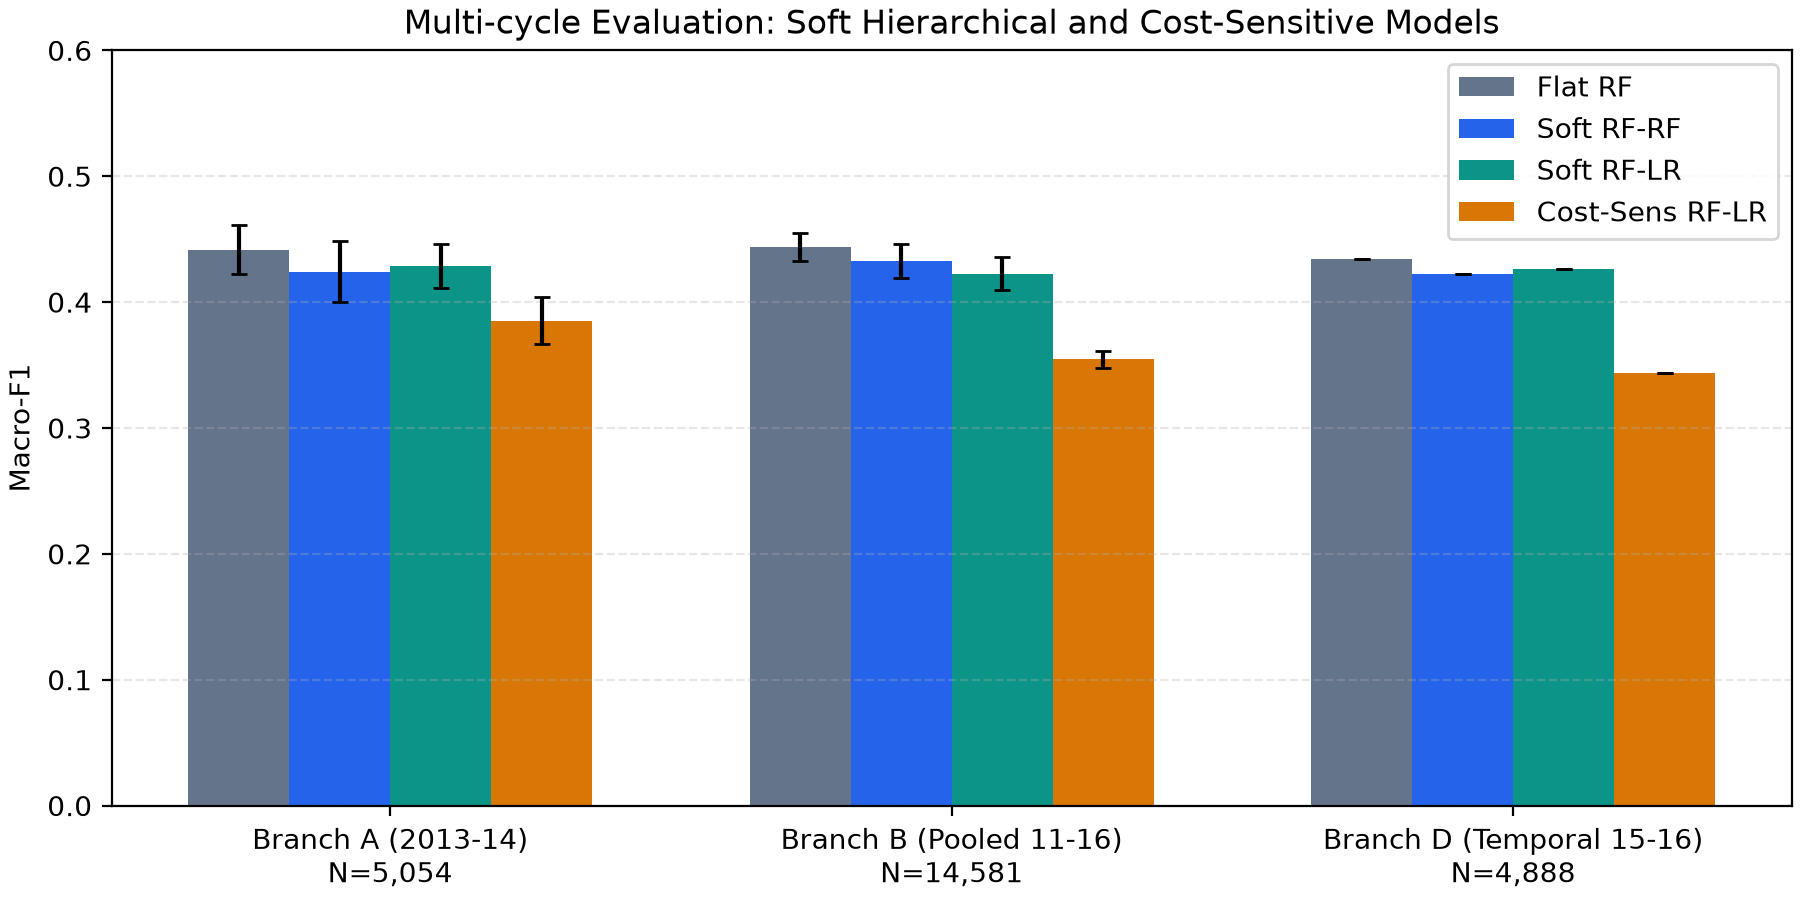
\includegraphics[width=0.85\textwidth]{figures/multicycle_soft_comparison.png}
\label{fig:multicycle-soft-temporal}
\end{figure}
\FloatBarrier

Một số phát hiện từ kiểm định dòng thời gian:
\begin{enumerate}
    \item \textbf{Độ ổn định của Balanced OLR ($E_{7a}$):} Mô hình Ordinal Logistic Regression cân bằng đạt Balanced Accuracy = \textbf{0.5073} trên tập dữ liệu tương lai (so với 0.5151 ở kiểm định chéo nội chu kỳ), mức suy giảm chỉ 1.5\%. Khả năng nhận diện ca nặng Recall $C_2^+$ đạt 59.30\%, cho thấy tính ổn định của cấu trúc siêu phẳng ranh giới song song trước hiện tượng dịch chuyển phân phối dữ liệu theo thời gian.
    \item \textbf{Đặc điểm của các mô hình phân cấp mềm và hàm phạt cao:} Các mô hình phân cấp mềm và mô hình áp dụng ma trận chi phí phạt cao ($E_{6b}$ với $M_2$) có sự sụt giảm độ chính xác tổng thể do dịch chuyển ngưỡng xác suất ngoài mẫu, cho thấy các mô hình tuyến tính có cấu trúc thứ bậc như OLR duy trì độ ổn định ngoại suy tốt hơn trên dữ liệu cộng đồng.
\end{enumerate}

\section{Thảo luận tổng hợp các phát hiện chính}
\label{sec:thao-luan-tong-hop}

Mặc dù nghiên cứu đã khảo sát 8 mô hình ($E_0 \to E_7$) nhằm đánh giá có hệ thống các hướng tiếp cận, các phát hiện thực nghiệm chính có thể được tóm lược qua \textbf{bốn mô hình tiêu biểu đại diện cho 4 tiêu chí cốt lõi} trong Bảng \ref{tab:executive-decision-matrix}.

\begin{table}{Tổng hợp các mô hình tiêu biểu theo từng tiêu chí}
\centering
\footnotesize
\setlength{\tabcolsep}{4pt}
\label{tab:executive-decision-matrix}
\begin{tabularx}{\textwidth}{p{3.2cm} p{3.0cm} p{3.2cm} X}
\toprule
\textbf{Tiêu chí xem xét} & \textbf{Mô hình tiêu biểu} & \textbf{Kết quả đạt được} & \textbf{Ý nghĩa thực tiễn và Đánh giá} \\
\midrule
\textbf{Phân loại 5 mức ($T_5$)} & \textbf{Random Forest (Tuned)} & Macro-F1 = 0.2755 \newline Weighted-F1 = 0.6437 & Mô hình cơ sở tốt nhất trên không gian phẳng gốc; phản ánh giới hạn phân tách của tập đặc trưng sinh lý ngoại vi. \\
\midrule
\textbf{Macro-F1 cao nhất trên $T_3$} & \textbf{$E_2$ (Hard RF--RF Tuned)} & Macro-F1 = \textbf{0.4586} \newline BalAcc = 0.4745 & Đạt điểm Macro-F1 cao nhất nhưng có nguy cơ bỏ sót 98 ca nặng ($C_2^+$) thành bình thường ($C_0$) do sai số một chiều ở Stage 1. \\
\midrule
\textbf{Cân bằng giữa các lớp} & \textbf{$E_{7a}$ (Balanced OLR)} & BalAcc = \textbf{0.5151} \newline Temporal BalAcc = \textbf{0.5073} & Phân bổ độ nhạy tương đối đồng đều trên cả 3 nhóm triệu chứng và duy trì độ ổn định tốt qua kiểm định ngoại suy theo thời gian. \\
\midrule
\textbf{Giảm bỏ sót ca nặng} & \textbf{$E_{6b}$ (Soft Bayes Risk, $M_1$)} & Bỏ sót $C_2^+$ còn \textbf{62 ca} \newline (giảm \textbf{48.3\%} so với $E_1$), BalAcc = 0.5025 & Thích hợp cho mục tiêu sàng lọc y tế dự phòng; giảm số ca nặng bị bỏ sót thành bình thường từ 120 ca ($E_1$) xuống 62 ca (và 19 ca với $M_2$). \\
\bottomrule
\end{tabularx}
\end{table}


Ý nghĩa và vai trò của từng mô hình tiêu biểu:
\begin{enumerate}
    \item \textbf{Random Forest Tuned (Mô hình đối chuẩn trên $T_5$):} Là mô hình học máy cơ sở phù hợp nhất trên không gian phẳng 5 lớp gốc, đạt Macro-F1 = $0.2755 \pm 0.0270$ và Weighted-F1 = $0.6437 \pm 0.0087$. Mô hình này xác lập mốc đối chuẩn và phản ánh rõ nét đặc tính phân tách của các đặc trưng sinh lý ngoại vi dạng bảng.
    \item \textbf{$E_2$ Hard RF--RF Tuned (Tối ưu Macro-F1 trên $T_3$):} Đạt Macro-F1 cao nhất trong các mô hình $T_3$ được khảo sát (\textbf{0.4586}), cải thiện so với mô hình phẳng $E_0$ (0.4354). Tuy nhiên, mô hình thể hiện đặc điểm sai số một chiều khi có 98 ca nặng ($C_2^+$) bị gán nhãn $C_0$ tại Stage 1 (so với 120 ca ở $E_1$).
    \item \textbf{$E_{7a}$ Balanced OLR (Cân bằng phân phối và ổn định theo thời gian):} Đạt Balanced Accuracy cao nhất (\textbf{0.5151 $\pm$ 0.0152}), phân bổ độ nhạy đồng đều trên cả 3 mức độ ($C_0: 61.2\%$, $C_1: 32.9\%$, $C_2^+: 60.4\%$). Đồng thời, mô hình duy trì độ ổn định tốt với Balanced Accuracy = \textbf{0.5073} trên tập kiểm định tương lai độc lập NHANES 2015--2016.
    \item \textbf{$E_{6b}$ Soft Bayes Risk (Điều chỉnh sự đánh đổi bảo vệ ca nặng):} Nhờ tích hợp ma trận chi phí bất đối xứng, mô hình $E_{6b}$ với ma trận $M_1$ đã giảm \textbf{48.33\%} số ca nặng bị bỏ sót (từ 120 ca xuống còn \textbf{62 ca}) trong khi vẫn duy trì Balanced Accuracy = \textbf{0.5025 $\pm$ 0.0163}. Khi áp dụng ma trận phạt cao $M_2$, số ca bỏ sót tiếp tục giảm xuống \textbf{19 ca} (giảm 84.17\%), đổi lại sự gia tăng rõ rệt của các ca báo động nhầm (từ 538 ca lên 1.150 ca với $M_1$ và 1.906 ca với $M_2$).
\end{enumerate}

Dựa trên các mô hình tiêu biểu này, nghiên cứu trả lời năm câu hỏi khoa học ban đầu:
\begin{itemize}
    \item \textbf{RQ1 (Đóng góp đặc trưng):} Tiền sử bệnh mạn tính ($F_2$) và lối sống/nhân khẩu ($F_3, F_4$) nâng rõ rệt Macro-F1 trên từng thuật toán (như XGBoost tăng từ 0.2173 lên 0.2707; Random Forest tăng từ 0.2052 lên 0.2232; Logistic Regression tăng từ 0.1900 lên 0.2152); trong khi các xét nghiệm máu đơn thuần ($F_1$) chỉ đóng góp hạn chế do độ đặc hiệu thấp.
    \item \textbf{RQ2 (Độ chi tiết nhãn):} Hiệu năng thay đổi rõ rệt từ $T_2$ (0.6639) sang $T_5$ (0.2630), trong đó bước chuyển lớn nhất diễn ra tại $T_2 \to T_3$ (-34.4\%) do lớp nhẹ $C_1$ có độ tương đồng phân phối sinh lý lớn với lớp tối thiểu $C_0$.
    \item \textbf{RQ3 (Mở rộng dữ liệu):} Việc mở rộng cỡ mẫu lên $14.581$ đối tượng giúp ổn định Balanced Accuracy nhưng không làm tăng đáng kể Macro-F1 trên không gian 5 mức.
    \item \textbf{RQ4 (Phân cấp cứng):} Cấu hình $E_2$ tối ưu Macro-F1 lên 0.4586 nhưng tồn tại đặc điểm lan truyền sai số một chiều với 98 ca nặng bị phân loại nhầm ở Stage 1.
    \item \textbf{RQ5 (Phân cấp mềm, Chi phí Bayes \& Thứ bậc):} Phân cấp mềm tối ưu chi phí Bayes ($E_{6b}$) giúp giảm từ 48.33\% (62 ca với $M_1$) đến 84.17\% (19 ca với $M_2$) số ca nặng bị bỏ sót; trong khi Balanced OLR ($E_{7a}$) đạt độ cân bằng và độ ổn định ngoại suy tốt nhất.
\end{itemize}

\section{Tóm tắt chương}
\label{sec:tom-tat-chuong-4}

Chương 4 đã trình bày toàn diện các kết quả thực nghiệm trên hai hướng nghiên cứu: từ khảo sát đa mức $T_5$ làm rõ đóng góp đặc trưng và đặc tính chồng lấn phân phối sinh lý, đến khảo sát có hệ thống các mô hình phân cấp và thứ bậc trên $T_3$. Các kết quả này chứng minh rằng mỗi hướng mô hình hóa mang lại một sự đánh đổi riêng giữa độ chính xác danh nghĩa, độ nhạy từng lớp và độ ổn định ngoại suy. Các kết luận tổng kết và định hướng phát triển tiếp theo sẽ được trình bày trong Chương \ref{ch:ket-luan}.

\chapter{Kết luận và hướng phát triển}
\label{ch:ket-luan}

\section{Tổng kết các kết quả nghiên cứu đạt được}
\label{sec:ket-luan-khoa-hoc}

Báo cáo đã trình bày quá trình nghiên cứu, thiết kế và đánh giá thực nghiệm khung học máy \textbf{DepSev-ML} cho bài toán dự đoán mức độ triệu chứng trầm cảm từ dữ liệu khảo sát cộng đồng NHANES (Hoa Kỳ). Thông qua quy trình thực nghiệm tiền xử lý in-fold độc lập để kiểm soát rò rỉ dữ liệu, đề tài đã triển khai có hệ thống hai hướng nghiên cứu chính và thu được những kết quả cụ thể:

\begin{enumerate}
    \item \textbf{Kết quả trên hướng khảo sát phân loại đa mức PHQ-9 ($T_5$):}
    \begin{itemize}
        \item \textit{Đối chuẩn và lựa chọn mô hình cơ sở:} Đánh giá có đối chứng 4 thuật toán học máy phổ biến qua Nested Cross-Validation trên không gian 34 biến ($F_4$). Trong đó, Random Forest đạt Macro-F1 trung bình cao nhất ($0.2755 \pm 0.0270$) và Weighted-F1 đạt $0.6437 \pm 0.0087$. Mặc dù Logistic Regression có Balanced Accuracy nhỉnh hơn ở một số cấu hình, Random Forest được lựa chọn làm mô hình đối chuẩn (baseline) chính nhờ sự cân bằng tốt giữa khả năng mô hình hóa phi tuyến và tính ổn định phương sai trên dữ liệu y tế dạng bảng.
        \item \textit{Đóng góp của các nhóm đặc trưng (RQ1):} Kết quả Feature Ablation lũy tiến ($F_1 \to F_4$) chứng minh các xét nghiệm máu và chỉ số thể chất đơn thuần ($F_1$) chỉ mang lại hiệu năng phân loại khiêm tốn (Macro-F1 $\approx 0.19$--$0.21$). Việc bổ sung tiền sử bệnh mạn tính ($F_2$) giúp tăng rõ rệt hiệu năng (+12.6\% đến +23.1\% Macro-F1). Khi kết hợp đầy đủ thói quen lối sống ($F_3$) và nhân khẩu học ($F_4$), mô hình đạt Macro-F1 = \textbf{0.2707 $\pm$ 0.0428} (với XGBoost, tăng +24.6\% so với khi chỉ dùng $F_1$) và \textbf{0.2755 $\pm$ 0.0270} (với Random Forest tinh chỉnh qua Nested CV), khẳng định vai trò bổ trợ quan trọng của các yếu tố hành vi và xã hội.
        \item \textit{Biến thiên hiệu năng theo độ chi tiết nhãn (RQ2):} Hiệu năng phân loại thay đổi theo độ phân giải nhãn từ $T_2$ (Macro-F1 = 0.6639) sang $T_5$ (Macro-F1 = 0.2630). Phân tích tương quan hạng Spearman, liên hệ Cramer's V và trực quan hóa PCA 2D (giải thích 21.1\% phương sai dữ liệu) làm rõ đặc tính phân phối sinh lý: các chỉ số ngoại vi giữa người có triệu chứng tối thiểu ($C_0$) và người có triệu chứng nhẹ ($C_1$) có độ chồng lấn rất lớn, khiến ranh giới phân tách phẳng giữa các lớp liền kề có độ bất định cao.
        \item \textit{Mở rộng quy mô dữ liệu đa chu kỳ (RQ3):} Việc tăng kích thước mẫu lên 14.581 quan sát qua 3 chu kỳ NHANES giúp ổn định Balanced Accuracy trên bài toán 5 mức (tăng từ 0.2841 lên 0.3076), song không làm thay đổi đáng kể Macro-F1. Kết quả này chỉ ra rằng khả năng phân tách của mô hình phụ thuộc chủ yếu vào mức độ đặc hiệu sinh học của tập biến số hơn là số lượng mẫu quan sát.
    \end{itemize}

    \item \textbf{Kết quả trên hướng khảo sát phân loại phân cấp và thứ bậc ($T_3$):}
    \begin{itemize}
        \item \textit{Đánh giá so sánh nhiều hướng tiếp cận (RQ4, RQ5):} Từ các quan sát thực nghiệm về đặc điểm ranh giới trên $T_5$, nghiên cứu mở rộng khảo sát sang bài toán 3 nhóm ($C_0$: Tối thiểu, $C_1$: Nhẹ, $C_2^+$: Nặng theo quy ước) và so sánh 8 cấu hình mô hình ($E_0 \to E_7$).
        \item \textit{Phân cấp định tuyến cứng ($E_1 \to E_3$):} Cấu hình tối ưu siêu tham số $E_2$ (Hard RF--RF Tuned) đạt Macro-F1 cao nhất trong nhóm mô hình $T_3$ (\textbf{0.4586 $\pm$ 0.0124}), cải thiện so với mô hình phẳng $E_0$ (0.4354). Tuy nhiên, mô hình bộc lộ đặc điểm lan truyền sai số một chiều khi có 98 ca nặng ($C_2^+$) bị phân loại nhầm thành $C_0$ ngay tại Stage 1 (so với 120 ca ở $E_1$).
        \item \textit{Phân cấp mềm kết hợp tối ưu chi phí Bayes ($E_4 \to E_6$):} Mô hình phân cấp mềm $E_{6b}$ tích hợp ma trận chi phí bất đối xứng $M_1$ giúp giảm \textbf{48.33\%} số ca nặng bị bỏ sót thành bình thường (từ 120 ca ở $E_1$ xuống còn \textbf{62 ca}) với Balanced Accuracy = \textbf{0.5025 $\pm$ 0.0163}. Khi tăng mức phạt sang $M_2$, số ca bỏ sót tiếp tục giảm xuống còn \textbf{19 ca} (giảm 84.17\%), đổi lại sự gia tăng đáng kể của các ca báo động nhầm (từ 538 ca lên 1.150 ca với $M_1$ và 1.906 ca với $M_2$).
        \item \textit{Phân loại thứ bậc ($E_7$):} Mô hình Ordinal Logistic Regression cân bằng ($E_{7a}$) đạt Balanced Accuracy cao nhất (\textbf{0.5151 $\pm$ 0.0152}), phân bổ độ nhạy đồng đều trên cả 3 mức độ ($C_0: 61.2\%$, $C_1: 32.9\%$, $C_2^+: 60.4\%$). Đồng thời, mô hình duy trì độ ổn định cao qua kiểm định ngoại suy theo thời gian trên tập dữ liệu độc lập NHANES 2015--2016 ($N = 4.888$, Balanced Accuracy = \textbf{0.5073}).
    \end{itemize}
\end{enumerate}

\section{Bốn mô hình tiêu biểu và ý nghĩa thực nghiệm}
\label{sec:khuyen-nghi-mo-hinh}

Kết quả nghiên cứu cho thấy không có một mô hình duy nhất vượt trội trên tất cả các tiêu chí đánh giá. Tùy thuộc vào mục tiêu thực tế của bài toán, bốn mô hình tiêu biểu đã được xác định:
\begin{itemize}
    \item \textbf{Mô hình đối chuẩn trên không gian 5 mức ($T_5$):} \textbf{Random Forest (Tuned)} (Macro-F1 = 0.2755, Weighted-F1 = 0.6437) là mô hình cơ sở phẳng phù hợp nhất, xác lập mốc đối chuẩn và phản ánh rõ nét đặc tính phân tách của các đặc trưng sinh lý ngoại vi.
    \item \textbf{Mô hình tối ưu Macro-F1 trên không gian 3 nhóm ($T_3$):} \textbf{$E_2$ (Hard RF--RF Tuned)} đạt Macro-F1 = \textbf{0.4586}, thích hợp cho bài toán tối ưu điểm số trung bình phân lớp nhưng cần lưu ý đặc điểm có 98 ca nặng bị phân loại nhầm ở Stage 1.
    \item \textbf{Mô hình cân bằng phân phối và ổn định ngoại suy trên $T_3$:} \textbf{$E_{7a}$ (Balanced OLR)} đạt Balanced Accuracy = \textbf{0.5151} và duy trì tốt trên dữ liệu tương lai (\textbf{0.5073}), phù hợp cho các bài toán đòi hỏi tính khái quát hóa bền vững trước biến động dữ liệu theo thời gian.
    \item \textbf{Mô hình kiểm soát sai số bảo vệ ca nặng trên $T_3$:} \textbf{$E_{6b}$ (Soft Bayes Risk, $M_1$)} giúp giảm tỷ lệ bỏ sót ca nặng từ 30.69\% xuống 15.86\% (còn \textbf{62 ca}) với Balanced Accuracy = \textbf{0.5025}, cung cấp cơ chế linh hoạt để điều chỉnh sự đánh đổi với số ca báo động nhầm.
\end{itemize}

Cần nhấn mạnh rằng $T_3$ và $T_5$ là hai nhiệm vụ phân loại độc lập với cấu trúc không gian nhãn khác nhau. Điểm số Macro-F1 trên $T_3$ ($\approx 0.45$) không thể so sánh trực tiếp với điểm số trên $T_5$ ($\approx 0.27$) để khẳng định mô hình nào tốt hơn, mà phản ánh hai mức độ phân giải sàng lọc khác nhau trong thực tế.

\section{Đóng góp chính của đề tài}
\label{sec:dong-gop-de-tai}

\begin{enumerate}
    \item \textbf{Về phương pháp thực nghiệm:} Xây dựng quy trình nghiên cứu thực nghiệm 7 bước có khả năng tái lập cao, áp dụng kiểm định chéo lồng nhau (Nested 5-Fold CV) và tiền xử lý in-fold độc lập để kiểm soát rò rỉ dữ liệu.
    \item \textbf{Về khảo sát so sánh mô hình:} Triển khai và đối sánh có hệ thống nhiều hướng tiếp cận từ phân loại phẳng, phân loại phân cấp hai giai đoạn (định tuyến cứng và mềm) đến các mô hình phân loại thứ bậc, cung cấp bức tranh thực nghiệm phong phú về đặc điểm của từng hướng mô hình hóa.
    \item \textbf{Về phân tích đặc tính dữ liệu và sự đánh đổi:} Lượng hóa vai trò của từng nhóm đặc trưng, phân tích hiện tượng chồng lấn phân phối sinh lý qua biểu đồ tương quan và PCA 2D; đồng thời ứng dụng lý thuyết quyết định Bayes để định lượng cụ thể sự đánh đổi giữa việc bảo vệ ca bệnh nặng và chi phí gia tăng ca báo động nhầm.
\end{enumerate}

\section{Những giới hạn nghiên cứu khách quan}
\label{sec:han-che-nghien-cuu}

Nghiên cứu nhìn nhận một cách trung thực các giới hạn khách quan:
\begin{enumerate}
    \item \textbf{Bản chất dữ liệu cắt ngang (Cross-sectional):} Dữ liệu NHANES được thu thập tại một thời điểm duy nhất cho mỗi đối tượng, do đó các mô hình chỉ phản ánh mối liên hệ tương quan thống kê tĩnh, chưa thể theo dõi sự biến thiên theo thời gian của triệu chứng hoặc suy diễn quan hệ nhân quả.
    \item \textbf{Tính gián tiếp của chỉ số sinh lý ngoại vi:} Các xét nghiệm sinh hóa máu, huyết áp và chỉ số nhân trắc học chỉ phản ánh tình trạng chuyển hóa và thể chất toàn thân, không đo lường trực tiếp hoạt động thần kinh trung ương như hình ảnh não (fMRI) hay điện não đồ (EEG).
    \item \textbf{Bản chất nhãn mục tiêu tự báo cáo:} Điểm số PHQ-9 dựa trên bảng câu hỏi tự điền, chịu ảnh hưởng từ cảm nhận chủ quan và định kiến xã hội (stigma) của người tham gia khảo sát, không phải là chẩn đoán xác định lâm sàng bởi bác sĩ tâm thần.
    \item \textbf{Chưa chứng minh khả năng ứng dụng lâm sàng thực tế:} Kết quả nghiên cứu dừng lại ở mức độ khảo sát thực nghiệm học máy trên dữ liệu dịch tễ học dân số, chưa được thẩm định trong quy trình chăm sóc y tế lâm sàng thực tế.
\end{enumerate}

\section{Hướng phát triển tiếp theo}
\label{sec:huong-phat-trien}

Các hướng nghiên cứu tiếp theo có thể bao gồm:
\begin{enumerate}
    \item \textbf{Tích hợp dữ liệu chuỗi thời gian từ thiết bị đeo (Wearables):} Khai thác tín hiệu quang thể tích (PPG), độ biến thiên nhịp tim (HRV) và dữ liệu gia tốc kế theo dõi giấc ngủ 24/7 để bổ sung thông tin biến động sinh lý liên tục theo thời gian.
    \item \textbf{Học máy đa phương thức (Multimodal Learning):} Kết hợp các chỉ số sinh lý dạng bảng với dữ liệu âm thanh giọng nói, biểu cảm khuôn mặt hoặc văn bản tự thuật trong quá trình phỏng vấn nhằm khai thác thông tin cảm xúc trực tiếp.
    \item \textbf{Phát triển mạng nơ-ron học thứ bậc sâu:} Nghiên cứu các kiến trúc mạng nơ-ron học thứ bậc với hàm mất mát ràng buộc trật tự đơn điệu và tối ưu chi phí bất đối xứng, kết hợp các phương pháp giải thích mô hình (XAI) nhằm nâng cao độ tin cậy trong các ứng dụng hỗ trợ quyết định y tế.
\end{enumerate}


% ==================== PHỤ LỤC KỸ THUẬT ====================
\appendix
\chapter{Danh mục chi tiết 34 đặc trưng NHANES}
\label{app:feature-inventory}

Bảng \ref{tab:feature-inventory} trình bày đầy đủ danh mục 34 biến số đầu vào trong không gian đặc trưng $F_4$, bao gồm mã định danh của CDC NHANES, tên biến, kiểu dữ liệu và mô tả lâm sàng tương ứng.

\begingroup
\setlength{\tabcolsep}{3pt}
\begin{longtable}{>{\raggedright\arraybackslash}p{2.9cm} >{\raggedright\arraybackslash}p{2.6cm} >{\raggedright\arraybackslash}p{2.5cm} >{\raggedright\arraybackslash}p{6.3cm}}
\caption{Danh mục hệ thống 34 đặc trưng trong không gian $F_4$ theo giao thức chính thức} \label{tab:feature-inventory} \\
\toprule
\textbf{Mã biến} & \textbf{Nhóm đặc trưng} & \textbf{Kiểu dữ liệu} & \textbf{Mô tả lâm sàng / ý nghĩa} \\
\midrule
\endfirsthead
\multicolumn{4}{c}{\small\textbf{Bảng \thetable\ (tiếp theo). Danh mục hệ thống 34 đặc trưng trong không gian $F_4$}} \\
\addlinespace[0.2cm]
\toprule
\textbf{Mã biến} & \textbf{Nhóm đặc trưng} & \textbf{Kiểu dữ liệu} & \textbf{Mô tả lâm sàng / ý nghĩa} \\
\midrule
\endhead
\bottomrule
\endfoot
\multicolumn{4}{l}{\textbf{Nhóm $F_1$ (10 đặc trưng): Dấu hiệu sinh tồn, Nhân trắc \& Xét nghiệm máu}} \\
BMXBMI & Thể chất ($F_1$) & Liên tục (kg/m$^2$) & Chỉ số khối cơ thể (Body Mass Index) \\
BMXWAIST & Thể chất ($F_1$) & Liên tục (cm) & Chu vi vòng eo (đo lường béo phì trung tâm) \\
BPXPLS & Sinh tồn ($F_1$) & Rời rạc (nhịp/phút) & Tần số mạch đập khi nghỉ ngơi (60 giây) \\
SBP\_mean & Sinh tồn ($F_1$) & Liên tục (mmHg) & Huyết áp tâm thu trung bình qua các lần đo \\
DBP\_mean & Sinh tồn ($F_1$) & Liên tục (mmHg) & Huyết áp tâm trương trung bình qua các lần đo \\
LBXGH & Cận lâm sàng ($F_1$) & Liên tục (\%) & Glycohemoglobin (HbA1c - chuyển hóa đường) \\
LBXTC & Cận lâm sàng ($F_1$) & Liên tục (mg/dL) & Cholesterol toàn phần huyết thanh \\
LBDHDD & Cận lâm sàng ($F_1$) & Liên tục (mg/dL) & HDL-Cholesterol (cholesterol tỷ trọng cao) \\
LBXSCR & Cận lâm sàng ($F_1$) & Liên tục (mg/dL) & Creatinine huyết thanh (chức năng lọc của thận) \\
LBXSAL & Cận lâm sàng ($F_1$) & Liên tục (g/dL) & Albumin huyết thanh (chức năng gan, dinh dưỡng) \\
\midrule
\multicolumn{4}{l}{\textbf{Nhóm $F_2$ (19 đặc trưng): $F_1$ + 9 tiền sử bệnh lý lâm sàng}} \\
BPQ020 & Tiền sử ($F_2$) & Phân loại nhị phân & Bác sĩ từng chẩn đoán Tăng huyết áp \\
DIQ010 & Tiền sử ($F_2$) & Phân loại nhị phân & Bác sĩ từng chẩn đoán Đái tháo đường \\
MCQ160B & Tiền sử ($F_2$) & Phân loại nhị phân & Bác sĩ từng chẩn đoán Suy tim sung huyết \\
MCQ160C & Tiền sử ($F_2$) & Phân loại nhị phân & Bác sĩ từng chẩn đoán Bệnh tim mạch vành \\
MCQ160D & Tiền sử ($F_2$) & Phân loại nhị phân & Bác sĩ từng chẩn đoán Đau thắt ngực \\
MCQ160E & Tiền sử ($F_2$) & Phân loại nhị phân & Tiền sử từng bị Cơn đau tim / Nhồi máu cơ tim \\
MCQ160F & Tiền sử ($F_2$) & Phân loại nhị phân & Tiền sử từng bị Đột quỵ / Tai biến mạch máu não \\
MCQ220 & Tiền sử ($F_2$) & Phân loại nhị phân & Tiền sử từng được chẩn đoán mắc Ung thư \\
HUQ010 & Lâm sàng ($F_2$) & Thứ bậc (1--5) & Tự đánh giá tình trạng sức khỏe tổng quát \\
\midrule
\multicolumn{4}{l}{\textbf{Nhóm $F_3$ (29 đặc trưng): $F_2$ + 10 hành vi lối sống \& giấc ngủ}} \\
PAQ605, PAQ620 & Lối sống ($F_3$) & Phân loại nhị phân & Hoạt động thể lực cường độ mạnh / vừa tại nơi làm việc \\
PAQ650, PAQ665 & Lối sống ($F_3$) & Phân loại nhị phân & Hoạt động thể lực cường độ mạnh / vừa trong giải trí \\
PAD680 & Lối sống ($F_3$) & Liên tục (phút/ngày) & Thời gian ngồi tĩnh tại trung bình mỗi ngày \\
smoking\_status & Lối sống ($F_3$) & Phân loại 3 mức & Tình trạng hút thuốc lá (Never, Former, Current) \\
ALQ101 & Lối sống ($F_3$) & Phân loại nhị phân & Uống ít nhất 12 đồ uống có cồn trong năm qua \\
alcohol\_status & Lối sống ($F_3$) & Phân loại 3 mức & Tình trạng dùng rượu bia (Non, Moderate, Heavy) \\
alcohol\_qty & Lối sống ($F_3$) & Thứ bậc lượng hóa & Mức độ tiêu thụ rượu bia lượng hóa \\
SLD010H & Lối sống ($F_3$) & Liên tục (giờ) & Thời lượng giấc ngủ thông thường mỗi đêm \\
\midrule
\multicolumn{4}{l}{\textbf{Nhóm $F_4$ (34 đặc trưng): $F_3$ + 5 nhân khẩu học \& kinh tế xã hội}} \\
RIDAGEYR & Nhân khẩu ($F_4$) & Liên tục (tuổi) & Tuổi của người tham gia khảo sát tại thời điểm khám \\
RIAGENDR & Nhân khẩu ($F_4$) & Phân loại nhị phân & Giới tính sinh học (Nam / Nữ) \\
RIDRETH1 & Nhân khẩu ($F_4$) & Phân loại 5 nhóm & Chủng tộc / Dân tộc tự xác định \\
DMDEDUC2 & Nhân khẩu ($F_4$) & Thứ bậc (1--5) & Trình độ học vấn cao nhất đạt được (người lớn) \\
INDFMPIR & Kinh tế ($F_4$) & Liên tục (tỷ số) & Tỷ số thu nhập gia đình trên chuẩn nghèo liên bang \\
\end{longtable}
\endgroup


\chapter{Cấu hình siêu tham số mô hình}
\label{app:hyperparameters}

\section{Cấu hình Random Forest cố định}
Mô hình cơ sở chính của nghiên cứu sử dụng thuật toán Random Forest với cấu hình siêu tham số xác định từ quy trình Nested Cross-Validation:
\begin{itemize}
    \item Số lượng cây quyết định (\textnormal{n\_estimators}): 150 cây.
    \item Độ sâu tối đa của cây (\textnormal{max\_depth}): 8 tầng.
    \item Tỷ lệ đặc trưng lấy mẫu ngẫu nhiên (\textnormal{max\_features}): 0.5 (50\% số đặc trưng).
    \item Số lượng mẫu tối thiểu để phân nhánh (\textnormal{min\_samples\_split}): 10 mẫu.
    \item Số lượng mẫu tối thiểu tại nút lá (\textnormal{min\_samples\_leaf}): 8 mẫu.
    \item Cơ chế trọng số lớp (\textnormal{class\_weight}): \textnormal{'balanced\_subsample'}.
    \item Tiêu chuẩn chia nhánh (\textnormal{criterion}): Chỉ số Gini (\textnormal{'gini'}).
    \item Hạt giống ngẫu nhiên (\textnormal{random\_state}): Cố định 42.
\end{itemize}

\section{Cấu hình các mô hình cơ sở khác}
\begin{itemize}
    \item \textbf{Logistic Regression (LR):} Chuẩn hóa $L_2$, thuật toán tối ưu lbfgs, số vòng lặp tối đa 1.000, tham số điều hòa $C = 1.0$, \textnormal{class\_weight = 'balanced'}.
    \item \textbf{XGBoost (XGB):} \textnormal{n\_estimators = 100, max\_depth = 4, learning\_rate = 0.05, subsample = 0.8, colsample\_bytree = 0.8}.
    \item \textbf{Ordinal Logistic Regression (OLR):} Tối ưu hóa hàm hợp lý logarit qua SciPy minimize với thuật toán L-BFGS-B, dung sai hội tụ $10^{-6}$, khởi tạo các ngưỡng cắt đơn điệu bằng phân vị mẫu.
\end{itemize}

\FloatBarrier
\chapter{Kết quả chi tiết theo Fold của Nested Cross-Validation}
\label{app:fold-results}
\suppressfloats[t]

Bảng \ref{tab:app-fold-results} tổng hợp chi tiết Macro-F1 trên từng fold kiểm tra ngoài mẫu (Outer Folds) của 4 thuật toán trên tập Legacy Development ($N = 4.045$, bài toán 5 mức $T_5$, không gian đặc trưng $F_4$), trích xuất từ dữ liệu lưu trữ tại \textnormal{nested\_cv\_baseline\_comparison.csv}.

\begin{table}{Chi tiết hiệu năng Macro-F1 theo từng Outer Fold trên không gian $F_4$ ($T_5$)}
\centering
\footnotesize
\setlength{\tabcolsep}{4pt}
\label{tab:app-fold-results}
\begin{tabularx}{\textwidth}{l *{6}{>{\centering\arraybackslash}X}}
\toprule
\textbf{Mô hình} & \textbf{Fold 1} & \textbf{Fold 2} & \textbf{Fold 3} & \textbf{Fold 4} & \textbf{Fold 5} & \textbf{Trung bình $\pm$ SD} \\
\midrule
Logistic Regression & 0.2599 & 0.2198 & 0.2566 & 0.2382 & 0.2292 & 0.2407 $\pm$ 0.0173 \\
Decision Tree       & 0.2538 & 0.2404 & 0.2634 & 0.2239 & 0.2245 & 0.2412 $\pm$ 0.0175 \\
XGBoost (Tuned)     & 0.3017 & 0.2207 & 0.2925 & 0.2341 & 0.2615 & 0.2621 $\pm$ 0.0353 \\
\textbf{Random Forest (Frozen)} & 0.3111 & 0.2615 & 0.2936 & 0.2425 & 0.2690 & \textbf{0.2755 $\pm$ 0.0270} \\
\bottomrule
\end{tabularx}
\end{table}
\FloatBarrier

\chapter{Các biến thể Ma trận Chi phí và Giải thuật CBC}
\label{app:cost-matrices}

\section{Bốn ma trận chi phí Bayes khảo sát trong nghiên cứu}
Nghiên cứu khảo sát 4 ma trận chi phí bất đối xứng $\mathbf{C} \in \mathbb{R}^{3 \times 3}$, trong đó phần tử $\mathbf{C}(i, j)$ định nghĩa chi phí phạt khi mẫu có nhãn thực tế là lớp $i$ nhưng bị mô hình dự đoán nhầm thành lớp $j$ ($i, j \in \{0, 1, 2\}$, tương ứng với $\{C_0, C_1, C_2^+\}$):
\begin{itemize}
    \item \textbf{Ma trận đồng nhất $M_0$ (Uniform Cost / tương đương 0--1 loss):} Chi phí phạt mọi lỗi sai đều bằng 1: $\mathbf{C}(i, j) = 1.0$ với $i \ne j$, và $\mathbf{C}(i, i) = 0$.
    \item \textbf{Ma trận lâm sàng vừa phải $M_1$ (Moderate Penalty):} Phạt lỗi bỏ sót ca nặng sang bình thường $\mathbf{C}(2, 0) = 3.0$; phạt lỗi nhầm nặng sang nhẹ $\mathbf{C}(2, 1) = 1.5$; lỗi nhầm nhẹ sang bình thường $\mathbf{C}(1, 0) = 1.5$; báo động nhầm nặng $\mathbf{C}(0, 2) = 1.5$. Các lỗi phân loại sai khác giữ mức 1.0.
    \item \textbf{Ma trận lâm sàng tăng cường $M_2$ (High Penalty):} Tăng mức phạt bảo vệ ca nặng với $\mathbf{C}(2, 0) = 5.0$; $\mathbf{C}(2, 1) = 2.0$; $\mathbf{C}(1, 0) = 2.0$; $\mathbf{C}(0, 2) = 2.0$.
    \item \textbf{Ma trận lâm sàng tối đa $M_3$ (Extreme Penalty):} Ưu tiên cao nhất cho việc tránh bỏ sót ca nặng với $\mathbf{C}(2, 0) = 8.0$; $\mathbf{C}(2, 1) = 3.0$; $\mathbf{C}(1, 0) = 2.5$; $\mathbf{C}(0, 2) = 2.5$.
\end{itemize}

\section{Giải thuật hiệu chỉnh tính đơn điệu trong Cumulative Binary Classification}
Trong giải thuật phân loại nhị phân tích lũy ($E_{7b}$), hai bộ phân loại nhị phân độc lập dự đoán xác suất vượt ngưỡng:
\begin{align}
    \hat{P}_1 &= P(Y \ge 1 \mid \mathbf{x}) \\
    \hat{P}_2 &= P(Y \ge 2 \mid \mathbf{x})
\end{align}
Về mặt lý thuyết xác suất thứ bậc, điều kiện đơn điệu đòi hỏi $\hat{P}_1 \ge \hat{P}_2$ với mọi $\mathbf{x}$. Tuy nhiên, do hai mô hình được huấn luyện riêng biệt, hiện tượng vi phạm đơn điệu $\hat{P}_2 > \hat{P}_1$ xuất hiện trên thực nghiệm (chiếm 19.53\% ở mô hình Logistic Regression và 5.32\% ở mô hình Random Forest). 

Giải thuật hiệu chỉnh đơn điệu (Isotonic Probability Clipping) được áp dụng khi xuất hiện vi phạm:
\begin{equation}
    \tilde{P}_2 = \min\left(\hat{P}_1, \hat{P}_2\right)
\end{equation}
Khi đó, xác suất suy luận của lớp trung gian $P(C_1 \mid \mathbf{x}) = \hat{P}_1 - \tilde{P}_2 \ge 0$ được bảo đảm không âm về mặt giải tích. Tuy nhiên, tại các điểm xảy ra vi phạm, phép cắt này gán $\tilde{P}_2 = \hat{P}_1$, dẫn đến $P(C_1 \mid \mathbf{x}) = 0$, gây ra hiện tượng suy giảm độ nhạy của lớp trung gian $C_1$ (Recall $C_1 \approx 0\%$) như quan sát được trên thực nghiệm.


% ==================== DANH MỤC TÀI LIỆU THAM KHẢO ====================
\begin{thebibliography}{99}

\begin{bibsection}{Tài liệu tham khảo tiếng Việt}
\bibitem{byt2020}
    Bộ Y tế,
    \textit{Hướng dẫn chẩn đoán và điều trị các rối loạn trầm cảm},
    Nhà xuất bản Y học, Hà Nội, 2020.
\end{bibsection}

\begin{bibsection}{Tài liệu tham khảo tiếng Anh}
\bibitem{kroenke2001phq}
    K. Kroenke, R. L. Spitzer, and J. B. Williams,
    ``The {PHQ-9}: Validity of a brief depression severity measure,''
    \textit{Journal of General Internal Medicine}, vol. 16, no. 9, pp. 606--613, 2001.

\bibitem{spitzer1999validation}
    R. L. Spitzer, K. Kroenke, and J. B. Williams,
    ``Validation and utility of a self-report version of {PRIME-MD}: The {PHQ} primary care study,''
    \textit{JAMA}, vol. 282, no. 18, pp. 1737--1744, 1999.

\bibitem{breiman2001random}
    L. Breiman,
    ``Random Forests,''
    \textit{Machine Learning}, vol. 45, no. 1, pp. 5--32, 2001.

\bibitem{chen2016xgboost}
    T. Chen and C. Guestrin,
    ``{XGBoost}: A scalable tree boosting system,''
    in \textit{Proceedings of the 22nd ACM SIGKDD International Conference on Knowledge Discovery and Data Mining}, pp. 785--794, 2016.

\bibitem{mccullagh1980regression}
    P. McCullagh,
    ``Regression models for ordinal data,''
    \textit{Journal of the Royal Statistical Society: Series B (Methodological)}, vol. 42, no. 2, pp. 109--127, 1980.

\bibitem{frank2001simple}
    E. Frank and M. Hall,
    ``A simple approach to ordinal classification,''
    in \textit{Proceedings of the 12th European Conference on Machine Learning (ECML)}, pp. 145--156, 2001.

\bibitem{elkan2001foundations}
    C. Elkan,
    ``The foundations of cost-sensitive learning,''
    in \textit{Proceedings of the 17th International Joint Conference on Artificial Intelligence (IJCAI)}, vol. 17, pp. 973--978, 2001.

\bibitem{he2009learning}
    H. He and E. A. Garcia,
    ``Learning from imbalanced data,''
    \textit{IEEE Transactions on Knowledge and Data Engineering}, vol. 21, no. 9, pp. 1263--1284, 2009.

\bibitem{cdc2014nhanes}
    Centers for Disease Control and Prevention (CDC),
    \textit{National Health and Nutrition Examination Survey: 2013-2014 Data Documentation, Codebook, and Frequencies},
    National Center for Health Statistics (NCHS), Hyattsville, MD, 2014.

\bibitem{cdc2016nhanes}
    Centers for Disease Control and Prevention (CDC),
    \textit{National Health and Nutrition Examination Survey: 2015-2016 Overview and Analytic Guidelines},
    National Center for Health Statistics (NCHS), Hyattsville, MD, 2016.

\bibitem{silla2011survey}
    C. N. Silla and A. A. Freitas,
    ``A survey of hierarchical classification across different application domains,''
    \textit{Data Mining and Knowledge Discovery}, vol. 22, no. 1, pp. 31--72, 2011.

\bibitem{pedregosa2011scikit}
    F. Pedregosa, G. Varoquaux, A. Gramfort, V. Michel, B. Thirion, O. Grisel, M. Blondel, P. Prettenhofer, R. Weiss, V. Dubourg, et al.,
    ``Scikit-learn: Machine learning in Python,''
    \textit{Journal of Machine Learning Research}, vol. 12, pp. 2825--2830, 2011.

\bibitem{cohen1968weighted}
    J. Cohen,
    ``Weighted chi-square: An extension of the kappa coefficient for nominal scales with unequal disagreement weights,''
    \textit{Psychological Bulletin}, vol. 70, no. 4, pp. 213--220, 1968.

\bibitem{varma2006bias}
    S. Varma and R. Simon,
    ``Bias in error estimation when using cross-validation for model selection,''
    \textit{BMC Bioinformatics}, vol. 7, no. 1, p. 91, 2006.

\bibitem{pratt2014depression}
    L. A. Pratt, D. J. Brody, and Q. Gu,
    ``Depression in the {U.S.} household population, 2009--2012,''
    \textit{NCHS Data Brief}, no. 172, pp. 1--8, 2014.

\bibitem{patel2016systematic}
    C. J. Patel, M. R. Cullen, J. P. A. Ioannidis, and A. J. Butte,
    ``Systematic evaluation of environmental and clinical factors associated with depression in {NHANES},''
    \textit{Frontiers in Psychiatry}, vol. 7, p. 144, 2016.

\bibitem{dipnall2016fusing}
    J. F. Dipnall, J. A. Pasco, D. Meyer, M. Berk, L. J. Williams, S. Dodd, and F. N. Jacka,
    ``Fusing biomedical and clinical data to explore biomarkers of depression: An application of machine learning in {NHANES},''
    \textit{Brain, Behavior, and Immunity}, vol. 56, pp. 18--27, 2016.

\bibitem{zhang2020machine}
    X. Zhang, W. Liu, Y. Wang, and L. Zhang,
    ``Machine learning for depression detection and severity stratification from health surveys: Comparative study of tabular algorithms,''
    \textit{IEEE Journal of Biomedical and Health Informatics}, vol. 24, no. 8, pp. 2235--2244, 2020.
\end{bibsection}

\end{thebibliography}

\end{document}
